\documentclass[a4paper,10pt,openany]{book}

\usepackage{glimpse}

\title{M.Sc. Mathematics}
\author{Jacob Antony\\jacobantony987@gmail.com}

\begin{document}

\part{}
\chapter{ME010101 Abstract Algebra}
\newcommand{\subgroup}{\le}
\newcommand{\subfield}{\le}
\newcommand{\isomorphism}{\simeq}

%Text Books : \cite{fraleigh}
%Module 1
%Direct products and finitely generated Abelian groups, fundamental theorem, Applications
%Factor groups, Fundamental homomorphism theorem, normal subgroups and inner automorphisms.
%Group action on a set, Isotropy subgroups, Applications of G- sets to counting.
%(Part II – Sections 11, 14, 16 & 17) (25 hours)
%Module 2
%Isomorphism theorems, Sylow theorems , Applications of the Sylow theory.
%(Part VII Sections 34, 36 & 37) (25 hours)
%Module 3
%Fermat’s and Euler Theorems, The field of quotients of an integral domain,
%Rings of polynomials, Factorisation of polynomials over a field.
%(Part IV – Sections 20, 21, 22 & 23) (20 hours)
%Module 4
%Non commutative examples, Homeomorphisms and factor rings, Prime and
%Maximal Ideals
%(Part V – Sections 24, 26 & 27) (20 hours)

%Module 1 - \cite{fraleigh} 11, (13), 14, (15), 16, 17
%Module 2 - \cite{fraleigh} 34, 36, 37
%Module 3 - \cite{fraleigh} 20, 21, 22, 23
%Module 4 - \cite{fraleigh} 24, 26, 27

%Advanced Abstract Algebra
%Module 1 - \cite{fraleigh} 29, 31, 32, 33
%Module 2 - \cite{fraleigh} 45, 46, 47
%Module 3 - \cite{fraleigh} 48, 49, 50
%Module 4 - \cite{fraleigh} 51, 53, 54, 55

%Missing - \cite{fraleigh} 1, 2, 3, 4, 5, 6, 7, 8, 9, 10,
%	12*, 13, 15, 18, 19, 25, 28, 30, 35, 38, 39, 40, 41, 42, 43, 44


\section{Introduction to Abstract Algebra}
%Week 01 Day 01 \S1-10
%\begin{story}
%\paragraph{`Abstract'}
%\footnote{There are many algebras. But, we are interested in the abstract notion 'algebra'.}
%Consider the collection of of all students in a class.
%A person can't be repeated in this collection so you might think this collection is always a set.
%But in this collection, there may be two with name starting with an `S'.
%Thus the collection of first letter of their names can give you the impression that some element is repeated.\\
%
%Thus, though the collection of students is a reality, set is an abstract idea which depends on the details we are interested in.
%And if a particular collection doesn't qualify to be a `set', we can't use set-theoretic results on it.
%(which is, everything below)
%\end{story}

\begin{definition}Set-theoretical foundation of Abstract Algebra
	\begin{itemize}
		\item A \textbf{cartesian product}, $A \times B = \{ (a,b) \ : \ a \in A,\ b \in B \}$%\S0.4
		\item A \textbf{relation} on a set $A$ is a subset of $A \times A$.%\S0.7
		\item A \textbf{function} $f$ from $A$ into $B$,
			$f : A \to B$ is a relation such that \textit{every element of $A$ is related to some unique element of $B$}
			(well defined).%\S0.10
	\end{itemize}
\end{definition}

\begin{definition} Functions :
	A \textbf{binary operation} on a set $A$ is a function $\ast : A \times A \to A$.%\S2.1
	%bi,tri,\dots are numerical prefixes with Latin origin.
	%di is a numerical prefix with Greek origin.
\end{definition}

``A binary operation on a set $A$ gives an algebra on $A$.''%\S1.0
\begin{story}
\paragraph{Abstract Algebra}
	It is the study of algebraic structures.
	We are interested in a few algebraic structures :
	\begin{enumerate*}
		\item Group
		\item Ring
		\item Integral Domain
		\item Field
	\end{enumerate*}
\end{story}

\begin{definition}
	A \textbf{binary algebraic structure} $<\!G,\ast\!>$ is a set $G$ together with a binary operation $\ast$.
\end{definition}

\begin{definition}[Group]
	A set $G$, closed under a binary relation $\ast$ satisfying the following three axioms -G1, G2, \& G3 is a group.%\S4.1
\begin{enumerate}[label=G\arabic*]
	\item Associativity \\
		For any three elements $a,b,c \in G,\ a \ast (b \ast c) = (a \ast b) \ast c$.
	\item Identity element\\
		There exists a unique element $e \in G$ such that $a \ast e = a = e \ast a$ for any element $a \in G$.
	\item Inverse elements\\
		For any element $a \in G$ there exists a unique element $a^{-1}$ such that $a \ast a^{-1} = e = a^{-1} \ast a$.
\end{enumerate}
\end{definition}

\begin{definition}Group terminologies :
	\begin{itemize}
		\item A group is \textbf{abelian} if the binary operation is commutative. $a \ast b = b \ast a$%\S4.3
		\item The \textbf{order} of a group $G,\ast$ is the number of elements in $G$.%\S5.3
	\end{itemize}
\end{definition}

\begin{definition}
	$\mathbb{Z}_n = \{ 0, 1, 2, \cdots, n-1 \}$
\end{definition}

\begin{remark}
	Consider $3,4 \in \mathbb{Z}_5$,
	$3 \ast 4 = 2 = 4 \ast 3$ since $7 \cong 2 \pmod 5$.
	$<\!\mathbb{Z}_5,+_5\!>$ is an abelian group of order 5.
\end{remark}

\begin{definition} Homomorphism \& Isomorphism
	\begin{itemize}
		\item A function $\phi : A \to B$ is a \textbf{homomorphism} if for any two elements $x,y \in A$, $\phi (xy) = \phi(x)\phi(y)$%\S3.7
		\item A function $\phi : A \to B$ is an \textbf{isomorphism} if $\phi$ is a bijective, homomorphism.
			If two binary structures  are isomorphic, then they have the same (algebraic) structure.%\S3.7
	\end{itemize}
\end{definition}

\begin{definition} Subgroup
	\begin{itemize}
		\item A subset $H$ of a group $<\! G,\ast\! >$ is a \textbf{subgroup} of $G$ if $H$ is group with the same binary operation $\ast$.
			And is denoted by $H \subgroup G$.%\S5.4
		\item $G$ is the \textbf{improper} subgroup of $G$ and every other subgroup is \textbf{proper}.S5.5
		\item $\{e\}$ is the \textbf{trivial} subgroup of $G$ and every other subgroup is \textbf{non-trivial}.%\S5.5
		\item The \textbf{subgroup generated by} $g \in G$ is the subgroup $\{ g^n : n \in \mathbb{Z} \}$.%\S5.19
		\item The \textbf{order} of an element $g$ is order of the subgroup generated by $g$.%\S5.19
		\item An element $g \in G$ is a \textbf{generator} of $G$ if $g$ generates $G$.%\S5.19
		\item A group is \textbf{cyclic} if it has a generator.%\S5.19
	\end{itemize}
\end{definition}

\begin{remark}
	Cyclic Groups :
	\begin{itemize}
		\item Cyclic groups are abelian.%\S6.1
		\item Subgroups of cyclic groups are cyclic.%\S6.6
	\end{itemize}
\end{remark}

\subsection{Some Proof Techniques}
\paragraph{Equality of two Sets}
$A = B \iff A \subset B$ and $B \subset A$\\
If $x \in A \implies x \in B$, then $A \subset B$
\paragraph{Uniqueness}
	Suppose there are two elements that qualify our conditions.
	We show (using the conditions) that they are the same, that is, unique.

	For example, $3 + a = \pi$.
	Suppose $a = x,y$.
	Then $3 + x = 3 + y \implies x = y$, provided that the values of $a$ comes from a set in which left cancelation law can be applied.
	Then $a$ is unique.

	Remember : We usually don't care to show what this unique element is.
	It may be also be the case that there is no such element, that is, proof of uniqueness doesn't imply existence.

\paragraph{Existence}
	There are constructive and non-constructive proofs for existence problems.
	Suppose we want to prove that $a\ast b$ has an inverse element.
	We know that $a,b$ has inverse elements $a^{-1},b^{-1}$.
	From those elements, we construct an element $b^{-1} \ast a^{-1}$ which is an inverse of $a \ast b$ by construction.

	And we may also prove existence without actually giving an object.
	Suppose we want to prove that $x^y \in \mathbb{Q}$ for some irrational numbers $x$ and $y$.
	We know that $\sqrt{2} \notin \mathbb{Q}$.
	Then, $\sqrt{2}^{\sqrt{2}}$ is either rational or irrational.
	Suppose it is irrational, then $\left(\sqrt{2}^{\sqrt{2}}\right)^{\sqrt{2}} = 2$ is rational.
	Thus the proof is complete, but we are yet to know whether $\sqrt{2}^{\sqrt{2}}$ is an irrational or rational.

%\pagebreak

%Week 01 Day 02 \S11.1-11
\section{Direct Products and Finitely Generated Abelian Groups}
\begin{definition}[Cartesian product of sets]
	Let $S_1,\ S_2, \cdots,\ S_n$ be a sets.
	Their cartesian product,
	\begin{equation}
		S_1 \times S_2 \times \cdots \times S_n = \prod_{i = 1}^n S_n = \{ (a_1,a_2,\cdots,a_n) :  a_i \in S_i \} 
	\end{equation}
	For example, $ \{A,B,C\} \times \{ 1,2 \} = \{ (A,1),(A,2),(B,1),(B,2),(C,1),(C,2) \}$.
\end{definition}

\begin{question}
	How many elements in $\mathbb{Z}_3 \times \mathbb{Z}_{10} \times \mathbb{Z}_9$ ?
\end{question}

\begin{theorem}[Direct product of Groups]
	Let $G_1,\ G_2,\ \cdots,\ G_n$ be groups.
	Then their cartesian product is a group with the binary operation $\ast$,
	\begin{equation}
		(a_1,\ a_2,\ \cdots,\ a_n) \ast (b_1,\ b_2,\ \cdots,\ b_n) = (a_1 \ast b_1,\ a_2 \ast b_2,\ \cdots,\ a_n \ast b_n)
	\end{equation}
	where the binary operation in  $a_i \ast b_i$ is the binary operation of the group $G_i$.
\end{theorem}
\begin{proof}
	$\prod\limits_{i = 1}^n G_i$ is a group if it satisfies the group axioms.
	\begin{enumerate}[label=G\arabic*]
		\item Associativity
			\begin{align*}
				(a_1,\ a_2,\ & \cdots,\ a_n) \big( (b_1,\ b_2,\ \cdots,\ b_n)(c_1,\ c_2,\ \cdots,\ c_n) \big) \\
				= & (a_1,\ a_2,\ \cdots,\ a_n)(b_1c_1,\ b_2c_2,\ \cdots,\ b_nc_n) \\
				= & \big( a_1(b_1c_1),\ a_2(b_2c_2),\ \cdots,\ a_n(b_nc_n) \big) \\
				= & \big( (a_1 b_1)c_1,\ (a_2b_2)c_2,\ \cdots,\ (a_nb_n )c_n \big) \\
				= &  (a_1b_1,\ a_2b_2,\ \cdots,\ a_nb_n)(c_1,\ c_2,\ \cdots,\ c_n) \\
				= & \big( (a_1,\ a_2,\ \cdots,\ a_n)(b_1,\ b_2,\ \cdots,\ b_n) \big)(c_1,\ c_2,\ \cdots,\ c_n)
			\end{align*}
		\item Existence of a unique identity element in $\prod\limits_{i = 1}^n G_i$\\
			Let $e_i$ be the identity element in $G_i$.
			Then $(e_1,\ e_2,\ \cdots,\ e_n)$ is the identity element in $\prod\limits_{i = 1}^n G_i$.
			\begin{align*}
				(a_1,\ a_2,\ \cdots,\ a_n)&(e_1,\ e_2,\ \cdots, e_n) \\
				& = (a_1e_1,\ a_2e_2,\ \cdots,\ a_ne_n) \\
				& = (a_1,\ a_2,\ \cdots,\ a_n)
			\end{align*}
		\item Existence of unique inverse element for each element in $\prod\limits_{i = 1}^n G_i$\\
			Let $(a_1,\ a_2,\ \cdots, a_n)$ be in $\prod\limits_{i = 1}^n G_i$.
			Then it has the inverse element $( a_1^{-1},\ a_2^{-1},\ \cdots,\ a_n^{-1} )$ in $\prod\limits_{i = 1}^n G_i$.
			\begin{align*}
				(a_1,\ a_2,\ \cdots a_n)&(a_1^{-1},\ a_2^{-1},\ \cdots, a_n^{-1}) \\
				& = (a_1a_1^{-1},\ a_2a_2^{-1},\ \cdots,\ a_na_n^{-1}) \\
				& = (e_1,\ e_2,\ \cdots,\ e_n)
			\end{align*}
	\end{enumerate}
\end{proof}

\begin{remark}
	We usually write $ab$ instead of $a \ast b$ and relevent binary operations are used in different contexts.
	Student should be able to recongnise the difference from the context.
\end{remark}

\begin{remark}
	$\mathbb{Z}_n = \{ 0,1,\cdots,(n-1) \}$ is a group with $+_n$.
	(addition modulo $n$)

	For example, Consider $(1,2) \in \mathbb{Z}_2 \times \mathbb{Z}_3$.
	We have, $(1,2) + (1,2) = (0,1)$ since $1 +_2 1=0$ and $2 +_3 2 = 1$.
\end{remark}

\begin{definition}
	Suppose all the groups $G_i$ are abelian.
	Then $\prod\limits_{i = 1}^n G_i$ is the direct sum of the groups $G_i$.
	And is represented by $\oplus_{i = 1}^n G_i$.
\end{definition}

\begin{theorem}
	$\mathbb{Z}_m \times \mathbb{Z}_n$ is cyclic and is isomorphic to $\mathbb{Z}_{mn}$ if and only if $m$ and $n$ are relatively prime.
\end{theorem}
\begin{proof}
	Sufficient part :
	Consider the cyclic subgroup\footnote{$(1,1) \in Z_m \times Z_n$.
	The cyclic group generated by $(1,1)$ has all its elements in $Z_m \times Z_n$.
	And therefore, it is a subgroup of $Z_m \times Z_n$} $H$ generated by $(1,1) \in \mathbb{Z}_m \times \mathbb{Z}_n$.
	It is enough to prove that the order of this cyclic subgroup $H$ is $mn$.
	The order of $H$ is the smallest power of $(1,1)$ that gives the identity $(0,0)$.
	The first component gives $0$ for multiples of $m$.
	And the second component gives $0$ for multiples of $n$.
	Since $m,n$ are relatively prime, $mn$ is the smallest power of $(1,1)$ that will give $(0,0)$.
	Thus $\mathbb{Z}_m \times \mathbb{Z}_n = H$ and is cyclic.
	\begin{important} Every cyclic group of order $mn$ is isomorphic to $\mathbb{Z}_{mn}$. Therefore, $\mathbb{Z}_m \times \mathbb{Z}_n \approx \mathbb{Z}_{mn}$.\end{important}

	Necessary part :
	Suppose $\gcd(m,n) = d > 1$.
	Then $mn/d$ is the smallest integer divisible by both $m$ and $n$.
	Consider $(r,s) \in \mathbb{Z}_m \times \mathbb{Z}_n$.
	$r$ gives $0$ in $mn/d$ since it is a multiple of $m$.
	Similarly, $s$ gives $0$ in $mn/d$ since it is a multiple of $n$.
	Thus, $\frac{mn}{d} (r,s) = (0,0)$.
	And the cyclic group generated by any element of $\mathbb{Z}_m \times \mathbb{Z}_n$ is a proper subgroup.
	Therefore $\mathbb{Z}_m \times \mathbb{Z}_n$ has no generators and it is not cyclic.
\end{proof}

\begin{corollary}
	$\prod\limits_{i = 1}^n \mathbb{Z}_{m_i}$ is cyclic and is isomorphic to $Z_{m_1m_2\cdots m_n}$ if and only if any two of the numbers $m_i$ are relatively prime.
\end{corollary}

\begin{question}
	Prove : For any non-negative integer $n$, there exists a cyclic group of order $n$, which is unique upto isomorphism.
\end{question}

\begin{theorem}
	Let $(a_1,\ a_2,\ \cdots,\ a_n) \in \prod\limits_{i = 1}^n G_i$. And $a_i$ are of finite order $r_i$ in $G_i$. Then the order of $\prod\limits_{i = 1}^n G_i$ is the least common multiple of $r_i$s.
\end{theorem}
\begin{proof}
	Least common multiple of $r_i$s is the smallest positive integer $d$ which is a multiple of all $r_i$s.
	For each $i$, the $r_i$th multiple of $a_i$ gives $0$ (identity).
	Thus, the order of the cyclic subgroup generated by $(a_1,\ a_2,\ \cdots,\ a_n)$ is the least common multiple of all the $r_i$s.
\end{proof}
\begin{remark}
	Consider $(3,6,12,16) \in \mathbb{Z}_4 \times \mathbb{Z}_{12} \times \mathbb{Z}_{20} \times \mathbb{Z}_{24}$.
	Order of $3 \in \mathbb{Z}_4$ is ${4}/{\gcd(3,4)} = 4$ ie, $<3> = \{ 3,2,1,0 \}$\\
	Order of $6 \in \mathbb{Z}_{12}$ is ${12}/{\gcd(6,12)} = 2$ ie, $<6> = \{ 6,0 \}$\\
	Order of $12 \in \mathbb{Z}_{20}$ is ${20}/{\gcd(12,20)} = 5$ ie, $<12> = \{ 12,4,16,8,0 \}$\\
	Order of $16 \in \mathbb{Z}_{24}$ is ${24}/{\gcd(16,24)} = 3$ ie, $<16> = \{ 16,8,0 \}$\\
	Order of $(3,6,12,16)$ is $lcm(4,2,5,3) = 2^2\ 3\ 5 = 60$.
\end{remark}

\begin{remark}
	Define $\overline{G_i} = \{ (e_1,\ e_2,\ \cdots,\ e_{i-1},\ a_i,\ e_{i+1},\ \cdots,\ e_n) : a_i \in G_i\}$.
	Then $G_i \approx \overline{G_i}$.
	And $\prod\limits_{i=1}^n G_i$ is the internal direct product of $\overline{G_i}$s.

	For example, $\mathbb{Z}_2 \times \mathbb{Z}_3 \approx \left( \mathbb{Z}_2 \times \{ 0 \} \right) \otimes \left( \{ 0 \} \times \mathbb{Z}_3 \right)$
\end{remark}

\begin{question}
	Internal direct product form of $\mathbb{Z}_{12} \times \mathbb{Z}_{60} \times \mathbb{Z}_{24}$ ?
\end{question}
%\pagebreak

%Week 01 Day 03 \S11.11-17
\section{Fundamental Theorem}
\begin{definition}
	A group $G$ is \textbf{finitely generated} if $G$ has a finite subset that generates $G$.
%	For example, $\{ 1,\rho^2,\mu,\mu\rho^2 \}$ is a finitely generated subgroup of $D_8$.
\end{definition}

\begin{theorem}[fundamental theorem of finitely generated abelian groups]
	Every finitely generated abelian group $G$ is isomorphic to a direct product of cyclic groups in the form
	\begin{equation}
		\mathbb{Z}_{{p_1}^{r_1}} \times\mathbb{Z}_{{p_2}^{r_2}} \times \cdots \times \mathbb{Z}_{{p_n}^{r_n}} \times \mathbb{Z} \times \mathbb{Z} \times \cdots \times \mathbb{Z}
	\end{equation}
	where $p_i$ are primes, not necessarily distict and $r_i$ are positive integers.
	The direct product is unique, except for the possible rearrangement of the factors.
\end{theorem}
\begin{proof}
	---proof is omitted---
\end{proof}

For example, $ G = \mathbb{Z}_{20} \times \mathbb{Z} \times \mathbb{Z}_{15} \times \mathbb{Z} \approx \mathbb{Z}_{2^2} \times \mathbb{Z}_3 \times \mathbb{Z}_5 \times \mathbb{Z}_5 \times \mathbb{Z} \times \mathbb{Z}$.
In the above case, Betti number of $G$ is $2$ (number of $\mathbb{Z}$ factors).
For any finite abelian group, Betti number is $0$.

\begin{remark}[finite abelian groups]
	Every finite group is finitely generated.
	And thus we can enumerate finite abelian group of any order.
\end{remark}

\begin{remark}
	There are precisely $6$ different abelian groups of order $360 = 2^3 3^2 5$.
	\begin{enumerate}
		\item $\mathbb{Z}_2 \times \mathbb{Z}_2 \times \mathbb{Z}_2 \times \mathbb{Z}_3 \times \mathbb{Z}_3 \times \mathbb{Z}_5$ 
		\item $\mathbb{Z}_2 \times \mathbb{Z}_{2^2} \times \mathbb{Z}_3 \times \mathbb{Z}_3 \times \mathbb{Z}_5$
		\item $\mathbb{Z}_{2^3} \times \mathbb{Z}_3 \times \mathbb{Z}_3 \times \mathbb{Z}_5$
		\item $\mathbb{Z}_2 \times \mathbb{Z}_2 \times \mathbb{Z}_2 \times \mathbb{Z}_{3^2} \times \mathbb{Z}_5$
		\item $\mathbb{Z}_2 \times \mathbb{Z}_{2^2} \times \mathbb{Z}_{3^2} \times \mathbb{Z}_5$
		\item $\mathbb{Z}_{2^3} \times \mathbb{Z}_{3^2} \times \mathbb{Z}_5$
	\end{enumerate}
\end{remark}

\begin{question}
	Group of order 360 with at least an element of order 8
\end{question}

\begin{definition}
	A group $G$ is \textbf{decomposible} if it is isomorphic to a direct product of two proper, non-trivial subgroups.
	Otherwise $G$ is \textbf{indecomposible}.
\end{definition}

	For example, $\mathbb{Z}_{2^3} \times \mathbb{Z}_3 \times \mathbb{Z}_3 \times \mathbb{Z}_5 \approx \mathbb{Z}_{24} \times \mathbb{Z}_{15}$ is decomposible.

\begin{remark}
	$G = \mathbb{Z}_2 \times \mathbb{Z}_2 \times \mathbb{Z}_2 \times \mathbb{Z}_{3} \times \mathbb{Z}_3 \times \mathbb{Z}_5 \approx \mathbb{Z}_2 \times \mathbb{Z}_{6} \times \mathbb{Z}_{30}$ is also decomposible.
	Since $G \approx (\mathbb{Z}_2 \times \mathbb{Z}_{6}) \times \mathbb{Z}_{30}$.
\end{remark}

\begin{theorem}
	The finite indecomposible abelian groups ar exactly the cyclic groups with order a power of a prime.
\end{theorem}
\begin{proof}
	Necessary part: 
	Let $G$ be a finite, indecomposible abelian group.
	By fundamental theorem of finitely generated abelian groups, $G$ is isomorphic to a direct product of cyclic groups of prime power order.
	$$ G \approx \mathbb{Z}_{{p_1}^{r_1}} \times \mathbb{Z}_{{p_2}^{r_2}} \times \cdots \times \mathbb{Z}_{{p_n}^{r_n}}$$
	Thus for $G$ to be indecomposible the direct product should be a cyclic group of prime power order.
	$G \approx \mathbb{Z}_{{p_1}^{r_1}}$.

	Sufficient part :
	Let $p$ be a prime and $r$ a non-negative integer.
	Cyclic group of order $p^r$ is isomorphic to $\mathbb{Z}_{p^r}$.
	Since every cyclic groups are abelian, $\mathbb{Z}_{p^r}$ is an abelian group of finite order $p^r$.
	It is enough to prove that $\mathbb{Z}_{p^r}$ is indecomposible.

	A proper, non-trivial subgroup of $\mathbb{Z}_{p^r}$ is of the form $\mathbb{Z}_{p^i}$ where $0 < i < r$.
	Suppose $\mathbb{Z}_{p^r}$ is decomposible.
	Then $\exists i,j \in \mathbb{Z}^+$ such that $\mathbb{Z}_{p^r} \approx \mathbb{Z}_{p^i} \times \mathbb{Z}_{p^j}$ and $i+j=r$.
	Clearly, $p^i$ and $p^j$ are not relatively prime, thus $\mathbb{Z}_{p^r} \not\approx \mathbb{Z}_{p^i} \times \mathbb{Z}_{p^j}$.
	Therefore, cyclic groups of order prime power are indecomposible.
\end{proof}

\begin{theorem}
	If $m$ divides the order of a finite abelian group $G$, then $G$ has a subgroup of order $m$.
\end{theorem}
\begin{proof}
	Let $G \approx \mathbb{Z}_{{p_1}^{r_1}} \times \mathbb{Z}_{{p_2}^{r_2}} \times \cdots \times \mathbb{Z}_{{p_n}^{r_n}}$.
	Then $|G| = p_1^{r_1} p_2^{r_2} \cdots p_n^{r_n}$.
	Suppose $m$ divides $|G|$, then $m = p_1^{s_1} p_2^{s_2} \cdots p_n^{s_n}$ where $0 \le s_i \le r_i$.
	Define $H = \mathbb{Z}_{{p_1}^{s_1}} \times \mathbb{Z}_{{p_2}^{s_2}} \times \cdots \times \mathbb{Z}_{{p_n}^{s_n}}$.
	Then $H$ is subgroup of order $m$.
\end{proof}

\begin{theorem}
	If $m$ is square-free integer, then every abelian group of order $m$ is cyclic.
\end{theorem}
\begin{proof}
	Let $m$ be a square-free integer and $G$ be an abelian group of order $m$.
	By fundamental theorem of finitely generated abelian groups
	$$ G \approx \mathbb{Z}_{{p_1}^{r_1}} \times \mathbb{Z}_{{p_2}^{r_2}} \times \cdots \times \mathbb{Z}_{{p_n}^{r_n}}$$
	We have, $m$ is square-free.
	Thus $r_i = 1$ and $p_i$ are distinct.
	Therefore, $G \approx \mathbb{Z}_{p_1 p_2 \cdots p_n}$ is a cyclic group of order $m$.
\end{proof}
%\pagebreak

%Week 01 Day 04 \S11E
\section{Exercises \S11}

\begin{question}
	Enumerate subgroups of $\mathbb{Z}_2 \times \mathbb{Z}_2 \times \mathbb{Z}_4$
\end{question}

\subsection{Abelian Groups}
\begin{remark}
Direct product of abelian groups is abelian.%\S11Ex46
\end{remark}

\begin{question}
	Enumerate abelian groups of order 127008 
\end{question}

\begin{remark}
	Let $G$ be an abelian group.
	The subset $H$ of $G$ with identity element and all elements of order $n$ is subgroup of $G$ if and only if $n$ is a prime.%\S11Ex49
\end{remark}
\begin{proof}
	Suppose $a \in H$.
	Then every power of $a$ has order $n$.
	Suppose $n$ is not prime.
	Then $d$ divides $n$ and $a^d$ has order $n/d$.
\end{proof}

\subsection{Torsion Group and Torsion Coefficients}
\begin{remark}
If group $G$ is abelian, then its elements of finite order forms a subgroup.%\S11Ex39
(hint : $a,b \in G$ has finite order, then $ab$ has finite order. And $a \in G$ has finite order, then $a^{-1}$ has finite order)
\end{remark}
\begin{definition} 
	The \textbf{torsion group} of an abelian group $G$ is the subgroup of $G$ containing only those elements of finite order.%\S11Ex39
	An abelian group is \textbf{torsion free} if identity element is the only element of finite order.
	$G$ is Torsion free if Torsion group of $G$ is trivial, $\{ e \}$.%\S11Ex43
\end{definition}

\begin{definition}
	The integers $m_1,m_2,\cdots,m_n$ are torsion coefficients of $G$ such that $G \approx \mathbb{Z}_{m_1} \times \mathbb{Z}_{m_2} \times \cdots \times \mathbb{Z}_{m_n}$ where $m_i$ divides $m_{i+1}$.%\S11Ex44
\end{definition}

For example, $\mathbb{Z}_6 \times \mathbb{Z}_{12} \times \mathbb{Z}_{20}$ has torsion coefficients $2, 12, 60$

\begin{remark}[Algorithm to find torsion coefficients of a group] Suppose $G$ has a direct product form.%\S11Ex44c
	\begin{enumerate}[label=Step \arabic*]
		\item Find power of each prime in the direct product form
		\item List power of each prime
		\item Append 1s on left to make all lists to equal length
		\item Product of $i$th number on each list gives $m_i$
	\end{enumerate}
\end{remark}

For example, $G \approx \mathbb{Z}_6 \times \mathbb{Z}_{12} \times \mathbb{Z}_{20}$
\begin{enumerate}[label=Step \arabic*]
	\item $\mathbb{Z}_6 \times \mathbb{Z}_{12} \times \mathbb{Z}_{20} \approx \mathbb{Z}_2 \times \mathbb{Z}_3 \times \mathbb{Z}_{2^2} \times \mathbb{Z}_3 \times \mathbb{Z}_{2^2} \times \mathbb{Z}_5$
	\item (2,4,4), (3,3), (5)
	\item (2,4,4), (1,3,3), (1,1,5)
	\item (2,12,60)
\end{enumerate}

\begin{remark}
	Let $G = H \times K$.
	$g \in G \implies g = (h,k) \in H \times K$.%\S11Ex50
	$\implies H \text{is a subset of } G,\ H \times \{e\}$.
	Thus $h \in H \subset G \implies h = (h,e)$.
	Similarly $k = (e,k)$.
	$\implies hk = (h,e)(e,k) = (h,k) = (e,k)(h,e) = kh$
\end{remark}
%\pagebreak

%Week 02 Day 01 \S13
\section{Cosets and Homomorphism}

\begin{definition}
	A \textbf{permutation group} $S_n$ is the set of all permutations on the set $\{1,2,\cdots,n\}$.	
\end{definition}

\begin{remark}
	Consider, $(1\ 2\ 3)(4\ 5), (1\ 2)(3\ 4) \in S_5$.
	$$\begin{pmatrix} 1 & 2 & 3 \end{pmatrix} \begin{pmatrix} 4 & 5 \end{pmatrix} \ast \begin{pmatrix} 1 & 2 \end{pmatrix} \begin{pmatrix} 3 & 4 \end{pmatrix} =  \begin{pmatrix} 1 & 2 & 3 & 4 & 5 \\ 2 & 3 & 1 & 5 & 4 \\ 1 & 4 & 2 & 5 & 3 \end{pmatrix}  = \begin{pmatrix} 2 & 4 & 5 & 3 \end{pmatrix} $$
	$$\begin{pmatrix} 1 & 2 \end{pmatrix} \begin{pmatrix} 3 & 4 \end{pmatrix} \ast \begin{pmatrix} 1 & 2 & 3\end{pmatrix} \begin{pmatrix} 4 & 5 \end{pmatrix} =  \begin{pmatrix} 1 & 2 & 3 & 4 & 5 \\ 2 & 1 & 4 & 3 & 5 \\ 3 & 2 & 5 & 1 & 4 \end{pmatrix}  = \begin{pmatrix} 1 & 3 & 5 & 4 \end{pmatrix} $$
	Clearly, $S_5$ is a non-abelian group of order 120.
\end{remark}

\begin{definition}
	Kernel of a function $\phi : G \to G'$ is the inverse image of the identity element in $G'$.%\S13.13
\end{definition}

\begin{definition}Cosets and Normal Subgroup,
	\begin{itemize}
		\item A \textbf{left coset} $gH$ is the subset $\{ gh \in G : h \in H \}$ where $g \in G$ and  $H \subgroup G$.%\S10.2
		\item A \textbf{right coset} $Hg$ is the subset $\{ hg \in G : h \in H \}$ where $g \in G$ and  $H \subgroup G$.%\S10.2
		\item A subgroup $H$ of group $G$ is \textbf{normal} if $gH = Hg,\ \forall g \in G$.
		\item All subgroups of abelian groups are normal.
	\end{itemize}
\end{definition}

\begin{remark}
	For example, $H = \{1,\rho^2,\mu,\mu\rho^2\}$ is a normal subgroup of $D_4$.
	And $K = \{1,\mu\}$ is a subgroup of $D_4$ which is not normal.
	Note that, $\rho\mu \ne \mu\rho$.
	Clearly, $\rho K \ne K\rho$.
	However, $\rho H = \{ \rho, \rho^3, \mu\rho^3, \mu\rho \} = H\rho$.
\end{remark}

\begin{remark}[Lagrange's Theorem]%\S10.10
	Let $G$ be a finite group.
	If $H \subgroup G$, then order of $H$ divides order of $G$.
\end{remark}
\begin{itemize}
	\item $aH \cap bH \ne \phi \implies aH = bH$.
	\item $\forall g \in G,\ g \in gH$.
	\item $\forall g \in G,\ |gH| = |H|$.
\end{itemize}

\begin{remark}[Cayley's Theorem]%\S8.16
	Every group is isomorphic to a group of isomorphisms.
\end{remark}

\begin{definition}
	Let $G,G'$ be groups.
	A \textbf{group homomorphism} is a function $\phi : G \to G'$ such that $\phi(x)\phi(y) = \phi(xy)$.
	Clearly $\phi(e) = e'$.
	A \textbf{trivial homomorphism} is a function $\phi : G \to G'$ such that $\phi(G) = \{ e' \}$.
\end{definition}


\begin{remark}
	Group homomorphism $\phi : G \to G'$ preserves identity, inverses and subgroups.
	And kernel of group homomorphism is a normal subgroup of $G$.%\S13.12
\end{remark}
\begin{remark}
	For example, $\phi : D_8 \to \mathbb{Z}_2$ defined by $\phi(\rho) = 1$ and $\phi(\mu) = 0$ is a group homomorphism with $\ker(\phi) = \{ 1,\rho^2,\mu,\mu\rho^2 \}$.
\end{remark}
%\pagebreak

%Week 02 Day 02 \S14.1-8
\section{Factor Groups}
\begin{remark}[factor group]
	Let $H$ be a normal subgroup of a group $G$.
	Then the \textbf{factor group} of $G$ over $H$, $G/H$ is the group of cosets of $H$ in $G$.
\end{remark}

\begin{remark}
	For example, $H = \{ 1,\rho^2,\mu,\mu\rho^2 \}$ is normal subgroup of $D_8$.
	And the factor group $D_8/H = \{ 1H,\rho H \}$.
\end{remark}

\begin{theorem}
	Let $\phi : G \to G'$ be a group homomorphism with kernel $H$.
	Then cosets of $H$ form a factor group, $G/H$ where $(aH)(bH) = (abH)$ Also, $\mu : G/H \to \phi[G]$ defined by $\mu(aH) = \phi(a)$ is an isomorphism.
\end{theorem}
\begin{proof}
	Let $\phi : G \to G'$ be a group homomorphism with $\ker(\phi) = H$.
	We have, $\phi^{-1}(\phi(a)) = \{ g \in G : \phi(g) = \phi(a) \}$.

	Let $x \in aH$.
	Then $x = ah$ for some $h \in H$.
	And $\phi(x) = \phi(ah) = \phi(a)\phi(h) = \phi(a)$, since $\phi(h) = e'$.
	Thus, $x \in \phi^{-1}(\phi(a))$ and $aH \subset \phi^{-1}(\phi(a))$.

	Let $x \in \phi^{-1}(\phi(a))$.
	Then $\phi(x) = \phi(a)$.
	And $\phi(a)^{-1} \phi(x) = e' \implies \phi(a^{-1}x) = e'$.
	Clearly, $a^{-1}x \in \ker(\phi)$.
	Thus, there exists $h \in H$ such that $a^{-1}x = h$.
	Therefore, $x = ah$ for some $h \in H$,.
	Thus, $x \in aH$ and $\phi^{-1}(\phi(a)) \subset aH$.
	Therefore, $\phi^{-1}(\phi(a)) = aH$.
	
	Similarly, $\phi^{-1}(\phi(a)) = Ha$.
	Thus $aH = Ha$ and $H$ is a normal subgroup of $G$.
	Therefore, we have the factor group $G/H$.

	To prove : $\mu : G/H \to \phi[G]$ is a one-one correspondence.
	ie, $aH \xleftrightarrow{\mu} \phi(a)$.
	To prove : $\mu$ is injective.
	Suppose $\mu(aH) = \mu(bH)$. Then $\phi(a) = \phi(b)$.
	And $b \in \phi^{-1}(\phi(a)) = aH$. Therefore, $bH = aH$.

	To prove : $\mu$ is surjective.
	Let $\phi(a) \in \phi[G]$.
	Then, there exists $aH$ such that  $\mu(aH) = \phi(a)$.

	We have, $\mu(aH) = \phi(a)$, $\mu(bH) = \phi(b)$, and $\mu((ab)H)  = \phi(ab)$.\\
	Therefore, $\mu((aH)(bH)) = \mu((ab)H) = \phi(ab) = \phi(a)\phi(b) = \mu(aH)\mu(bH)$.
	Thus $\mu$ is a homomorphism.
	Therefore $\mu$ is an isomorphism.
\end{proof}

\begin{theorem}
	Let $G$ be a group and $H \subgroup G$.
	Then left coset multiplication is well-defined by $(aH)(bH) = (ab)H$ if and only if $H$ is a normal subgroup of $G$.
\end{theorem}
\begin{proof}
	Necessary part :
	Suppose $(aH)(bH) = (ab)H$ is well-defined.
	Let $a \in G$.
	It is enough to prove that $aH = Ha$.
	Let $x \in aH$.
	Then $(xH)(a^{-1}H) = (xa^{-1})H$.
	Also $(aH)(a^{-1}H) = eH = H$.
	We have, coset multiplication is well-defined.
	Thus $xa^{-1} = h \in H \implies x = ha \in Ha$.
	Then, $aH \subset Ha$.
	Similarly, $Ha \subset aH$ and $aH = Ha$.
	Therefore, $H$ is a normal subgroup of $G$.

	Sufficient part:
	Suppose $H$ is a normal subgroup of $G$,
	and let $x \in aH$ and $y \in bH$.
	$x \in aH \implies x = ah_1$ for some $h_1 \in H$
	$y \in bH \implies y = bh_2$ for some $h_2 \in H$.
	Therefore $xy = (ah_1)(bh_2) = (a(h_1(bh_2)) = a((h_1b)h_2) = a((bh_3)h_2) = a(b(h_3h_2)) = a(bh_4)$.
	Since $H$ is a group, $h_3h_2 = h_4 \in H$
	Thus, $xy = a(bh_4) = (ab)h_4 \in (ab)H$ for all $x \in aH$ and $y \in bH$
	Thus $(aH)(bH) = (ab)H$.
\end{proof}

\begin{corollary}
	Let $H$ be a normal subgroup of $G$.
	Then the cosets of $H$ form a group $G/H$ under the binary operation $(aH)(bH) = (ab)H$.
\end{corollary}
\begin{proof}
	Let $H$ be a normal subgroup and $aH,bH,cH$ are cosets of $H$ in $G$.
	\begin{enumerate}[label=G\arabic*]
		\item Associativity\\
			$(aH)[(bH)(cH)] = (aH)[(bc)H] = [a(bc)]H = [(ab)c]H = [(ab)H](cH) = [(aH)(bH)](cH)$
		\item Existence of identity, $eH$\\
			$(aH)(eH) = (ae)H = aH$ and $(eH)(aH) = (ea)H = aH$.
		\item Existence of inverse $(a^{-1}H)$\\
			$(aH)(a^{-1}H) = (aa^{-1})H = eH$ and $(a^{-1}H)(aH) = (a^{-1}a)H = eH$.
	\end{enumerate}
\end{proof}

\begin{remark}
	$n\mathbb{Z}$ is a normal subgroup of $\mathbb{Z}$.
	And $\mathbb{Z}/n\mathbb{Z} \approx \mathbb{Z}_n$.
	$\mathbb{Z}_n$ is a torsion group isomorphic to a factor group of torsion free group $\mathbb{Z}$.
\end{remark}

\begin{remark}
	Let $c \in \mathbb{R}^*$.
	Then the cyclic group generated by $c$ is
	a normal subgroup of $\mathbb{R}$ and $\mathbb{R}/<c> \approx \mathbb{R}_c$.
\end{remark}

\begin{question}
	Let $c = 0.31$.
	Find the coset $x\ +<0.31>$ containing $2$.
\end{question}
%\pagebreak

%Week 02 Day 03 \S14.9-15
\section{Fundamental Homomorphism \& Automorphisms}
\subsection{Fundamental Homomorphism Theorem}
\begin{theorem}
	Let $H$ be a normal subgroup of $G$.
	Then $\gamma : G \to G/H$ is defined by
	$\gamma(x) = xH$  is a homomorphism with kernel $H$.
\end{theorem}
\begin{proof}
	$\gamma(x)\gamma(y) = (xH)(yH)$
	Let $h_1,h_2 \in H$, $(xh_1)(yh_2) = xyh_3h_2 = xyh_4$ for some $h_3,h_4 \in H$.
	Therefore $(xH)(yH) = (xy)H$.
	$\gamma(xy) = (xy)H = \gamma(x)\gamma(y)$.
	$\gamma(x) = xH = H \iff x \in H$.
	Therefore, $\ker(\gamma) = H$.
\end{proof}

\begin{remark}
	Suppose $H$ is a normal subgroup of a group $G$.
	Then, a homomorphism $\gamma : G \to G/H$ is a natural homomorphism.
\end{remark}

\begin{theorem}[Fundamental Homomorphism]
	Let $\phi : G \to G'$ be a group homomorphism with kernel $H$.
	Then $\phi[G]$ is a group, and $\mu : G/H \to \phi[G]$ given by $\mu(gH) = \phi(g)$ is an isomorphism.
	If $\gamma : G \to G/H$ is the homomorphism given by $\gamma(g) = gH$, then $\phi(g) = \mu\gamma(g)$ for each $g \in G$.
\end{theorem}
\begin{proof}
	$\mu$ is an isomorphism $G/H \xleftrightarrow{\mu}\phi[G]$.
	$\mu(\gamma(g)) = \mu(gH) = \phi(g)$.
	Thus $\mu\gamma = \phi$.
\end{proof}
\begin{commentary}
	``Every group homomorphism $\phi : G \to G'$ has a unique natural group homomorphism $\gamma : G \to G/H$ and a unique isomorphism $\mu : G/H \to G'$ such that $\phi = \mu \circ \gamma$.''
\end{commentary}

\subsection{Inner Automorphism}
\begin{theorem}
	Let $H$ be a subgroup of $G$, then the following statements are equivalent:
	\begin{enumerate}
		\item $ghg^{-1} \in H,\ \forall g \in G,\ h \in H$
		\item $gHg^{-1} = H,\ \forall g \in G$
		\item $gH = Hg,\ \forall g \in G$
	\end{enumerate}
\end{theorem}
\begin{proof}
	Let $G$ be a group and $H \subgroup G$.
	By right multiplication,  $gHg^{-1} = H \iff gH = Hg$
	Trivially, $\forall h \in H,\ ghg^{-1} \in H \iff gHg^{-1} \subset H$
	Therefore, it is enough to prove that $H \subset gHg^{-1}$
	Let $h \in H$ and $x \in G$, then $xhx^{-1} = h'$ for some $h' \in H$.
	Then $h = x^{-1}h'x = x^{-1}h'(x^{-1})^{-1} \in gHg^{-1}$ where $x^{-1} = g \in G$.
	Thus $h \in gHg^{-1}$ and $H \subset gHg^{-1}$.
	Therefore $gHg^{-1} = H$.
\end{proof}

\begin{definition}Automorphisms : 
	\begin{itemize}
		\item An \textbf{automorphism} of $G$ is an isomorphism $\phi : G \to G$
		\item The \textbf{inner automorphism} of $G$ by $g \in G$ is the isomorphism\\
			$i_g : G \to G$ defined by $i_g(x) = gxg^{-1}$ for all $x \in G$
		\item The \textbf{conjugate} of $x$ by $g$ is the element $gxg^{-1} \in G$
		\item The \textbf{conjugate subgroup} of subgroup $H$, $i_g[H] = \{ ghg^{-1} : h \in H \}$
	\end{itemize}
\end{definition}

\begin{remark}
	For example, $i_\rho : D_8 \to D_8$ defined by $i_\rho(x) = \rho x \rho^{-1}$ is an inner automorphism.
	We have, $H = \{ 1,\mu \}$ is a subgroup of $D_8$.
	The conjugate subgroup $i_\rho[H] = \{ 1,\mu\rho^2 \}$.
\end{remark}

\begin{remark}
	Normal subgroups are invariant under any inner automorphism.
\end{remark}
%\pagebreak

%Week 02 Day 04 \S14E
\section{Exercise \S14}
\begin{remark}Prove the following results on normal subgroups
	\begin{itemize}
		\item The notion of normality is stronger than abelian. S14E23b
		\item Intersection of normal subgroups is normal.%\S14E31
		\item $SL(n,\mathbb{R})$ is a normal subgroup of $GL(n,\mathbb{R})$%\S14E40
	\end{itemize}
\end{remark}

\begin{remark}Prove the following results on factor groups
	\begin{itemize}
		\item $A_n$ is a normal subgroup of $S_n$.
			And $S_n/A_n \approx \mathbb{Z}_2$.%\S14E24
		\item If $H$ is a normal subgroup of $G$ and $(G:H) = m$, then $a^m \in H$ for all $a \in G$.%\S14E30
			(hint : $aH \in G/H\ \&\ |G/H| = m$)
		\item If a finite group $G$ has exactly one subgroup $H$ of order $m$, then $H$ is normal.%\S14E34
		\item If $G$ has a subgroup of order $m$, then the intersection of all subgroups of order $m$ is normal.%\S14E36
		\item Every factor group of an abelian group is also abelian.%\S14E23gh
		\item The factor group of $G$ over a torsion subgroup $T$, $G/T$ is torsion free.%\S14E26
	\end{itemize}
\end{remark}

\begin{definition}
	A \textbf{commutator} $c$ in group $G$ is an element in the form $c = aba^{-1}b^{-1}$ for some $a,b \in G$.
	The \textbf{commutator subgroup} is the smallest normal subgroup containing all commutators in $G$.
	And $G/C(G)$ is the abelianised version of $G$.
\end{definition}

\begin{remark}Prove the following results on commutator subgroups 
	\begin{itemize}
		\item For any subset $S$, there exists smallest normal subgroup containing $S$.%\S14E32
		\item If $C$ is the set all commutators in $G$, then $G/C$ is abelian.%\S14E33
	\end{itemize}
\end{remark}
\begin{question}
	Find the commutator subgroup $C(D_4)$ ?
\end{question}

\begin{remark}Prove the following results on automorphisms 
	\begin{itemize}
		\item Inner automorphism of an abelian group is an identity map.%\S14E23c
		\item Set of all $g \in G$ such that the inner automorpism $i_g$ is an identity map is normal.%\S14E38
		\item Set of automorphisms $\Gamma$ of a group $G$ is a group.
			And set of inner automorphisms is a normal subgroup of $\Gamma$.
		\item Subgroup conjugacy is an equivalance relation on the set of subgroups.%\S14E27
	\end{itemize}
\end{remark}
\begin{question}
	Find the automorphism group $\Gamma(\mathbb{Z}_2 \times \mathbb{Z}_4)$ ?
\end{question}
%\pagebreak

%Week 03 Day 01 \S15
\section{Simple Groups}
\begin{remark}Factor Group Computations :
	\begin{itemize}
		\item The converse of Lagrange's theorem is false.\\
			For example, $A_4$ has order $12$, but doesn't have a subgroup of order $6$.
		\item Factor group of a cyclic group is cyclic.\\
			(hint : if $g$ is a generator of $G$, then $gH$ is a generator of $G/H$.)
	\end{itemize}
\end{remark}

\begin{question}
	Show that $\mathbb{Z}_4 \times \mathbb{Z}_6 / <(2,3)> \approx \mathbb{Z}_4 \times \mathbb{Z}_3$.
\end{question}

\begin{definition}
	A group is simple if it is non-trivial and has no proper, non-trivial normal subgroups.
\end{definition}

\begin{remark} Simple groups :
	\begin{itemize}
		\item Alternating groups $A_n$ are simple for $n \ge 5$.%\S15.15
		\item Every finite group can be factorised into simple groups.%\S15.15
		\item Every finite, non-abelian, simple group is of even order.%\S15.15
		\item Group homomorphism preserves normal subgroups.%\S15.16
		\item $M$ is maximal normal subgroup of $G$ if and only if $G/M$ is simple.%\S15.18
		\item Center $Z(G) = \{ z \in G : zg = gz,\ \forall g \in G \}$ is normal.%\S15.19
		\item Center of non-abelian groups of order $pq$ are trivial if $p,q$ are primes.%\S15.19
		\item Commutator $C(G) = \{ c \in G : c = aba^{-1}b{-1},\ a,b \in G \}$ is normal.%\S15.19
		\item If $N$ is normal, then $G/N$ is abelian iff $C$ is properly contained in $N$.%\S15.20
	\end{itemize}
\end{remark}

\begin{question}
	$G$ is simple and $H$ is subgroup of $G$, then $H$ is simple ?
\end{question}

%\pagebreak

%Week 03 Day 02 \S16.1-10
\section{Group Action on a Set}
\begin{definition}%\S16.1
	An action of a group $G$ on a set $X$ is a map.
	$\ast : G \times X \to X$ such that
	\begin{enumerate}
		\item $ex = x,\ \forall x \in X$
		\item $(g_1g_2)(x) = g_1(g_2x),\ \forall x \in X,\ \forall g_1,g_2 \in G$
	\end{enumerate}
	Then $X$ is a $G$-set.
\end{definition}

\begin{theorem}
	Let $X$ be a $G$-set.
	$\forall g \in G,\ \sigma_g : X \to X$ defined by $\sigma_g(x) = gx$ is a permutation of $X$.
	Also, the map $\phi : G \to S_X$ defined by $\phi(g) = \sigma_g$ is a homomorphism with the property that $\phi(g)(x) = gx$.
\end{theorem}
\begin{proof}
	We have, $X$ is a $G$-set.
	Let $g \in G$, and $x_1,x_2 \in X$.
	Suppose $\sigma_g(x_1) = \sigma_g(x_2)$.
	$\implies gx_1 = gx_2 \implies g^{-1}(gx_1) = g^{-1}(gx_2) \implies (g^{-1}g)x_1 = (g^{-1}g)x_2$.
	$\implies ex_1 = ex_2 \implies x_1 = x_2$.
	Thus, $\sigma_g$ is injective.
	Let $x \in X$.
	Then $\sigma_g(g^{-1}x) = g(g^{-1}x) = (gg^{-1})x = ex = x$.
	Thus, $\sigma_g$ is surjective.
	Therefore, $\sigma_g$ is a permutation of $X$, $\sigma_g \in S_X$.
	Let $g_1,g_2 \in G$.
	And $\phi(g_1)(x) = \sigma_{g_1}(x) = g_1x$, $\phi(g_2)(x) = \sigma_{g_2}(x) = g_2x$.
	$\phi(g_1g_2)(x) = \sigma_{g_1g_2}(x) = (g_1g_2)x = g_1(g_2x) = \sigma_{g_1}(g_2x) = \phi(g_1)(g_2x) = \phi(g_1)(\sigma_{g_2}(x)) = \phi(g_1)(\phi(g_2)(x)) = \phi(g_1)\phi(g_2)(x)$.
	Therefore, $\phi(g_1g_2) = \phi(g_1)\phi(g_2)$ and $\phi$ is a homomorphism.
\end{proof}

\begin{definition}Group Action,
	\begin{itemize}
		\item $G$ acts \textbf{faithfully} on $X$, if $e$ is the only element that leaves every $x \in X$ fixed. 
		\item $G$ is \textbf{transitive} on $X$ if for every $x_1,x_2 \in X,\ \exists g \in G$ such that $gx_1 = x_2$.
			$G$ is transitive on $X$ iff the subgroup $\phi[G]$ of $S_X$ is transitive.
	\end{itemize}
\end{definition}
%\pagebreak

%Week 03 Day 03 \S16.11-17
\section{Isotropy subgroups \& Orbits}
\begin{definition}Let $X$ be a $G$-set.
	\begin{itemize}
		\item The subset fixed by $g$, $X_g = \{ x \in X : gx = x \}$
		\item The isotropy subgroup of $x$, $G_x = \{ g \in G : gx = x \}$
		\item The orbit of $x$ in $X$ under $G$, $Gx = \{ gx \in X : g \in G \}$
	\end{itemize}
\end{definition}

\begin{theorem}
	Let $X$ be a $G$-set.
	Then $G_x$ is a subgroup of $G$, $\forall x \in X$.
\end{theorem}
\begin{proof}
	Let $x \in X$.
	And $g_1, g_2 \in G_x$.
	Then $g_1x = x$ and $g_2x = x$.

	Clearly, $(g_1g_2)x = g_1(g_2x) = g_1x = x$.
	Therefore, $g_1g_x \in G_x$.
	Also $ex = x \implies e \in G_x$.
	Let $g \in G_x$.
	Then $gx = x \implies g^{-1}(gx) = g^{-1}x \implies (g^{-1}g)x = g^{-1}x \implies x = g^{-1}x$.
	Thus, for any $g \in G_x$, $g^{-1} \in G_x$.
	Therefore, $G_x$ is a subgroup of $G$ for any $x \in X$.
\end{proof}

\begin{theorem}
	Let $X$ be a $G$-set and $x_1,x_2 \in X$.
	Then the relation $\sim$ defined by $x_1 \sim x_2$ iff $gx_1 = x_2$ is an equivalence relation.
\end{theorem}
\begin{proof}
	Let $x \in X$.
	Then $ex = x \implies x \sim x$.
	Let $x_1, x_2 \in X$ and $x_1 \sim x_2$.
	Then there exists some $g \in G$ such that $gx_1 = x_2$.
	We have, $g^{-1}x_2 = g^{-1}(gx_1) = (g^{-1}g)x_1 = ex_1 = x_1$.
	Therefore, $x_2 \sim x_1$.
	Let $x_1,x_2,x_3 \in X$ and $x_1 \sim x_2$ and $x_2 \sim x_3$.
	Then there are $g_1,g_2 \in G$ such that $g_1x_1 = x_2$ and $g_2x_2 = x_3$.
	Clearly, $g_2g_1 \in G$ and $(g_2g_1)x_1 = g_2(g_1x_1) = g_2x_2 = x_3$.
	Therefore, $x_1 \sim x_3$.
\end{proof}

\begin{theorem}
	Let $X$ be a $G$-set and $x \in X$.
	Then $|Gx| = (G:G_x)$.
	If $|G|$ is finite, then $|Gx|$ is a divisor of $|G|$.
\end{theorem}
\begin{proof}
	We have $Gx$ is the orbit of $x$ in $X$ under $G$ and ${L_G}_x$ is the left cosets of $G_x$ in $G$.
	Let $x_1 \in Gx$.
	Then there exists $g_1 \in G$ such that $x_1 = g_1x$.
	Define $\psi : Gx \to {L_G}_x$ by $\psi(x_1) = g_1G_x$.\\
	Step 1 : $\psi$ is well-defined.

	Let $x_1 \in Gx$. Suppose there exists $g_1,g_1' \in G$ such that $g_1x = x_1$ and $g_1'x = x_1$.
	Then we have, $g_1x = g_1'x \implies x = g_1^{-1}(g_1'x) = (g_1^{-1}g_1')x$.
	Thus, $g_1^{-1}g_1' \in G_x$.
	Therefore, $g_1(g_1^{-1}g_1') \in g_1G_x$.
	Clearly, $g_1(g_1^{-1}g_1') = (g_1g_1^{-1})g_1' = g_1' \in g_1G_x$.
	Therefore, $g_1G_x = g_1'G_x$.
	And $\psi(x_1) = g_1G_x$ is well-defined.\\
	Step 2 : $\psi$ is one-to-one.

	Suppose $\psi(x_1) = \psi(x_2)$.
	Let $x_1, x_2 \in Gx$ such that $x_1 = g_1x$ and $x_2 = g_2x$.
	Then we have $\psi(x_1) = \psi(x_2) \implies g_1G_x = g_2G_x$.
	Thus, $g_2 = g_1g$ for some $g \in G_x$.
	Clearly, $x_2 = g_2x = (g_1g)x = g_1(gx) = g_1x = x_1$.	\\
	Step 3 : $\psi$ is onto.

	Let $g_1G_x$ be a left coset of $G_x$ in $G$.
	Then we have, $g_1 \in G$ and $g_1x \in Gx$, say $x_1$.
	Therefore, there exists $x_1 \in Gx$ such that $\psi(x_1) = g_1G_x$.
\end{proof}

%\pagebreak

%Week 03 Day 04 \S16E
\section{Exercise \S16}
\begin{definition}
	Let $X$ be a $G$-set.
	And $S \subset X$.
	Then $S$ is a sub $G$-set if the orbit $Gs$ of each $s \in S$ is contained in $S$.
	\begin{equation}
		S = \bigcup_{s \in S} Gs
	\end{equation}
\end{definition}

\begin{remark}
	\begin{itemize}
		\item Every $G$-set is a union of its orbits.
		\item Every $G$-set is isomorphic to the disjoint union of left coset $G$-sets.
	\end{itemize}
\end{remark}
%\pagebreak

%Week 04 Day 01 \S17.1-7
\section{Application of $G$-Sets to Counting}
\begin{theorem}[Burnside]
	Let $G$ be a finite group and $X$ a finite $G$-set.
	If $r$ is the number of orbits in $X$ under $G$, then
	\begin{equation}
		r|G| = \sum_{g \in G}|X_g|
	\end{equation}
\end{theorem}
\begin{proof}
	Let $N = \{ (g,x) \in G \times X : gx = x \}$.\\
	Step 1 : $|N| = \sum\limits_{g \in G}|X_g|$.

	Let $g \in G$.
	We have, $X_g$ is the set of all $(g,x) \in N$ with $g$ as first member.
	Enumerating elements of $N$ for each $g \in G$, we get $\sum\limits_{g \in G}|X_g| = N$. \\
	Step 2 : $|N| = r|G|$.

	Let $x \in X$.
	We have, $G_x$ is the set of all $g \in G$ such that $gx = x$.
	In other words, $G_x$ is the set of all $g \in G$ such that $(g,x) \in N$ with $x$ as second member.
	However, $|Gx| = (G:G_x)$.
	$$\implies |Gx| = \frac{|G|}{|G_x|} \implies |G_x| = \frac{|G|}{|Gx|}$$
	Enumerating element of $N$ for each $x \in X$, we get
	$$|N| = \sum\limits_{x \in X} |G_x| = \sum\limits_{x \in X} \frac{|G|}{|Gx|} = |G| \sum\limits_{x \in X} \frac{1}{|Gx|}$$
	Let $Gx = \mathscr{O}$ be an orbit containing $x$ with length $k$.
	$$\implies \sum\limits_{x \in \mathscr{O}} \frac{1}{|Gx|} = \sum\limits_{i \in 1}^k \frac{1}{k} = 1$$
	Let $r$ be the number of orbits in $X$ under the group action of $G$.
	Clearly, the orbits of $X$ are disjoint. Thus,
	$$|N| = |G|\sum\limits_{i = 1}^r \sum\limits_{x \in \mathscr{O}_i} \frac{1}{|Gx|} = |G|\sum\limits_{1 = 1}^r 1 = r|G|$$
	Therefore, $\sum\limits_{g \in G} |X_g| = |N| = r|G|$.
\end{proof}

\begin{corollary}
	If $G$ is a finite group and $X$ is a finite $G$-set, then
	\begin{equation}
		\text{number of orbits in X under G } = \frac{1}{|G|} \sum_{g \in G} |X_g|
	\end{equation}
\end{corollary}
\begin{proof}
	From Burnside forumla, we have
	$$\sum\limits_{g \in G}|X_g| = r|G| \implies r = \frac{1}{|G|} \sum\limits_{g \in G} |X_g|$$
\end{proof}

%Week 5 Day 1 \S34.1-5
\section{Isomorphism Theorems}
\subsection{First Isomorphism Theorem}
\begin{theorem}[first isomorphism]
	Let $\phi : G \to G'$ be a homomorphism with kernel $K$, and let $\gamma_K : G \to G/K$ be the canonical homomorphism.
	There is a unique isomorphism $\mu : G/K \to \phi[G]$ such that $\phi(x) = \mu(\gamma_K(x))$ for each $x \in G$.
\end{theorem}
\begin{proof}
	By, fundamental homomorphism theorem.\cite[\S14.1]{fraleigh}
\end{proof}
\begin{figure}[h]
	\centering
	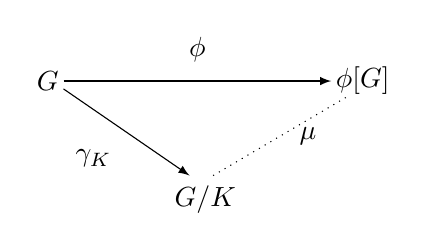
\begin{tikzpicture}
		\draw (0,1.5) node {$G$};
		\draw (2,0) node {$G/K$};
		\draw (4,1.5) node {$\phi[G]$};
		\draw[-latex] (0.2,1.4) -- node(e1)[sloped,label=below:$\gamma_K$]{} (1.8,0.3);
		\draw[-latex] (0.2,1.5) -- node(e2)[label=above:$\phi$]{} (3.6,1.5);
		\draw[dotted] (2.1,0.3) -- node(e2)[label=right:$\mu$]{} (3.8,1.3);
	\end{tikzpicture}
	\caption{First Isomorphism Theorem}
\end{figure}

\subsection{Second Isomorphism Theorem}
\begin{definition}

	Join $H \vee N$ is the smallest subgroup of $G$ containing $HN$ where $HN = \{ hn : h \in H, n \in N\}$.
\end{definition}

\begin{lemma}
	Let $N$ be a normal subgroup of $G$ and let $\gamma : G \to G/N$ be the canonical homomorphism.
	Then the map $\phi$ from the set of normal subgroups of $G$ containing $N$ to the set of normal subgroup of $G/N$ given by $\phi(L) = \gamma[L]$ is one-to-one and onto.
\end{lemma}
\begin{proof}
	Let $G$ be a group and $N$ be a normal subgroup of $G$.
	Given that $\gamma : G \to G/N$ the canonical homomorphism.
	That is, $\gamma(g) = gN$ for every $g \in G$.
	Let $L,M$ be normal subgroups of $G$ containing $N$.
	Since homomorphism preserves normality, $\gamma(L)$ is a normal subgroup of $\gamma[G]$.

	Suppose $\phi(L) = \phi(M)$.
	By definition of $\phi$,
	\begin{equation*}
		\gamma[L] = \phi(L) = \phi(M) = \gamma[M]
	\end{equation*}
	Since $N$ is normal, $\gamma^{-1}(\gamma(g)) = gN$ for every $g \in G$.
	And
	\begin{equation*}
		\gamma^{-1}(\gamma[L]) = \gamma^{-1} \left( \bigcup_{g \in L} \gamma(g) \right) = \bigcup_{g \in L} \gamma^{-1}(\gamma(g)) = \bigcup_{g \in L} gN = L
	\end{equation*}
	for every point $g \in L$, the left coset $gN$ is contained in $L$. ($\because N \subgroup L$)
	Therefore,
	\begin{equation*}
		\gamma^{-1} (\phi(L))  = \gamma^{-1} (\gamma[L]) = L 
	\end{equation*}
	\begin{equation*}
		\gamma^{-1} (\phi(M)) = \gamma^{-1} (\gamma[M]) = M
	\end{equation*}
	Thus, $L = M$.
	Therefore, $\phi$ is injective.

	Let $H$ be a normal subgroup of $G/N$.
	Then $\gamma^{-1}(H)$ is a normal subgroup of $G$.
	We have, $eN \in H$ and $\gamma^{-1}(eN) = eN = N$.
	Thus, $N \subset \gamma^{-1}(H)$.
	Thus, there exists $\gamma^{-1}(H)$, a normal subgroup of $G$ containing $N$ such that $\phi(\gamma^{-1}(H)) = H$.
	Therefore, $\phi$ is surjective.
\end{proof}

\begin{lemma}
	If $N$ is a normal subgroup of $G$, then $H \cap N = HN = NH$.
	Furthermore, if $H$ is also normal in $G$, then $HN$ is normal in $G$.
\end{lemma}
\begin{proof}
	Let $G$ be a group and $N$ be a normal subgroup of $G$.
	Also let $H$ be a subgroup of $G$.\\
	Claim : $HN = \{ hn \in G : h \in H,\ n \in N \}$ is a subgroup of $G$.
	\begin{enumerate}[label=G\arabic*]
		\item Closure : $h_1n_1h_2n_2 = h_1(h_2n_3)n_2 = h_3n_4 \in HN$, where $h_1,h_2 \in H$ and $n_1,n_2,n_4 \in N$. Since $N$ is normal, $n_1h_2 = h_2n_3$ for some $n_3 \in N$.
		\item $HN \subset G$, thus $HN$ satisfies associativity.
		\item Since $H,N \subgroup G$, $e \in H$ and $e \in N$. Thus, $e = ee \in HN$.
		\item Let $h_1n_1 \in HN$. $H \subgroup G$ and $h_1 \in H \implies h_1^{-1} \in H$. Then $n_1^{-1}h_1^{-1} = h_1^{-1}n_2$ for some $n_2 \in N$, since $N$ is normal. Thus, every element in $HN$, $h_1n_1$ has an inverse $h_1^{-1}n_2 \in HN$.
	\end{enumerate}
	Let $H$ be a normal subgroup of $G$.
	Let $g \in G$.
	Then $g(h_1n_1) = (gh_1)n_1 = (h_2g)n_1 = h_2(gn_1) = h_2(n_2g) = (h_2n_2)g$ for some $h_2 \in H$ and $n_2 \in N$ since both $H$ and $N$ are normal subgrops of $G$.
	Thus $gHN = HNg$ for every $g \in G$.
	Therefore, $HN$ is a normal subgroup of $G$.
\end{proof}

\begin{theorem}[second isomorphism]
	Let $H$ be a subgroup of $G$ and let $N$ be a normal subgroup of $G$.
	Then $(HN)/N \isomorphism H/(H\cap N)$.
\end{theorem}
\begin{proof}
	\begin{figure}
		\centering
		\begin{tikzpicture}
			\draw[-latex] (2,2) --node[above]{$\gamma_{|_{HN}}$} (6,2);
			\draw[-latex] (2,2) -- (4,0);
			\draw[dotted] (6,2) --node[left]{$\mu_1$} (4,0);
			\draw[-latex] (10,2) --node[above]{$\gamma_{|_H}$} (6,2);
			\draw[-latex] (10,2) -- (8,0);
			\draw[dotted] (8,0) --node[right]{$\mu_2$} (6,2);
			\draw[dotted] (8,0) --node[above]{$\mu_1 \circ \mu_2^{-1}$} (4,0);
			\draw (1,2) node{$HN$};
			\draw (6,2.5) node{$\gamma[H]$};
			\draw (10.5,2) node{$H$};
			\draw (4,-0.5) node{$HN/N$};
			\draw (8,-0.5) node{$H/H\cap N$};
		\end{tikzpicture}
		\caption{Second Isomorphism Theorem}
	\end{figure}
	Consider the canonical homomorphism $\gamma : G \to G/N$ with kernel $N$.
	Then $\gamma$ restricted to $HN$ is a homomorphism from $HN$ onto $\gamma[H]$.
	\begin{equation}
		\gamma_{|_{HN}} : HN \to \gamma[H] \text{ where } \gamma_{|_{HN}}(hn) = \gamma(hn) = (hn)N = hN = \gamma(h)
	\end{equation}
	Since $\ker(\gamma) = N$ and $N \subset HN$. We have, $\ker(\gamma_{|_{HN}}) = N$. 
	By first isomorphism therorem there exists a unique isomorphism $\mu_1 : HN/N \to \gamma[H]$ where $\mu_1(hnN) = \gamma(h) = hN$.\\

	Similarly, $\gamma$ restricted to $H$ is also a homomorphism onto $\gamma[H]$.
	\begin{equation}
		\gamma_{|_H} : H \to \gamma[H] \text{ where } \gamma_{|_H}(h) = \gamma(h) = hN.
	\end{equation}
	Since $\ker(\gamma) = N$ and $H \cap N \ne \phi$. $\ker(\gamma_{|_H}) = H \cap N$. By first isomorphism theorem, there exists a unique isomorphism $\mu_2 : H/(H\cap N) \to \gamma[H]$% where $\mu_2(h(H \cap N)) = \gamma(h) = hN$.\\

	Then $HN/N \isomorphism H/(H \cap N)$, since the composition of two isomorphisms, $\mu_2^{-1}\circ \mu_1 : HN/N \to H/(H \cap N)$ is an isomorphism% where $\mu_2^{-1}\circ \mu_1 (hnN) = \mu_2^{-1} (\gamma(h)) = \mu_2^{-1} (hN) = h(H \cap N)$.
\end{proof}

\subsection{Third Isomorphism Theorem}
\begin{theorem}[third isomorphism]
	Let $H$ and $K$ be normal subgroup of $G$ with $K \le H$.
	Then $G/H \isomorphism (G/K)/(H/K)$.
\end{theorem}
\begin{proof}
\begin{figure}[h]
	\centering
	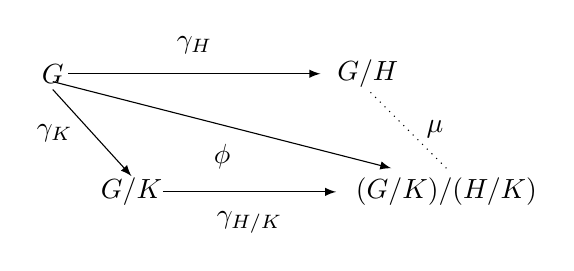
\begin{tikzpicture}
		\draw (0,1.5) node {$G$};
		\draw (1,0) node {$G/K$};
		\draw (5,0) node {$(G/K)/(H/K)$};
		\draw (4,1.5) node {$G/H$};
		\draw[-latex] (0,1.3) -- node(e1)[label=left:$\gamma_K$]{} (1,0.2);
		\draw[-latex] (0.2,1.5) -- node(e2)[label=above:$\gamma_H$]{} (3.4,1.5);
		\draw[-latex] (1.4,0) -- node(e3)[label=below:$\gamma_{H/K}$]{} (3.6,0);
		\draw[-latex] (0,1.4) -- node(e4)[label=below:$\phi$]{} (4.3,0.3);
		\draw[dotted] (5,0.3) -- node(e5)[label=right:$\mu$]{} (4,1.3);
	\end{tikzpicture}
	\caption{Third Isomorphism Theorem}
\end{figure}
	Consider the function $\phi : G \to (G/K)/(H/K)$ defined by $\phi(g) = gK(H/K)$.
	Then, $\phi$ is a homomorphism.
	\begin{align*}
		\phi(ab) & = (ab)K/(H/K) \\
		& = (aK)(bK)\ (H/K),\ \because (ab)K = (aK)(bK) \\
		& = aK(H/K)\ bK(H/K),\ \because (xy)H/K = xH/K\ yH/K\\
		& = \phi(a) \phi(b)
	\end{align*}
	The kernel of $\phi$ is the set $\{ a \in G : \phi(a) = H/K \}$.
	Since the coset $H/K$ was originally the points in $H$, we have $\ker(\phi) = H$.
	By first isomorphism theorem, there exists a unique isomorphism $\mu : G/H \to (G/K)/(H/K)$. Thus, $G/H \isomorphism (G/K)/(H/K)$.
\end{proof}

\section{Finite non-abelian Groups}
\begin{theorem}
	Let $p$ be a prime. Let $G$ be a group of order $p^n$.
	Let $X$ be a finite $G$-set.
	Then $|X| \equiv |X_G| \pmod{p}$.
\end{theorem}
\begin{proof}
	Suppose there are $r$ orbits in $X$.
	Choose an element from each orbit, say $x_1,x_2,\cdots,x_r$.
	We have, 
	\begin{equation}
		|X| = \sum_{i = 1}^r |Gx_i|
	\end{equation}
	Let $X_G = \{ x \in X : gx = x,\ \forall g \in G \}$.
	Then each element in $X_G$ belongs to an orbit of length 1.
	Let $|X_G| = s$. Then,
	\begin{equation}
		|X| = |X_G| + \sum_{i = s+1}^r |Gx_i|
	\end{equation}
	We have, $|Gx| = (G:G_x)$.
	Clearly, both $G$ and $G_x$ are groups of order a multiple of prime $p$.
	Thus, for every $x \in X$, $|Gx|$ is multiple of prime $p$.
	Therefore, $|X| \cong |X_G| \pmod{p}$.
\end{proof}

\begin{definition}
	Let $G$ be a group. Let $p$ be a prime. $G$ is a \textbf{$p$-group} if every element of $G$ has order a power of $p$.
	A subgroup $H$ of $G$ is a \textbf{$p$-subgroup} of $G$ if every element of $H$ has order a power of $p$.
\end{definition}
\begin{theorem}[Cauchy]
	Let $p$ be a prime.
	Let $G$ be a finite group and $p$ divides $|G|$, then $G$ has a subgroup of order $p$.
\end{theorem}
\begin{proof}
	Let $X$ be the set of all $n$-tuples of elements of $G$ such that the product of co-ordinates of each $n$-tuple is the identity element $e$ of $G$.
	\begin{equation}
	X = \{ (g_1,g_2,\cdots,g_p) \in G^p : g_1g_2\cdots g_p = e\}
	\end{equation}
	Let $g_1,g_2,\cdots,g_{p-1}$ be any elements in $G$.
	Then $g_p = (g_1g_2\cdots g_{p-1})^{-1}$ is uniquely determined.
	That is, the $(p-1)$ co-ordinates of an element in $X$ may be chosen in $|G|$ different ways.
	Thus, $|X| = |G|^{p-1}$.
	Since $p$ divides $|G|$, $p$ divides $|X|$.

	We have $g_1(g_2\cdots g_p) = (g_2g_3\cdots g_p)g_1$, since $g_2g_3\cdots g_p = g_1^{-1}$.
	Thus, for every $(g_1,g_2,\cdots,g_p) \in X$, the $\sigma$ permutation of that element is in $X$.
	That is, $\sigma(g_1,g_2,\cdots,g_p) = (g_2,g_3,\cdots,g_p,g_1) \in X$.
	Similarly, $g_2(g_3g_4\cdots g_pg_1) = (g_3g_4\cdots g_pg_1)g_2$.
	And $\sigma^2(g_1,g_2,\cdots,g_p) = g_3,g_4,\cdots,g_p,g_1,g_2)$.
	Clearly, the subgroup generated by $\sigma$, is a subgroup of $S_p$ and $X$ is a $<\!\sigma\!>$-set.
	We have, $|X| \cong |X_{<\sigma>}| \pmod{p}$.
	Thus, $p$ divides $|X_{<\sigma>}|$.

	Clearly, $(e,e,\cdots,e) \in X$ and $(e,e,\cdots,e) \in X_{<\sigma>}$.
	Thus, $X_{<\sigma>}$ has atleast $p$ elements.
	Let $(g_1,g_2,\cdots,g_p) \in X_{<\sigma>}$, then $\sigma$ fixes $(g_1,g_2,\cdots,g_p)$.
	\begin{align*}
		\sigma(g_1,g_2,\cdots,g_p) & = (g_1,g_2,\cdots,g_p)\\
		\implies (g_2,\cdots,g_p,g_1) & = (g_1,g_2,\cdots,g_p)
	\end{align*}
	Thus, $g_1 = g_2 = \cdots = g_p$, say $g \in G$.
	That $(g,g,\cdots,g) \in X$ and $g^p = e$ by the definition of $X$.
	Therefore, $G$ has an element $g$ of order $p$.
\end{proof}
\begin{corollary}
	Let $G$ be a finite group. Then $G$ is a $p$-group if and only if $|G|$ is a power of $p$.
\end{corollary}
\begin{proof}
\end{proof}
\section{Sylow Theorems}

\chapter{ME010102 Linear Algebra}
%Text Books : \cite{hoffman}
%Module 1:
%Vector spaces, subspaces, basis and dimension
%Co-ordinates, summary of row-equivalence, Computations concerning subspaces
%(Chapter 2- 2.1, 2.2, 2.3,2.4 2.5& 2.6 of the text) (20 hours)
%Module 2:
% Linear transformations, the algebra of linear transformations, isomorphism, representation of transformations by matrices, linear functional, double dual, transpose of a linear transformation.
%(Chapter 3 - 3.1, 3.2, 3.3, 3.4, 3.5, 3.6 & 3.7 of the text) (25 hours)
%Module 3:
%Determinants: Commutative Rings, Determinant functions, Permutation and uniqueness of determinants, Additional properties of determinants.
%(Chapter 5 - 5.1, 5.2, 5.3 & 5.4 of the text) (20 hours)
%Module 4:
%Introduction to elementary canonical forms, characteristic values, annihilatory Polynomials, invariant subspaces, Direct sum Decompositions
%(Chapter 6 - 6.1, 6.2, 6.3, 6.4,6.6of the text) (25 hours)

% \cite{hoffman} 2, 3, 5, 6
%Missing - 1, 4, 7, 8, 9, 10

%Module 1 - \cite{hoffman} 2
\section{Vector Spces}
%Module 2 - \cite{hoffman} 3
\section{Linear Transformations}
%Module 3 - \cite{hoffman} 5
\section{Determinants}
%Module 4 - \cite{hoffman} 6
\section{Elementary Canonical Forms}

\chapter{ME010103 Basic Topology}
%Text Books : \cite{joshi}
%Module I :
%Topological Spaces: Definition of a topological space – Examples of topological spaces-Bases and subbases – subspaces.
%(Chapter 4: Sections 1, 2, 3, and 4 of the text) (25 hours)
%Module II :
%Basic concepts: Closed sets and Closures – Neighbourhoods, Interior and
%Accumulation points – Continuity and Related Concepts – Making functions continuous , Quotient spaces
%( Chapter 5: Section 1;1. To 1.7 , Section 2; 2.1 to 2.10 and 2.13, Section3; 3.1 to 3.11, Theorem 3.2 condition 4 (25 hours)
%Module III :
%Spaces with special properties :- Smallness conditions on a space, Connectedness
%( Chapter 6 : Section 1; 1.1 to 1.16, Section 2; 2.1 to 2.15) (20 hours)
%Module IV :
%Spaces with special properties :- Local connectedness and Paths
%Separation axioms:- Hierarchy of separation axioms
%( Chapter 6 : Sections 3.1 to 3.8, Chapter 7 : Sections 1.1 to 1.17(20 hours)

%\chapter{Logical Warm-up*}
%\section{Statements and Their Truth values}
%\section{Negation, Conjunction, Disjunction and Truth Tables}
%\section{Deductions and Logical Precision}

%\chapter{Preliminaries}
%\section{Sets and Functions}
%\section{Sets with Additional Structures}
%\section{Preliminaries from Analysis}

%\chapter{Motivation for Topology}
%\section{What is Topology ?}
%\section{Geometry and Topology}
%\section{From Geometry to Metric Spaces}

%Introduction to topology game
%1. Open set characterisation
%Make four subsets of alphabets
%Letters of your name, and three of your friends names
%Intersection of any two sets - closed under finite intersections
%Union of any two sets - closed under arbitrary union
%2. Closed set characterisation
%Letters not in your name, and three of your friends names
%Union of any two sets - closed under finite unions
%Intersection of any two sets - closed under arbitrary intersections
%3. Neighbourhood Characterisation
%4. Interior Characterisation

%Need to find activities for the following :
%Continuous Function \& Quotient Space
%Compact, Lindeloff - Smallness of a Space
%Connected, Locally Connected, Path Connected
%Separation Axioms

%Need to give reading assignments:
%relevent skipped portions - what we might have missed !?
%other reference books - how they are presenting the same idea ?
%other books - get meaning out of it !

\part{ME010103 Basic Topology}
\chapter{Topological Spaces}
\section{Definition of a Topological Space}
\section{Examples of Topological Spaces}
\section{Bases and Sub-bases}
\section{Subspaces}

\chapter{Basic Concepts}
\section{Closed Sets and Closure}
\section{Neighbourhoods, Interior and Accumulation Points}
\section{Continuity and Related Concepts}
\section{Making Functions Continuous, Quotient Spaces}

\chapter{Spaces with Special Properties}
\section{Smallness Conditions on a Space}
\section{Connectedness}
\section{Local Connectedness and Paths}

\chapter{Separation Axioms}
\section{Hierarchy of Separation Axioms}

\chapter{ME010103 Real Analysis}
%Text Books: \cite{apostol}, \cite{rudin}
%Module 1: Functions of bounded variation and rectifiable curves
%Introduction, properties of monotonic functions, functions of bounded variation, total variation, additive property of total variation, total variation on $(a,x)$ as a functions of $x$, functions of bounded variation expressed as the difference of increasing functions, continuous functions of bounded variation, curves and paths, rectifiable path and arc length, additive and continuity properties of arc length, equivalence of paths, change of parameter.
%(Chapter 6, Section: 6.1 - 6.12. of \cite{apostol}) (20 hours.)
%Module 2: The Riemann-Stieltjes Integral
%Definition and existence of the integral, properties of the integral, integration and differentiation, integration of vector valued functions.
%(Chapter 6 - Section 6.1 to 6.25 of \cite{rudin}) (20 hours.)
%Module 3: Sequence and Series of Functions
%Discussion of main problem, Uniform convergence, Uniform convergence and Continuity, Uniform convergence and Integration, Uniform convergence and Differentiation.
%(Chapter 7 Section. 7.1 to 7.18 of \cite{rudin}) (25 hours.)
%Module 4: Weierstrass Approximation \& Some Special Functions
%Equicontinuous families of functions, the Stone - Weierstrass theorem, Power series, the exponential and logarithmic functions, the trigonometric functions, the algebraic completeness of complex field.
%(Chapter 7 – Sections 7.19 to 7.27, Chapter 8 - Section 8.1 to 8.8 of \cite{rudin}) (25 hours.)

%Module 1 - \cite{apostol} 6
%Module 2 - \cite{rudin} 6
%Module 3 - \cite{rudin} 7a
%Module 4 - \cite{rudin} 7b

%The commands to Riemann upper/lower integrals are defined by Leo Liu in tex-stack-exchange.
%Leo Liu - https://tex.stackexchange.com/a/44245 
\def\upint{\mathchoice%
    {\mkern13mu\overline{\vphantom{\intop}\mkern7mu}\mkern-20mu}%
    {\mkern7mu\overline{\vphantom{\intop}\mkern7mu}\mkern-14mu}%
    {\mkern7mu\overline{\vphantom{\intop}\mkern7mu}\mkern-14mu}%
    {\mkern7mu\overline{\vphantom{\intop}\mkern7mu}\mkern-14mu}%
  \int}
\def\lowint{\mkern3mu\underline{\vphantom{\intop}\mkern7mu}\mkern-10mu\int}

%Module 1
%\chapter{Functions of Bounded Variation \& Rectifiable Curves}
{\Large Module 1 : Bounded Variation \& Rectifiable Curves}
\section{Functions of Bounded Variation \& Rectifiable Curves}
%\subsection{Introduction}
\setcounter{subsection}{1}
\subsection{Properties of Monotone Functions}
\begin{theorem}
	Let $f$ be an increasing function defined on closed interval $[a,b]$.
	And let $x_0=a < x_1 < x_2 < \dots <x_{n-1} < x_n = b$.
	Then,
	\[ \sum_{k = 1}^{n-1} [f(x_k+)-f(x_k-)] \le f(b) - f(a) \]
\end{theorem}
\begin{proof}
	Let $f$ be an increasing function on $[a,b]$.
	Let $\{x_0=a,\ x_1, \dots,\ x_n=b\}$ be a partition of $[a,b]$.
	Let $y_k \in (x_{k-1},x_k),\ \forall k$.
	Then, $f(y_k) \le f(x_k+)$ and $f(x_k-) \le f(y_{k-1})$.
	Therefore,
	\[ \sum_{k=1}^{n-1} [f(x_k+) - f(x_k-)] \le \sum_{k=1}^{n-1} [f(y_k) - f(y_{k-1})] \le f(b) - f(a) \]
\end{proof}
\begin{commentary}
	In other words, for monotonic functions the sum of jumps is bounded.
\end{commentary}

\begin{theorem}
	Let $f$ be a monotonic function defined on closed interval $[a,b]$.
	Then the set of discontinuities of $f$ is countable.
\end{theorem}
\begin{proof}
	Without loss of generality, let $f$ be an increasing function on $[a,b]$.
	Let $S_m$ be the set of all points on $[a,b]$ at which the jump exceeds $\frac{1}{m}$.\\

	We know that, the sum of jumps of an increasing function is bounded above by $f(b)-f(a)$.	
	Thus, cardinality of $S_m$ given by,
	\[ |S_m| < m[f(b)-f(a)] \]
	is finite for any positive integer $m$.\\

	If $f$ is discontinuous at a pont $x \in [a,b]$, then there exists some integer $m'$ such that $0 < \frac{1}{m'} < x $ and $x \in S_{m'}$.
	\[ \text{Number of discontinuities } = \left| \bigcup_{m=1}^\infty S_m \right| \le \sum_{m=1}^\infty |S_m| \text{ is countable.}\]
	since countable sum of finite values is countable.
	Therefore, the number of discontinuities of $f$ is countable.
\end{proof}

\subsection{Function of Bounded Variation}
\begin{definition}[partition]
	Let $[a,b]$ be a compact interval.
	Let $x_0 = a$, $x_0 < x_1 < x_2 < \dots < x_n$ and $x_n = b$.
	Then $P = \{ x_0,x_1,\dots,x_n \}$ is a \textbf{partition} of $[a,b]$.
	And $(x_{k-1},x_k)$ is the \textbf{$k$th subinterval} of the partition.
\end{definition}

\begin{definition}[bounded variation]
	Let $f$ be a function defined on closed interval $[a,b]$.
	If there exists a positive real-number $M$ such that
	\[ \sum_{k=1}^n |\Delta f_k| = \sum_{k=1}^n |f(x_k) - f(x_{k-1})| \le M \]
	for any partition $P$ on $[a,b]$.
	Then $f$ is a function of \textbf{bounded variation}, where $(x_{k-1},x_k)$ is the $k$th subinterval of the partition.\\

\begin{commentary}
	In other words, a function is of bounded variation on $[a,b]$ if the sum of variations is bounded for any (finite) partition of $[a,b]$.
\end{commentary}
\end{definition}

\begin{theorem}
	Let $f$ be a monotonic function on $[a,b]$.
	Then $f$ is of bounded variation on $[a,b]$.
\end{theorem}
\begin{proof}
	Without loss of generality, let $f$ be an increasing function.
	Then for any partition $P = \{x_0,x_1,\dots,x_n\}$ of $[a,b]$, we have
	\[ \sum_{k=1}^n \left[ f(x_k)-f(x_{k-1}) \right] \le f(b)-f(a) = M \]
	Therefore, $f$ is of bounded variation on $[a,b]$.
\end{proof}

\begin{theorem}
	Let $f$ be a continuous function on $[a,b]$ and its derivative $f'$ exists and $f'$ is bounded in $(a,b)$.
	Then $f$ is of bounded variation.	
\end{theorem}
\begin{proof}
	Let $f$ be a continuous function with derivative $f'$ on $(a,b)$.
	Since $f$ is continuous and $f'$ exists, from intermediate value theorem we have
	\[ \Delta f_k = f(x_k) - f(x_{k-1}) = f'(t_k) [x_k-x_{k-1}] \text{ where } t_k \in (x_{k-1},x_k) \]
	Since $f'$ is bounded, $f'(t_k) \le M'$ for any $t_k \in (a,b)$.
	Thus,
	\[ \sum_{k=1}^n |\Delta f_k| = \sum_{k=1}^n |f'(t_k)| (x_k-x_{k-1}) \le M'\sum_{k=1}^n x_k-x_{k-1} = M'(b-a) = M \]
	Therefore, $f$ is of bounded variation.
\end{proof}

\begin{theorem}
	Let $f$ be a function on $[a,b]$.
	If $f$ is of bounded variation, then $f$ is bounded.
\end{theorem}
\begin{proof}
	Let $x \in (a,b)$.
	Consider the partition $P = \{ a,x,b \}$.
	Since $f$ is of bounded variation, there exists a positive real-number $M$ such that
	\[ \sum_{k=1}^2 |\Delta f_k| = |f(x)-f(a)| + |f(b)-f(x)| \le M \]
	Clearly, $|f(x)-f(a)| \le M$, since $|f(b)-f(x)| > 0$.
	We have,
	\[ |f(x)| = |f(x)-f(a)+f(a)| \le |f(x)-f(a)|+|f(a)| \le M+|f(a)| \]
	Suppose $x = a$, then $|f(x)| = |f(a)|$.\\
	Suppose $x = b$, then $|f(x)| = |f(b)| = M' + |f(a)|$ where $M' = |f(b)|-|f(a)|$.\\

	Therefore, the function $f$ is bounded on $[a,b]$.
\end{proof}

\subsection{Total Variation}
\begin{definition}[total variation]
	Let $f$ be a function of bounded variation on $[a,b]$.
	Let $\Sigma (P)$ be the sum of variations with respect to the partition $P$ of $[a,b]$.
	Then the \textbf{total variation} of the function $f$ on $[a,b]$ is given by,
	\[ V_f(a,b) = V_f = \sup \{ \Sigma (P) : P \in \mathscr{P}[a,b] \} \]
\end{definition}
\textbf{Note 1} : $V_f$ is finite, since $f$ is of boundned variation on $[a,b]$.\\

\textbf{Note 2} : $V_f \ge 0$, since $|\Delta f_k| \ge 0$ for any subinterval of $[a,b]$.\\


\textbf{Note 3} : $V_f = 0$ if only if $f$ is a constant function on $[a,b]$. (Why ?)

\begin{theorem}
	Let $f,g$ be functions of bounded variation on $[a,b]$.
	Then their sum $f+g$, difference $f-g$, and product $fg$ are of bounded variation.
	Also, 
	\[ V_{f \pm g} \le V_f + V_g \quad \text{ and } \quad V_{fg} \le AV_f + BV_g \]
	where $\displaystyle A = \sup \left\{ |g(x)| : x \in [a,b] \right\}$ and $\displaystyle B = \sup \left\{ |f(x)| : x \in [a,b] \right\}$.
\end{theorem}
\begin{proof}
	Let $f,g$ be functions of bounded variation on $[a,b]$.
	Then $f,g$ are bounded and $\sup |f(x)|$ and $\sup |g(x)|$ exists.\\

	\textbf{Step 1 : $V_{f \pm g} \le V_f + V_g$}\\
	We have,
	\[ |(f+g)(x_k) - (f+g)(x_{k-1})| \le | f(x_k) - f(x_{k-1})| + |g(x_k) - g(x_{k-1})| \]
	Then
	\begin{align*}
	V_{f+g}  
		& = \sup_{P \in \mathscr{P}} \sum_{k=1}^n |(f+g)(x_k) - (f+g)(x_{k-1})| \\
		& \le \sup_{P \in \mathscr{P}} \sum_{k=1}^n |f(x_k) - f(x_{k-1})| + \sup_{P \in \mathscr{P}} \sum_{k=1}^n |g(x_k)-g(x_{k-1})| \\
		& = V_f + V_g 
\end{align*}
	Similarly, we have $V_{f-g} \le V_f + V_g$ since
	\[ |(f-g)(x_k) - (f-g)(x_{k-1})| \le |f(x_k)-f(x_{k-1})| + |g(x_k)-g(x_{k-1})| \]

	\textbf{Step 2 : $V_{fg} \le AV_f + BV_g$}\\
	We have,
	\begin{align*}
	|fg(x_k)-fg(x_{k-1})| 
		& = |f(x_k)g(x_k) - f(x_{k-1}g(x_{k-1})| \\
		& = |f(x_k)g(x_k) - f(x_{k-1})g(x_k) + f(x_{k-1}g(x_k) - f(x_{k-1}g(x_{k-1}) | \\
		& \le |g(x_k)|\ |f(x_k)-f(x_{k-1})| + |f(x_{k-1}|\ |g(x_k) - g(x_{k-1})| \\
		& \le A |f(x_k)-f(x_{k-1})| + B |g(x_k)-g(x_{k-1})|
	\end{align*}
	where $A = \sup \{ |g(x)| : x \in [a,b] \}$ and $B = \sup \{ |f(x)| : x \in [a,b] \}$.\\

	Therefore,
	\begin{align*}
	V_{fg} 
		& \le A \sup_{P \in \mathscr{P}} \left\{ \sum_{k=1}^n |f(x_k)-f(x_{k-1}| \right\} + B \sup_{P \in \mathscr{P}} \left\{ \sum_{k=1}^n |g(x_k)-g(x_{k-1})| \right\} \\
		& = AV_f + BV_g 
	\end{align*}
\end{proof}

\begin{definition}[bounded away from zero]
	A function $f$ is bounded away from zero on $[a,b]$ if there exists a real-number $m$ such that $0 < m \le f(x)$, $\forall x \in [a,b]$.
\end{definition}

\begin{commentary}
	Let $f$ be a function of bounded variation.
	Then $\frac{1}{f}$ is of bounded variation if and only if $f$ is bounded away from zero.(Why ?)
\end{commentary}

\begin{theorem}
	Let $f$ be a function of bounded variation on $[a,b]$ and $f$ is bounded away from zero.
	Then, $g = \frac{1}{f}$ is a function of bounded variation on $[a,b]$ and $V_g \le \frac{V_f}{m^2}$ whenever $0 < m \le |f(x)|$.
\end{theorem}
\begin{proof}
	Suppose $f$ is of bounded variation on $[a,b]$ and $f$ is bounded away from zero.
	That is, there exists positive real-number $m$ such that $0 < m \le |f(x)|$, $\forall x \in [a,b]$.
	Then, $\frac{1}{|f(x)|} \le \frac{1}{m}$, $\forall x \in [a,b]$.\\

	Define $g = \frac{1}{f}$.
	Then, we have
	\[ |\Delta g_k| = \left| \frac{1}{f(x_k)} - \frac{1}{f(x_{k-1})} \right| = \frac{|f(x_k)-f(x_{k-1})|}{|f(x_k)|\ |f(x_{k-1}|} \le \frac{|f(x_k)-f(x_{k-1})|}{m^2} \]
	The total variation of $g$ on $[a,b]$ is given by,
	\begin{align*}
	V_g 
		& = \sup_{P \in \mathscr{P}} \left\{ \sum_{k=1}^n |g(x_k)-g(x_{k-1})| \right\} \\
		& \le \frac{1}{m^2} \sup_{P \in \mathscr{P}} \left\{ \sum_{k=1}^n |f(x_k)-f(x_{k-1})| \right\} \\
		& \le \frac{V_f}{m^2} \text{ where } 0 < m \le |f(x)|,\ \forall x \in [a,b]
	\end{align*}
\end{proof}
\begin{commentary}
	In other words, if $h,f$ are functions of bounded variation of $[a,b]$.
	And $f$ is bounded away from zero, then $g = \frac{1}{f}$ and $\frac{h}{f} = hg$ is a function of bounded variation and $V_{\frac{h}{f}} = V_{hg} \le AV_h + BV_f$.\\

	Now, we have analyzed sum, difference, product and quotient of functions of bounded variation.
	And we are not surprised about preservation of bounded variation under function composition. (Why ?)
\end{commentary}
\subsection{Additive Property of Total Variation}
\begin{theorem}[additive property]
	Let $f$ be a function of bounded variation on $[a,b]$.
	Let $c \in (a,b)$.
	Then $f$ is of bounded variation on both $[a,c]$ and $[c,b]$.
	And, $V_f(a,b) = V_f(a,c)+V_f(c,b)$.
\end{theorem}
\begin{proof}
	Let $f$ be a function of bounded variation on $[a,b]$.
	Let $P_1,P_2$ be partitions of $[a,c]$ and $[c,b]$ respectively.
	Then $P_0 = P_1 \cup P_2$ is a partition of $[a,b]$.
	Thus,
	\[ \sum (P_1) + \sum (P_2) = \sum (P_0) \le V_f(a,b) \]
	Taking supremums on the left side, we get
	\[ V_f(a,c) + V_f(c,b) \le V_f(a,b) \]	
	Clearly, $V_f(a,c) \le V_f(a,b)$ and $V_f(c,b) \le V_f(a,b)$.
	Therefore, function $f$ is of bounded variation on both $[a,c]$ and $[c,b]$.\\

	Let $P$ be a paritition of $[a,b]$.
	Then $P_0 = P\cup\{c\}$ is refinement of $P$.
	Now, we have two partitions $P_1, P_2$ of $[a,c]$ and $[c,b]$ such that $P_0 = P_1 \cup P_2$.
	Thus,
	\[ \sum (P) \le \sum (P_0) = \sum (P_1) + \sum (P_2) \le V_f(a,c) + V_f(c,b) \]
	Taking supremum on the left side, we get
	\[ V_f(a,b) \le V_f(a,c) + V_f(c,b) \]
	Therefore,
	\[ V_f(a,b) = V_f(a,c) + V_f(c,b),\quad \forall c \in (a,b) \]
\end{proof}

\subsection{Total Variation on $[a,x]$ as a function of $x$}
\begin{commentary}
	By additive property, we have existence of $V_f(a,x)$ for every $x \in (a,b]$.
	Assigning $V(x) = V_f(a,x)$, we have a well-defined function on $(a,b]$.
\end{commentary}

\begin{theorem}
	Let $f$ be a function of bounded variation on $[a,b]$.
	Define $V : [a,b] \to \mathbb{R}$ given by,
	\[ V(x) = \begin{cases} V_f(a,x) & x \in (a,b] \\ 0 & x = a \end{cases} \]
	Then,
	\begin{enumerate}
		\item $V$ is an increasing function on $[a,b]$.
		\item $V-f$ is an increasing function of $[a,b]$.
	\end{enumerate}
\end{theorem}
\begin{proof}
	Suppose $x = a$.
	Then $V(x) = 0$ and $V(y) = V_f(a,y) \ge 0 = V(x)$.\\
	Suppose $x \ne a$.
	Then, $a < x < y \le b$.
	By additive property of total variation, we have $V(y) = V_f(a,y) = V_f(a,x)+V_f(x,y) = V(x) + V_f(x,y)$.
	Since $V_f(x,y) \ge 0$, we have $V(x) \le V(y)$.
	Therefore, $V$ is an increasing function on $[a,b]$.\\

	Define $D : [a,b] \to \mathbb{R}$ given by $D(x)  = (V-f)(x) = V(x) - f(x)$.
	Suppose $a \le x < y \le b$.
	Then, $D(y)-D(x) = V(y)-f(y)-V(x)+f(x) = [V(y)-V(x)] - [f(y)-f(x)]$.
	We have, $V(y) = V_f(a,y) = V_f(a,x)+V_f(x,y)$.
	Thus, $V(y)-V(x) = V_f(x,y)$.
	Also we have, $f$ is of bounded variation on $[x,y]$.
	Consider the trivial partition $P = \{ x,y\}$ of $[x,y]$.
	Then, we have $f(y) - f(x) = \sum (P) \le V_f(x,y)$.
	Thus, $D(y)-D(x) = V_f(x,y) - [f(y)-f(x)] \ge 0$.
	Therefore, $D = V-f$ is an increasing function on $[a,b]$.
\end{proof}

\subsection{Function of bounded variation expressed as the difference of increasing functions}
\begin{theorem}
	Let $f$ be a function on $[a,b]$.
	Function $f$ is of bounded variation on $[a,b]$ if and only if $f$ can be expressed as difference of two increasing functions.
\end{theorem}
\begin{proof}
	Let $f$ be a function of bounded variation, then $f = V-D$ where total variation $V$ and $D = V-f$ are both increasing.\\

	Let $f$ be function on $[a,b]$.
	Let $f = V-D$ where $V,D$ are increasing functions. 
	Then $V,D$ are of bounded variation, since monotonic functions on $[a,b]$ are of bounded variation.
	Also, we have $V-D$ is of bounded variation, since for any two functions of bounded variation their difference is also of bounded variation.
\end{proof}

\subsection{Continuous functions of bounded variation}
\begin{theorem}
	Let $f$ be a function of bounded variation on $[a,b]$. %Why it has to be of bounded variation ? For the existence of $V$ ?
	Let $V$ be the total variation function of $f$ defined on $[a,b]$.
	$f$ is continuous at a point if and only if $V$ is continuous at that point.
\end{theorem}
\begin{proof}
	Let $f$ be a function of bounded variation on $[a,b]$.
	Let $V$ be the total variation of $f$.
	Let $x,y \in [a,b]$, such that $x<y$.
	We have $V$ is an increasing function on $[a,b]$.
	And $f$ is difference of two increasing functions on $[a,b]$.
	Thus, $f(x+),\ f(x-),\ V(x+),\ V(x-)$ exists for any $x \in (a,b)$.
	It remains to prove that $V,f$ are continuous at $x \in (a,b)$.\\

	\textbf{Part 1 : $V$ continuous $\implies$ $f$ continuous}\\
	Suppose $x \ne a$, then $a<x<y\le b$.
	Let $P$ be any partition on $[a,x]$.
	Then there exists a partition $P'$ on $[a,y]$ such that $P \subset P'$.
	Consider, $P' = P\cup\{y\}$.
	Then, $V(y) > V(x)$ and $V(y)-V(x) \ge |f(y)-f(x)|$.
	Thus,
	\[ 0 \le |f(y)-f(x)| \le V(y)-V(x) \]
	The inequality is true for any $y>x$.
	Therefore,
	\[ 0 \le |f(x+)-f(x)| \le V(x+)-V(x) \text{ as } y \to x+ \]
	Similarly, let $a<z<x$.
	Then,
	\[ 0 \le |f(x)-f(x-)| \le V(x)-V(x-) \text{ as } z \to x- \]
	Clearly, if $V$ is continuous at $x$ then $f$ is continuous $x$.\\

	\textbf{Part 2 : $f$ continuous $\implies$ $V$ continuous}\\
	Suppose $f$ is continuous at $c \in (a,b)$.
	Let $\varepsilon > 0$.
	We have,
	\[ V_f(c,b) = \sup_{P \in \mathscr{P}} \sum (P) \]
	Thus, there exists a partition $P_1 \in \mathscr{P}[c,b]$ such that $V_f(c,b) - \frac{\varepsilon}{2} < \sum (P_1)$.
	Since $f$ is continuous at $c$, there exists $x_1 \in (c,b)$ such that $|f(x_1)-f(c)| < \frac{\varepsilon}{2}$.
	Then,
	\[ V_f(c,b) - \frac{\varepsilon}{2} < \frac{\varepsilon}{2} + V_f(x_1,b) \]
	We have,
	\begin{align*}
	V(x_1)-V(c) 
		& = V_f(a,x_1) - V_f(a,c) = V_f(c,x_1) \\
		& = V_f(c,b) - V_f(x_1,b) < \varepsilon
	\end{align*}
	Clearly, $V(c+h) \to V(c)$ as $h \to 0$.
	That is, $V(c+) = V(c),\ \forall c \in [a,b)$.
	Similarly we have,
	\[ V_f(a,c) = \sup_{P \in \mathscr{P}} \sum (P) \]
	And there exists $P_2 \in \mathscr{P}[a,c]$ such that
	\[ V_f(a,c) - \frac{\varepsilon}{2} < \sum (P_2) \]
	And there exists $x_2 \in (a,c)$ such that $|f(c)-f(x_2)| < \frac{\varepsilon}{2}$, since $f$ is continuous at $c$.
	Therefore,
	\[ V(c)-V(x_2) = V_f(a,c) - V_f(a,x_2) = V(x_2,c) < \varepsilon \]
	Thus, $V(c-) = V(c),\ \forall c \in (a,b]$.
	Therefore, $V$ is continuous at $c$.
\end{proof}
\begin{theorem}
	Let $f$ be a continuous function on $[a,b]$.
	Function $f$ is of bounded variation on $[a,b]$ if and only if $f$ can be expressed as difference of two increasing continuous functions.
\end{theorem}
\begin{proof}
	Let $f$ be a continuous function on $[a,b]$.
	Then total variation $V$ is a continuous increasing function on $[a,b]$.
	Clearly, $D = V-f$ is also a continuous, increasing function on $[a,b]$.
	Therefore, $f = V - D$ where $V,D$ are continuous, increasing functions.\\

	Let $V,D$ be continuous, increasing functions on $[a,b]$.
	Then $f = V-D$ is also a continuous function on $[a,b]$.
	We have, $V,D$ are increasing functions, therefore both $V,D$ are of bounded variation and their difference $f$ is also of bounded variation.
\end{proof}

\begin{commentary}
	Suppose $f$ is of bounded variation on $[a,b]$.
	Let $id : [a,b] \to [a,b]$ where $id(x) = x$.
	Then $V+id$ is a strictly increasing function and $D = V+id-f$ is also strictly increasing.
	Thus, any function of bounded variation on $[a,b]$ can be characterised as difference of two strictly increasing continuous functions on $[a,b]$.
\end{commentary}
\subsection{Curves and Paths}
\begin{definition}[path]
	Let $f : [a,b] \to \mathbb{R}^n$ be a continuous, vector-valued function.
	Then $f$ is a path in $\mathbb{R}^n$.
	And $f$ is a motion if $[a,b]$ is a time interval.
\end{definition}
\subsection{Rectifiable paths and Arc length}
\begin{definition}[rectifiable path]
	Let $f : [a,b] \to \mathbb{R}^n$ be a path in $\mathbb{R}^n$.
	Let $P = \{ t_0,t_1,\dots,t_m \}$ be a partition of $[a,b]$.
	\[ \Lambda_f (P) = \sum_{k=1}^m \| f(t_k) - f(t_{k-1}) \| = \sum_{k=1}^m \| \Delta f_k \| \]
	If $\Lambda_f (P)$ is bounded for any partition $P \in \mathscr{P}[a,b]$, then path $f$ is \textbf{rectifiable}.
	If $\Lambda_f (P)$ is unbounded, then $f$ is \textbf{nonrectifiable}.\\
\end{definition}
\begin{definition}[arc length]
	Let $f : [a,b] \to \mathbb{R}^n$ be a rectifiable path.
	Then \textbf{arc length} of path $f$ is given by,
	\[ \Lambda_f(a,b) = \sup_{P \in \mathscr{P}} \Lambda_f (P) \]
\end{definition}

\begin{theorem}
	A path $f : [a,b] \to \mathbb{R}^n$ is rectifiable if and only if each component $f_k$ of $f$ is of bounded variation on $[a,b]$.
	Let $V_k(a,b)$ be the total variation of $f_k$ on $[a,b]$.
	Then,
	\[ V_k(a,b) \le \Lambda_f(a,b) \le V_1(a,b) + V_2(a,b) + \dots + V_n(a,b) \]
\end{theorem}
\begin{proof}
	Let $x_j \in \mathbb{R}^n$ for $j = 1,2,\dots,m$.
	Then,
	\[ |x_r| \le \sqrt{\sum_{j=1}^n |x_j|^2} \le \sum_{j=1}^n |x_j| \text{ since } \sum_{j=1}^n x_j^2 \le \left(\sum_{j=1}^n x_j\right)^2 \]
	Let $f : [a,b] \to \mathbb{R}^n$ be a path in $\mathbb{R}^n$.
	Then $f = (f_1,f_2,\dots,f_n)$ where $f_k$'s are components of the path $f$.
	Let $P = \{ t_0,t_1,\dots,t_m \}$ be a partition of $[a,b]$.
	Now $f_r(t_j)-f_r(t_{j-1}) \in \mathbb{R}^n$ for each subinterval of $[a,b]$ and each component of $f$.
	Thus for each subinterval $(t_j,t_{j-1})$ we have,
	\[ |f_r(t_j)-f_r(t_{j-1})| \le \| f(t_j)-f(t_{j-1}) \| \le \sum_{j=1}^n |f_k(t_j)-f_k(t_{j-1})| \] 
	Adding inequalities for every subinterval of the partition, we get
	\[ \sum_{k=1}^m |f_k(t_j)-f_k(t_{j-1})| \le \sum_{k=1}^m \| f(t_j)-f(t_{j-1}) \| \le \sum_{k=1}^m \sum_{j=1}^n |f_k(t_j)-f_k(t_{j-1})| \] 
	Rearranging summation, we get
	\[ \sum (P) \le \Lambda_f (P) \le \sum_{j=1}^n \left( \sum (P)_{f_j} \right) \] 
	Suppose $f$ is a rectifiable path.
	Then $f$ has finite arc length $\Lambda_f (a,b)$.
	Let $f_k$ be a component function of $f$.
	Let $P$ be a partition of $[a,b]$.
	Then,
	\[ \sum (P) \le \Lambda_f(P) \le \Lambda_f (a,b) \]
	Thus, $\sum (P)$ is bounded for any partition $P$.
	Therefore, total variation $V_k(a,b)$ exists for each component function $f_k$.
	And $V_k(a,b) \le \Lambda_f(a,b)$.\\

	Suppose $f_k$'s are of bounded variation.
	Then \[ \Lambda_f(P) \le \sum_{j=1}^n \sum (P) \le \sum_{j=1}^n V_j(a,b) \] is bounded for any partition $P$.
	Thus, $f$ is rectifiable.
	And, arc length $\displaystyle \Lambda_f(a,b) \le \sum_{k=1}^n V_k (a,b)$.
	Combining the inequalities, we get
	\[ V_k(a,b) \le \Lambda_f(a,b) \le \sum_{j=1}^n V_j (a,b) \]
\end{proof}
\subsection{Additive and Continuity Properties of Arc length}
\begin{theorem}[additive]
	Let $f : [a,b] \to \mathbb{R}^n$ be a rectifiable path.	
	Let $c \in (a,b)$.
	Then,
	\[ \Lambda_f(a,b) = \Lambda_f(a,c) + \Lambda_f(c,b) \]
\end{theorem}
\begin{proof}
	Let $P$ be a partition of $[a,b]$.
	Then $P' = P \cup \{c\}$ is a refinement of $P$ such that $P' = P_1 \cup P_2$ where $P_1,P_2$ are partition of $[a,c]$ and $[c,b]$ respectively.
	We have,
	\[ \Lambda_f(P) \le \Lambda_f(P') = \Lambda_f(P_1) + \Lambda_f(P_2) \]
	This inequality if true for any partition of $[a,b]$.
	Thus,
	\[ \Lambda_f(a,b) \le \Lambda_f(a,c) + \Lambda_f(c,b) \]
	Let $P_1,P_2$ be partition of $[a,c]$ and $[c,b]$ respectively.
	Then,
	\[ \Lambda_f(P_1) + \Lambda_f(P_2) \le \Lambda_f(P) \le \Lambda_f(a,b) \]
	This inequality if true for any paritions on $[a,c]$ and $[c,b]$.
	Thus,
	\[ \Lambda_f(a,c) + \Lambda_f(c,b) \le \Lambda_f(a,b) \]
\end{proof}
\begin{theorem}[continuity]
	Let $f : [a,b] \to \mathbb{R}^n$ be  rectifiable path.
	Let function $s : [a,b] \to \mathbb{R}$ defined by
	\[ s(x) = \begin{cases} 0 & x = a \\ \Lambda_f(a,x) & x \in (a,b] \end{cases} \]
	Then,
	\begin{enumerate}
		\item function $s$ is continuous and increasing on $[a,b]$.
		\item if there is no subinterval of $[a,b]$ in which $f$ is constant, then $s$ is strictly increasing.
	\end{enumerate}
\end{theorem}
\begin{proof}
	Let $a \le x < y \le b$.
	Then, $s(y)-s(x) = \Lambda_f(x,y) = \Lambda(a,y) - \Lambda(a,x) \ge 0$.
	Therefore, $s$ in increasing.\\
	
	Suppose $f$ is not constant in any subinterval $[x,y]$ of $[a,b]$.
	Suppose $s$ is not strictly increasing.
	Then, there exists $x,y \in (a,b)$ such that $x < y$ and $s(y)-s(x) = 0$.
	Thus,
	\[ \Lambda_f(a,y) - \Lambda(a,x) = \Lambda_f(x,y) = 0 \]
	Thus, $V_k(x,y) = 0,\ \forall k$ which is a contradition since $f$ is not constant in $[x,y]$.
	Therefore, $s$ is strictly increasing.
\end{proof}
\subsection{Equivalence of path, Change of parameter}
\begin{definition}[change of parameter]
	Let $f:[a,b] \to \mathbb{R}^n$ be a path.
	Let $g : [c,d] \to \mathbb{R}^n$ be another path.
	Then $f,g$ are \textbf{equivalent} if there exists a continuous, real-valued function, $u : [c,d] \to [a,b]$ such that $g = f \circ u$.
	That is, $g(t) = f(u(t)),\ \forall t \in [c,d]$.
	In other words, $f,g$ are different parametric representations of a common graph.\\

	Function $u$ defines a change of parameter.
	If $u$ is strictly increasing, then $f,g$ are in the same direction.
	And $u$ is an orientation preserving change of parameter.
	If $u$ is strictly decreasing, then $f,g$ are in opposite directions.
	And $u$ is an orientation reversing change of parameter.
\end{definition}

\begin{theorem}[change of parameter]
	Let $f:[a,b] \to \mathbb{R}^n$ and $g : [a,b] \to \mathbb{R}^n$ be two paths.
	Let $f,g$ be both injective functions.
	Then $f$ and $g$ are equivalent if they have the same graph.
\end{theorem}
\begin{proof}
	Let $f : [a,b] \to \mathbb{R}^n$ and $g : [c,d] \to \mathbb{R}^n$ be continuous, injective, vector-valued functions.
	Suppose $f,g$ are equivalent paths, then $f,g$ have the same graph.\\

	Suppose $f,g$ have the same graph.
	Since $f$ is injective and continuous on its domain $[a,b]$, function $f^{-1}$ exists and is continuous on its graph.
	\[ \text{Define } u:[c,d] \to [a,b],\ u(t) = f^{-1}(g(t)) \]
	Then $u$ is continuous and $g(t) = f(u(t))$.
	Suppose $u$ is not a strictly monotonic function. 
	Since $u$ is continuous, there exists $t_1,t_2 \in [c,d]$ such that $u(t_1) = u(t_2)$.
	Then $f(u(t_1)) = f(u(t_2)) \implies g(t_1) = g(t_2)$ which is a contradiction since $g$ is injective on $[c,d]$.
\end{proof}

%Module 2
%\chapter{The Riemann Stieltjes Integral} %Rudin chapter 6$
\pagebreak
{\Large Module 2 : Riemann-Stieltjes Integral}\\
\section{The Riemann-Stieltjes Integral}
\begin{definition}[unti step]
	The unit step function $I : \mathbb{R} \to \mathbb{R}$ is defined by
	\[ I(x) = \begin{cases} 0 & x \le 0 \\ 1 & x > 0 \end{cases} \] 
\end{definition}
\begin{definition}[Riemann Integral]
	Let $f$ be a bounded real function defined on $[a,b]$.
	Let $P = \{x_0,x_1,\dots,x_n\}$ be a partition of $[a,b]$.
	Let $M_k = \sup \{ f(x) : x \in [x_{k-1},x_k] \}$ and $m_k = \inf \{ f(x) : x \in [x_{k-1},x_k]$.\\

	Then Riemann upper sum of function $f$ with respect to parition $P$,
	\[ U(P,f) = \sum_P M_k \Delta x_k = \sum_{k=1}^n M_k (x_k-x_{k-1}) \]
	And Riemann lower sum of $f$ with respect to $P$,
	\[ L(P,f) = \sum_{k=1}^n m_k (x_k-x_{k-1}) \]
	Now, Riemann upper integral of $f$ over $[a,b]$,
	\[ \upint_a^b f\ dx = inf \{ U(P,f) : P \in \mathscr{P}[a,b] \} \]
	And, Riemann lower integral of $f$ over $[a,b]$,
	\[ \lowint_a^b f\ dx = sup \{ L(P,f) : P \in \mathscr{P}[a,b] \} \]
	A function $f$ is Riemann integrable over $[a,b]$ if Riemann lower and upper integrals of $f$ over $[a,b]$ are the same.
	Then Riemann integral of $f$ over $[a,b]$,
	\[ \int_a^b f\ dx = \upint_a^b f\ dx = \lowint_a^b f\ dx \]
\end{definition}
\begin{definition}[Riemann-Stieltjes Integral]
	Let $f$ be a bounded function on $[a,b]$.
	Let $\alpha$ be an increasing function on $[a,b]$.
	Let $P = \{ x_0,x_1,\dots,x_n\}$ be a partition of $[a,b]$.
	Then, the Riemann-Stieltjes upper sum of $f$ with respect to partition $P$ and increasing function $\alpha$,
	\[ U(P,f,\alpha) = \sum_{k=1}^n M_k \Delta \alpha_k \]
	where $M_k = \sup \{ f(x) : x \in [x_{k-1},x_k] \}$ and $\Delta \alpha_k = \alpha(x_k) - \alpha(x_{k-1})$.
	Similarly, Riemann-Stieltjes lower sum,
	\[ L(P,f,\alpha) = \sum_{k=1}^n m_k \Delta \alpha_k \]
	where $m_k = \inf \{ f(x) : x \in [x_{k-1},x_k] \}$.
	And function $f$ is Riemann-Stieltjes integrable if Riemann Stieltjes upper and lower integrals are the same.
	\[ \int_a^b f\ d\alpha = \upint_a^b f\ d\alpha = \lowint_a^b f\ d\alpha \]
	where $\displaystyle \upint_a^b f\ d\alpha = \upint_a^b f\ d\alpha(x) = \inf \left\{ U(P,f,\alpha) : P \in \mathscr{P}[a,b] \right\}$ and\\
	$\displaystyle \lowint_a^b f\ d\alpha = \sup \left\{ L(P,f,\alpha) : P \in \mathscr{P}[a,b] \right\}$.\\

	We write $f \in \mathscr{R}(\alpha)$ on $[a,b]$, which means that a bounded, real function $f$ is Riemann-Stieltjes integrable on $[a,b]$ with respect to the increasing function $\alpha$.
\end{definition}

\textbf{Note : } function $\alpha : [a,b] \to \mathbb{R}$ is monotonic (increasing), but not necessarily continuous.\\

\textbf{Remark : } With $\alpha = id$ identity function, Riemann-Stieltjes integral is Riemann integral itself.
	That is, Riemann integral is a special case of Riemann-Stieltjes integral.

\begin{theorem}
	Let $P^\ast$ be a refinement of a parition $P$ of $[a,b]$.
	Then, $L(P,f,\alpha) \le L(P^\ast,f,\alpha)$ and $U(P^\ast,f,\alpha) \le U(P,f,\alpha)$.
\end{theorem}
\begin{proof}
	Let $P^\ast = P \cup \{ x \}$ where $x$ belongs to the $i$th subinterval $(x_{j-1},x_j)$.
	Define $w_1 = \min \{ f(x) : x \in (x_{j-1},x) \}$ and $w_2 = \min \{ f(x) : x \in (x,x_j) \}$.
	Clearly, $w_1,w_2 \ge \min \{ f(x) : x \in (x_{j-1},x_j) \} = m_i$.
	\begin{align*}
	L(P,f,\alpha) - L(P^\ast,f,\alpha) 
		& = m_i \Delta \alpha_j - w_1 (\alpha(x)-\alpha(x_{j-1})) - w_2 (\alpha(x_j) - \alpha(x)) \\
		& = (m_i - w_1)(\alpha(x)-\alpha(x_{j-1})) + (m_i - w_2)(\alpha(x_j)-\alpha(x))\\
		& \ge 0
	\end{align*}
	By mathematical induction the inequality is true for any refinement $P^\ast$ of $P$.
	Therefore, $L(P,f,\alpha) \ge L(P^\ast,f,\alpha)$.\\

	Similarly, define $W_1 = \max \{f(x) : x \in (x_{j-1},x) \}$ and $W_2 = \max \{ f(x) : x \in (x,x_j) \}$
	where $W_1,W_2 \le \max \{ f(x) : x \in (x_{j-1},x_j) \} = M_i$.
	\begin{align*}
	U(P,f,\alpha) - U(P^\ast,f,\alpha) 
		& = M_i \Delta \alpha_j - W_1 (\alpha(x)-\alpha(x_{j-1})) - W_2 (\alpha(x_j) - \alpha(x)) \\
		& = (M_i - W_1)(\alpha(x)-\alpha(x_{j-1})) + (M_i - W_2)(\alpha(x_j)-\alpha(x))\\
		& \le 0
	\end{align*}
	Again, the result is true for any refinement $P$ and we have
	\[ U(P,f,\alpha) \le U(P^\ast,f,\alpha) \]
\end{proof}

\begin{theorem}
	Let $f$ be a bounded, real function on $[a,b]$ and $\alpha$ increasing function on $[a,b]$.
	Then,
	\[ \lowint_a^b f\ d\alpha \le \upint_a^b f\ d\alpha \]
\end{theorem}
\begin{proof}
	Let $P_1,P_2$ be any two partition of $[a,b]$.
	Let $P^\ast = P_1 \cup P_2$ be a refinement of both partitions.
	Then, we have $L(P^\ast,f,\alpha) \le U(P^\ast,f,\alpha)$.
	And,
	\[ \lowint_a^b f\ d\alpha \le L(P_1,f,\alpha) \text{ and } U(P_2,f,\alpha) \le \upint_a^b f\ d\alpha \]
	Therefore, \[ L(P_1,f,\alpha) \le L(P^\ast,f,\alpha) \le U(P^\ast,f,\alpha) \le U(P_2,f,\alpha) \]
	Clearly, the inequality holds independent of the choice of the partition.\\
	Taking supremum on right and infimum on left, we get
	\[ \sup_{P \in \mathscr{P}} L(P,f,\alpha) \le \inf_{ P \in \mathscr{P}} U(P,f,\alpha) \]
	Therefore,
	\[ \lowint_a^b f\ d\alpha \le \upint_a^b f\ d\alpha \]
\end{proof}

\begin{theorem}[criterion for integrability]
	Let $f$ be  a bounded, real function on $[a,b]$.
	Let $\alpha$ be an increasing function on $[a,b]$.
	Then, $f$ is Riemann-Stieltjes integrable on $[a,b]$ with repesct to $\alpha$ if and only if for every $\varepsilon > 0$ there exists a partition $P$ of $[a,b]$ such that $U(P,f,\alpha) - L(P,f,\alpha) < \varepsilon$.
\end{theorem}
\begin{commentary}
	In other words, $f \in \mathscr{R}(\alpha)$ on $[a,b]$ if and only if 
	\[ \forall \varepsilon > 0, \exists P \in \mathscr{P}[a,b] \text{ such that }U(P,f,\alpha) - L(P,f,\alpha) < \varepsilon \]
\end{commentary}
\begin{proof}
	Let $\varepsilon > 0$.
	Suppose there exists a partition $P$ of $[a,b]$ such that $U(P,f,\alpha) - L(P,f,\alpha) < \varepsilon$.
	We have,
	\[ L(P,f,\alpha) \le \lowint_a^b f\ d\alpha \le \upint_a^b f\ d\alpha \le U(P,f,\alpha) \]
	\[ \upint_a^b f\ d\alpha - \lowint_a^b f\ d\alpha \le U(P,f,\alpha)-L(P,f,\alpha) < \varepsilon \]
	Clearly, $\lowint_a^b f\ d\alpha = \upint_a^b f\ d\alpha$.
	Therefore, $f \in \mathscr{R}(\alpha)$.\\

	Suppose $f \in \mathscr{R}(\alpha)$ on $[a,b]$.
	Then by the definition of infimum there exists a partition $P_1$ of $[a,b]$ such that 
	\[ U(P_1,f,\alpha) - \upint_a^b f\ d\alpha < \frac{\varepsilon}{2} \]
	Similarly, there exists a partition $P_2$ of $[a,b]$ such that
	\[ \lowint_a^b f\ d\alpha - L(P_2,f,\alpha) < \frac{\varepsilon}{2} \]
	Consider $P^\ast = P_1 \cup P_2$.
	Clearly, $P^\ast$ is a refinement for both $P_1$ and $P_2$.
	Thus, \[ U(P^\ast,f,\alpha) - \upint_a^b f\ d\alpha < \frac{\varepsilon}{2} \]
	And,
	\[ \lowint_a^b f\ d\alpha - L(P^\ast,f,\alpha) < \frac{\varepsilon}{2} \]
	Thus, \[ U(P^\ast,f,\alpha) - \upint_a^b f\ d\alpha + \lowint_a^b f\ d\alpha - L(P^\ast,f,\alpha) < \varepsilon \]
	Given, $f \in \mathscr{R}(\alpha)$ on $[a,b]$.
	Therefore, $U(P^\ast,f,\alpha) - L(P^\ast,f,\alpha) < \varepsilon$.
\end{proof}

\begin{theorem}
	Suppose $\varepsilon > 0$ and $U(P,f,\alpha) - L(P,f,\alpha) < \varepsilon$ for some partition $P$ of $[a,b]$.
	\begin{enumerate}
		\item The inequaility is true for any refinement of $P$.
		\item Let $s_i,t_i \in [x_{i-1},x_i]$ for each subinterval of the partition $P$.
			\[ \sum_{i=1}^n \left| f_(s_i)-f(t_i) \right|\ \Delta\alpha_i < \varepsilon \]
		\item If $f \in \mathscr{R}(\alpha)$ and $t_i \in [x_{i-1},x_i]$ for each subinterval of the partition $P$, then
			\[ \left| \sum_{i=1}^n f(t_i) \Delta \alpha_i - \int_a^b f \ d\alpha \right| < \varepsilon \]
	\end{enumerate}
\end{theorem}
\begin{proof}
\begin{enumerate}
	\item Let $\varepsilon > 0$.
		Suppose $U(P,f,\alpha)-L(P,f,\alpha) < \varepsilon$.
		Let $P^\ast$ be a refinement of $P$.
		We have $U(P,f,\alpha) \ge U(P^\ast,f,\alpha)$ and $L(P,f,\alpha) \le L(P^\ast,f,\alpha)$.
		Thus,
		\[ U(P^\ast,f,\alpha)-L(P^\ast,f,\alpha) \le U(P,f,\alpha)-L(P,f,\alpha) < \varepsilon \]
	\item Let $s_i,t_i \in (x_{i-1},x_i)$.
		Clearly, for each subinterval $(x_{i-1},x_i)$, we have $m_i \le f(s_i) \le M_i$ and $m_i \le f(t_i) \le M_i$.
		Thus,
		\[ |f(t_i) - f(s_i)| \le  M_i - m_i \]
		\[ \sum_{i=1}^n |f(t_i) - f(s_i)| \Delta \alpha_i \le \sum_{i=1}^n (M_i - m_i) \Delta \alpha_i \le U(P,f,\alpha)-L(P,f,\alpha) \le \varepsilon \]
	\item Let $\varepsilon > 0$.
		Let $P$ be a partition of $[a,b]$ such that $U(P,f,\alpha) - L(P,f,\alpha) < \varepsilon$.
		We have,
		\[ L(P,f,\alpha) \le \lowint_a^b f\ d\alpha \le \upint_a^b f\ d\alpha \le U(P,f,\alpha) \]
		Suppose $f \in \mathscr{R}(\alpha)$ over $[a,b]$.
		Then, 
		\[ L(P,f,\alpha) \le \int_a^b f\ d\alpha \le U(P,f,\alpha) \] 

		Let $t_i \in (x_{i-1},x_i)$ for each subinterval of the partition $P$.
		Clearly, $m_i \le f(t_i) \le M_i$.
		Thus, we also have
		\[ L(P,f,\alpha) \le \sum_{i=1}^n f(t_i) \Delta \alpha_i \le U(P,f,\alpha) \]
		Therefore, 
		\[ \left| \sum_{i=1}^n f(t_i) \ \Delta \alpha_i - \int_a^b f\ d\alpha \right| \le U(P,f,\alpha) - L(P,f,\alpha) < \varepsilon \]
\end{enumerate}
\end{proof}
\begin{theorem}
	If $f$ is continuous on $[a,b]$, then $f \in \mathscr{R}(\alpha)$ on $[a,b]$.
\end{theorem}
\begin{proof}
	Let $f$ be a continuous function on $[a,b]$.
	Since continuous functions defined on compact subsets metric spaces are uniformly continuous, we have $f$ is uniformly continuous.\\

	Let $\varepsilon > 0$.
	Choose $\eta > 0$ such that $[\alpha(b)-\alpha(a)]\eta < \varepsilon$.
	Since $f$ is uniformly continuous, there exists $\delta > 0$ such that $|f(x)-f(t)| < \eta$ whenever $|x-t| < \delta$.	
	Consider the partition $P$ such that each subinterval is of length less than $\delta$.
	For any $s_i,t_i \in (x_{i-1},x_i)$, we have
	\begin{align*}
	\sum_{i=1}^n [f(t_i) - f(s_i)] \ [\alpha(x_i)-\alpha(x_{i-1})] 
		& \le \sum_{i=1}^n \eta [\alpha(x_i)-\alpha(x_{i-1})] \\
		& \le \eta \sum_{i=1}^n [\alpha(x_i)-\alpha(x_{i-1})] \\
		&	\le \eta[\alpha(b)-\alpha(a)] \\
		& < \varepsilon 
	\end{align*}
	Clearly, the result is true for minimum and maximum values of $f$ in each subinterval of $P$.
	Therefore, we have
	\[ U(P,f,\alpha) - L(P,f,\alpha) < \varepsilon \]
	Thus, $f \in \mathscr{R}(\alpha)$ over $[a,b]$.
\end{proof}

\begin{theorem}
	If $f$ is monotonic on $[a,b]$ and $\alpha$ is continuous on $[a,b]$, then $f \in \mathscr{R}(\alpha)$ on $[a,b]$.
\end{theorem}
\begin{proof}
	Let $f$ be increasing on $[a,b]$.
	Let $\alpha$ is continuous on $[a,b]$.
	Let $n$ be any integer.
	We can construct a partition $P$ of $[a,b]$ such that each the variation of $\alpha$ in each subinterval is fixed.
	That is, $\Delta \alpha_i = \frac{\alpha(b)-\alpha(a)}{n}$.
	Since $f$ is increasing, in each subinterval $[x_{i-1},x_i]$, we have $M_i = f(x_i)$ and $m_i = f(x_{i-1})$.
	Now we have,
	\begin{align*}
	U(P,f,\alpha) - L(P,f,\alpha) 
		& = \sum_{i=1}^n M_i \Delta \alpha_i - \sum_{i=1}^n m_i \Delta \alpha_i \\
		& = \sum_{i=1}^n (M_i-m_i) \Delta \alpha_i \\
		& = \frac{\alpha(b)-\alpha(a)}{n} \sum_{i=1}^n (f(x_i) - f(x_{i-1})) \\
		& = \frac{\alpha(b)-\alpha(a)}{n} (f(b)-f(a))
	\end{align*}
	Thus, given $\varepsilon > 0$, there exists an integer $n$ such that $ (\alpha(b)-\alpha(a))(f(b)-f(a)) < n\varepsilon $.
	And, we get a partition $P$ by fixing $\Delta \alpha_i = \frac{\alpha(b)-\alpha(a)}{n}$ such that $ U(P,f,\alpha)-L(P,f,\alpha) < \varepsilon $.\\

	In other words, $U(P,f,\alpha)-L(P,f,\alpha)$ depends on $n$ and can be reduced to a value less than $\varepsilon$ by increasing the value of $n$.
	Therefore, $f \in \mathscr{R}(\alpha)$ over $[a,b]$.
\end{proof}

\begin{theorem}
	If $f$ bounded on $[a,b]$, $f$ has only finitely many points of discontinuities on $[a,b]$ and $\alpha$ is continuous at every point at which $f$ is discontinuous.
	Then $f \in \mathscr{R}(\alpha)$.
\end{theorem}
\begin{proof}
	Suppose $f$ is bounded and has only finitely many discontinuities on $[a,b]$.
	Since $f$ is bounded, we have $-M < f(x) < M$ for some real number $M$.
	Also, suppose that $\alpha$ is continuous at those points where $f$ is discontinuous on $[a,b]$.\\

	Let $E$ be the set of all discontinuitites of $f$ on $[a,b]$.
	Clearly, $|E|$ is finite.\\

	Let $\varepsilon > 0$.
	Since, $\alpha$ is continuous at each point $e_j$ of $E$, \textcolor{blue}{there exists open intervals $(u_j,v_j)$ such that $\alpha$ is continuous on those intervals, $e_j$ belongs to the interior of these intervals and the sum of variation of $\alpha$ in those intervals is less than $\varepsilon$.}\\

	Removing these open intervals from $[a,b]$, we get a compact subset $K$ in which $f$ is continuous.
	Since $K$ is compact and $f$ is continuous on $K$, we have $f$ is uniformly continuous on $K$.\\

	Given $\varepsilon > 0$, there exists $\delta > 0$ such that $|f(x)-f(t)| < \varepsilon$ whenever $|x-t|<\delta$.
	Define a partition $P$ such that $u_j,\ v_j \in P$, $P$ doesn't have any point in the interior of any $(u_j,v_j)$.
	And if $x_{i-1} \ne u_j$, then $x_i$ is so choosen that $x_i-x_{i-1} < \delta$, dividing $K$ into subintervals of length less than $\delta$.
	Now, we have
	\begin{align*}
	U(P,f,\alpha) & - L(P,f,\alpha)
		 = \sum_{i=1}^n (M_i-m_i) \Delta \alpha_i  \\
		& \le \varepsilon \sum_{x_{i-1} \ne u_j} \Delta\alpha_i + 2M\sum_{x_{i-1} = u_j} \Delta\alpha_i \\
		& = \varepsilon \sum_{x_{i-1} \ne u_j} \left(\alpha(x_i)-\alpha(x_{i-1}) \right) + 2M\varepsilon \\
		& \le \varepsilon (\alpha(b)-\alpha(a)) + 2M\varepsilon
	\end{align*}
	Clearly, $U(P,f,\alpha)-L(P,f,\alpha)$ is a function of $\varepsilon$ which can reduced below any real number greater than zero by reducing the value of $\varepsilon$.
	Therefore, $f \in \mathscr{R}(\alpha)$ over $[a,b]$.
\end{proof}

\begin{theorem}
	Suppose $f \in \mathscr{R}(\alpha)$, $m \le f \le M$ on $[a,b]$, $\phi$ is continuous on $[m,M]$ and $h(x) = \phi(f(x))$.
	Then $h \in \mathscr{R}(\alpha)$ on $[a,b]$.
\end{theorem}
\begin{proof}
	Let $f$ be a function on $[a,b]$ such that $m \le f(x) \le M$ and $f \in \mathscr{R}(\alpha)$ over $[a,b]$.
	Let $\phi$ be  continuous function on $[m,M]$.
	Then $\phi$ is uniformly continuous on $[m,M]$, since $[m,M]$ is compact.
	Thus, given $\varepsilon > 0$ there exists $\delta > 0$ such that $|\phi(x)-\phi(t)| < \varepsilon$ whenever $|x-t|<\delta$.
	Without loss of generality, we may assume that $\delta < \varepsilon$.
	Otherwise choose a value less than $\varepsilon$ as $\delta$.\\

	Since $f \in \mathscr{R}(\alpha)$ over $[a,b]$, there exists a partition $P$ of $[a,b]$ such that
	\[ U(P,f,\alpha) - L(P,f,\alpha) < \delta^2 \]
	Consider the $i$th subinterval $[x_{i-1},x_i]$ of the partition $P$.
	Let $M_i$, $m_i$ be the maximum and minimum values of the function $f$ in $i$th subinterval of $P$.
	Now, we divided the collection of subintervals into two sets depending on the value of $M_i-m_i$ in comparison with $\delta$.
	Define $A$ as the set of all subintervals of $P$ such that $M_i-m_i < \delta$.
	And $B$ as the set of all subintervals of $P$ such that $M_i - m_i \ge \delta$.
	We know that,
	\[ \delta \sum_B \Delta \alpha_i \le \sum_B (M_i-m_i) \Delta \alpha_i < U(P,f,\alpha)-L(P,f,\alpha) < \delta^2 \]
	Thus, $\displaystyle \sum_B \Delta \alpha_i < \delta$.\\

	Define $M_i^\ast$, $m_i^\ast$ as the maximum and minimum of the function $\phi \circ f$ each subinterval $[x_{i-1},x_i]$ of the partition $P$.
	Now, we have
	\begin{align*}
	U(P,\phi \circ f,\alpha) - L(P,\phi \circ f, \alpha)
		& = \sum_{i=1}^n (M_i^\ast - m_i^\ast) \Delta \alpha_i \\
		& = \sum_A (M_i^\ast - m_i^\ast) \Delta \alpha_i + \sum_B (M_i^\ast - m_i^\ast) \Delta \alpha_i 
		\intertext{Since $\phi$ is uniformly continuous,}
		& \le \varepsilon \sum_A \Delta \alpha_i + \sum_B (M_i^\ast-m_i^\ast)\Delta \alpha_i 
	\intertext{Since, continuous functions defined on compact subset attains extrema. We have, $K = \sup \{ |\phi(x)| : x \in [m,M] \}$. And $M_i^\ast - m_i^\ast < 2K$.}
		& \le \varepsilon (\alpha(b)-\alpha(a)) + 2K \sum_B \Delta \alpha_i \\
		& \le \varepsilon (\alpha(b)-\alpha(a)) + 2K\delta \\
		& \le \varepsilon (\alpha(b) - \alpha(a)) + 2K\varepsilon
	\end{align*}
	Since $U(P,\phi \circ f,\alpha)-L(P,\phi \circ f, \alpha)$ is function of $\varepsilon$, it can be reduced to any sufficiently small real number of our choice.
	Therefore, $\phi \circ f \in \mathscr{R}(\alpha)$ over $[a,b]$.
\end{proof}

\subsection{Properties of the Riemann-Stieltjes Integral}
\begin{theorem}
	Let $f,f_1,f_2$ be bounded real functions on $[a,b]$.
	Let $\alpha,\alpha_1,\alpha_2$ be increasing functions on $[a,b]$.
	\begin{enumerate}
		\item If $f_1,f_2,f \in \mathscr{R}(\alpha)$ on $[a,b]$, then $f_1+f_2 \in \mathscr{R}(\alpha)$ on $[a,b]$.
			And,
			\[ \int_a^b \left( f_1 + f_2 \right)\ d\alpha = \int_a^b f_1\ d\alpha + \int_a^b f_2\ d\alpha \]
			If $c \in \mathbb{R}$, then $cf \in \mathscr{R}(\alpha)$ on $[a,b]$.
			And,
			\[ \int_a^b cf\ d\alpha = c\int_a^b f\ d\alpha \]
		\item If $f_1(x) \le f_2(x)$ on $[a,b]$, then
			\[ \int_a^b f_1\ d\alpha \le \int_a^b f_2\ d\alpha \]
		\item If $c \in (a,b)$, then $f \in \mathscr{R}(\alpha)$ on $[a,c]$ and $[c,b]$, then
			\[ \int_a^c f\ d\alpha + \int_c^b f\ d\alpha = \int_a^b f\ d\alpha \]
		\item If $|f(x)| \le M$ on $[a,b]$, then 
			\[ \left| \int_a^b f\ d\alpha \right| \le M[\alpha(b)-\alpha(a)] \]
		\item If $f \in \mathscr{R}(\alpha_1)$ and $f \in \mathscr{R}(\alpha_2)$ on $[a,b]$, then $f \in \mathscr{R}(\alpha_1+\alpha_2)$.
			And,
			\[ \int_a^b f\ d(\alpha_1+\alpha_2) = \int_a^b f\ d\alpha_1 + \int_a^b f\ d\alpha_2 \]
			If $f \in \mathscr{R}(\alpha)$ on $[a,b]$, and $c \in \mathbb{R}$, then $f \in \mathscr{R}(c\alpha)$ on $[a,b]$.
			And,
			\[ \int_a^b f\ d(c\alpha) = c\int_a^b f\ d\alpha \]
	\end{enumerate}
\end{theorem}
\begin{proof}
\begin{enumerate}
	\item Let $\varepsilon > 0$.
	Let $f_1,f_2 \in \mathscr{R}(\alpha)$ over $[a,b]$. \\
	Let $P_1$ be a partition of $[a,b]$ such that $U(P_1,f_1,\alpha) - L(P_1,f_1,\alpha) < \frac{\varepsilon}{2}$.\\
	Let $P_2$ be a partition of $[a,b]$ such that $U(P_2,f_2,\alpha) - L(P_2,f_2,\alpha) < \frac{\varepsilon}{2}$.\\
	Let $P = P_1 \cup P_2$ be the refinedment of both the partitions.
	Then the above inequalities are true of the partition $P$ as well.\\

	We have,
	\begin{align*}
	L(P,f_1,\alpha) + L(P,f_2,\alpha) 
		& \le L(P,f_1+f_2,\alpha) \\
		& \le U(P,f_1+f_2,\alpha) \\
		& \le U(P,f_1,\alpha) + U(P,f_2,\alpha) 
	\end{align*}
	Thus,
	\begin{align*}
	U(P,f_1+f_2,\alpha) & - L(P,f_1+f_2,\alpha)\\
		& \le U(P,f_1,\alpha) - L(P,f_1,\alpha) + U(P,f_2,\alpha) - L(P,f_2,\alpha) \\
		& \le \varepsilon
	\end{align*}
	Therefore, $f_1+f_2 \in \mathscr{R}(\alpha)$ over $[a,b]$.\\

	\hrule \vspace{1em}
	\item
	Let $c$ be any real number greater than zero.
	We have,
	\[ M_i' = \max \{ cf(x) : x \in [x_{i-1},x_i] \} = c \max \{ f(x) : x \in [x_{i-1},x_i] \} = cM_i \]
	Similarly, $m_i' = cm_i$.
	Thus,
	\[ \sum_{i=1}^n M_i'\Delta\alpha_i = c\sum_{i=1}^n M_i\Delta \alpha_i \text{ and } \sum_{i=1}^n m_i' \Delta\alpha_i = c\sum_{i=1}^n m_i \Delta\alpha_i \] 
	Therefore, given $\varepsilon > 0$ we have,
	\begin{align*}
		L(P,cf,\alpha) &= cL(P,f,\alpha) \\
		U(P,cf,\alpha) &= cU(P,f,\alpha)
	\end{align*}
	Since, $f \in \mathscr{R}(\alpha)$, there exists partition $P$ such that $U(P,f,\alpha)-L(P,f,\alpha) < \varepsilon$. Thus,
	\[ U(P,cf,\alpha)-L(P,cf,\alpha) = cU(P,f,\alpha)-cL(P,f,\alpha) < c\varepsilon \]
	Therefore, $cf \in \mathscr{R}(\alpha)$ over $[a,b]$.
	\begin{align*}
	\int_a^b cf\ d\alpha 
		& \le U(P,cf,\alpha) \\
		& \le cU(P,f,\alpha) \\
		& \le c \int_a^b f\ d\alpha + c\varepsilon\\
		& \le c\int_a^b f\ d\alpha
	\intertext{Similarly, considering $-f$ and $-cf$ we get}
	\int_a^b cf\ d\alpha 
		& \ge c\int_a^b f\ d\alpha
	\end{align*}
	Therefore, without loss of generality for any real number $c$, 
		\[ \int_a^b cf\ d\alpha = c\int_a^b f\ d\alpha \]

	\hrule \vspace{1em}
	\item 
	Let $\varepsilon > 0$.
	Suppose $f_1,f_2 \in \mathscr{R}(\alpha)$ and $f_1 \le f_2$.
	Let $P_1,P_2$ be the partitions such that $U(P_1,f_1,\alpha) - L(P_1,f_1,\alpha) < \varepsilon$ and $U(P_2,f_2,\alpha) - L(P_2,f_2,\alpha) < \varepsilon$.
	Consider the common refinement $P = P_1 \cup P_2$.
	Then, for each subinterval of the partition $P$, we have
	\[ \min_{x \in [x_{i-1},x_i]} f_1(x) \le \min_{x \in [x_{i-1},x_i]} f_2(x) \text{ and } \max_{x \in [x_{i-1},x_i]} f_1(x) \le \max_{x \in [x_{i-1},x_i]} f_2(x) \]
	Thus, $L(P,f_1,\alpha) \le L(P,f_2,\alpha)$ and $U(P,f_1,\alpha) \le U(P,f_2,\alpha)$.
	\begin{align*}
	\int_a^b f_1\ d\alpha 
		& \le U(P,f_1,\alpha) \\
		& \le U(P,f_2,\alpha) \\
		& \le \int_a^b f_2\ d\alpha + \varepsilon
	\end{align*}
	Therefore,
	\[ \int_a^b f_1\ d\alpha \le \int_a^b f_2\ d\alpha \]

	\hrule \vspace{1em}
	\item 
	Let $f \in \mathscr{R}(\alpha)$ on $[a,b]$.
	Let $\varepsilon > 0$.
	Then, there exists a parition $P$ of $[a,b]$ such that $U(P,f,\alpha) - L(P,f,\alpha) < \varepsilon$.
	Let $c \in (a,b)$.
	Then $P^\ast = P \cup \{c\} = P_1 \cup P_2$ is refinement of $P$ such that $P_1,P_2$ are partition of $[a,c]$ and $[c,b]$ respectively.
	Clearly, $U(P_1,f,\alpha) - L(P_1,f,\alpha) < \varepsilon$ and $U(P_2,f,\alpha) - L(P_2,f,\alpha) < \varepsilon$.
	Therefore, $f \in \mathscr{R}(\alpha)$ on both $[a,c]$ and $[c,b]$.\\

	For any two partitions $P_1,P_2$ of $[a,c]$ and $[c,b]$, there exists partition $P^\ast = P_1 \cup P_2$ of $[a,b]$.
	Thus,
	\begin{align*}
	\int_a^b f\ d\alpha 
		& \le U(P^\ast,f,\alpha) \\
		& \le U(P_1,f,\alpha) + U(P_2,f,\alpha) \\
		& \le \int_a^c f\ d\alpha + \int_c^b f\ d\alpha + 2\varepsilon
	\end{align*}
	Since $\varepsilon$ is arbitrary, we have
	\[ \int_a^b f\ d\alpha \le \int_a^c f\ d\alpha + \int_c^b f\ d\alpha \]
	And considering $-f$ instead of $f$, we get
	\[ \int_a^b -f\ d\alpha \le \int_a^c -f\ d\alpha + \int_c^b -f\ d\alpha \]
	Thus,
	\[ \int_a^b f\ d\alpha \ge \int_a^c f\ d\alpha + \int_c^b f\ d\alpha \]
	Therefore,
	\[ \int_a^b f\ d\alpha = \int_a^c f\ d\alpha + \int_c^b f\ d\alpha \]

	\hrule \vspace{1em}
	\item
	Let function $f \in \mathscr{R}(\alpha)$ on $[a,b]$ and $|f| \le M$.
	Let $P$ be any partition of $[a,b]$.
	We have, 
	\[ L(P,f,\alpha) \le \int_a^b f\ d\alpha \le U(P,f,\alpha)\]
	And,
	\[ L(P,f,\alpha) = \sum_{i=1}^n m_i \Delta \alpha_i \ge -M\Delta \alpha_i = -M \sum_{i=1}^n \Delta \alpha_i = -M[\alpha(b)-\alpha(a)] \]
	Similarly,
	\[ U(P,f,\alpha) = \sum_{i=1}^n M_i \Delta \alpha_i \le M\Delta \alpha_i = M \sum_{i=1}^n \Delta \alpha_i = M[\alpha(b)-\alpha(a)] \]
	Therefore,
	\[ \left| \int_a^b f\ d\alpha \right| \le M[\alpha(b)-\alpha(a)] \]
		
	\hrule \vspace{1em}
	\item
	Let $\alpha_1,\alpha_2$ be monotonic functions on $[a,b]$.
	Then $|\alpha_1 + \alpha_2 | \le |\alpha_1| + |\alpha_2|$.
	Let $f \in \mathscr{R}(\alpha_1)$ on $[a,b]$ and $f \in \mathscr{R}(\alpha_2)$ on $[a,b]$.
	Let $\varepsilon > 0$.
	Then there exists partitions $P_1,P_2$ of $[a,b]$ such that
	\[ U(P_1,f,\alpha_1) - L(P_1,f,\alpha_1) < \varepsilon \]
	\[ U(P_2,f,\alpha_2) - L(P_2,f,\alpha_2) < \varepsilon \]
	Consider the common refinement $P = P_1 \cup P_2$.
	Then, the inequalities are true for $P$ as well.
	And for each subinterval $[x_{i-1},x_i]$ of $P$, we have $\Delta(\alpha_1+\alpha_2)_i \le \Delta (\alpha_1)_i + \Delta (\alpha_2)_i$.
	Thus,
	\begin{align*}
	U(P,f,\alpha_1+\alpha_2) - L(P,f,\alpha_1+\alpha_2)
		& = \sum_{i=1}^n (M_i-m_i) \Delta (\alpha_1+\alpha_2)_i \\
		& \le \sum_{i=1}^n (M_i - m_i) \Delta \alpha_{1,i} + \sum_{i=1}^n (M_i-m_i) \Delta \alpha_{2,i} \\
		& \le 2\varepsilon
	\end{align*}
	Therefore, $f \in \mathscr{R}(\alpha_1+\alpha_2)$ on $[a,b]$.
	\begin{align*}
	\int_a^b f\ d(\alpha_1+\alpha_2) 
		& \le U(P,f,\alpha_1+\alpha_2) \\
		& \le U(P,f,\alpha_1) + U(P,f,\alpha_2) \\
		& \le \int_a^b f\ d\alpha_1 + \int_a^b f\ d\alpha_2 + 2\varepsilon
	\end{align*}
	Thus,
	\[ \int_a^b f\ d(\alpha_1+\alpha_2) \le \int_a^b f\ d\alpha_1 + \int_a^b f\ d\alpha_2 \]
	Considering $-f$ instead of $f$,we get
	\[ \int_a^b f\ d(\alpha_1+\alpha_2) \ge \int_a^b f\ d\alpha_1 + \int_a^b f\ d\alpha_2 \]
	Therefore,
	\[ \int_a^b f\ d(\alpha_1+\alpha_2) = \int_a^b f\ d\alpha_1 + \int_a^b f\ d\alpha_2 \]

	\hrule \vspace{1em}

	Let $c>0$ and $f \in \mathscr{R}(\alpha)$ on $[a,b]$.
	Let $\varepsilon > 0$.
	Then there exists a partition $P$ of $[a,b]$ such that $U(P,f,\alpha) - L(P,f,\alpha) < \varepsilon$.
	Clearly, $U(P,f,c\alpha) - L(P,f,c\alpha) < c\epsilon$.
	Therefore, $f \in \mathscr{R}(c\alpha)$ on $[a,b]$.
	\begin{align*}
	\int f d(c\alpha) 
		& \le U(P,f,c\alpha) \\
		& \le cU(P,f,\alpha) \\
		& \le c\int f d\alpha + c\varepsilon
	\end{align*}
	Thus,
	\[ \int f d(c\alpha) \le c \int f d\alpha \]
	Taking $-f$ instead of $f$, we get
	\[ \int f d(c\alpha) \ge c \int f d\alpha \]
	Therefore,
	\[ \int f d(c\alpha) = c \int f d\alpha \]
\end{enumerate}
\end{proof}

\begin{theorem}
If $f,g \in \mathscr{R}(\alpha)$ on $[a,b]$, then
\begin{enumerate}
	\item $fg \in \mathscr{R}(\alpha)$ on $[a,b]$
	\item $|f| \in \mathscr{R}(\alpha)$ on $[a,b]$.
	And,
	\[ \left| \int_a^b f\ d\alpha \right| \le \int_a^b |f|\ d\alpha \]
\end{enumerate}
\end{theorem}
\begin{proof}
\begin{enumerate}
	\item
	Let $f,g \in \mathscr{R}(\alpha)$ on $[a,b]$.
	By linearity of the integral we have $f+g \in \mathscr{R}(\alpha)$ on $[a,b]$.
	Let $\phi(t) = t^2$.
	Then $\phi$ is continuous.
	Thus, $\phi \circ f$ is continuous on $[a,b]$.
	Therefore, $\phi \circ f \in \mathscr{R}(\alpha)$ on $[a,b]$.
	{\color{blue}Also we have, $\phi \circ (f+g) = (f+g)^2$ and $\phi \circ (f-g) = (f-g)^2$.
	Thus, $(f+g)^2,(f-g)^2 \in \mathscr{R}(\alpha)$ on $[a,b]$.
	Now, $4fg = (f+g)^2 - (f-g)^2$.}
	Therefore, $4fg \in \mathscr{R}(\alpha)$ on $[a,b]$, from linearity of the integral.
	Take $c = \frac{1}{4}$, we get $fg \in \mathscr{R}(\alpha)$ on $[a,b]$ from linearlity of the integral.\\

	\hrule \vspace{1em}
	\item
	Let $f \in \mathscr{R}(\alpha)$ on $[a,b]$.
	Let $\phi(t) = |t|$.
	Then $\phi$ is continuous.
	Therefore, $\phi \circ f = |f| \in \mathscr{R}(\alpha)$ on $[a,b]$.\\

	{\color{blue}Let $c = \pm 1$ such that
	\[ c\int f d\alpha \ge 0 \]
	Then, 
	\[ \left|\int f d\alpha \right| = c\int f d\alpha = \int cf d\alpha \le \int |f| d\alpha \]
	since $cf \le |f|$. }
\end{enumerate}
\end{proof}

\begin{definition}[step]
	The unit step function, $I : \mathbb{R} \to [0,1]$ is defined by
		\[ I(x) = \begin{cases} 0 & x \le 0 \\ 1 & x > 0 \end{cases} \]
\end{definition}

\begin{theorem}
	Let $f$ be bounded on $[a,b]$ and continuous at $s \in (a,b)$.
	Let $\alpha = I(t-s)$.
	Then,
		\[ \int_a^b f d\alpha = f(s) \]
\end{theorem}
\begin{proof}
	Let $P = \{ a,s,x_2,b \}$ be a partition of $[a,b]$.
	Since $f$ is bounded, 
		\[ U(P,f,\alpha) = M_1 \Delta\alpha_1 + M_2 \Delta \alpha_2+ M_3 \Delta\alpha_3 = M_2 \]
	since $\Delta\alpha_1 = 0$, we have $\Delta\alpha_2 = \alpha(x_2) - \alpha(s) = I(x_2-s) - I(0) = 1-0$ and $\Delta \alpha_3 = 0$.
	Similarly, $L(P,f,\alpha) = m_1\Delta\alpha_1 + m_2\Delta\alpha_2 + m_3\Delta\alpha_3 = m_2$.
	We have,
		\[ m_2 = L(P,f,\alpha) \le \lowint_a^b f d\alpha \le \upint_a^b f d\alpha \le U(P,f,\alpha) = M_2 \]
	We know that, $M_2$ is the maximum value of $f$ in the subinteval $[s,x_2]$.
	The lower sum and upper sum remains the same as we reduce the length of the second subinterval.
	We also know that, $f$ is continuous at $s$.
	As $x_2 \to s$, the maximum value of $f$ tends to the value of $f$ at $s$, say $f(s)$.
	Similarly,  $m_2 \to f(s)$ as $x_2 \to s$.
	Thus,
		\[ f(s) \le \lowint_a^b f d\alpha \le \upint_a^b f d\alpha \le f(s) \]
	Therefore, $f \in \mathscr{R}(\alpha)$ on $[a,b]$ and
		\[ \int_a^b f d\alpha = f(s) \]
\end{proof}

\begin{theorem}
	Suppose $\displaystyle \sum_{i=1}^\infty c_n$ converges and $c_n \ge 0$.
	Let $f$ be continuous on $[a,b]$.
	Let sequence $\sequence{s_n}$ be a strictly increasing sequence in $(a,b)$.
	Let $\displaystyle \alpha = \sum_{i=1}^\infty c_n I(t-s_n)$.
	Then,
	\[ \int_a^b f\ d\alpha = \sum_{i=1}^\infty c_n f(s_n) \]
\end{theorem}
\begin{proof}
	Let $\sum_{n=1}^\infty c_n$ be a convergent series.
	Given $\varepsilon > 0$, there exists a natural number $N$ such that 
	\[ \sum_{n=N+1}^\infty c_n < \varepsilon \]
	Let $s_1,s_2,s_3,\dots$ be distinct points in $(a,b)$.
	Without loss of generality, sequence $\sequence{s_n}$ is a striclty increasing sequence in $[a,b]$.
	Let $\alpha = \sum_{n = 1}^\infty c_n I(t-s_n)$.
	Then, $\alpha(a) = 0$ and $\alpha(b) = \sum_{n=1}^\infty c_n$.
	\[ 0 \le \alpha(x) \le \sum_{n=1}^\infty c_n, \quad \forall x \in [a,b] \]
	By comparison test, $\alpha$ is convergent in $[a,b]$.
	We have,
	\[ \int_a^b f(t)\ d(c_1 I(t-s_1)) = c_1 \int_a^b f(t)\ d(I(t-s_1)) =  c_1 f(s_1) \]
	Let $\alpha = \alpha_1 + \alpha_2$ where $\displaystyle \alpha_1 = \sum_{n=1}^N c_n I(t-s_n)$ and $\displaystyle\alpha_2 = \sum_{n=N+1}^\infty c_n I(t-s_n)$.
	And from mathematical induction, we have
	\begin{align*}
	\int_a^b f(t) d(\alpha_1) 
		& = \int_a^b f(t)\ d\left( \sum_{n=1}^N c_n I(t-s_n) \right)\\
		& = \sum_{n=1}^N \int_a^b f(t)\ d(c_nI(t-s_n)) \\
		& = \sum_{n=1}^N c_n \int_a^b f dI(t-s_n) \\
		& = \sum_{n=1}^N c_n f(s_n) 
	\end{align*}
	We have,
	\[ \left| \int_a^b f(t) d\alpha_2 \right| \le M (\alpha_2(b) - \alpha_2(a)) = M \sum_{n=N+1}^\infty < M\varepsilon \]
	where $M = \sup |f(x)|$.
	Thus,
	\begin{align*}
	\left| \int_a^b fd\alpha_2 \right| 
		& = \left| \int_a^b f d(\alpha_1+\alpha_2) - \int_a^b fd\alpha_1 \right| \\
		& = \left| \int_a^b fd\alpha - \sum_{n=1}^N c_n f(s_n) \right| \\
		& < M\varepsilon 
	\end{align*}
	The inequality is true as $N \to \infty$. 
	In other words, the sequence of partial sums converges to the value of integral of $f$.
	Therefore,
	\[ \sum_{n=1}^\infty c_n f(s_n) = \int_a^b f d\alpha \]
\end{proof}

\begin{theorem}
	Let $\alpha$ be increasing function on $[a,b]$ and $\alpha' \in \mathscr{R}$.
	Let $f$ be bounded real-valued function on $[a,b]$.
	Then $f \in \mathscr{R}(\alpha)$ if and only if $f\alpha' \in \mathscr{R}$.
	And
	\[ \int_a^b f d\alpha = \int_a^b f(x)\alpha'(x) dx \]
\end{theorem}
\begin{proof}
	Since $\alpha' \in \mathscr{R}$ on $[a,b]$, for any $\varepsilon > 0$, there exists a partition $P$ of $[a,b]$ such that $U(P,\alpha')-L(P,\alpha') < \varepsilon$.
	We have, $\alpha$ is continuous on $[a,b]$, as it is differentiable on $[a,b]$.
	Then by intermediate value theorem, we have
	\[ \Delta \alpha_i = \alpha(x_i) - \alpha(x_{i-1}) = \alpha'(t_i) (x_i-x_{i-1}) \]
	where $t_i \in [x_{i-1},x_i]$.
	Let $s_i \in [x_{i-1},x_i]$.
	Then,
	\[ \sum_{i=1}^n |\alpha'(s_i) - \alpha'(t_i)|\Delta x_i \le U(P,\alpha') - L(P,\alpha') < \varepsilon \]
	Let $M = \sup |f|$.
	\textcolor{blue}{Let $u_i \in [x_{i-1},x_i]$.}
	\footnote{In my opinion, using $u_i$ instead of $s_i$ in the first sum makes it simpler.}
	Consider,
	\begin{align*}
	\left| \sum_{i=1}^n f(u_i) \Delta \alpha_i - \sum_{i=1}^n f(s_i) \alpha'(s_i) \Delta x_i \right| 
		& \le M \left| \sum_{i=1}^n \Delta \alpha_i - \alpha'(s_i) \Delta x_i \right| \\
		& \le M \left| \sum_{i=1}^n \alpha'(t_i) \Delta x_i - \alpha'(s_i) \Delta x_i \right| \\
		& \le M  \sum_{i=1}^n |\alpha'(t_i) - \alpha'(s_i)| \Delta x_i \\
		& < M \varepsilon 
	\end{align*}
	Clearly, the inequality is true independent of the choice of $u_i,s_i \in [x_{i-1},x_i]$.
	Thus, selecting $u_i$ such that $f(u_i) = M_i$, we get
	\[ \left| U(P,f,\alpha) - \sum_{i=1}^n \alpha'(s_i)\Delta x_i \right| < M\varepsilon \]
	Therefore,
	\[ \sum_{i=1}^n f(s_i) \alpha'(s_i) \Delta x_i < U(P,f,\alpha) + M\varepsilon \]
	Selecting $s_i$ such that $f\alpha'$ attains maximum at $s_i$, we get
	\[ U(P,f\alpha') < U(P,f,\alpha) + M\varepsilon \]
	Now, first we select $s_i$ such that $f\alpha(s_i)$ is maximum in $i$th subinterval of $P$.
	Then,
	\[ \left| \sum_{i=1}^n f(u_i) \Delta \alpha_i - U(P,f\alpha') \right| < M\varepsilon \]
	Therefore,
	\[ U(P,f\alpha') < \sum_{i=1}^n f(u_i) \Delta \alpha_i + M\varepsilon \]
	And, now selecting $u_i$ such that $f(u_i) = M_i$.
	\[ U(P,f\alpha') < U(P,f,\alpha) + M\varepsilon \]
	Therefore, we have $U(P,f\alpha') = U(P,f,\alpha)$.
	Clearly, it is true for any refinement of $P$.
	Therefore,
	\[ \upint_a^b f\alpha' dx = \upint_a^b f d\alpha \]
	Similary, by selecting $u_i$ and $s_i$ such that $f(u_i)$, $f\alpha'(s_i)$ is minimum in each subinterval of $P$, we get
	\[ \lowint_a^b f\alpha' dx = \lowint_a^b f d\alpha \]
	Cleary, $f \in \mathscr{R}(\alpha) \iff f\alpha' \in \mathscr{R}$. And,
	\[ \int_a^b f\alpha' dx = \int_a^b f d\alpha \]
\end{proof}

\begin{theorem}[change of variable]
	Let $\varphi : [A,B] \to [a,b]$ be a strictly increasing, continuous function onto $[a,b]$.
	Let $\alpha : [a,b] \to \mathbb{R}$ be an increasing function and $f \in \mathscr{R}(\alpha)$ on $[a,b]$.
	Define $\beta = \alpha \circ \varphi$ and $g = f \circ \varphi$.
	Then $g \in \mathscr{R}(\beta)$ on $[A,B]$ and 
	\[ \int_A^B g d\beta = \int_a^b f d\alpha \]
\end{theorem}
\begin{proof}
	Let $P = \{x_0,x_1,\dots,x_n\}$ be any partition of $[a,b]$.
	Then there exists a partition $Q = \{ y_0,y_1,\dots,y_n\}$ of $[A,B]$ such that $x_j = \varphi(y_j)$ since $\varphi$ is a continuous, bijection.
	\dag\footnote{Strictly increasing functions are always injective.}
	Similarly, for any partition $Q = \{ y_0,y_1,\dots,y_n\}$ of $[A,B]$, there exists a partition $P = \{ x_0,x_1,\dots,x_n\}$ of $[a,b]$ where $x_j= \varphi(y_j)$.
	Clearly, minimum/maximum of $g$ in $i$th subinterval of $Q$ is same as the minimum/maximum of $f$ in $i$th subinterval of $P$.
	And 
	\[ \Delta \beta_i = \beta(y_i) - \beta(y_{i-1}) = \alpha(\varphi(y_i)) - \alpha(\varphi(y_{i-1})) = \alpha(x_i) - \alpha(x_{i-1}) = \Delta \alpha_i \]
	\begin{align*}
	\min \{ g(y) : y \in [y_{i-1},y_i] \}
		& = \min \{ f(\varphi(y)) : y \in [y_{i-1},y_i] \} \\
		& = \min \{ f(x) : x \in [x_{i-1},x_i] \} \\
	\implies L(Q,g,\beta) 
		& = L(P,f,\alpha) \\
	\max \{ g(y) : y \in [y_{i-1},y_i] \}
		& = \max \{ f(\varphi(y)) : y \in [y_{i-1},y_i] \} \\
		& = \max \{ f(x) : x \in [x_{i-1},x_i] \} \\
		\implies U(Q,g,\beta) & = U(P,f,\alpha) \\
	\end{align*}
	Since $f \in \mathscr{R}(\alpha)$ on $[a,b]$, there exists a partition $P$ of $[a,b]$ such that $U(P,f,\alpha) - L(P,f,\alpha) < \varepsilon$.
	Therefore, there exists a partition $Q$ of $[A,B]$ such that $U(Q,g,\beta) - L(Q,g,\beta) < \varepsilon$.
	Thus, $g \in \mathscr{R}(\beta)$.
	And
	\[ \int_A^B g d\beta = \int_a^b f d\alpha \]
\end{proof}

\subsection{Integration and Differentiation}
\begin{theorem}
	Let $f \in \mathscr{R}$ on $[a,b]$.
	Let $a \le x \le b$.
	Define
	\[ F(x) = \int_a^x f(t)dt \]
	Then $F$ is continuous on $[a,b]$.
	Furthermore, if $f$ is continuous at $x_0$, then $F$ is differentiable at $x_0$.
	And $F'(x_0) = f(x_0)$.
\end{theorem}
\begin{proof}
	Let $a\le x < y \le b$.
	Let $M = \sup |f|$.
	We have,
	\begin{align*}
	|F(y)-F(x)| 
		& = \left| \int_a^y f(t) dt - \int_a^x f(t) dt \right| \\
		& = \left| \int_a^x f(t) dt + \int_x^y f(t) dt - \int_a^x f(t) dt \right| \\
		& = \left| \int_x^y f(t) dt \right| \\
		& \le M(y-x)
	\end{align*}
	Thus, given $\varepsilon > 0$, there exists $\delta > 0$ such that $|F(y)-F(x)| < \varepsilon$ whenever $|y-x| < \delta \le \frac{\varepsilon}{M}$.
	Therefore, $F$ is continuous on $[a,b]$.\\

	Let $f$ be continuous at $x_0 \in [a,b]$.
	Given $\varepsilon > 0$, there exists $\delta > 0$ such that $|f(t)-f(x_0)| < \varepsilon$ whenever $|t-x_0| < \delta$ and $t \in [a,b]$.\\

	Let $x-\delta < s \le x_0 \le t < x+\delta$.
	Clearly, $|f(u)-f(x_0)| < \varepsilon$ whenever $u \in [s,t]$.
	Consider,
	\begin{align*}
	\left| \frac{F(t) - F(s)}{t-s} - f(x_0) \right| 
		& = \left| \frac{1}{t-s} \left( \int_a^t f(u) du - \int_a^s f(u) du \right) - \frac{1}{t-s} f(x_0)(t-s) \right| \\
		& = \left| \frac{1}{t-s} \int_s^t f(u) du  - \frac{1}{t-s} \int_s^t f(x_0)du \right| \\
		& = \left| \frac{1}{t-s} \left( \int_s^t (f(u)-f(x_0)) du \right) \right| \\
		& < \frac{\varepsilon}{t-s} \int_s^t du \quad \text{ since } |f(u)-f(x_0)| < \varepsilon  \\
		& < \varepsilon
	\end{align*}
	Clearly, as $\varepsilon \to 0$, $\delta \to 0$.
	Then, $s,t \to x_0$.
	Therefore, $F$ differentiable at $x_0$ and
	\[ F'(x_0) = \lim_{s,t \to x_0} \frac{F(t)-F(s)}{t-s} =  f(x_0) \]
\end{proof}

\begin{theorem}[fundamental theorem of calculus]
	Let $f \in\mathscr{R}$ on $[a,b]$.
	Let $F$ be a differentiable function on $[a,b]$ such that $F'=f$.
	Then,
	\[ \int_a^b f(x)dx = F(b)-F(a) \]
\end{theorem}
\begin{proof}
	Let $\varepsilon > 0$.
	Let $f \in \mathscr{R}$ on $[a,b]$.
	Then, there exists a partition $P = \{ x_0,x_1,\dots,x_n\}$ of $[a,b]$ such that $U(P,f)-L(P,f) < \varepsilon$.\\

	Let $F$ be differentiable function such that $F'=f$.
	Then, $F$ is continuous.
	By intermediate value theorem, there exists $t_i \in [x_{i-1},x_i]$ such that 
	\[ F(x_i) - F(x_{i-1}) = F'(t_i) (x_i-x_{i-1}) = f(t_i)\Delta x_i \]
	Clearly,
	\[ F(b) - F(a) = \sum_{i=1}^n \left( F(x_i) - F(x_{i-1}) \right) = \sum_{i=1}^n f(t_i) \Delta x_i \]
	Since $t_i \in [x_{i-1},x_i]$, we have $m_i \le f(t_i) \le M_i$.
	Thus,
	\[ \left| \int_a^b f(x) dx - \left(F(b)-F(a)\right) \right| = \left| \int_a^b f(x) dx - \sum_{i=1}^n f(t_i) \Delta x_i \right| < \varepsilon \]
	Therefore, 
	\[ \int_a^b f(x) dx = F(b) - F(a) \]
\end{proof}

\begin{theorem}[integration by parts]
	Let $F,G$ be differentiable $[a,b]$.
	Let $F' = f \in \mathscr{R}$ and $G' = g \in \mathscr{R}$.
	Then,
	\[ \int_a^b F(x)g(x) dx = F(b)G(b) - F(a)G(a) - \int_a^b f(x)G(x) dx \]
\end{theorem}
\begin{proof}
	Let $F,G$ be differentiable functions on $[a,b]$ and $F'=f \in \mathscr{R}$ and $G'=g \in \mathscr{R}$.
	Let $H = FG$. 
	Then, $H' = FG' + F'G = Fg + fG$.
	\[ \int_a^b H'(x) dx = \int_a^b F(x)g(x) dx + \int_a^b f(x)G(x) dx \]
	By fundamental theorem of calculus, we also have
	\[ \int_a^b H'(x) = H(b) - H(a) = FG(b) - FG(a) = F(b)G(b) - F(a)G(a) \]
	Rearranging the terms, we get
	\[ \int_a^b F(x)g(x) dx = F(b)G(b) - F(a)G(a) - \int_a^b f(x)G(x) dx \]
\end{proof}

\subsection{Integration of Vector-valued Functions}
\begin{definition}[integrable]
	Let $\bar{f} : [a,b] \to \mathbb{R}^k$ be a vector-valued function.
	Let $\alpha$ be a monotonic function on $[a,b]$.
	Let $f_1,f_2,\dots,f_k$ be the component functions of $\bar{f}$.
	That is, $\bar{f}(x) = \left( f_1(x),f_2(x),\dots,f_k(x) \right)$.
	Then $\bar{f} \in \mathscr{R}(\alpha)$ on $[a,b]$ if and only if every component function $f_j \in \mathscr{R}(\alpha)$.
\end{definition}
\begin{important}
	In other words, vector-valued function $\bar{f}$ is integrable if and only if every component function of $\bar{f}$ is integrable.
\end{important}

\begin{commentary}
\begin{theorem}[properties]
	Suppose $\bar{f},\bar{g}$ be vector-valued functions from $[a,b]$ into $\mathbb{R}^k$.
\begin{enumerate}
	\item Let $\bar{f},\bar{g} \in \mathscr{R}(\alpha)$ on $[a,b]$.
	Then $\bar{f} + \bar{g} \in \mathscr{R}(\alpha)$.
	And,
	\[ \int_a^b \bar{f} + \bar{g} d\alpha = \int_a^b \bar{f} d\alpha + \int_a^b \bar{g} d \alpha \]
	If $\bar{f} \in \mathscr{R}(\alpha)$ on $[a,b]$ and $c \in \mathbb{R}$, then $c\bar{f} \in \mathscr{R}(\alpha)$ on $[a,b]$.
	And,
	\[ \int_a^b c\bar{f} d\alpha = c \int_a^b \bar{f} d\alpha \]
	\item Let $c \in (a,b)$.
	Let $\bar{f} \in \mathscr{R}(\alpha)$ on $[a,b]$.
	Then $\bar{f} \in \mathscr{R}(\alpha)$ on both $[a,c]$ and $[c,b]$.
	And,
	\[ \int_a^b \bar{f} d\alpha = \int_a^c \bar{f} d\alpha + \int_c^b \bar{f} d\alpha \]
	\item Let $\alpha_1,\alpha_2$ be monotonic functions on $[a,b]$.
	Let $\bar{f} \in \mathscr{R}(\alpha_1)$ on $[a,b]$ and $\bar{f} \in \mathscr{R}(\alpha_2)$ on $[a,b]$.
	Then, $\bar{f} \in \mathscr{R}(\alpha_1+\alpha_2)$ on $[a,b]$.
	And,
	\[ \int_a^b \bar{f}d(\alpha_1+\alpha_2) = \int_a^b \bar{f} d\alpha_1 + \int_a^b \bar{f} d\alpha_2 \]
\end{enumerate}
\end{theorem}
\begin{proof}
\begin{enumerate}
	\item
	Let $\bar{f},\bar{g} \in \mathscr{R}(\alpha)$ on $[a,b]$ where $\bar{f} = (f_1,f_2,\dots, f_k)$ and $\bar{g} = (g_1,g_2,\dots, g_k)$.
	By definition of integrability of vector-valued functions, the component functions $f_j,g_j \in \mathscr{R}(\alpha)$ on $[a,b]$ for $1 \le j \le k$.\\

	We also know that, if $f_j, g_j \in \mathscr{R}(\alpha)$ on $[a,b]$, then $f_j + g_j \in \mathscr{R}(\alpha)$ on $[a,b]$.
	Thus, $f_1+g_1, f_2+g_2,\dots, f_k + g_k \in \mathscr{R}(\alpha)$ on $[a,b]$ for $1 \le j \le k$.
	Therefore, $\bar{f}+\bar{g} = (f_1+g_1,f_2+g_2,\dots, f_k+g_k) \in \mathscr{R}(\alpha)$ on $[a,b]$.\\

	\hrule \vspace{1em}

	Let $c \in \mathbb{R}$.
	Let $\bar{f} \in \mathscr{R}(\alpha)$ on $[a,b]$.
	Then, $f_1,f_2,\dots,f_k \in \mathscr{R}(\alpha)$ on $[a,b]$.
	We know that, $cf_1 \in \mathscr{R}(\alpha)$ on $[a,b]$, since $f_1 \in \mathscr{R}(\alpha)$ on $[a,b]$.
	Thus, $cf_1,cf_2,\dots,cf_k \in \mathscr{R}(\alpha)$ on $[a,b]$.
	Therefore, $c\bar{f} = (cf_1,cf_2,\dots,cf_k) \in \mathscr{R}(\alpha)$ on $[a,b]$.\\

	\hrule \vspace{1em}
	\item
	Let $\bar{f} \in \mathscr{R}(\alpha)$ on $[a,b]$.
	Then, $f_1,f_2,\dots,f_k \in \mathscr{R}(\alpha)$ on $[a,b]$.
	Let $c \in (a,b)$.
	We know that, if $f_j \in \mathscr{R}(\alpha)$ on $[a,b]$, then $f_j \in \mathscr{R}(\alpha)$ on both $[a,c]$ and $[c,b]$.
	Thus, $f_1,f_2,\dots,f_k \in \mathscr{R}(\alpha)$ on both $[a,c]$ and $[c,b]$.
	Therefore, $\bar{f} \in \mathscr{R}(\alpha)$ on both $[a,c]$ and $[c,b]$.\\

	\hrule \vspace{1em}
	\item
	Let $\bar{f} \in \mathscr{R}(\alpha_1)$ and $\bar{f} \in \mathscr{R}(\alpha_2)$ on $[a,b]$.
	Then $f_1,f_2,\dots,f_k \in \mathscr{R}(\alpha_1)$ and $f_1,f_2,\dots,f_k \in \mathscr{R}(\alpha_2)$ on $[a,b]$.
	We know that, if $f_j \in \mathscr{R}(\alpha_1)$ and $f_j \in \mathscr{R}(\alpha_2)$ on $[a,b]$, then $f_j \in \mathscr{R}(\alpha_1+\alpha_2)$ on $[a,b]$.
\end{enumerate}
\end{proof}
\end{commentary}
\begin{challenge}
	Let $\bar{f},\bar{g} \in \mathscr{R}(\alpha)$ on $[a,b]$ where $\bar{f},\bar{g} : [a,b] \to \mathbb{R}^k$.
	Define $\bar{f} \cdot \bar{g} : [a,b] \to \mathbb{R}$ by $(\bar{f} \cdot \bar{g})(x) = f_1(x)g_1(x) + f_2(x)g_2(x) + \dots + f_k(x)g_k(x)$.
	Then, $\bar{f} \cdot \bar{g} \in \mathscr{R}(\alpha)$ on $[a,b]$.
	And,
	\[ \int_a^b \bar{f} \cdot \bar{g} d\alpha = \left( \int_a^b \bar{f} d\alpha \right) \cdot \left( \int_a^b \bar{g} d\alpha \right) \]
\end{challenge}

\begin{commentary}
\begin{theorem}
	Let $\alpha$ be a monotonic function such that $\alpha' \in \mathscr{R}$ on $[a,b]$.
	Let $\bar{f}$ be a bounded function on $[a,b]$.
	Then $\bar{f} \in \mathscr{R}(\alpha)$ on $[a,b]$ if and only if $f\alpha' \in \mathscr{R}$ on $[a,b]$.
	And,
		\[ \int_a^b \bar{f} d\alpha = \int_a^b \bar{f}\alpha' dx \]
\end{theorem}
\begin{proof}
	Let $\bar{f} = (f_1,f_2,\dots,f_k)$.
	Then, $\bar{f}\alpha' = (f_1\alpha', f_2\alpha',\dots,f_k\alpha')$.\\
	We already know that, $f_j \in \mathscr{R}(\alpha) \iff f_j\alpha' \in \mathscr{R}$.\\
	Therefore,
	\begin{align*}
	\bar{f} \in \mathscr{R}(\alpha) 
		& \iff f_1,f_2,\dots,f_k \in \mathscr{R}(\alpha) \\
		& \iff f_1\alpha', f_2\alpha', \dots, f_k\alpha' \in \mathscr{R} \\
		& \iff \bar{f}\alpha' \in \mathscr{R}
	\end{align*}
	Thus, $\bar{f} \in \mathscr{R}(\alpha) \iff \bar{f}\alpha' \in \mathscr{R}$.\\

	\hrule \vspace{1em}
	We also know that,
		\[ \int_a^b f_j d\alpha = \int_a^b f_j\alpha' dx \]
	Thus,
	\begin{align*}
	\int_a^b \bar{f} d\alpha 
		& = \left( \int_a^b f_1 d\alpha, \int_a^b f_2 d\alpha, \dots,\int_a^b f_k d\alpha \right) \\
		& = \left( \int_a^b f_1\alpha' dx, \int_a^b f_2\alpha' dx,\dots, \int_a^b f_k\alpha' dx \right)\\
		& = \int_a^b \bar{f}\alpha' dx
	\end{align*}
\end{proof}
\end{commentary}

\begin{commentary}
\begin{theorem}
	Let $\bar{f} \in \mathscr{R}$ on $[a,b]$ where $\bar{f} : [a,b] \to \mathbb{R}^k$.
	Define $\bar{F} : [a,b] \to \mathbb{R}^k$ defined by
		\[ \bar{F}(x) = \int_a^x \bar{f}(t) dt \]
	Then $F$ is continuous on $[a,b]$.
	Furthermore, if $\bar{f}$ is continuous at $x_0 \in [a,b]$, then $\bar{F}$ is differentiable at $x_0$ and $\bar{F}'(x_0) = \bar{f}(x_0)$.
\end{theorem}
\begin{proof}
	We know that, $\bar{f} = (f_1,f_2,\dots,f_k)$.
	And from the definition of integral, we have
		\[ \int_a^b \bar{f}(t) dt = \left( \int_a^b f_1(t) dt, \int_a^b f_2(t) dt,\dots, \int_a^b f_k(t) dt \right) \]
	We know that, for $1 \le j \le k$, the function $F_j : [a,b] \to \mathbb{R}$ defined by 
		\[ F_j(x) = \int_a^x f_j(t) dt \]
	is continuous.
	And if $f_j$ is continuous at $x_0$, then $F_j$ is differentiable at $x_0$ and $F_j'(x_0) = f_j(x_0)$.
	Clearly, $\bar{F} = (F_1,F_2,\dots,F_k)$ is continuous, since each component function is continuous.
	And, $\bar{F}$ is differentiable at $x_0$ and
		\[ \bar{F}'(x_0) = \left( F_1'(x_0),F_2'(x_0),\dots,F_k'(x_0) \right) = (f_1(x_0),f_2(x_0),\dots,f_k(x_0)) = \bar{f}(x_0) \]
\end{proof}
\end{commentary}

\begin{theorem}[fundamental theorem of calculus for vector-valued functions]
	Let $\bar{f} : [a,b] \to \mathbb{R}^k$.
	Let $\bar{F} : [a,b] \to \mathbb{R}^k$.
	If $\bar{f} \in \mathscr{R}$ on $[a,b]$ and $\bar{F}' = \bar{f}$, then
		\[ \int_a^b \bar{f}(t) dt = \bar{F}(b) - \bar{F}(a) \]
\end{theorem}
\begin{proof}
By fundamental theorem of calculus, we have
	\[ \int_a^b f_j(t) dt = F_j(b) - F_j(a) \]
 	for $1 \le j \le k$.
Therefore,
\begin{align*}
	\int_a^b \bar{f}(t) dt
		& = \left( \int_a^b f_1(t) dt, \int_a^b f_2(t) dt, \dots, \int_a^b f_k(t) dt \right) \\
		& = \left( F_1(b)-F_1(a), F_2(b) - F_2(a), \dots, F_k(b) - F_k(a) \right) \\
		& = \left( F_1(b),F_2(b),\dots,F_k(b)\right) - \left(F_1(a), F_2(a),\dots,F_k(a)\right) \\
		& = \bar{F}(b) - \bar{F}(a)
\end{align*}
\end{proof}

\begin{theorem}
	Let $\bar{f} : [a,b] \to \mathbb{R}^k$.
	If $\bar{f} \in \mathscr{R}(\alpha)$ on $[a,b]$, then $|\bar{f}| \in \mathscr{R}(\alpha)$ on $[a,b]$.
	And
	\[ \left| \int_a^b \bar{f} d\alpha \right| \le \int_a^b |\bar{f}| d\alpha \]
\end{theorem}
\begin{proof}
	Let $\bar{f} : [a,b] \to \mathbb{R}^k$.
	Then, we have $\bar{f} = (f_1,f_2,\dots,f_k)$.\\
	Suppose $\bar{f} \in \mathscr{R}(\alpha)$ on $[a,b]$.
	Then, $f_j \in \mathscr{R}(\alpha)$ on $[a,b]$ for $1 \le j \le k$.
	We have, $|\bar{f}| = \left( f_1^2+f_2^2+\dots+f_k^2 \right)^\frac{1}{2}$.
	We know that if $f_j \in \mathscr{R}(\alpha)$, then $f_j^2 \in \mathscr{R}(\alpha)$.
	Again, $\sum f_j^2 \in \mathscr{R}(\alpha)$.\\

	Consider $g : [a,b] \to \mathbb{R}$ given by $g(x) = \sum_{j=1}^k f_j^2(x)$.
	\textcolor{blue}{We have $g \in \mathscr{R}(\alpha)$ on $[a,b]$.}
	Thus $g$ is bounded and there exists $m,M$ such that $m \le g \le M$.
	Clearly, $g \ge 0$.\\

	Consider, the function $\phi : [m,M] \to \mathbb{R}$ given by $\phi(x) = \sqrt{x}$.
	Clearly, $\phi$ is well-defined on $[m,M]$ since $0 \le m$.
	And, $\phi$ is continuous on $[m,M]$.
	Thus, $|\bar{f}| = \phi \circ g = \sqrt{\sum f_j^2} \in \mathscr{R}(\alpha)$ on $[a,b]$.\\

	\hrule \vspace{1em}
	
	Let $\displaystyle \bar{y} = \int_a^b \bar{f} d\alpha$.
	Then, $\bar{y} = (y_1,y_2,\dots,y_k)$ and $\displaystyle y_j = \int_a^b f_j d\alpha$.
	\begin{align*}
	|\bar{y}|^2 
		& = y_1^2 + y_2^2 + \dots + y_k^2\\
		& = y_1 \int_a^b f_1 d\alpha + y_2 \int_a^b f_2 d\alpha + \dots + y_k \int_a^b f_k d\alpha \\
		& = \int_a^b (y_1f_1 + y_2f_2 + \dots + y_kf_k) d\alpha
	\end{align*}
	By Schwarz inequality,
		\[ \sum_{j=1}^n y_j f_j \le \left( \sum_{j=1}^n y_j^2 \right)^\frac{1}{2} \left( \sum_{j=1}^n f_j^2 \right)^\frac{1}{2} = |\bar{y}| \ |\bar{f}| \]
	Thus,
		\[ {\color{blue}|\bar{y}|^2} = \int_a^b \left( \sum_{j=1}^k y_jf_j \right) d\alpha \le \int_a^b |\bar{y}|\ |\bar{f}| d\alpha = |\bar{y}| \int_a^b |\bar{f}| d\alpha \]
	Therefore,
		\[ \left| \int_a^b \bar{f} d\alpha \right| = |\bar{y}| \le \int_a^b |\bar{f}| d\alpha \]

\end{proof}

\pagebreak

%\chapter{Sequence \& Series of Functions}
{\Large Module 3}
\section{Sequence and Series of functions}
\begin{definition}
	Let sequence $\sequence{f_n}$ be a sequence of functions defined on $E$.
	Suppose sequence $\sequence{f_n(x)}$ converges forevery $x \in E$.
	Then, sequence $\sequence{f_n}$ converges.
	And \textbf{limit function} $f : E \to \mathbb{R}$ is defined by
	\[ f(x) = \lim_{n \to \infty} f_n(x) \]
\end{definition}
\begin{definition}
	Let $f_n : E \to \mathbb{R},\ \forall n \in \mathbb{N}$.
	Suppose $\sum f_n(x)$ converges for every $x \in E$.
	Then, series $\sum f_n$ converges.
	And \textbf{sum} $f : E \to \mathbb{R}$ is defined by
	\[ f(x) = \sum_{n=1}^\infty f_n(x) \]
\end{definition}

\subsection{Counter Examples - Illustrating Main problem}
\textbf{Main Problem} : Can we obtain the sufficient conditions for preserving desirable properties under convergence ?
\subsubsection*{Interchanging limits}
\[ \text{Generally,}\quad \lim_{n \to \infty} \lim_{m \to \infty} S_{n,m} \ne \lim_{m \to \infty} \lim_{n \to \infty} S_{n,m} \]
\begin{proof}
Consider, $S_{n,m} = \frac{m}{m+n}$.
\begin{align*}
	\lim_{m \to \infty} \lim_{n \to \infty} S_{n,m} & = \lim_{m \to \infty } 0 = 0 \\
	\lim_{n \to \infty} \lim_{m \to \infty} S_{n,m} & = \lim_{n \to \infty } 1 = 1 
\end{align*}
\end{proof}
\subsubsection{Continuity}
\[ \sequence{f_n} \to f,\ f_n \text{ continuous } \nimplies f \text{ continuous} \]
\begin{proof}
Consider $f_n(x) = \frac{x^2}{(1+x^2)^n}$.
	Clearly, $f_n : \mathbb{R} \to \mathbb{R}$ is continuous for every natural number $n$.\\

\textbf{Case 1 : $x = 0$}\\
Suppose $x = 0$.
Then, $f_n(0) = 0$ and therefore $\displaystyle\lim_{n \to \infty} f_n(0) = 0$. \\

\textbf{Case 2 : $x \ne 0$}\\
	Suppose $x \ne 0$.
	Then $\frac{1}{1+x^2} < 1,\ \forall x \in \mathbb{R},\ (x \ne 0)$.\\
Therefore,
\[ f(x) = \lim_{n \to \infty} f_n(x) = x^2 \lim_{n \to \infty} \left(\frac{1}{1+x^2}\right)^n = x^2 \frac{1}{1-\frac{1}{1+x^2}} = x^2 \frac{1+x^2}{x^2} = 1+x^2 \]
	Clearly from cases $1$ and $2$,\\
	\[ f : \mathbb{R} \to \mathbb{R},\ f(x)= \begin{cases} 0 & x = 0 \\ 1+x^2 & x \ne 0 \end{cases} \quad \text{ is not continuous at } 0 \]
\end{proof}
\subsubsection{integrability} 
\[ \sequence{f_n} \to f, f_n \in \mathscr{R} \nimplies f \in \mathscr{R} \]
\begin{proof}
Consider, $\displaystyle f_m(x) = \lim_{n \to \infty} (\cos m!\pi x)^{2n}$.\\

Suppose $m!x$ is not an integer.
Then $\displaystyle f_m(x) = \lim_{n \to \infty} (y^2)^n = 0$ since $-1<y = \cos m! \pi x <1$.
Suppose $m!x$ is an integer.
Then $\cos m! \pi x = \pm 1$ and $\displaystyle f_m(x) = \lim_{n \to \infty} ((\pm 1)^2)^n = 1$.\\

We know that, if $x \in \mathbb{Q}$, then $x = \pm \frac{p}{q}$ where $p,q \in \mathbb{N}$.
Clearly, for any $m > q$, $m! x$ is an integer and $f_m(x) =1 $ for any $m > q$.
Therefore, $\displaystyle \lim_{m \to \infty} f_m(x) = 1$ if $x \in \mathbb{Q}$.
And $\displaystyle \lim_{m \to \infty} f_m(x) = 0$ if $x \notin \mathbb{Q}$ since $m! x$ is not an integer for any $m \in \mathbb{N}$ and $f_m(x) = 0,\ \forall m \in \mathbb{N}$.\\

Now, $f : \mathbb{R} \to \mathbb{R}$ defined by $\displaystyle f(x) = \lim_{m \to \infty} f_m(x)$ is given by,
	\[ f(x) = \begin{cases} 1 & x \in \mathbb{Q} \\ 0 & x \notin \mathbb{Q} \end{cases} \text{ which is \textbf{everywhere discontinuous.}} \]
	Clearly, $f$ is not Riemann integrable since $\mathbb{Q}, \mathbb{R}-\mathbb{Q}$ are dense in any subinterval.
	Thus, $m_i = 0$ and $M_i = 1$ in any subinterval of any partition $P$.
	\[ \lowint_0^1 f(x)\ dx = 0 \ne 1 = \upint_0^1 f(x)\ dx \]

\begin{important}
Let $m \in \mathbb{N}$.
Consider closed interval $E = [-1,1]$.
Then there exists finitely many rational numbers $x$ on $E$ such that $m!x$ is an integer.
Thus, $f_m(x)$ has at most finitely many discontinuities in any bounded interval. 
\end{important}
\begin{commentary}
$f_m(x) = \cos m! \pi x$ is discontinuous at $S = \left\{ \frac{k}{m!} \in E : k \in \mathbb{Z} \right\}$.
For example, suppose $m = 3$.
Then $S = \left\{ 0,\pm\frac{1}{6},\pm\frac{2}{6},\pm\frac{3}{6},\pm\frac{4}{6},\pm\frac{5}{6},\pm 1 \right\}$.
\end{commentary}
Let $\alpha$ be the identity function.
Then $\alpha$ is continuous at those finite points where $f_m$ is discontinuous.
And $f_m$ are bounded functions, since $|f_m| \le 1$.
Therefore, for any bounded interval $E$, $f_m$ is Riemann integrable on $E$ for each $m$.
However, $f$ is not Riemann integrable.
\end{proof}
\subsubsection{Derivative}
\[ \sequence{f_n} \to f \nimplies \sequence{f_n'} \to f' \]
\begin{proof}
	Consider $f_n(x) = \frac{\sin nx}{\sqrt{n}}$.
	\[ f(x) = \lim_{n \to \infty} f_n(x) = 0,\ \forall x \]
	However, $f_n'(x) = \sqrt{n} \cos nx$.
	And $f'(x) = 0$.
	\[ \lim_{n \to \infty} \frac{d}{dx} f_n(x) = \infty \ne f'(x) = \frac{d}{dx} \lim_{n \to \infty} f_n(x),\ \forall x \]
	Clearly, convergence doesn't preserve derivatives.
\end{proof}
\subsubsection{Integral}
\[ \sequence{f_n} \to f \nimplies \sequence{ \int f_n} \to \int f \]
\begin{proof}
	Consider $f_n : [0,1] \to \mathbb{R}$ defined by $f_n(x) = n^2 x (1-x^2)^n$.\\

	We have,
	\[ \lim_{n \to \infty} \frac{n^\alpha}{(1+p)^n} = 0 \]
	Let $\frac{1}{1+p} = 1-x^2$, then $1+p = \frac{1}{1-x^2}$ and $p = \frac{x^2}{1-x^2} > 0$.\\
	Now, we have
	\[ f(x) = \lim_{n \to \infty} f_n(x) = \lim_{n \to \infty} n^2 x(1-x^2)^n = x \lim_{n \to \infty} \frac{n^2}{\left(1+\frac{x^2}{1-x^2}\right)^n} = 0 \]
	And, we have
	\[ \int_0^1 f(x)\ dx = 0 \]
	However,
	\[ \int_0^1 f_n(x)\ dx = n^2 \int_0^1 x(1-x^2)^n\ dx = n^2 \int_0^1 \frac{u^n}{2}\ du = n^2 \left[ \frac{u^{n+1}}{2(n+1)} \right]_0^1 = \frac{n^2}{2n+2} \]
	Clearly, 
	\[ \lim_{n \to \infty} \int_0^1 f_n(x)\ dx = \lim_{n \to \infty} \frac{n^2}{2n+2} = \infty \ne 0 = \int_0^1 f(x)\ dx = \int_0^1 \lim_{n \to \infty} f_n(x)\ dx \]
\end{proof}
\subsection{Uniform Convergence}
Uniform convergence is a partial solution to our main problem.
\begin{definition}
	Let sequence $\sequence{f_n}$ be a sequence of functions on $E$.
	Then $\sequence{f_n}$ converges uniformly to limit function $f$ if for any $\varepsilon > 0$, there exists a natural number $N$ such that for any $n > N$ and $x \in E$, $|f_n(x) - f(x)| \le \varepsilon$.
\end{definition}
\begin{important}
	\[ \forall \varepsilon > 0,\ \exists N \in \mathbb{N},\ \forall n > N,\ \forall x \in E,\ |f_n(x) - f(x)| \le \varepsilon \]
\end{important}
\begin{commentary}
	The difference between pointwise convergence and uniform convergence is that the choice of natrual number $N$ is independent of the choice of $x$ in the case of uniform convergence.
\end{commentary}
\subsubsection{Criterion for Uniform Convergence}
\begin{theorem}[Cauchy criterion]
	The sequence of functions $\sequence{f_n}$ defined on $E$ converges uniformly on $E$ if and only if for any $\varepsilon > 0$, there exists a natural number $N$ such that for any $m,n \ge N$ and $x \in E$, $|f_n(x)-f_m(x)| \le \varepsilon$.
\end{theorem}
\begin{proof}
	Suppose $\sequence{f_n} \to f$ uniformly on $E$.
	Let $\varepsilon > 0$.
	Then there exists $N \in \mathbb{N}$ such that $\forall n,m > N$ and $\forall x \in E$, $|f_n(x) - f(x)| \le \frac{\varepsilon}{2}$ and $|f_m(x)-f(x)| \le \frac{\varepsilon}{2}$.
	Therefore, $\forall \varepsilon > 0$ we have, $N \in \mathbb{N}$ such that $\forall n,m > N$ and $\forall x \in E$,
	\[ |f_n(x) - f_m(x)| \le |f_n(x)-f(x)| + |f_m(x)-f(x)| \le \varepsilon \]

	Let $\varepsilon > 0$.
	Suppose there exists $N \in \mathbb{N}$ such that $\forall n,m > N$ and $\forall x \in E$,
	\[ |f_n(x) - f_m(x)| \le |f_n(x)-f(x)| + |f_m(x)-f(x)| \le \varepsilon \]
	By Cauchy criterion, $\sequence{f_n} \to f$ pointwise on $E$.
	It remains to prove that this convergence is uniform on $E$.
	Clearly, above inequality is true for any value of $m$ greater than $N$.
	As $m \to \infty$ we have,
	\begin{align*}
		\lim_{m \to \infty} |f_n(x) - f_m(x)|  \le \varepsilon \\
		\implies \left|f_n(x) - \lim_{m \to \infty} f_m(x)\right| = |f_n(x) - f(x) | & \le \varepsilon
	\end{align*}
	Clearly, the convergence is uniform.
	That is, $\sequence{f_n} \to f$ uniformly on $E$.
\end{proof}

\begin{theorem}[Supremum Test]
	Suppose sequence of function $\sequence{f_n} \to f$ pointwise on $E$.
	Suppose $\displaystyle M_n = \sup_{x \in E} \left|f_n(x) - f(x)\right|$.
	Then $\sequence{f_n} \to f$ uniformly on $E$, if and only if sequence $\sequence{M_n} \to 0$.
\end{theorem}
\begin{proof}
	Define $\displaystyle M_n = \sup_{x \in X} |f_n(x) - f(x)|$.
	Clearly, $M_n \ge 0$.
	Suppose $\sequence{M_n} \to 0$ on $E$.
	Let $\varepsilon > 0$.
	Then there exists $N \in \mathbb{N}$ such that for every $n > N$,  we have $|M_n - 0| = M_n \le \varepsilon$.
	Thus for any $n \ge N$ and $x \in E$,
	\[ |f_n(x) - f(x)| \le \sup |f_n(x) - f(x)| = M_n \le \varepsilon \]
	Therefore, $\sequence{f_n} \to f$ uniformly on $E$.\\

	Suppose $\sequence{f_n} \to f$ uniformly on $E$.
	Let $\varepsilon > 0$.
	Then, there exists $N \in \mathbb{N}$ such that for every $n \ge N$ and $x \in E$, $|f_n(x) -f(x)| \le \varepsilon$.
	This inequality is true for every $x \in E$.
	Thus,
	\[ \sup_{x \in E} \left| f_n(x) - f(x) \right| = M_n \le \varepsilon,\quad \forall n \ge N \]
	Therefore, $\sequence{M_n} \to 0$ on $E$.
\end{proof}

\begin{theorem}[Weierstrass M-test]
	Suppose $\sequence{f_n}$ is a sequence of functions on $E$.
	Suppose $|f_n(x)| \le M_n$.
	Then $\sum f_n$ converges on $E$ if $\sum M_n$ converges.
\end{theorem}
\begin{proof}
	Suppose $|f_n| \le M_n$.
	Then $M_n \ge 0$.
	Suppose $\sum M_n$ converges.
	Let $\sequence{s_n}$ be the sequence of partial sums.
	Let $\varepsilon > 0$.
	By Cauchy criterion, there exists $N \in \mathbb{N}$ such that $\forall n,m \ge N$, $|s_n - s_m| \le \varepsilon$.
	Thus,
	\[ |s_n - s_m| = \left| \sum_{j = 1}^n M_j - \sum_{j = 1}^m M_j \right| =  \sum_{j = n+1}^m M_j \le \varepsilon,\quad ( m > n )\]
	Let $\sequence{S_n}$ be the sequence of partial sums for $\sum f_n$.
	Clearly, $\forall n,m \ge N$ and $\forall x \in E$, we have $|S_n-S_m| \le \varepsilon$ since
	\[ |S_n - S_m| = \left|\sum_{j = 1}^n f_j(x) - \sum_{j = 1}^m f_j(x) \right| = \left| \sum_{j = n+1}^m f_j(x) \right| \le \sum_{j = n+1}^m M_j \le \varepsilon \]
	By Cauchy criterion for uniform convergence, the sequence of partial sums, $\sequence{S_n}$ converges uniformly on $E$.
	Therefore, the series of functions, $\sum f_n$ converges uniformly on $E$.
\end{proof}

\subsection{Uniform Convergence and Continuity}
\begin{theorem} %7.11
	Suppose $\sequence{f_n} \to f$ uniformly on $E$.
	Let $x$ be a limit point of $E$.
	Suppose $\displaystyle \lim_{t \to x} f_n(t) = A_n$.
	Then $\sequence{A_n}$ converges, and 
	$\displaystyle \lim_{t \to x} f(t) = \lim_{n \to \infty} A_n$.
	In other words,
	\[ \lim_{t \to x} \lim_{n \to \infty} f_n(t) = \lim_{n \to \infty} \lim_{t \to x} f_n(t) \]
\end{theorem}
\begin{proof}
	Suppose $\sequence{f_n} \to f$ uniformly on $E$.
	Suppose $\displaystyle \lim_{t \to x} f_n(t)  = A_n$ on $E$.
	Let $\varepsilon > 0$.
	By Cauchy criterion for uniform convergence, there exists $N \in \mathbb{N}$ such that for every $n \ge N$ and every $t \in E$, $|f_n(t)-f_m(t)| \le \varepsilon/3$.
	As $t \to x$, we have $|A_n - A_m| \le \varepsilon/3$.
	Clearly, $\sequence{A_n}$ is Cauchy and $\sequence{A_n} \to A$.\\

	Now fix a natural number $N$ such that for every $n \ge N$ and $t \in E$, $|f_n(t) - f(t) | < \varepsilon /3$ and $|A_n-A| \le \varepsilon/3$.
	Also, choose a neighbourhood $V$ of $x$ such that $|f_n(t) - A_n | \le \varepsilon/3$.
	Then, $\forall x \in V \cap E$ we have
	\[ |f(t) - A| \le |f(t) -f_n(t)| + |f_n(t)-A_n| + |A_n - A| \le \varepsilon \]
	Therefore, $\displaystyle \lim_{t \to x} f(t) = A$.
	\[ \lim_{t \to x} \lim_{n \to \infty} f_n(t) = \lim_{t \to x} f(t)  = \lim_{n \to \infty} A_n = \lim_{n \to \infty} \lim_{t \to x} f_n(t) \]
\end{proof}

\begin{theorem} %7.12
	If $\sequence{f_n}$ is a sequence of continuous functions on $E$, and if $f_n \to f$ uniformly on $E$, then $f$ is continuous on $E$.
\end{theorem}
\begin{important}
	Uniform convergence preserves continuity.
\end{important}
\begin{proof}
	Suppose the sequence of continuous functions, $\sequence{f_n} \to f$ uniformly on $E$.
	Since $f_n$ is continuous $\lim_{t \to x} f_n(t) = f_n(x),\ \forall x \in E$.
	Since the convergence is uniform, the order of limits can be interchanged.
	\[ f(x) = \lim_{n \to \infty} f_n(x) = \lim_{n \to \infty} \lim_{t \to x} f_n(t) = \lim_{t \to x} \lim_{n \to \infty} f_n(t) = \lim_{t \to x} f(t) \]
	Therefore, the limit function $f$ is continuous.
\end{proof}
\begin{remark}
	Suppose a sequence of continuous functions $\sequence{f_n}$ converges to a function $f$.
	Function $f$ being continuous doesn't imply that the convergence is uniform.
\end{remark}
\begin{proof}
	Consider $f_n : (0,1) \to \mathbb{R}$ defined by $f_n(x) = \frac{1}{nx+1}$.
	Then, $\sequence{f_n} \to 0$.
	Clearly, $f_n,0$ are continuous functions on $(0,1)$.
	However, the convergence is not uniform.
\end{proof}

\begin{theorem} %7.13
	Suppose $K$ is compact, and
	\begin{enumerate}
		\item $\sequence{f_n}$ is sequence of continuous functions on $K$
		\item $\sequence{f_n}$ converges pointwise to a continuous function $f$ on $K$.
		\item $f_n(x) \ge f_{n+1}(x),\ \forall x \in K$
	\end{enumerate}
	Then, $\sequence{f_n} \to f$ uniformly on $K$.
\end{theorem}
\begin{proof}
	Suppose $\sequence{f_n} \to f$ pointwise on $K$.
	Let function $g_n = f_n - f$.
	Then, $g_n$ is continuous, $\sequence{g_n} \to 0$ pointwise and $g_n \ge g_{n+1}$.
  	If sequence $\sequence{g_n} \to 0$ uniformly, then sequence $\sequence{f_n} \to f$ uniformly.\\

	Let $\varepsilon > 0$.
	Let $K_n$ be the set of all points $x \in K$ such that $g_n(x) \ge \varepsilon$.
	Then $K_n$ is closed, since $g_n$ is continuous.
	And $K_n$ is compact since $K_n$ is a closed subset of a compact set $K$.\\

	Suppose $x \in K_{n+1}$.
	Then $g_{n+1}(x) \ge \varepsilon$.
	We have, $g(x) \ge g_{n+1}(x)$.
	Thus, $g(x) \ge \varepsilon$.
	Therefore, $K_n \supset K_{n+1} \supset \dots$.\\

	Let $x \in K$.
	We have $\sequence{g_n(x)} \to 0$ pointwise.
	Then there exists $N \in \mathbb{N}$ such that $\forall n > N$, $g_n(x) < \varepsilon$.
	Thus, $x \notin K_n,\ \forall n \ge N$.
	Therefore $\cap K_n$ is empty.\\

	Clearly, $K_N$ is empty for some $N \in \mathbb{N}$.
	Thus, $\forall n \ge N$ and $\forall x \in K$ we have, $0 \le g_n(x) < \varepsilon$.
	In other words, $\sequence{g_n}$ converges to $0$ uniformly on $K$.
	Therefore, $\sequence{f_n}$ converges to $f$ uniformly on $K$.
\end{proof}

\begin{definition} %7.14
	Let $X$ be a metric space.
	Let $\mathscr{C}(X)$ be the set of all complex valued, continuous, bounded functions on $X$.
	Let $f \in \mathscr{C}(X)$.
	Then \textbf{supremum norm} on $\mathscr{C}(X)$ is defined by
	\[ \| f \| = \sup_{x \in X} |f(x)| \]
	And, $\mathscr{C}(X)$ together with \textbf{distance function} $d : \mathscr{C}(X) \times \mathscr{C}(X) \to \mathbb{R}$ defined by $d(f,g) = \| f-g \|$ is a metric space.
\end{definition}

\begin{commentary}
	Let $\mathscr{C}(X)$ be the set of all complex valued, continuous, bounded functions on metric space $X$.
	Let $f \in \mathscr{C}(X)$.
	Then $f$ is bounded, $|f| < \infty$.
	Thus, $\sup |f(x)|$ exists.
	Therefore, $\| f \|$ is well-defined.\\

	And, $\| f \| = \sup |f(x)| \ge 0$ since $|f(x)| \ge 0$.
	Let $f,g \in \mathscr{C}(X)$.
	Then $h = f+g \in \mathscr{C}(X)$ since sum of continuous functions is functions and sum of bounded functions is bounded.
	Also, we have
	\[ \| h \| = \sup_{x \in X} |(f+g)(x)| \le \sup_{x \in X} |f(x)| + \sup_{x \in X} |g(x)| = \| f \| + \| g \| \]
	Therefore, $\| . \| : \mathscr{C}(X) \to \mathbb{R}$ is a norm on $\mathscr{C}(X)$.\\

	Consider the function $d : \mathscr{C}(X) \times \mathscr{C}(X) \to \mathbb{R}$ defined by $d(f,g) = \| f-g \|$.
	Clearly, $d(f,g) \ge 0$ since $|(f-g)(x)| \ge 0$.
	And,
	\[ d(f,g) = 0 \iff |(f-g)(x)| = 0, \forall x \in X \iff f =g  \]
	Also we have,
	\[ d(f,g) \le \| (f-h)+(h-g) \| \le \| f-h \| + \| h-g \| =  d(f,h) + d(h,g) \]
	Therefore, the function $d$ is a distance function/metric on $\mathscr{C}(X)$.
\end{commentary}
\begin{remark}
\begin{important}
	A sequence $\sequence{f_n}$ converges to $f$ in metric space $\mathscr{C}(X)$ if and only if $\sequence{f_n}$ converges to $f$ uniformly on $X$.
\end{important}
\end{remark}
\begin{proof}
	\begin{align*}
		\sequence{f_n} \to f \text{ in } \mathscr{C}(X) & \iff \forall \varepsilon > 0,\ \exists N \in \mathbb{N},\ \forall n > N, d(f_n,f) \le \varepsilon\\
		& \iff \forall n > N, \| f_n - f \| \le \varepsilon \\
		& \iff \forall n > N, \sup |f_n(x)-f(x)| \le \varepsilon \\
		& \iff \forall n > N, \forall x \in X,\ |f_n(x)-f(x)| \le \varepsilon \\
		& \iff \sequence{f_n} \to f \text{ uniformly on } X
	\end{align*}
\end{proof}

\begin{definition}[uniformly closed]
	Closed subset of $\mathscr{C}(X)$ is \textbf{uniformly closed} since every convergent sequence in it corresponds to a uniform convergent sequence in $X$.
\end{definition}

\begin{definition}[uniform closure]
	Let $\mathscr{A} \subset \mathscr{C}(X)$.
	Then its closure, $\bar{\mathscr{A}}$ is the \textbf{uniform closure} of $\mathscr{A}$.
\end{definition}

\begin{definition}[complete metric space]
	A metric space is \textbf{complete} if every Cauchy sequence in it converges.
\end{definition}

For example, $\mathbb{R}$ is complete.
But $\mathbb{Q}$ is not complete since a sequence of rational numbers converging to $\pi$ in $\mathbb{R}$ is Cauchy sequence in $\mathbb{Q}$ which doesn't converge to any point in $\mathbb{Q}$.

\begin{theorem} %7.15
	Let $X$ be a metric space.
	Let $\mathscr{C}(X)$ be the set of all complex valued, continuous, bounded functions on $X$.
	Let $f,g \in \mathscr{C}(X)$.
	Define norm $\| f \| = \sup_{x \in X} |f(x)|$ and metric $d(f,g) = \| f-g \|$.
	Then metric space $\entity{\mathscr{C}(X),d}$ is a complete metric space.
\end{theorem}
\begin{proof}
	Let sequence of functions $\sequence{f_n}$ be a Cauchy sequence in $\mathscr{C}(X)$.
	Let $\varepsilon > 0$.
	Then there exists a natural number $N$ such that for any $n,m > N$, $d(f_n,f_m) < \varepsilon$.
	That is, 
	\[ d(f_n,f_m) = \sup_{x \in X} |f_n(x) - f_m(x)| < \varepsilon \]
	%Thus, the  inequality is true for any $x \in X$.
	%\[ \forall \varepsilon > 0, \exists N \in \mathbb{N}, \forall n,m > N, \forall x \in X, |f_n(x)-f_m(x)| <\varepsilon \]
	%Thus, $\sequence{f_n} \to f$ uniformly on $X$.
	Define $M_n = \sup_{x \in X} |f_n(x)|$.
	Then,
	\[ |M_n - M_m| = \left| \sup_{x \in X} |f_n(x)| - \sup_{x \in X}|f_m(x)| \right| \le \sup_{x \in X} |f_n(x) - f_m(x) | < \varepsilon \]
	We have, $\sequence{M_n}$ is a Cauchy sequence in $\mathbb{R}$.
	We know that, every Cauchy sequence in $\mathbb{R}$ is convergent in $\mathbb{R}$ since $\mathbb{R}$ is complete.
	Thus, $\sequence{M_n}$ converges.\\

	We have, corresponding  sequence $\sequence{f_n}$ in $X$ such that sequence $\sequence{M_n}$ defined by $M_n = \sup_{x \in X} |f_n(x)|$ converges.
	Therefore, $\sequence{f_n}$ converges to $f$ uniformly on $X$ by criterion of uniform convergence.\\

	We have, $f_n$ are continuous, bounded functions on $X$.
	And $\sequence{f_n} \to f$ uniformly on $X$.
	\[ \forall \varepsilon > 0, \exists N \in \mathbb{N}, \forall n > N, \forall x \in X, |f_n(x) - f_m(x)| < \varepsilon \]
	Since, the convergence is uniform, the limit function $f$ is continuous and \begin{important}bounded\end{important}.
	Therefore, $\sequence{f_n}$ in $\mathscr{C}(X)$ converges to $f \in \mathscr{C}(X)$.\\

	The Cauchy sequence $\sequence{f_n}$ is chosen arbitrarily.
	Thus, every Cauchy sequence in $\mathscr{C}(X)$ is convergent.
	Therefore, $\mathscr{C}(X)$ is complete.
\end{proof}

\hrule
\begin{remark}\cite[Exercise 7.1]{rudin}
	Let $\sequence{f_n}$ be a sequence of bounded functions on a metric space $X$.
	Suppose $\sequence{f_n} \to f$ uniformly on $X$.
	Then $f$ is bounded.
\end{remark}
\begin{proof}
	Suppose the sequence of bounded functions, $\sequence{f_n}$ converges to $f$ uniformly on $X$.
	Consider $\sequence{g_n}$ where $g_n = |f_n - f|$
	Then, $\sequence{g_n}$ converges to $0$ uniformly.
	Suppose $f$ is unbounded.
	Then $g_n$ is an unbounded sequence which doesn't converge.
	This is a contradiction.
	Therefore, $f$ is bounded.
\end{proof}
\hrule

\subsection{Uniform Convergence and Integration}
\begin{theorem} %7.16
	Let $\alpha$ be monotonically increasing on $[a,b]$.
	Suppose $f_n \in \mathscr{R}(\alpha)$ on $[a,b]$.
	Suppose $\sequence{f_n} \to f$ uniformly on $[a,b]$.
	Then $f \in \mathscr{R}(\alpha)$ on $[a,b]$.
	And,
	\[ \int_a^b f\ d\alpha = \lim_{n \to \infty} \int_a^b f_n \ d\alpha \]
\end{theorem}
\begin{proof}
	Let $f_n \in \mathscr{R}(\alpha)$ on $[a,b]$.
	Suppose sequence $\sequence{f_n} \to f$ uniformly on $[a,b]$.
	Define
	\[ \varepsilon_n = \sup_{x \in [a,b]} |f_n(x) - f(x)| \]
	Then, $ -\varepsilon_n \le f - f_n \le \varepsilon_n,\quad \forall x \in [a,b] $. 
	And,
	\[ f_n - \varepsilon_n \le f \le f_n + \varepsilon_n \]
	Since $f_n \in \mathscr{R}(\alpha)$, we have $f_n+\varepsilon, f_n - \varepsilon \in \mathscr{R}(\alpha)$.
	From the definition of lower and upper integrals,
	\[ \int_a^b (f_n - \varepsilon_n)\ d\alpha \le \lowint_a^b f\ d\alpha \le \upint_a^b f\ d\alpha \le \int_a^b (f_n + \varepsilon_n)\ d\alpha  \]
	Thus,
	\[ 0 \le \upint_a^b f\ d\alpha - \lowint_a^b f\ d\alpha \le \int_a^b 2\varepsilon_n\ d\alpha = 2\varepsilon_n \left[ \alpha(b)-\alpha(a) \right] \]
	Clearly, $\varepsilon_n \to 0$ as $n \to \infty$.
	Then, $f \in \mathscr{R}(\alpha)$ on $[a,b]$ since the lower and upper integrals of $f$ with respect to $\alpha$ are equal.\\
	
	Also we have, $ 0 \le |f-f_n| \le \varepsilon_n $ for every $x \in [a,b]$.\\
	Therefore,
	\[ 0 \le \left| \int_a^b f\ d\alpha - \int_a^b f_n\ d\alpha \right| \le \int_a^b |f-f_n|\ d\alpha \le \int_a^b \varepsilon_n\ d\alpha = \varepsilon_n \left[ \alpha(b) - \alpha(a) \right] \]
	As $n \to \infty$, we have $\varepsilon_n \to 0$.
	Thus,
	\[ \int_a^b f\ d\alpha = \lim_{n \to \infty} \int_a^b f_n\ d\ \alpha \]
\end{proof} 

\begin{corollary}
	If $f_n \in \mathscr{R}(\alpha)$ on $[a,b]$ and if
	\[ f(x) = \sum_{n = 1}^\infty f_n(x) \]
	the series converging uniformly on $[a,b]$, then
	\[ \int_a^b f\ d\alpha = \sum_{n=1}^\infty \int_a^b f_n \ d\alpha \]
	In other words, the series may be integrated term by term.
\end{corollary}
\begin{proof}
	Suppose $f_n \in \mathscr{R}(\alpha)$ and $\sum f_n$ converges to $f$ uniformly on $[a,b]$.
	Let $\sequence{S_n}$ be the sequence of partial sums converging to $f$ uniformly on $[a,b]$.
	We have, $S_n \in \mathscr{R}(\alpha)$ on $[a,b]$ by linearity of the integral and mathematical induction.
	\[ \sum_{j = 1}^n \int_a^b f_n\ d\alpha = \int_a^b \sum_{j = 1}^n f_j\ d\alpha = \int_a^b S_n\ d\alpha \]
	Since the uniform limit function of integrable functions is integrable,
	\[ \sum_{n = 1}^\infty f_n = \lim_{n \to \infty} S_n  = f \in \mathscr{R}(\alpha) \text{ and } \lim_{n \to \infty} \int_a^b S_n\ d\alpha = \int_a^b f\ d\alpha \]
	By the definition of sum of series,
	\[ \sum_{n = 1}^\infty \int_a^b f_n\ d\alpha = \lim_{n \to \infty} \sum_{j = 1}^n \int_a^b f_j\ d\alpha = \lim_{n \to \infty} \int_a^b S_n\ d\alpha = \int_a^b f\ d\alpha = \int_a^b \sum_{n = 1}^\infty f_n\ d\alpha \]
	Thus, the series may be integrated term by term.
\end{proof}

\subsection{Uniform Convergence and Differentiation}
\begin{theorem} %7.17
	Suppose $\sequence{f_n}$ is a sequence of functions, differentiable on $[a,b]$ and $\sequence{f_n(x_0)}$ converges for some $x_0 \in [a,b]$.
	If $\sequence{f_n'}$ converges uniformly on $[a,b]$, then $\sequence{f_n}$ converges uniformly on $[a,b]$ to a function $f$.
	And,
	\[ f'(x) = \lim_{n \to \infty} f_n'(x) \]
\end{theorem}
\begin{proof}
	Suppose $\sequence{f_n(x_0)} \to f(x_0)$.
	Suppose $\sequence{f_n'}$ converges uniformly on $[a,b]$.
	Let $\varepsilon > 0$.
	Then there exists a natural number $N$ such that
	\[ \forall n,m > N,\ |f_n(x_0) - f_m(x_0)| < \frac{\varepsilon}{2} \text{ and}\] 
	\[ \forall n,m > N,\ |f_n'(t) - f_m'(t)| < \frac{\varepsilon}{2(b-a)} \]
	Let $x,t \in [a,b]$.
	\begin{align*}
		|f_n(x)-f_m(x)-f_n(t)+f_m(t)| & = |(f_n-f_m)(x) - (f_n-f_m)(t)| 
		\intertext{By mean value theorem, there exists $y \in (x,t)$ such that}
		|f_n(x)-f_m(x)-f_n(t)+f_m(t)| & = |(x-t)\ (f_n-f_m)'(y)|\\
		& \le \frac{|x-t|\varepsilon}{2(b-a)} \le \frac{\varepsilon}{2}
	\end{align*}
	since $|(f_n-f_m)'(x)| = |f_n'(x) - f_m'(x)| \le \frac{\varepsilon}{2(b-a)}$. \\

	And the inequality is true of $t = x_0$.
	Thus,
	\begin{align*}
		|f_n(x)-f_m(x)| &
		= |f_n(x)-f_m(x) -f_n(x_0)+f_m(x_0)+f_n(x_0)-f_m(x_0| \\
		& \le |f_n(x)-f_m(x) -f_n(x_0)+f_m(x_0)| + |f_n(x_0)-f_m(x_0| \le \varepsilon
	\end{align*}
	Thus, $\forall \varepsilon > 0$, we have a natural number $N$ such that $\forall n,m > N$, $\forall x \in [a,b]$, $|f_n(x)-f_m(x)| \le \varepsilon$.
	In other words, $\sequence{f_n} \to f$ uniformly on $[a,b]$.\\

	Fix $x \in [a,b]$.
	Define functions $\phi_n,\phi$ on $[a,b]$ except at $t = x$,
	\[ \phi_n(t) = \frac{f_n(t)-f_n(x)}{t-x} \quad \text{ and } \quad \phi(t) = \frac{f(t)-f(x)}{t-x}\]
	Then,
	\[ \lim_{n \to \infty} \phi_n(t) = \lim_{n \to \infty} \frac{f_n(t) - f_n(x)}{t-x} = \frac{\displaystyle \lim_{n \to \infty} f_n(t) - \displaystyle \lim_{n \to \infty} f_n(x)}{t-x} = \frac{f(t) - f(x)}{t-x} = \phi(t)\] 
	since sequence $\sequence{f_n} \to f$ uniformly on $[a,b]$.
	Clearly, $\sequence{\phi_n}$ converges to $\phi$ pointwise on $[a,b] - \{ x \}$.\\

	We have,
	\[ \lim_{t \to x}\phi_n(t) = \lim_{t \to x} \frac{f_n(t) - f_n(x)}{t-x} = f_n'(x) \]
	\[ \lim_{t \to x} \phi(t) = \lim_{t \to x} \frac{f(t)-f(x)}{t-x} = f'(x) \]
	Also we have,
	\[ |\phi_n(t)-\phi_m(t)| = \frac{|f_n(t)-f_n(x)-f_m(t) + f_m(x)|}{t-x} \le \frac{\varepsilon}{2(b-a)} \]
	That is $\forall n,m > N$, $|\phi_n(t)-\phi_m(t)| < \varepsilon$.
	Now, by Cauchy criterion for uniform convergence, sequence $\sequence{\phi_n}$ converges to $\phi$ uniformly on $[a,b]-\{x\}$.\\

	We know that continuity is preserved under uniform convergence.\\
	Therefore,
	\[ f'(t) = \lim_{t \to x} \phi(t) = \lim_{t \to x} \lim_{n \to \infty} \phi_n(t) = \lim_{n \to \infty} \lim_{t \to x} \phi_n(t) = \lim_{n \to \infty} f_n'(x) \]

\end{proof}

\begin{theorem} %7.18
	There exists a real continuous function on the real line which is nowhere differentiable.
\end{theorem}
\begin{proof}
	Define $\phi : [-1,1] \to \mathbb{R}$ by $\phi(x) = |x|$.
	Extend $\phi$ from $[-1,1]$ to $\mathbb{R}$ such that $\phi(x+2) = \phi(x)$.
	Then $|\phi(s)-\phi(t)| \le |s-t|,\ \forall s,t \in \mathbb{R}$.\\

\begin{figure}[h]
	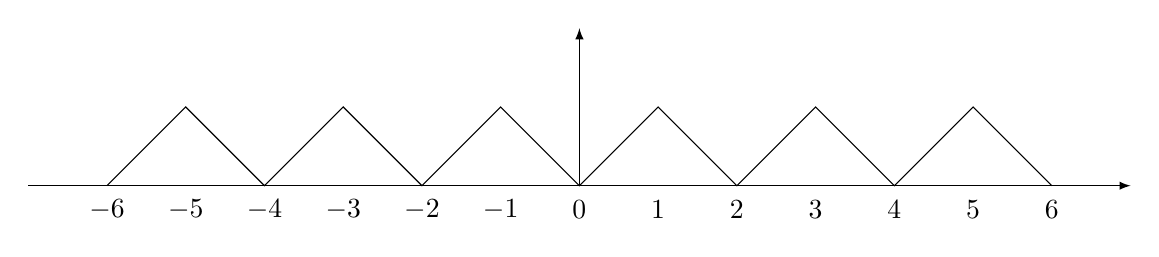
\begin{tikzpicture}
		\draw[-latex] (-7,0) -- (7,0);
		\draw[-latex] (0,0) -- (0,2);
		\draw (-6,0) -- (-5,1) -- (-4,0) -- (-3,1) -- (-2,0) -- (-1,1) -- (0,0) -- (1,1) -- (2,0) -- (3,1) -- (4,0) -- (5,1) -- (6,0);
		\draw (-6,-0.3) node{$-6$};
		\draw (-5,-0.3) node{$-5$};
		\draw (-4,-0.3) node{$-4$};
		\draw (-3,-0.3) node{$-3$};
		\draw (-2,-0.3) node{$-2$};
		\draw (-1,-0.3) node{$-1$};
		\draw (0,-0.3) node{$0$};
		\draw (1,-0.3) node{$1$};
		\draw (2,-0.3) node{$2$};
		\draw (3,-0.3) node{$3$};
		\draw (4,-0.3) node{$4$};
		\draw (5,-0.3) node{$5$};
		\draw (6,-0.3) node{$6$};
	\end{tikzpicture}
	\caption{Graph of $\phi$}
\end{figure}

	Define $f_n(x) = \left(\frac{3}{4}\right)^n \phi(4^n x)$.
	Then $|f_n| \le \left(\frac{3}{4}\right)^n$.
	By Weierstrass M test, $\displaystyle \sum_{n = 0}^\infty f_n$ converges uniformly on $\mathbb{R}$.
	Consider the function $f : \mathbb{R} \to \mathbb{R}$ defined by $\displaystyle f(x) = \sum_{n = 0}^\infty \left(\frac{3}{4}\right)^n \phi(4^n x)$.
	This sum function $f$ is continuous since the convergence is uniform and $f_n$ are all continuous.\\

	Fix a real number $x$ and a positive integer $m$.
	Define $\displaystyle \delta_m = \pm \frac{1}{2}\ 4^{-m}$ such that no integer lies between $4^m x$ and $4^m(x+\delta_m)$.
	This is possible since $|4^m (x+\delta_m) - 4^m x| = |4^m \delta_m| = \frac{1}{2}$.\\

	\begin{commentary}
		The choice of sign of $\delta_m$ is made depending on the value of $4^m x$.
		Suppose $x = 1.1$ and $m = 3$.
		Then $4^m x = 70.4$.
		Now $\delta = \frac{1}{2}\ 4^{-m} = \frac{1}{128}$ so that $4^m(x+\delta_m)= 70.9$.
		Suppose $x = 1.2$ and $m = 3$.
		Then $4^m x = 76.8$.
		Now $\delta = -\frac{1}{2}\ 4^{-m} = -\frac{1}{128}$ so that $4^m(x+\delta) = 76.3$.\\
	\end{commentary}

	Define
	\[\gamma_n = \frac{\phi(4^n(x+\delta_m)) - \phi(4^n x)}{\delta_m} \]

	If $n > m$, then $4^n \delta_m$ is an even integer and $\gamma_n = 0$.\\
	If $n \le m$, then 
	\[ |\gamma_n| = \left|\frac{\phi(4^n(x+\delta_m)) - \phi(4^n x)}{\delta_m} \right| \le \frac{4^n \delta_m }{\delta_m} \le 4^n \]
	since $|\phi(s)-\phi(t)| \le |s-t|$.\\
	In particular, if $n = m$, then
	\[ |\gamma_m| = \left| \frac{\phi(4^m(x+\delta_m))-\phi(4^m x)}{\delta_m} \right| = 4^m \]
	since $|\phi(4^m (x+\delta_m)) - \phi(4^m x)| = |4^m \delta| = \frac{1}{2}$ as there are no integers between $4^m(x+\delta_m)$ and $4^m x$.\\

	From the definition of $\gamma_n$ we have,
	\begin{align*}
	 \left| \frac{f(x+\delta_m) - f(x)}{\delta_m} \right| 
		& = \left| \sum_{n = 0}^m \left( \frac{3}{4} \right)^n \gamma_n \right| \\
		& = \left| 3^m + \sum_{n = 0}^{m-1} \left( \frac{3}{4} \right)^n \gamma_n \right| \\
		& \ge 3^m - \sum_{n = 0}^{m-1} 3^n = \frac{3^m+1}{2}
	\end{align*}
	Therefore, the function $f$ is not differentiable at $x$ since the following limit does not exist as $m \to \infty$.
	\[ \lim_{\delta_m \to 0} \left| \frac{f(x+\delta_m) - f(x)}{\delta_m} \right| \ge \lim_{m \to \infty} \frac{3^m+1}{2} \]
	Since the choice of $x$ is arbitrary, the function $f$ is nowhere differentiable.
\end{proof}

\pagebreak
{\Large Module 4 : Weierstrass Approximation \& Some Special Functions}
\section{Equicontinuous Family of Functions}
\begin{definition}
	Let $\sequence{f_n}$ be a sequence of functions defined on $E$.\\
	{\color{red}
	Sequence $\sequence{f_n}$ is a \textbf{bounded} sequence if every functions in the sequence is bounded.
	\[ \forall n \in N, \exists M \in \mathbb{R} \text{ such that } \forall x \in E, |f_n(x)|<M \]

	Sequence $\sequence{f_n}$ is a \textbf{pointwise bounded} sequence if there exists a function $\phi(x)$ such that $|f_n(x)| < \phi(x)$.
	In other words, sequence $\sequence{f_n}$ is a pointwise bounded sequence if $\sequence{f_n(x)}$ is bounded for every $x \in E$
	\[ \forall x \in E, \exists M \in \mathbb{R} \text{ such that } \forall n \in \mathbb{N}, |f_n(x)| < M \]
	}

	Sequence $\sequence{f_n}$ is a \textbf{uniformly bounded} sequence if there exists a real number $M$ such that $|f_n(x)| < M$ for every $x \in E$ and $n \in \mathbb{N}$.
	\[ \exists M \in \mathbb{R} \text{ such that } \forall x \in E, \forall n \in \mathbb{N}, |f_n(x)| < M \]
\end{definition}
\subsection{Two Problems}
\begin{enumerate}
	\item Whether uniform bounded sequence of uniformly bounded functions have a convergent subsequence ?
		\textbf{NO}.\\
		Sequence $\sequence{f_n}$ where $f_n(x) = \sin nx$ is uniformly bounded.
		But it doesn't have a convergent subseqeunce.
		\begin{proof}
			Suppose $\sequence{\sin nx}$ has a convergent subsequence, say $\sequence{\sin n_kx}$.
			Then by Cauchy criterion, $(\sin n_k x - \sin n_{k+1}x) \to 0$ as $n_k \to \infty$.
			\[ \lim_{n \to \infty} \sin n_k x - \sin n_{k+1}x = 0 \]
			\[ \lim_{n \to \infty} (\sin n_k x - \sin n_{k+1}x)^2 = 0 \]
			By Lebesgue dominated convergence theorem,
			\[ \lim_{n \to \infty} \int_0^{2\pi} (\sin n_kx - \sin n_{k+1}x)^2 dx = \int_0^{2\pi} \lim_{n \to \infty} (\sin n_kx - \sin n_{k+1}x)^2 dx = 0 \]
			However, the integral on the left evaluates $2\pi$ which is a contradiction.
			Clearly, the uniformly bounded sequence $\sequence{\sin nx}$ of continuous functions on compact interval $[0,2\pi]$ does not even imply existence of a subsequence which converges pointwise.
		\end{proof}
	\item Whether every uniformly bounded, convergent sequence has a  uniformly convergent subsequence ?
		\textbf{NO}.\\
		Consider,
		\[ f_n(x) = \frac{x^2}{x^2+(1-nx)^2} \]
		Sequence $\sequence{f_n}$ is a uniformly bounded sequence of functions on compact interval $[0,1]$.
		doesn't have a convergent subsequence.
		\begin{proof}
			Suppose $\sequence{f_n}$ has a convergent subsequence $\sequence{f_{n_k}} \to f$.
			Then $\displaystyle \lim_{n \to \infty} f_{n_k}(x) = f(x)$.
			We have,
			\[ \lim_{n \to \infty} f_n(x) = \lim_{n \to \infty} \frac{x^2}{x^2+(1-nx)^2} = 0 \]
			However,
			\[ \lim_{n \to \infty} f_n \left(\frac{1}{n}\right) = \lim_{n \to \infty} \frac{\left(\frac{1}{n}\right)^2}{\left(\frac{1}{n}\right)^2+0} = 1 \ne 0 = \left(\lim_{n \to \infty} f_n\right)(x) \] 
			Clearly, the sequence of functions $\{ f_n\}$ is a uniformly bounded sequence of continuous functions on a compact interval $[0,1]$.
			Therefore, uniformly bounded, convergent sequence on compact set doesn't necessarily have a uniformly convergenct subsequence.
		\end{proof}
\end{enumerate}

\begin{definition}
	Let $E$ be a subset of a metric space $X$.
	A family $\mathscr{F}$ of complex functions on $E$ is \textbf{equicontinuous} if for any $\varepsilon > 0$, there exists $\delta > 0$ such that $|f(x)-f(y)| < \varepsilon$ whenever $d(x,y) < \delta$ for any $x,y \in E$ and $f \in \mathscr{F}$.
	\[ \forall \varepsilon > 0, \exists \delta > 0 \text{ such that } \forall f \in \mathscr{F}, |f(x)-f(y)| < \varepsilon \text{ whenever } d(x,y) < \delta \]
	\begin{commentary}
		In equicontinuity, the choice of $\delta$ is independent of the choice of $f$.
	\end{commentary}
\end{definition}

\begin{theorem}
	If $\sequence{f_n}$ is a sequence of pointwise bounded, complex functions on countable set $E$, then it has a subsequence $\sequence{f_{n_k}}$ such that $\sequence{f_{n_k}(x)}$ converges for every $x \in E$.
\end{theorem}
\begin{proof}
	Let $E$ be a countable set.
	Let $\sequence{f_n}$ be a sequence of pointwise bounded, complex functions.
	Let $\sequence{x_i}$ be a sequence in $E$.
	Then $\sequence{f_n(x_1)}$ is a bounded sequence of complex numbers.
	By Bolzano-Weierstrass theorem,  $\sequence{f_n(x_1)}$ has a subsequence $S_1$, say $\sequence{f_{1,k}(x_1)}$ which converges at $x_1 \in E$.
	\[ S_1 : f_{1,1}\ f_{1,2}\ f_{1,3} \dots \]

	Consider, the subsequence $\sequence{f_{2,k}(x_2)}$ of the sequence $\sequence{f_n(x_2)}$ with the same values for $k$ as in subsequence $\sequence{f_{1,k}(x_2)}$.
	Again, $\sequence{f_{2,k}(x_2)}$ is a bounded complex sequence.
	And by Bolzano-Weierstrass theorem, $\sequence{f_{2,k}(x_2)}$ has a convergent subsequence $S_2$, say $\sequence{f_{2,k'}(x_2)}$ which is a subsequence of $\sequence{f_2(x_2)}$.
	And more importantly, $S_2$ is a subsequence of $S_1$ such that $S_2$ converges for both $x_1,x_2 \in E$.
	\[ S_2 : f_{2,1}\ f_{2,2}\ f_{2,3} \dots \]

	Continuing like this, we get a sequence of subsequences
	\begin{align*}
		S_1 \quad & : f_{n,1}\quad f_{n,2}\quad f_{n,3}\quad \dots \\
		S_2 \quad & : f_{n,1}\quad f_{n,2}\quad f_{n,3}\quad \dots \\
		 & \dots \\
		S_n \quad & : f_{n,1}\quad f_{n,2}\quad f_{n,3}\quad \dots
	\end{align*}

	Consider the diagonal sequence, $S : f_{1,1}\ f_{2,2}\ f_{3,3} \dots $.
	We know that discarding finitely many first terms won't affect convergence of sequences.
	And for any natural number $n$, we have can obtain a subsequence of $S_n$ by discarding a finite number of first terms from $S$.
	Thus, we have sequence $S$ which converges for $x_1,x_2,\dots,x_n \in E$ since $S_n$ converges.
	Therefore, as $n \to \infty$ we have a convergent subsequence $S$ of $\sequence{f_n}$ which converges for every $x \in E$.
\end{proof}

\begin{theorem}
	Let $K$ be a compact metric space.
	If $\sequence{f_n}$ is a sequence of pointwise bounded, continuous, complex valued functions on $K$ converges uniformly on $K$, then $\sequence{f_n}$ is equicontinuous on $K$.
\end{theorem}
\begin{proof}
	Let $K$ be a compact metric space.
	Let $\varepsilon > 0$.
	Let $\sequence{f_n}$ converges uniformly on $K$.
	Then,
	\[ \forall \varepsilon > 0,\ \exists N \in \mathbb{N} \text{ such that } \forall n > N,\ \forall x \in K,\ \| f_n(x)-f_N(x) \| < \varepsilon \]

	We have continuous functions on compact sets are uniformly continuous.
	Thus for any $\varepsilon > 0$ there exist $\delta > 0$ such that $|f_j(x) - f_j(y)| < \varepsilon$ whenever $d(x,y) < \delta$.
	Thus, $|f_N(x) - f_N(y)| \le \varepsilon$.\\

	Let $1 \le j \le N$.
	Since the continuity is uniform, there exists $\delta > 0$ such that $|f_j(x) - f_j(y)| < \varepsilon$.\dag\footnote{
		For each functions $f_j$, given $\varepsilon > 0$, there exists $\delta_j > 0$ satisfying the $\varepsilon$-$\delta$ condition for uniform continuity.
		Define $\delta = \min \{ \delta_j : j = 1,2,\dots,N \}$, then for this $\delta$ the condition is satified by functions $f_1,f_2,\dots,f_N$.}\\

	Let $n > N$ and $d(x,y) < \delta$.
	Then,
	\[ |f_n(x)-f_n(y)| \le |f_n(x)-f_N(x)| + |f_N(x) - f_N(y)| + |f_N(y) - f_n(y)| < 3\varepsilon \]

	Therefore, for any $\varepsilon > 0$ there exists $\delta > 0$ such that $\forall n \in \mathbb{N},\ |f_n(x) - f_m(x)| < \varepsilon$ whenever $d(x,y)< \delta$.
	\[ \forall \varepsilon > 0,\ \exists \delta > 0,\ \forall n \in \mathbb{N},\!\! \underset{d(x,y) < \delta}{\forall} \!\!\!\! y \in K,\ |f_n(x)-f_n(y)| < \varepsilon \]
	That is, the sequence $\sequence{f_n}$ is equicontinuous on $K$.
\end{proof}

\begin{theorem}
	Let $K$ a compact.
	If $\sequence{f_n}$ be a sequence of pointwise bounded, equicontinuous, complex functions on $K$, then
	\begin{enumerate}
		\item $\sequence{f_n}$ is uniformly bounded on $K$.
		\item $\sequence{f_n}$ has a uniformly convergent subsequence.
	\end{enumerate}
\end{theorem}
\begin{proof}
	Let $\sequence{f_n}$ be sequence of point-wise bounded, equicontinuous, complex functions on compact set $K$.
	Since $f_n$ are equicontinuous, given $\varepsilon > 0$, there exists $\delta > 0$ such that $\forall n \in \mathbb{N},\ |f_n(x)-f_n(y)| < \varepsilon$ whenever $d(x,y) < \delta$.\\

	Let $\mathcal{C}$ be a cover of $K$ of open balls of radius $\delta$.
	Since, $K$ is compact this cover has a finite subcover, say open balls with center $p_j,\ j = 1,2,\dots,r$.
	Thus there exists finitely many points, $p_j$ such that every point in $K$ is sufficiently close one of them.
	Then for any $x \in K$, there exists some $p_j$ such that $d(x,p_j) < \delta$.\\

	Since $\sequence{f_n}$ is point-wise bounded, there exists $M_j$ such that $|f_n(p_j)| < M_j$.
	Define $M = \max \{ M_1, M_2, \dots, M_r\}$. 
	Then 
	\begin{align*}
		|f_n(x)| & = |f_n(x)-f_n(p_j)+f_n(p_j)| \\
		& \le |f_n(x) - f_n(p_j)| + |f_n(p_j)| \\
		& \le \varepsilon + M
	\end{align*}
	Therefore, $\sequence{f_n}$ is uniformly bounded.\\

	\hrule \vspace{1em}

	Let $\varepsilon > 0$.
	Choose $\delta > 0$ such that $|f_n(x)-f_n(y)| < \varepsilon$ whenever $d(x,y) < \delta$.
	Since $K$ is compact, $K$ has a countable dense subset, say $E = \{x_1,x_2,\dots\}$.
	That is, given $\delta > 0$, for any $x \in K$, there exists $x_j \in E$ such that $d(x,x_j) < \delta$.
	Clearly, $K$ has a cover of open balls with center $x_j$s and radius $\delta$.
	Since $K$ is compact, there exists finitely many points $x_1,x_2,\dots,x_m \in E$ such that $d(x,x_m) < \delta$.\\

	Since $E$ is countable and $\sequence{f_n}$ is point-wise bounded, $\sequence{f_n}$ on $E$ has a subsequence, say diagonal sequence $f_{n_i} = g_i$ which converges for any $x_j \in E$.
	Thus, by Cauchy criterion there exists integer $N$ such that 
	\[ \forall i,j \ge N,\ |g_i(x_s) - g_j(x_s)| < \varepsilon,\quad s = 1,2,\dots,m \]

	Let $x \in K$.
	Let $x_s \in E$ such that $d(x,x_s) < \delta$.
	Then,
	\[ |g_i(x) - g_j(x)| \le |g_i(x)-g_i(x_s)| + |g_i(x_s) - g_j(x_s)| + |g_j(x_s) - g_j(x)| \le 3\varepsilon \]
	That is, $\sequence{g_i}$ is uniformly convergent on $K$.
	Therefore, $\sequence{f_n}$ has a uniformly convergent subseqeunce $\sequence{f_{n_k}}$.
\end{proof}

\begin{theorem}[Weierstrass' Theorem]
	If $f$ is a continuous, complex function on $[a,b]$, there exists a sequence of polynomials $P_n$ such that
	\[ \lim_{n \to \infty} P_n(x) = f(x) \]
	uniformly on $[a,b]$.
	If $f$ is real, the $P_n$ may be taken real.
\end{theorem}
\begin{important}
In other words, any continuous function has a polynomial approximation.
\end{important}
\begin{proof}
	Without loss of generality, suppose $[a,b] = [0,1]$ and $f(0) = f(1) = 0$.\\

	\textbf{Step 1 : WLoG $f(0) = f(1) = 0$}
	\begin{commentary}
	If theorem is true for continuous functions satisfying $f(0) = f(1) = 0$, then it is true for any continuous function.\\
	\end{commentary}

	Let $f$ be any continuous function on $[0,1]$.
	Then there exists a function $g : [0,1] \to \mathbb{R}$ be defined by,
	\[ g(x) = f(x)-f(0) - x[f(1) - f(0)] \]
	such that $g(0) = g(1) = 0$.
	Suppose $g$ can be expressed as limit function of a uniformly convergent sequence of polynomials, say $P_n$.
	We have,
	\[ (f-g)(x) = x[f(1) - f(0)] + f(0) \]
	is a polynomial, say $P(x)$.
	Then $P_n+P \to f$ uniformly as $n \to \infty$, since $P_n \to g$ uniformly and $P$ is a constant polynomial independent of $n$.
	\[ \lim_{n \to \infty} (P_n+P)(x) = \lim_{n \to \infty} P_n(x) + P(x) = g(x) + (f-g)(x) = f(x) \]
	Therefore, it is enough to prove the theorem is true for any continuous function $f$ satisfying $f(0) =f(1) = 0$.\\

	\hrule \vspace{1em}

	\textbf{Step 2 : Construction of $P_n(x)$}\\
	Since $f$ is continous in $[0,1]$, $f$ is uniformly continuous in $[0,1]$.
	Extend $f$ such that $f(x) = 0, \ \forall x \notin [0,1]$.
	Then,  $f$ is uniformly continuous on $\mathbb{R}$.
	Define $Q_n(x) = c_n(1-x^2)^n$ such that
	\[ \int_{-1}^1 Q_n(x) \ dx = 1 \]
	Then we have,
	\begin{align*}
		\int_{-1}^1 (1-x^2)^n \ dx 
		& = 2\int_0^1 (1-x^2)^n \ dx \ \text{ since } (1-x^2)^n \text{ is even} 
		\intertext{We have, Bernouli's inequality. $(1+x)^r \ge (1+rx),\ \forall x \ge -1,\ \forall r \ge 0$}
		\int_{-1}^1 (1-x^2)^n \ dx 
		& \ge 2\int_0^{1/\sqrt{n}} (1-nx^2) \ dx \\
		& \ge 2 \left(\frac{1}{\sqrt{n}} - \frac{n}{3n\sqrt{n}} \right) = \frac{4}{3\sqrt{n}} > \frac{1}{\sqrt{n}}
	\end{align*}
	Clearly, $c_n < \sqrt{n}$. \\

	For $\delta > 0$, $Q_n(x) \le \sqrt{n}(1-\delta^2)^n$ for $\delta \le |x| \le 1$.	
	Then $Q_n \to Q$ uniformly for all such that $\delta \le |x| \le 1$.
	Define $P_n : [0,1] \to \mathbb{R}$ defined by 
	\[ P_n(x) = \int_{-1}^1 f(x+t) \ Q_n(t) \ dt \]
	Then,
	\begin{align*}
		P_n(x) & = \int_{-1}^1 f(x+t) \ Q_n(t) \ dt \\
		& = \int_{-x}^{1-x} f(x+t) \ Q_n(t) \ dt \text{ since } f \text{ vanishes outside } [0,1]\\
		& = \int_0^{1} f(t) \ Q_n(t-x) \ dt 
	\end{align*}
	{\color{red}
	Continuous function $f$ is uniformly continuous on compact interval $[0,1]$.
	Thus $f$ is Riemann integrable on $[0,1]$.
	And $Q_n(t-x) = c_n [1-(t+x)^2]^n$.
	From integration by parts, we know that $\sequence{P_n}$ is a sequence of polynomials.
	\begin{align*}
		P_n(x) 
		& = \int_0^1 f(t) Q_n(t+x) dt \\
		& = \left[f(t)Q_n'(t+x)\right]_0^1 - \int_0^1 Q_n'(t+x) \int_0^1 f(t) dt\\
		& = f(1)Q_n'(1+x) -f(0)Q_n'(x) - [F(1)-F(0)]\int_0^1 Q_n'(t+x) dt \\
		& = f(1)Q_n'(1+x) - f(0)Q_n'(x) - [F(1)-F(0)] [Q_n(1+x) - Q_n(x)]
	\end{align*}
	}
	And for each natural number $n$, we have $P_n(x)$ is real, if $f$ is real.\\

	\hrule \vspace{1em}

	\textbf{Step 3 : $P_n \to f$ uniformly}\\
	Let $\varepsilon > 0$.
	Since extended $f$ is uniformly continuous on real line, there exists $\delta > 0$ such that $|f(y)-f(x)| < \frac{\varepsilon}{2}$ whenever $|y-x| < \delta$.
	\begin{align*}
		|P_n(x)-f(x)| 
		& = \left| \int_{-1}^1 f(x+t)Q_n(t)\ dt - f(x)\int_{-1}^1 Q_n(t)\ dt \right| \\
		& \le \int_{-1}^1 |f(x+t)-f(x)| Q_n(t)\ dt 
		\intertext{Let $M =\sup f(x)$. Then $|f(x+t)-f(x)| \le 2M$. And we have an upper bound for the value $Q_n(x)$ for $\delta \le |x| \le 1$. Therefore, we split the domain of integral into three parts so that we may apply uniform continuity on the middle part and bound of $Q_n$ on other two parts.}
		|P_n(x)-f(x)| 
		& \le 2M \int_{-1}^{-\delta} Q_n(t)dt + \frac{\varepsilon}{2} \int_{-\delta}^{\delta} Q_n(t)dt+2M\int_{\delta}^1 Q_n(t)dt 
		\intertext{We have an upper bound for $Q_n$, say $Q_n(x) \le \sqrt{n}(1-\delta^2)^n$ for $\delta \le |x| \le 1$.}
		|P_n(x)-f(x)| 
		& \le 2M\sqrt{n}(1-\delta^2)^n \int_{-1}^{-\delta} dt + \frac{\varepsilon}{2} \int_{-\delta}^{\delta} Q_n(t)dt+2M \sqrt{n} (1-\delta^2)^n \int_{\delta}^1 dt \\
		& \le 4M\sqrt{n}(1-\delta^2)^n + \frac{\varepsilon}{2} \quad \text{ since } 2(1-\delta) < 2 \\
		& \le \varepsilon \text{ for sufficiently large n}
	\end{align*}
	Therefore, there exists $N \in \mathbb{N}$ such that $\forall n > N,\ |P_n(x) - f(x)| < \varepsilon$.
	In other words, $P_n \to f$ uniformly on $[0,1]$. 
\end{proof}

\begin{corollary}
	For every interval $[-a,a]$ there is a sequence of real polynomials $P_n$ such that $P_n(0) = 0$ and
	\[ \lim_{n \to \infty} P_n(x) = |x| \]
	uniformly on $[-a,a]$.
\end{corollary}
\begin{proof}
	By Weierstrass theorem, there exists a sequence $\sequence{P_n^\ast(x)}$ of real polynomials which converges to $|x|$ uniformly on $[-a,a]$.
	Thus, $P_n^\ast(0) \to 0$ as $n \to \infty$.
	Define $P_n(x) = P_n^\ast(x) - P_n^\ast(0)$.
	Clearly, $P_n(0) = 0$ and the sequence $\sequence{P_n(x)}$ converges uniformly on $[-a,a]$.
	And,
	\[ \lim_{n \to \infty} P_n(x) = \lim_{n \to \infty} P_n^\ast(x) - \lim_{n \to \infty}P_n^\ast(0) = |x| \]	
	Therefore, $P_n(0) = 0$ and $P_n(x) \to |x|$ as $n \to \infty$.
\end{proof}

\begin{remark}[Out of Syllabus]
	On the other side of this corollary, we have Stone-Weierstrass theorem which study functions that doesn't vanish anywhere.\\

	Let $\mathscr{A}$ be an algebra of functions defined on compact set $K$ that separates points and vanishes nowhere.
	By Stone-Weierstrass theorem,\dag\footnote{
		\cite[\S7.32]{rudin} Let $\mathscr{A}$ be a family of functions defined on compact set $K$.\\
		$\mathscr{A}$ separates points if $\forall x \in K,\ \exists f,g \in \mathscr{A}$ such that $f(x) \ne g(x)$.\\
		$\mathscr{A}$ vanishes at a point $x \in K$ if $\forall x \in K,\ \exists f \in \mathscr{A}$ such that $f(x) \ne 0$ }
	any continuous function $f$ on $K$  has a sequence of functions in $\mathscr{A}$ which converges to $f$ uniformly on $K$.
	The algebra of even polynomials doesn't separate points since $P_n(x) = P_n(-x)$.
\end{remark}

%\chapter{Weierstrass Approximation \& Some Special Functions
\subsection{Some special functions}
\begin{definition}[analytic function]
	A function $f$ is (real) analytic if it can be represented by a power series.
	\[ f(x) = \sum_{j=1}^\infty c_n x^n \]
\end{definition}

\begin{remark}
	The open interval in which a power series $\sum c_n x^n$ converges is the \textbf{interval of convergence}.
\end{remark}

\begin{theorem}
	Suppose series $\sum c_n x^n$ converges for $|x| < R$.
	Suppose function $f : (-R,R)$ is defined by \[ f(x) = \sum_{n = 0}^\infty c_n x^n,\ |x| < R \]
	Then,for any $\varepsilon > 0$, the series $\sum c_n x^n$ converges uniformly on $[-R+\varepsilon,R-\varepsilon]$.
	Also the function $f$ is continuous and differentiable in $(-R,R)$ and
	\[ f'(x) = \sum_{n = 1}^\infty nc_n x^{n-1},\quad |x| < R \]
\end{theorem}
\begin{proof}
	Let $\varepsilon > 0$.
	Then for $|x| \le R - \varepsilon$ we have $|c_n x^n| \le |c_n (R-\varepsilon)^n|$.\\

	We have, 
	\[ \limsup_{n \to \infty} |R-\varepsilon| \sqrt[n]{|c_n|} = (R-\varepsilon) \limsup_{n \to\infty} \sqrt[n]{|c_n|} = 0 < 1 \]

	By raio test, the series $\sum c_n (R-\varepsilon)^n$ converges absolutely.
	By Weierstrass M test, series $\sum c_n x^n$ converges uniformly on $[-R+\varepsilon,R-\varepsilon]$.
	In the same fashion, the series $\sum nc_n x^{n-1}$ converges uniformly on $[-R+\varepsilon,R-\varepsilon]$ since $\displaystyle \limsup_{n \to \infty} \sqrt[n]{n|c_n|} = 0$.\\

	Let $x_0 \in (-R,R)$.
	Then there exists $\varepsilon > 0$ such that $x_0 \in [-R+\varepsilon, R-\varepsilon]$.
	The series $\sum n c_n x^{n-1}$ converges to $f'(x)$ uniformly on $[-R+\varepsilon,R-\varepsilon]$ and $f(x_0) = \sum c_n x_0^n$.
	Thus, $f$ is differentiable on $[-R+\varepsilon,R-\varepsilon]$ and
	\[ f'(x) = \lim_{n \to \infty} \sum_{k=1}^n k c_k x^{k-1} = \sum_{n = 1}^\infty n c_n x^{n-1} \]
	We know that $f$ is continuous at a point if it is differentiable at that point.
	Thus, $f$ is continuous on $[-R+\varepsilon,R-\varepsilon]$.
\end{proof}

\begin{corollary}
	Suppose $\displaystyle \sum_{n = 0}^\infty c_n x^n$ converges for $|x| < R$ and function $f$ is defined by $f(x) = \displaystyle \sum_{n = 0}^\infty c_n x^n$.
	Then $f$ has derivatives of all ordres, say $f^{(k)}(x)$ given by
	\[ f^{(k)}(x) = \sum_{n=k}^\infty n(n-1)\dots(n-k+1)c_n x^{n-k} \]
	In particular,
	\[ f^{(k)}(0) = k!\ c_k \]
\end{corollary}
\begin{proof}
	Let $f(x) = \sum c_n x^n$.
	Then, we have 
	\[ f'(x) = \sum_{n = 1}^\infty n c_n x^n \]
	By mathematical induction, we have
	\[ f^{(k)}(x) = \sum_{n = k}^\infty n(n-1)\dots(n-k+1) c_n x^{n-k} \]
	When $x = 0$, we get
	\[ f^{(k)}(0) = \sum_{n = k}^\infty n(n-1)\dots(n-k+1) c_n 0^{n-k} = {\color{red}k!\ c_k} \]
\end{proof}

\begin{theorem}
	Suppose $\displaystyle \sum_{n = 0}^\infty c_n$ converges.
	Define \[ f(x) = \sum c_n x^n,\quad -1<x<1 \]
	Then,
	\[ \lim_{x \to 1} f(x) = \sum_{n=0}^\infty c_n \]
\end{theorem}
\begin{proof}
	Let $s_n = c_0 + c_1 + \dots + c_n$ and $s_{-1} = 0$.
	Suppose $\sum c_n$ converges, then $s_n$ converges, say $s_n \to s$.
	Let $\varepsilon > 0$.
	Then there exists $N \in \mathbb{N}$ such that $\forall n > N,\ |s-s_n| < \frac{\varepsilon}{2}$.\\

	Also we have,
	\begin{align*}
		\sum_{n=0}^m c_n x^n
		& = \sum_{n=0}^m (s_n-s_{n-1})x^n \\
		& = \sum_{n=0}^m s_n x^n - xs_{n-1}x^{n-1} \\
		& = \sum_{n=0}^m s_nx^n - x\sum_{n=0}^{m}s_{n-1}x^{n-1} \\
		& = \sum_{n=0}^m s_nx^n - x\sum_{n=-1}^{m-1}s_nx^n \\
		& = \sum_{n=0}^{m-1} s_nx^n + s_mx^m - x\sum_{n=0}^{m-1}s_nx^n \text{ since $s_{-1} = 0$} \\
		& = (1-x)\sum_{n=0}^{m-1} s_nx^n + s_mx^m \\
		\lim_{m \to \infty} \sum_{n=0}^m c_n x_n
		& = (1-x) \lim_{m \to \infty} \sum_{n=0}^{m-1} s_nx^n + \lim_{m \to \infty} s_m x^m  \\
		f(x) & = (1-x) \sum_{n=0}^\infty s_nx^n \text{ since $s_m \to s$, $|x|<1$ and $x^m \to 0$}
	\end{align*}

	{\color{red}
	We know that,
	\[ (1-x)\sum_{n=0}^m x^n = (1-x)(1+x+x^2+\dots+x^m) = 1-x^{m+1} \]
	Thus,
	\[ \lim_{m \to \infty} (1-x)\sum_{n=0}^m x^n = \lim_{m \to \infty} 1-x^{m+1} = 1 \]
	}
	Thus,
	\begin{align*}
		|f(x) - s| 
		& = \left| (1-x)\sum_{n=0}^\infty s_nx^n - s(1-x)\sum_{n=0}^\infty x^n \right| \\
		& = (1-x) \left| \sum_{n=0}^\infty (s_n-s)x^n \right| \\
		& \le (1-x) \sum_{n=0}^\infty |(s_n-s)x^n| \\
		& \le (1-x)\sum_{n=0}^\infty |s_n-s|\ |x|^n  \\
		& {\color{red}\le (1-x)\sum_{n=0}^N |s_n-s|\ |x|^n +  \frac{\varepsilon}{2} (1-x) \sum_{n=N+1}^\infty x^n} \\
	\end{align*}
	{ \color{red}
	Let $1-x < \delta < 1$.\dag\footnote{
		In earlier version, the term $|s_n-s|$ was neglected.
		Corrected as per the seminar by Haripriya}
	\[ \lim_{x \to 1} |f(x) - s| \le \lim_{\delta \to 0} \delta \sum_{n=0}^N |s_n -s| (1-\delta)^n + \frac{\varepsilon}{2} = 0 \]
	}	
	Therefore, 
	\[ f(1) = \lim_{x \to 1} f(x) = s = \sum_{n = 0}^\infty c_nx^n \]
\end{proof}

\begin{theorem}
	Given a double sequence $\sequence{a_{ij}}$.
	Suppose that,
	\[ \sum_{j=1}^\infty |a_{ij}| = b_i \]
	and $\sum b_i$ converges.
	Then,
	\[ \sum_{i=1}^\infty \sum_{j=1}^\infty a_{ij} = \sum_{j=1}^\infty \sum_{i=1}^\infty a_{ij} \]
\end{theorem}
\begin{proof}
	\textbf{Step 1 : Construction of $f_i$}\\
	Given series $\displaystyle \sum_{j=1}^\infty |a_{ij}|$ converges to $b_i$.
	Let $E = \{ x_0,x_1,x_2,\dots \}$ be a countable set such that $x_n \to x_0$ as $n \to \infty$.
	Define sequence of functions $\sequence{f_i}$ on $E$ such that 
	\[ f_i(x_n) = \sum_{j=1}^n a_{ij},\ \forall n \in \mathbb{N} \quad \text{ and } \quad f_i(x_0) = \sum_{j=1}^\infty a_{ij} \]
	Clearly, $f_i(x_0) = b_i$ and $f_i(x_n) \to f_i(x_0)$ as $n \to \infty$.\\

	\textbf{Step 2 : $f_i$ is continuous at $x_0$}\\
	We have, $f_i(x_n) \to f_i(x_0)$.
	{\color{red}Then \dag\footnote{
		The method of contradiction was an unnecessary complication.
		Corrected as per the seminar by Mekha},
	\[ \lim_{x_n \to x_0} f_i(x_n) = \lim_{n \to \infty} \sum_{i=1}^n a_{ij} = \sum_{i=1}^\infty a_{ij} = f_i(x_0) \]
	}
	Therefore, function $f_i$ is continuous at $x_0$.\\

	\textbf{Step 3 : Construction of $g$}\\
	Given $|f_i(x)| < b_i$ and $\sum b_i$ converges.
	Thus, $\sum f_i(x)$ converges.
	Define $g : E \to \mathbb{R}$ such that
	\[ g(x) = \sum_{i = 1}^\infty f_i(x) \]
	Since $f_i$ are continuous functions defined on a countable set $E$, the convergence is uniform and the sum $g$ is continuous.
	And we have,
	\[ \lim_{n \to \infty} \lim_{m \to \infty} \sum_{i=1}^m f_i(x_n) = \lim_{x_n \to x_0} g(x_n) = g(x_0) = \lim_{m \to \infty} \sum_{i=1}^m f_i(x_0) = \lim_{m \to \infty} \lim_{n \to \infty} \sum_{i = 1}^m f_i(x_n) \]
	{\color{red}
	Therefore,
	\[ \sum_{i=1}^\infty \sum_{j=1}^\infty a_{ij} = \sum_{j=1}^\infty \sum_{i=1}^\infty a_{ij} \]
	}
\end{proof}

\begin{theorem}[Taylor]
	Suppose $f(x) = \sum c_n x^n$, the series converging in $|x| < R$.
	If $-R < a < R$, then $f$ can be expanded in a power series about the point $x = a$ which converges in $|x-a| < R-|a|$.
	And,
	\[ f(x) = \sum_{n = 0}^\infty \frac{f^{(n)}(a)}{n!} (x-a)^n,\quad |x-a| < R-|a|\]
\end{theorem}
\begin{proof}
	Suppose 
	\begin{align*}
		f(x)
		& = \sum_{n=0}^\infty c_n[(x-a)+a]^n \\
		& = \sum_{n=0}^\infty c_n \sum_{m=0}^n  \binom{n}{m} a^{n-m}(x-a)^m 
		%& = \lim_{k \to \infty} \sum_{n=0}^k c_n \sum_{m=0}^n  \binom{n}{m} a^{n-m}(x-a)^m 
		\intertext{Changing the order of summation, we may combine coefficients of $(x-a)^m$.}
		%& = \lim_{k \to \infty} \sum_{m=0}^k \sum_{n = m}^k \binom{n}{m} c_n a^{n-m} (x-a)^m \\
		& = \sum_{m=0}^\infty \sum_{n = m}^\infty \binom{n}{m} c_n a^{n-m} (x-a)^m
	\end{align*}

	Therefore, it is enough to prove that the order of summation can be changed.
	We know that the order of summation can be changed if,
	\[ \sum_{n = 0}^\infty \sum_{m = 0}^n \left| c_n \binom{n}{m} a^{n-m} (x-a)^m \right| \text{ converges} \]
	We know that,
	\[ \sum_{n = 0}^\infty \sum_{m = 0}^n \left| c_n \binom{n}{m} a^{n-m} (x-a)^m \right| = \sum_{n = 0}^\infty |c_n|\ (|x-a|+|a|)^n \]
	and it converges if $|x-a|+|a| < R-|a|$.\\

	Also we know that, if $f(x) = \sum c_n x^n$ converges in $|x|<R$, then the convergence is uniform in $[-R+\varepsilon,R-\varepsilon]$ and it is differentiable in $(-R,R)$.
	And the derivatives are given by,
	\[ f^{(m)}(a) = \sum_{n=m}^\infty \frac{n!}{(n-m)!}c_n a^{n-m} = m! \sum_{n=m}^\infty \binom{n}{m} c_n a^{n-m} \]
	Thus,
	\[ f(x) = \sum_{m = 0}^\infty \sum_{n = m}^\infty c_n\binom{n}{m} a^{n-m} (x-a)^m = \sum_{m=0}^\infty \frac{f^{(m)}(a)}{m!}(x-a)^m \]
\end{proof}

\begin{theorem}
	Suppose the series $\sum a_n x^n$ and $\sum b_n x^n$converge in the segment $S = (-R,R)$.
	Let $E$ be the set of all $x \in S$ at which
	\[ \sum_{n = 0}^\infty a_n x^n = \sum_{n = 0}^\infty b_n x^n \]
	If $E$ has a limit point on $S$, then $a_n = b_n$.
\end{theorem}
\begin{important}
	In other words, If two power series coverges to the same function in $(-R,R)$, then the series are identical.
\end{important}
\begin{proof}
	---continue---
\end{proof}

\begin{doubt}
Whether the power series representation is unique ?
\end{doubt}

\begin{theorem}
	Let $e^x$ be defined on $\mathbb{R}$.
	Then
	\begin{enumerate}
		\item $e^x$ is continuous and differentiable for all $x$.
		\item $(e^x)' = e^x$
		\item $e^x$ is a strictly increasing function
		\item $e^{x+y} = e^x e^y$
		\item $e^x \to +\infty$ as $x \to \infty$ an d $e^x \to 0$ as $x \to \infty$ and $e^x \to 0$ as $x \to -\infty$
		\item $\displaystyle \lim_{x \to \infty} x^ne^{-x} = 0$ for every $n$.
	\end{enumerate}
\end{theorem}
\begin{proof}
	Let $\displaystyle E(z) = \sum_{k=0}^\infty \frac{z^k}{k!}$.\\

	We know that,	
	\[ E(1) = \sum_{k=0}^\infty \frac{1^n}{n!} = e \quad \text{and} \quad E(0) = 1 \]

	And,
	\begin{align*}
		E(z)E(w) & = \sum_{n=0}^\infty \frac{z^n}{n!} \sum_{m=0}^\infty \frac{w^m}{m!} \\
		& = \sum_{n=0}^\infty \sum_{k=0}^\infty \frac{z^k w^{n-k}}{k!(n-k)!}  \\
		& = \sum_{n=0}^\infty \frac{1}{n!} \sum_{k=0}^\infty \binom{n}{k} z^k w^{n-k} \\
		& = \sum_{n=0}^\infty \frac{(z+w)^n}{n!} \\
		& = E(z+w)
	\end{align*}

	Then we have,
	\[ E(z)E(-z) = E(0) = 1 \]

	We $E(1) = e > 1$.
	Let $M$ be any integer.
	Then $E(M) = e^M > M$.
	Thus there exists $x \in \mathbb{R}$ such that $E(x) > M$.
	Therefore, $E(x) \to +\infty$ as $x \to +\infty$.\\

	From definition, $E(x) > 0$ for any $x > 0$.
	And for any $x < 0$, $-x > 0$ and $E(-x) > 0$.
	Therefore, $E(x) = 1/E(-x) > 0$.
	Thus, $E(z) > 0$ for any $x \in \mathbb{R}$.
	Let $\varepsilon > 0$.
	Then there exists an integer $M$ such that $\varepsilon > 1/M$.
	We know that there exists $x \in \mathbb{R}$ such that $E(x) > M$.
	Then, $0 < E(-x) = 1/E(x) < 1/M < \varepsilon$.
	Thus, $E(x) \to 0$ as $x \to -\infty$.\\

	\begin{align*}
		E'(z) & = \lim_{h \to 0} \frac{E(z+h)-E(z)}{h} \\
		& = \lim_{h \to 0} \frac{E(z)E(h) - E(z)}{h} \\
		& = E(z) \lim_{h \to 0} \frac{E(h)-1}{h} \\
		& = E(z) \lim_{h \to 0} (h+\frac{h^2}{2!}+\frac{h^3}{3!} + \dots )/ h \\
		& = E(z) 
	\end{align*}
	Thus, $E(x)$ is differentiable at every $x \in \mathbb{R}$.
	Therefore, $E(x)$ is continuous at every $x \in \mathbb{R}$.
	Thus, the function $E : \mathbb{R} \to (0,\infty)$ is strictly increasing.\\

	By mathematical induction
	\[ E(z_1 + z_2 + \dots + z_n) = E(z_1) E(z_2) \dots E(z_n) \]
	Thus,
	\[ E(n) = E(1)^n = e^n,\ \forall n \in \mathbb{N} \]
	Also we have,
	\[ E(-1) = \frac{1}{E(1)} = E(1)^{-1} = e^{-1} \]

	\[ E(-n) = E(-1)^n = \frac{1}{E(n)^n} = E(1)^{-n} = e^{-n},\ \forall n \in \mathbb{N} \]
	Thus,
	\[ E(n) = e^n,\ \forall n \in \mathbb{Z} \]

	Let $p \in \mathbb{Q}$.
	Then $p = n/m$.
	And,
	\[ E(p)^m = E(mp) = E(n) = e^n \implies E(p) = e^p,\ \forall p \in \mathbb{Q} \]

	Let $x \in \mathbb{R}$.
	Define 
	\[ E(x) = \sup_{p < x,\ p \in \mathbb{Q}} E(p) \]

	By continuity and monotonicity of $E$, we have $E(x) = e^x,\ \forall x \in \mathbb{R}$.
	Now rewriting the results, we get
	\begin{eqnarray}
		e^{x+y} &= e^x e^y \\
		\frac{d}{dx} e^x &= e^x 
	\end{eqnarray}

	We have,
	\begin{align*}
		e^x 
		& = \sum_{k=0}^\infty \frac{x^k}{k!} \\
		& > \frac{x^{n+1}}{(n+1)!} \\
		x^n e^{-x}
		& < \frac{(n+1)!}{x} \\
		\lim_{x \to \infty} x^n e^{-x} & < (n+1)! \lim_{x \to \infty} \frac{1}{x} = 0,\ \forall n \in \mathbb{N}
	\end{align*}
	Thus, $x^n e^{-x} \to 0$ as $x \to \infty$.
	As $x \to +\infty$, $e^{x} \to +\infty$ faster than any positive power $x$.
	\begin{important}
		This is no surprise since $E(1) = e > 1 = E(0)$.
	\end{important}
\end{proof}

\begin{remark}
	The function $E : \mathbb{R} \to (0,\infty)$ is a bijection.
	Thus, there exists an inverse function $L : (0,\infty) \to \mathbb{R}$ such that $E \circ L = I_{(0,\infty)}$ and $L \circ E = I_\mathbb{R}$ such that 
	\[ L(y) = \int_1^y \frac{1}{x} dx \]
	
	Furthermore, $L(x) \to +\infty$ as $x \to +\infty$ and $L(x) \to 0$ as $x \to -\infty$.
\end{remark}
\begin{proof}
	Let $u,v \in (0,\infty)$.
	Then there exists $x,y \in \mathbb{R}$ such that $E(x) = u$ and $E(y) = v$.
	Thus,
	\[ L(uv) = L(E(x)E(y)) = L(E(x+y)) = x+y \]

	Let $y = E(x)$.
	We have, $L(E(x)) = x$.
	And $L'(E(x)) E'(x) = yL'(y) = 1$ since $E'(x) = E(x) = y$.
	Thus, $L'(y) = 1/y$.\\

	From fundamental theorem for calculus,we have
	\[ \int_a^b f(t)\ dt = F(b) - F(a) \]
	where $f = F'$ on $(a,b)$.
	We have $E(x)$ is strictly monotonic and continuous, thus $L(x)$ is monotonic and continuous on $(0,\infty)$.
	And $L(x)$ is Riemann integrable on any interval $[a,b]$ subset of $(0,\infty)$.
	Put $F = L$.
	Then,
	\[ \int_a^b L'(x) dx = \int_a^b \frac{dx}{x} = L(b) - L(a) \]
	We know that $L(1) = 0$.
	Put $a = 1$  and $b = y$.
	Then, \[ L(y) = \int_1^y \frac{dx}{x} \]

	By mathematical induction,
	\[ L(x^m) = mL(x) \ \forall m \in \mathbb{N} \]
	\[ L(x) = L(x^\frac{m}{m}) = L(x^\frac{1}{m})^m = mL(x^\frac{1}{m}) \implies L(x^\frac{1}{m}) = \frac{1}{m}L(x) \]

	Thus, $x^n = E(nL(x))$ and $x^\frac{1}{m} = E(\frac{1}{m}L(x))$.
	And,
	\[ x = E(L(x)) = E(L(\frac{1}{m}x)^m) = E(mL(\frac{1}{m}x))\]
	Therefore,
	\[ x^\alpha = E(\alpha L(x)),\quad \forall x \in \mathbb{R},\ x > 0,\  \forall \alpha \in \mathbb{Q} \]
	Rewriting the relation with $\log x$ instead of $L(x)$ and $e^x$ instead of $E(x)$, we get $x^\alpha = e^{\alpha \log x}$ for any rational $\alpha$.\\

	We have,
	\[ \frac{d}{dx}x^\alpha = \frac{d}{dx} E(\alpha L(x)) = E'(\alpha L(x)) \alpha L'(x) = E(\alpha L(x)) \frac{\alpha}{x} = \alpha x^{\alpha - 1} \]
	Suppose $\alpha \ne -1$.
	For irrational values of $x$, $L(x)$ can be obtained from,
	\[ E(\alpha L(x)) = \int_1^x y^\alpha dy \]

	We have,
	\begin{align*}
		x^{-\alpha}\log x & = x^{-\alpha} \int_1^x t^{-1}\ dt \\
		& < x^{-\alpha} \int_t^x t^{\varepsilon-1}\ dt \\
		& < x^{-\alpha} \frac{x^\varepsilon -1}{\varepsilon}
	\end{align*}
	Clearly, 
	\[ \lim_{x \to +\infty} x^{-\alpha} \log x  = 0 \]
	As $x \to +\infty$, we have $\log x \to +\infty$ slower than any positive power of $x$.
\end{proof}


\begin{theorem}
	\begin{enumerate}
		\item The function $E$ is periodic with period $2\pi i$.
		\item The functions $C$ and $S$ are periodic with period $2\pi i$.
		\item If $0 < t < 2\pi$, then $E(it) \ne 1$.
		\item If $z$ is a complex number with $|z| =1$, there is a unique $t \in [0,2\pi]$ such that $E(it) = z$.
	\end{enumerate}
\end{theorem}
\begin{proof}
	Let $\displaystyle E(z) = \sum_{k=0}^\infty \frac{z^n}{n!}$.
\end{proof}

\begin{theorem}
	Suppose $a_0,a_1,\dots,a_n$ are complex numbers.
	\[ P(z) = \sum_{n=0}^\infty a_k z^k \]
	Then $P(z) = 0$ for some complex number $z$.
\end{theorem}
\begin{proof}
	---continue---
\end{proof}



\chapter{Graph Theory}
%Text Books : \cite{balakrishnan}
%Module I:
%Introduction, Basic concepts. Sub graphs. Degrees of vertices. Paths and Connectedness, Automorphism of a simple graph, line graphs, Operations on graphs, Graph Products.
%Directed Graphs : Introduction, basic concepts and tournaments.
%(Chapter 1 Sections 1.1 – 1.7( Upto 1.7.3 including ) 1.8, 1.9)
%(Chapter 1 Sections 2.1, 2.2, 2.3) (20Hours)
%Module II:
%Connectivity : Introduction, Vertex cuts and edge cuts, connectivity and edge connectivity, blocks, Cyclical edge Connectivity of a graph.
%Trees; Introduction, Definition, characterization and simple properties, centres and cancroids, counting the number of spanning trees, Cayley’s formula.
%Applications
%(Chapter 3 Sections 3.1, 3.2 , 3.3, 3.4 and 3.5 )
%(Chapter 4 Sections4.1, 4.2, 4.3, 4.4 (Up to 4.4.3 including ) and 4.5, 4.7) (25Hours)
%Module III:
%Eulerian and Hamiltonian Graphs: Introduction, Eulereian graphs,
%Hamiltonian Graphs, Hamiltonian around’ the world’ game
%Graph Colorings: Introduction, Vertex Colorings, Applications of Graph Coloring, Critical Graphs, Brooks’ Theorem
%(Chapter 6 Sections 6.1, 6.2 and 6.3 )
%(Chapter 7 Sections 7.1, 7.2 and7.3(Up to 7.3.1 including ) (20Hours)
%Module IV:
%Planarity: Introduction, Planar and Nonplanar Graphs, Euler Formula and Its Consequences, K5 and K 3,3 are Nonplanar Graphs, Dual of a Plane Graph, The Four-Color Theorem and the Heawood Five-Color Theorem .
%Spectral Properties of Graphs: Introduction, The Spectrum of a Graph, Spectrum of the Complete Graph Kn, Spectrum of the Cycle Cn,
%(Chapter 8 Sections 8.1, 8.2 , 8.3, 8.4, 8.5 and 8.6 )
%(Chapter 11 Sections 11.1, 11.2 , 11.3 and 11.4) (25Hours)

%Module 1 - \cite{balakrishnan} 1, 2
%Module 2 - \cite{balakrishnan} 3, 4
%Module 3 - \cite{balakrishnan} 6, 7
%Module 4 - \cite{balakrishnan} 8, 11
%Missing - \cite{balakrishnan} 5, 9, 10, ?

{\Large Module 1}
%\chapter{Basic Results}
\section{Basic Results}
\subsection{Introduction}
\cite{balakrishnan}
\subsection{Basic Concepts}
\begin{definition}
	A \textbf{graph} is an ordered triple $G = (V,E,I)$ where $V$ is a nonempty set of vertices, $E$ is a set of edges and $I$ is an incidence map which associates each edge with an unordered pair of vertices.
\end{definition}

\begin{description}
	\item[end vertices] Let $e$ be an edge with $I_G(e) = \{ u,v \}$. Then $u,v$ are the end vertices of $e$. We may write $e = uv$.
	\item[incident] An edge $e =uv $ said to be incident on both vertices $u$ and $v$. Then vertices $u$ and $v$ are incident on edge $e$ as well. 
	\item[parallel edges] are those edges which have same pair of end vertices.
	\item[loop] is an edge whose both end vertices are the same.
	\item[neighbour] Vertex $u$ is neighbour of vertex $v$ if $uv$ is an edge of the graph.
	\item[Open neighbourhood] $N(u)$ is the set of all neighbours of the vertex $u$.
	\item[Closed neighbourhood] $N[u] = N(u) \cup \{ u \}$.
	\item[simple] graph does not have any parallel edges or loops.
	\item[adjacent] Two vertices $u,v$ are adjacent if both $u,v$ are incident on an edge, say $uv$. Two edges are adjacent if they have a common end vertex.
\end{description}
\begin{definition}
	A graph is \textbf{finite} if both vertex set $V$ and edge set $E$ are finite. A finite graph, $G$ order, $n(G) = |V(G)|$ and size, $m(G) = |E(G)|$. Or simply $n = |V(G)|$ and $m = |E(G)|$.
\end{definition}

\begin{definition}
	A graph $G$ is \textbf{labeled} if its vertices are distinguished from one another by means of distinct labels.
\end{definition}

\begin{definition}
	Two graphs $G$ and $H$ are \textbf{isomorphic} if there exists a pair $(\phi,\theta)$ where $\phi : V(G) \to V(H)$ and $\theta : E(G) \to E(H)$ are bijections such that $I_G(e) = \{ u,v \} \iff I_H(\theta(e)) = \{ \phi(u),\phi(v) \}$.\\

	Two simple graphs $G$ and $H$ are \textbf{isomorphic} if there exists a bijection $\phi : V(G) \to V(H)$ which induced another bijection $\theta : E(G) \to E(H)$ such that $I_G(e) = \{ u,v \} \iff I_H(\theta(e)) = \{ \phi(u),\phi(v) \}$.
\end{definition}

\begin{exercise}
	Let $G$, $H$ be simple graph and let $\phi : V(G) \to V(H)$ be a bijection such that $uv \in E(G) \implies \phi(u)\phi(v) \in E(H)$. Show that $\phi$ is not an isomorphism.
\end{exercise}
	Let $G,H$ be simple graph with bijection $\phi : V(G) \to V(H)$.
	If there exists two vertices $u,v$ which are non-adjacent in $G$, but $\phi(u),\phi(v)$ are adjacent in $H$.
	Then $\phi$ is not an isomorphism.

\begin{definition}
	A simple graph is \textbf{complete} if every pair of distinct vertices are adjacent.
	A complete graph with $n$ vertices is denoted by $K_n$.
	Then $m(K_n) = \binom{n}{2} = \frac{n(n-1)}{2}$.
	A \textbf{totally} disconnected graph has no edges.
	Thus, $0 \le m \le \binom{n}{2}$.
	A graph $G$ is trivial if it has only one vertex and no edges.
\end{definition}

\begin{definition}
	A graph $G$ is \textbf{bipartite} if its vertex set can be partitioned into two nonempty sets $X$ and $Y$ such that every end of $G$ has one end in $X$ and the other end in $Y$. We write $G(X,Y)$ is bipartite with partition $X,Y$.
	A simple, bipartite graph $G(X,Y)$ is \textbf{complete bipartite} if every vertex in $X$ is adjacent to every vertex in $Y$. Let $G(X,Y)$ be a complete bipartite graph with $|X| = p$ and $|Y|=q$, then we write $K_{p,q}$. A graph of the form $K_{1,q}$ is called a \textbf{star}.
\end{definition}

\begin{remark}
	Let $G$ be a complete bipartite graph, $K_{p,q}$.
	Then it has order $n = p+q$ and size $m = pq$.
\end{remark}

\begin{definition}
Let $G$ be a graph. The complement $G^c$ of graph $G$ is the graph with same vertex set. Two vertices $u,v$ of $G^c$ are adjacent if and only if $u,v$ are non-adjacent in $G$.
	$$ V(G^c) = V(G) \quad \& \quad uv \in E(G^c) \iff uv \notin E(G) $$
\end{definition}
\begin{remark}
	We have, $(G^c)^c = G$, since ${uv \in G \iff uv \notin G^c \iff uv \in (G^c)^c}$ and $V(G) = V(G^c) = V((G^c)^c)$.
	Let $G$ be a graph of order $n$, then $E(G) + E(G^c) = E(K_n)$ as each edge of $K_n$ is either an edge of $G$ or an edge of $G^c$.
\end{remark}

\begin{definition}
	A simple graph is self-complementary if $G \cong G^c$.
\end{definition}
\begin{remark}
	The order of a self complementary graph $G$ of order $n$ is $n(n-1)/4$ since $m(G) = m(G^c)$ and $m(G) + m(G^c) = m(K_n)$.
\end{remark}

\subsection{Subgraphs}
\begin{description}
	\item[subgraph] A graph $H$ is a subgraph of $G$ if $V(H) \subset V(G)$, $E(H) \subset E(G)$ and $I_H$ is $I_G$ restricted to $E(H)$. Then $G$ is a \textbf{supergraph} of $H$.
	\item[induced subgraph] Let $G$ be a graph and $S$ be a subset of the vertex set of $G$. The subgraph induced by $S$, $G[S]$ has vertex set $S$ and two vertices are adjacent only if they are adjacent in $G$.
	\item[edge induced subgraph] Let $G$ be a graph and $S$ be a subset of the edge set of $G$. The subgraph induced by the edge set $S$ is denoted by $G[S]$. Vertex $u$ is a vertex of $G[S]$ only if $S$ has an edge incident on it.
	\item[spanning subgraph] Let $H$ be a subgraph of graph $G$. If $V(H) = V(G)$, then $H$ is a spanning subgraph.
	\item[clique] is a subgraph which is complete. A clique is maximal if it is not contained in another clique.
\end{description}

\begin{remark}
	If an edge $e$ is deleted from a graph $G$, then vertex set remains the same. The graph $G-\{e\}$ is a spanning subgraph of $G$.
	If a vertex $u$ is deleted from a graph $G$, then all the edge incident on $u$ are also deleted. The graph $G-\{u\}$ is an induced subgraph of $G$.
\end{remark}

\subsection{Degree of Vertices}
\begin{definition}
	Let $G$ be a graph and $u$ be a vertex of $G$.
	The \textbf{degree} of $u$ is the number of edges incident on it with multiplicities. That is, every loop incident on $u$ is counted twice.
\end{definition}
\begin{remark}
	In a simple graph, the degree of a vertex is the cardinality of its open neighbourhood.
	$\deg_G(u) = |N_G(u)|$.
\end{remark}

\begin{definition}
	A graph $G$ is $\mathbf{k}$-\textbf{regular} if every vertex is of degree $k$. Graph $G$ is \textbf{regular} if it is $k$-regular for some $k$. \textbf{Cubic} graphs are the $3$-regular graphs.
\end{definition}
\begin{remark}
	Complete graph $K_{n+1}$ are $n$-regular.
	And complete graphs are the smallest regular graphs.
	$K_4$ is cubic.
	Petersen graph is cubic.
\end{remark}
\begin{figure}
\centering
\scalebox{0.9}{
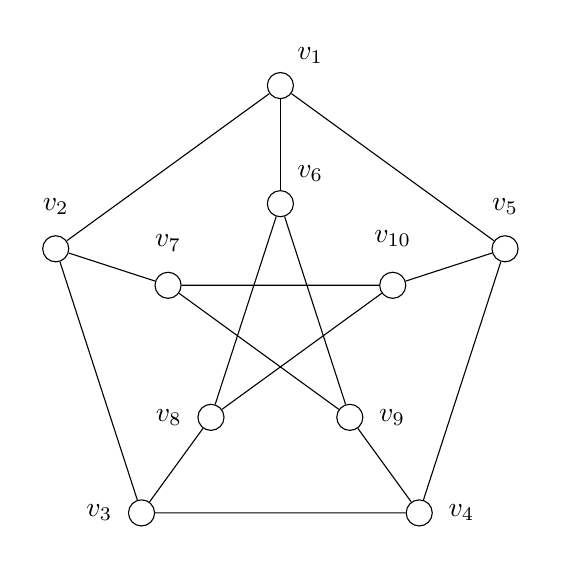
\begin{tikzpicture}
	\node (u){};
	\tikzstyle every node=[draw,circle]
	\draw (u) ++(90:1.5) node (b1)[label=above right:$v_6$]{};
	\draw (u) ++(162:1.5) node (b2)[label=above:$v_7$]{};
	\draw (u) ++(234:1.5) node (b3)[label=left:$v_8$]{};
	\draw (u) ++(306:1.5) node (b4)[label=right:$v_9$]{};
	\draw (u) ++(18:1.5) node (b5)[label=above:$v_{10}$]{};

	\draw (u) ++(90:3) node (a1)[label=above right:$v_1$]{};
	\draw (u) ++(162:3) node (a2)[label=above:$v_2$]{};
	\draw (u) ++(234:3) node (a3)[label=left:$v_3$]{};
	\draw (u) ++(306:3) node (a4)[label=right:$v_4$]{};
	\draw (u) ++(18:3) node (a5)[label=above:$v_5$]{};

	\draw (b1)--(b3)--(b5)--(b2)--(b4)--(b1);
	\draw (a1)--(a2)--(a3)--(a4)--(a5)--(a1);

	\draw (a1)--(b1);
	\draw (a2)--(b2);
	\draw (a3)--(b3);
	\draw (a4)--(b4);
	\draw (a5)--(b5);
\end{tikzpicture}
}
\end{figure}
\begin{remark}
	The complement of a regular graph is also regular. If $G$ is $k$-regular, then $G^c$ is $r$-regular where $k+r = n-1$.
\end{remark}
\begin{description}
	\item[1-factor] is a spanning, $1$-regular subgraph.
	\item[isolated vertex] is a vertex with degree $0$.
	\item[pendent vertex] is a vertex with degree $1$.
	\item[pendent edge] is the only edge incident on a pendent vertex.
\end{description}

\begin{theorem}[Euler]
	The degree sum of a graph is twice its size.
\end{theorem}
\begin{proof}
	Every edge $e= uv$ contributes $1$ to the degree of both the end vertices $u$ and $v$. Thus every edge contributes $2$ to the degree sum. There are $m$ edges, thus degree sum is $2m$.
\end{proof}

\begin{corollary}
	In a grpah $G$, the number of vertices of odd degree is even.
\end{corollary}
\begin{proof}
	Let $G$ be a graph of order $n$.
	Let $V_1,V_2$ be the set of vertices of even,odd degree respectively.
	Then, $\sum d_i = \sum_{v \in V_1} \deg(v) + \sum_{v \in V_2} \deg(v)$.
	The degree sum is even and the first sum on RHS is also even. Thus the second sum should be even. Since, each term in the second sum is an odd integer, there are even number of terms in the second sum. In other words, there are even number of vertices with an odd degree.
\end{proof}
\begin{exercise} 
	If $G \overset{\phi}{\cong} H$, then each pair $u,\phi(u)$ have the same degree.
\end{exercise}
Let $G,H$ be isomorphic graphs.
Let $u$ be a vertex of $G$.
A vertex $v$ is adjacent of $u$ in $G$ if and only if $\phi(v)$ is adjacent to $\phi(u)$ in $H$. Thus, $\deg_G(u) = \deg_H(\phi(u))$.

\begin{remark}
	Clearly, a graph isomorphism preserves adjacency, degree of vertices and neighbourhoods, etc.
	$N_H(\phi(u)) = \{ \phi(v) : v \in N_G(u) \}$.
\end{remark}

\begin{exercise}
	Let $d : d_1,d_2,\dots,d_n$ be the degree sequence of a graph $G$.
	Let $r$ be a positive integer, then $\sum d_i^r$ is even.
\end{exercise}
Let $G$ be a graph of order $n$.
Let $V_1,V_2$ be the set of vertices of even and odd degree respectively.
Clearly, $\sum d_i^r = \sum_{v \in V_1} d_i^r + \sum_{v \in V_2} d_i^r$.
Once again, the first sum on RHS is even as $d_i^r$ is even when $d_i$ is even. And the second sum is odd as $d_i^r$ is odd when $d_i$ is odd. By Euler's theorem, there are an even number of such odd terms. Thus, the second sum on RHS is also even. Therefore, $\sum d_i^r$ is even.

\begin{definition}
	A sequence of nonnegative integers $d : d_1,d_2,\dots,d_n$ is \textbf{graphical} if there exists a \textit{simple} graph with degree sequence $d$.
\end{definition}

\begin{example}
	The sequence $d : 7,6,3,3,2,1,1,1$ is nongraphical. Let $v_0,v_1$ be the vertics with degree $7,6$ respectively. Then for $d$ to be graphical, there should be at least another $4$ vertices with degree greater than or equal to $2$.
	This is not the case, therefore $d$ is not graphical.
\end{example}

\begin{exercise}
	Let $d : d_1,d_2,\dots,d_n$ is a sequence of nonnegative integers with $\sum d_i$ even. Show that there exists a non-simple graph with $d$ as its degree sequence.
\end{exercise}
	Let $d : d_1,d_2,\dots,d_n$ be a sequence of nonnegative integers with $\sum d_i$ even. Then there are even number of odd integers (if any).\\

	Step 1 : Draw a vertex $u_i$ for each term $d_i$.
	If a pair $(d_i,d_j)$ is odd\footnote{If you want maximal simple graph, you may add an edge $u_iu_j$(if it not already there) and subtract $1$ from both $d_i$ and $d_j$, provided both $d_i$ and $d_j$ are nonzero.}, then draw an edge $u_iu_j$ and subtract $1$ from both $d_i$ and $d_j$.\\

	Step 2 : If $d_i = 2k$. Draw $k$ loops on $u_i$.\\

\begin{challenge}
	Draw maximal connected graph for a degree sequence ?
\end{challenge}

\begin{application}
	In any group of $n$ persons ($n \ge 2$), there are at least two with same number of friends.
\end{application}
\begin{proof}
	Suppose group of $n$ persons is modelled by a graph with $n$ vertices and two vertices are adjacent if the respective persons are friends. It is assumed that friendship is mutual, otherwise it is not considered. Suppose all of them have different number of friends. Then every vertex in the graph has different degree.\\

	The possible degree of a vertex in a graph of order $n$ is $0,1,\dots,(n-1)$. Since all $n$ vertices have different degree and we have only $n$ options. There exists a vertex of degree $j$ for each $0 \le j < n$. This leads to a contradiction.\\

	Let $v_1,v_n$ be the vertices with degree $0,(n-1)$. Then $v_n$ is adjacent to every other vertex and $v_1$ is non-adjacent to every other vertex which is not possible. Thus, at least two vertices should have same degree. Therefore, in a group of $n$ persons, at least two of them have same number of friends.
\end{proof}

\begin{exercise}
	Let $G$ be a graph in which every vertex is of degree $k$ or $k+1$. Then the number of vertices with degree $k$ is $(k+1)n-2m$.
\end{exercise}
\begin{proof}
	Let $G$ be a graph of order $n$ and size $m$.
	Let $x$ be the number of vertices with degree $k$.
	Then there are $n-x$ vertices with degree $k+1$.
	By Euler's theorem, $ xk + (n-x)(k+1) = 2m \implies x = (k+1)n-2m$.
\end{proof}
	
\subsection{Paths and Connectedness}
\begin{definition}
	Let $G$ be a graph. A \textbf{walk} on $G$ is an alternating finite sequence of vertices and edges which starts and ends at some vertices, say $W : v_0 e_0 v_1 e_1 \dots e_k v_k$.
	The vertex $v_0$ is the \textbf{origin} and $v_k$ is the \textbf{terminus} of the walk $W$.
\end{definition}
\begin{description}
	\item[closed walk] A walk is \textbf{closed} if its origin and terminus are identical. Otherwise the walk is \textbf{open}.
	\item[trail] is a walk in which edges are distinct.
	\item[path] is a trail in which vertices are distinct.
	\item[cycle] is a closed trail in which vertices are distinct.
\end{description}

\begin{remark}
	A walk of length zero is a single vertex. And this walk is called a \textbf{trivial path}.
	Let $P : v_0,e_1,v_1,e_2,v_2,\dots,v_{k-1},e_k,v_k$ be a path in $G$. Then the \textbf{inverse of the path} is given by, $P^{-1} : v_k,e_k,v_{k-1},\dots,v_1,e_1,v_0$.
	And $v_j,e_j,v_{j+1},\dots,v_{k-1},e_{k-1},v_k$ is the $v_j-v_k$ \textbf{section} of the path $P$.
\end{remark}

\begin{definition}
	Let $G$ be a graph. Then connectedness is an equivalence relation on $V(G)$. Let $V_1,V_2,\dots,V_\omega$ be the equivalence classes. Then the induced subgraphs $G[V_1], G[V_2], \dots, G[V_\omega]$ are the \textbf{components} of $G$.
\end{definition}

\begin{remark}
	For a connected graph, $\omega = 1$. And for disconnected graphs $\omega \ge 2$. And components are maximal connected subgraphs of $G$. The number of components of $G$ is denoted by $\omega(G)$.
\end{remark}

\begin{definition}
	Let $d : V(G) \to V(G),\ d(u,v)$ is the length of the shortest $u-v$ path. If there is no $u-v$ path, then $d(u,v) = \infty$.
\end{definition}
\begin{exercise}
	Let $G$ be a simple graph.
	The vertex set $V(G)$ together with distance function $d(u,v)$, length of shortest $u-v$ path is a metric space.
\end{exercise}
\begin{proof}
	Let $G$ be a simple graph with vertex set $V(G)$ and $d : V(G) \to V(G),\ d(u,v)$ is the length of a shortest $u-v$ path.
\begin{enumerate}
	\item Every path has non-negative length. Thus, $\forall u,v \in V(G),\ d(u,v) \ge 0$.\\
	And $d(u,u) = 0$ since trivial path has zero length.
	\item Suppose $u,v$ are connected in $G$. Otherwise $d(u,v) = d(v,u) = \infty$.\\
	Let $P$ be a shortest $u-v$ path. Then $P^{-1}$ is a shortest $v-u$ path.
	Suppose there exists a $v-u$ path, $Q$ which is shorter than $P^{-1}$. Then $Q^{-1}$ is shorter than $P$ which is a contradiction.
	Thus, $d(u,v) = d(v,u)$.
	\item Suppose $d(u,v) < \infty$. Otherwise the result is trivial.\\
	Let $P,Q$ be shortest $u-w$ path, $w-v$ path in $G$. Then $P+Q$ is a $u-v$ walk.
	Thus, there exists a $u-v$ path\footnote{Every $u-v$ walk, contains a $u-v$ path which can be obtained by subsequently replacing each $w-w$ section of the walk with $w$.} of length less than or equal to the length of $P+Q$.
	Therefore, $d(u,v) \le d(u,w) + d(w,v)$.
\end{enumerate}
\end{proof}

\begin{proposition}
	If $G$ is a simple graph with $\delta(G) \ge \frac{n-1}{2}$, then $G$ is connected.
\end{proposition}
\begin{proof}
	Let $G$ be a graph of order $n$.
	Suppose $G$ is not connected. Then $G$ has at least two components, say $G_1$ and $G_2$.
	Let $v \in V(G_1)$. Since $\deg(v) \ge \frac{n-1}{2}$, there are at least $\frac{n-1}{2}$ other vertices in $G_1$.
	Thus, each component of $G$ has at least $\frac{n+1}{2}$ vertices.
	And $G$ has at least $\frac{n+1}{2} + \frac{n+1}{2}$ vertices which is a contradiction.
	Therefore, $G$ is connected.
\end{proof}

\begin{exercise}
	A simple graph with $\delta(G) \ge \frac{n-2}{2}$ is not necessarily connected.
\end{exercise}
\begin{proof}
	Let $G$ be a simple graph with $\delta(G) = \frac{n-2}{2}$ where $n$ is even. Then $G$ is not necessarily connected. For example, $2K_2$ has $\delta = 1$ and is disconnected.
\end{proof}

\begin{exercise}
	In a group of six people, there must be three people who are mutually acquainted or three people who are mutually nonacquainted.
\end{exercise}
\begin{proof}
	Suppose the result is not true.
	Then every person $u$ has at least one friend. Suppose $u$ has no friends. Then $(v,w,x)$ are mutual friends. Otherwise, either $(u,v,w)$, $(u,v,x)$ or $(u,w,x)$ are mutually non-acquainted.\\
	
\begin{figure}[hbt]
\centering
\scalebox{0.9}{
\begin{tikzpicture}
	\tikzstyle every node=[draw,circle]
	\node (u)[label=above:$u$]{};
	\node (v)[above right=1cm of u,label=above:$v$]{};
	\node (w)[below right=1cm of u,label=below:$w$]{};
	\node (x)[right=1cm of v,label=above:$x$]{};
	\node (y)[right=1cm of w,label=below:$y$]{};
	\node (z)[below right=1cm of x,label=above:$z$]{};
	\draw[dotted] (w)--(u)--(v);
	\draw[dotted] (x)--(u)--(y);
	\draw[dotted] (u)--(z);
	\draw[dashed,red] (v)--(w)--(z)--(v);
\end{tikzpicture}
}
\caption{Minimum Degree $\delta(G) > 0$}
\end{figure}
	There exists a person $u$ with at least two friends. Suppose every person has exactly one friend, say $(u,v), (w,x), (y,z)$ are friends. Then $(u,w,y)$ are mutually non-acquainted.\\

\begin{figure}[hbt]
\centering
\scalebox{0.9}{
\begin{tikzpicture}
	\tikzstyle every node=[draw,circle]
	\node (u)[label=above:$u$]{};
	\node (v)[above right=1cm of u,label=above:$v$]{};
	\node (w)[below right=1cm of u,label=below:$w$]{};
	\node (x)[right=1cm of v,label=above:$x$]{};
	\node (y)[right=1cm of w,label=below:$y$]{};
	\node (z)[below right=1cm of x,label=above:$z$]{};
	\draw (u)--(v);
	\draw (w)--(x);
	\draw (y)--(z);
	\draw[dotted,red] (u)--(w)--(y)--(u);
\end{tikzpicture}
}
\caption{Maximum degree $\Delta(G) > 1$}
\end{figure}
	Suppose $u$ has at least two friends, say $v,w$. Then $v,w$ are not friends, otherwise $(u,v,w)$ are mutual friends.
	Every other person $x,y$ and $z$ is friend of either $v$ or $w$. Suppose $x$ is not a friend of both $v$ and $w$. Then $(v,w,x)$ are mutually non-acquainted. Suppose $x$ is a friend of $v$ or $w$ or both. Then $u$ is not a friend of $x$. Otherwise either $(u,v,x)$ or $(u,w,x)$ are mutual friends.\\

\begin{figure}[hbt]
\centering
\scalebox{0.9}{
\begin{tikzpicture}
	\tikzstyle every node=[draw,circle]
	\node (u)[label=above:$u$]{};
	\node (v)[above right=1cm of u,label=above:$v$]{};
	\node (w)[below right=1cm of u,label=below:$w$]{};
	\node (x)[right=1cm of v,label=above:$x$]{};
	\node (y)[right=1cm of w,label=below:$y$]{};
	\node (z)[below right=1cm of x,label=above:$z$]{};
	\draw (v)--(u)--(w);
	\draw[dotted,red] (v)--(x)--(w)--(v);
\end{tikzpicture}
\hspace{2cm}
\begin{tikzpicture}
	\tikzstyle every node=[draw,circle]
	\node (u)[label=above:$u$]{};
	\node (v)[above right=1cm of u,label=above:$v$]{};
	\node (w)[below right=1cm of u,label=below:$w$]{};
	\node (x)[right=1cm of v,label=above:$x$]{};
	\node (y)[right=1cm of w,label=below:$y$]{};
	\node (z)[below right=1cm of x,label=above:$z$]{};
	\draw (v)--(u)--(w);
	\draw[dotted] (v)--(w);
	\draw[dashed,blue] (v)--(x);
	\draw[dashed,blue] (w)--(x);
	\draw[dotted] (u)--(x);
	\draw[dotted] (u)--(y);
	\draw[dotted] (u)--(z);
\end{tikzpicture}
}
\caption{$\deg_G(u) = 2$ or $\Delta(G) = 2$}
\end{figure}
	Similarly, $u$ is not a friend of $y$ and $z$. Thus, $\deg(u) = 2$. And $\Delta(G) = 2$.\\

	Suppose $(x,y,z)$ are not mutual friends. Then either $(u,x,y), (u,y,z)$, or $(u,z,x)$ are mutually non-acquainted which is a contradiction.
\begin{figure}[hbt]
\centering
\scalebox{0.9}{
\begin{tikzpicture}
	\tikzstyle every node=[draw,circle]
	\node (u)[label=above:$u$]{};
	\node (v)[above right=1cm of u,label=above:$v$]{};
	\node (w)[below right=1cm of u,label=below:$w$]{};
	\node (x)[right=1cm of v,label=above:$x$]{};
	\node (y)[right=1cm of w,label=below:$y$]{};
	\node (z)[below right=1cm of x,label=above:$z$]{};
	\draw (v)--(u)--(w);
	\draw[dotted] (v)--(w);
%	\draw[blue] (v)--(x);
	\draw[dotted,blue] (u)--(x);
	\draw[dotted,blue] (u)--(y);
	\draw[dotted,blue] (u)--(z);
	\draw[dashed,red] (x)--(y)--(z)--(x);
\end{tikzpicture}
}
\end{figure}
\end{proof}

\begin{theorem}
	If a simple graph $G$ is not connected, then $G^c$ is connected.
\end{theorem}
\begin{proof}
	Let $G$ be a disconnected graph with at least two components $G_1,G_2$.
	Let $u,v \in V(G)$. It is enough to prove that there exists a $u-v$ path in $G^c$.\\

	Case 1 : Two vertices $u,v$ belong to different components of $G$.
	Then $u,v$ are non-adjacent in $G$. Thus, $u,v$ are adjacent in $G^c$. Therefore, there exists a $u-v$ path in $G^c$.\\

	Case 2 : Suppose $u,v$ belongs to the same component of $G$. Let $w$ be a vertex from another component of $G$. Then $u,w,v$ is a $u-v$ path in $G^c$.\\

	Therefore, there exists a $u-v$ path between any pair of vertices in $G^c$.
\end{proof}

\begin{corollary}
	If a graph is self-complementary, then it is connected.
\end{corollary}
\begin{proof}
	Suppose $G$ is disconnected. Then its complement is connected. Therefore, $G$ is not self-complementary.
\end{proof}

\begin{exercise}
	Let $G$ be a self-complementary graph.\\ Then $n(G) \cong 0 \text{ or } 1 \pmod{4}$.
\end{exercise}
\begin{proof}
	Let $G$ be a self-complementary graph of order $n$.
	Then $m(G) = m(G^c)$ since $G \cong G^c$.
	And $m(G)+m(G^c)= m(K_n)$ since every edge in $K_n$ is either an edge of $G$ or an edge of $G^c$.
	We know that, $m(K_n) = n(n-1)/2$.
	Therefore, $m(G) = n(n-1)/4$.
	Since $n,n-1$ are consecutive, at most one of them is even.
	Therefore, either $n \cong 0 \pmod{4}$ or $n-1 \cong 0 \pmod{4}$.
\end{proof}

\begin{exercise}
	Let $G$ be a self-complementary graph.
	If $G$ has one pendent vertex, then it has another pendent vertex.
\end{exercise}
\begin{proof}
	Let $G$ be a self-complementary graph with isomorphism $\phi$ from $V(G)$ to $V(G^c)$.
	Let $u$ be a pendent vertex of $G$.
	Then $\phi(u)$ is also a pendent vertex of $G$.
	Suppose $u = \phi(u)$. Then, $n-1 = \deg(u) + \deg(\phi(u)) = 2$. However, no graph of order $3$ is self-complementary.
	Therefore, $u \ne \phi(u)$.
\end{proof}

\begin{exercise}
	Let $G$ be a simple graph.
	Then $m < \frac{(n-\omega)(n-\omega+1)}{2}$.
\end{exercise}
\begin{proof}
	Let $G_1,G_2,\dots,G_\omega$ be the components of $G$.
	Let $n_i,m_i$ be the order and size of $G_i$.
	Since every component is nonempty, $n-\omega+1$ is an upperbound for order of any component of $G$.
	\begin{align*}
		m 
		& \le \sum_{i=1}^\omega m_i\\
		& \le \sum_{i=1}^\omega n_i(n_i-1)/2,\quad \text{by Euler's theorem}\\
		& \le \frac{n-\omega+1}{2} \sum_{i=1}^\omega (n_i - 1),\quad \text{applying upperbound for $n_i$}\\
		& \le \frac{n-\omega+1}{2} (n - \omega)
	\end{align*}
\end{proof}

\begin{definition}
	A graph $G$ is \textbf{locally connected} at a vertex $v$ if the subgraph induced by open neighbhourhood of $v$ in $G$ is connected.
	And $G$ is locally connected if it is locally connected at every vertex.
\end{definition}

\begin{theorem}[Odd cycle characterisation of Bipartite graphs].\\
	A graph is bipartite if and only if it has no odd cycles.
\end{theorem}
\begin{proof}
	Let $G$ be a bipartite graph with partite sets $X,Y$.
	Let $C : v_0,v_1,\dots,v_k,v_0$ be a cycle in $G$.
	WLOG suppose $v_0 \in X$.
	Then $v_1 \in Y$, $v_2 \in X$, \dots.
	Clearly, if $j$ is even, then $v_j \in X$.
	Since $v_k,v_0$ are adjacent $k$ is odd and the cycle is of even length.\\

	Suppose $G$ has no odd cycles.
	Supppose $G$ is connected.
	Let $u$ be vertex of $G$.
	Define $X = \{ v \in V(G) : d(u,v) \text{ is even } \}$ and $Y = \{ v \in V(G) : d(u,v) \text{ is odd }\}$.
	Suppose vertices $v,w \in X$ are adjacent.
	Since $v,w \in X$, there exists $u-v$ path $P$ and $u-w$ path $Q$ both are of even length. Then $P+Q$ is not necessarily a $v-w$ path, let $w'$ be the last vertex they have in common. Then the $w'-v$ section of $P$, say $P'$ and $w'-w$ section of $Q$, say $Q'$ are disjoint. If $u-w'$ is of even(odd) length, then both $P',Q'$ are even(odd). And $P'+Q'+vw$ is an odd cycle which is a contradiction.\\

	Similary, if $v,w \in Y$ are adjacent then respective disjoint path $P',Q'$ are both of odd length. And $P'+Q'+vw$ is again an odd cycle which is a contradiction. Thus, $G(X,Y)$ is bipartite.\\

	Suppose $G$ is disconnected. Then each component $G_i(X_i,Y_i)$ is bipartite. And $G(X,Y)$ is bipartite where $X = \cup X_i$ and $Y = \cup Y_i$.
\end{proof}

\begin{exercise}
	Let $G$ be a simple, nontrivial graph.
	Graph $G$ is connected if and only if there exists an edge between any two nonempty partitions of $V(G)$.
\end{exercise}
\begin{proof}
	Suppose $G$ is connected.
	Let $V_1,V_2$ be two nonempty partitions of $V(G)$.
	Let $v_1 \in V_1$ and $v_2 \in V_2$.
	Then there exists a $v_1-v_2$ path, $P$ in $G$.
	Let $u$ be the first vertex in $P$ which is not from $V_1$ and $w$ be its preceeding vertex in $P$. Then $wu$ is an edge between $V_1$ and $V_2$.\\

	Suppose every nonempty parition $V_1,V_2$ has an edge between them.
	Let $u,v \in V(G)$ and $V_1 = \{ u \}$ and $V_2 = V(G)-V_1$. Then there exists an edge $uw$ between $V_1$ and $V_2$. If $w = v$, then we have a $u-v$ path. Suppose $w \ne v$. Consider $V_1 = \{u,w\}$ and $V_2 = V(G)-V_1$. Again there exists and edge between $V_1$ and $V_2$. Continuing like this, we get a $u-v$ path as the vertex set of $G$ is finite. Since every pair of vertices $(u,v)$ are connected by a $u-v$ path, the graph $G$ is connected.
\end{proof}

\begin{exercise}
	Let $G$ be a connected graph of order at least $3$.
	Then any two longest paths in $G$ has a common vertex.
\end{exercise}
\begin{proof}
	Let $G$ be a connected graph of order at least $3$.
	Let $P:u_1,u_2,\dots,u_k$, $Q : v_1,v_2,\dots,v_k$ be two longest paths in $G$ which are disjoint.
	Since $G$ is connected, there exists a $u_1-v_1$ path, $P'$ in $G$.
	Let $u_r,v_s$ be vertices in $P'$ such that $u_r-u_k$ section of $P$ and $u_r-v_1$ section of $P'$ are disjoint and $v_s-v_k$ section of $Q$ and $u_1-v_s$ section of $Q$ are disjoint. Let $P''$ be the $u_r-v_s$ section of $P'$ of length at least $1$. \\

	WLOG $u_1-u_r$ section of $P$, say $P_1$ and $v_s-v_1$ section of $Q$, say $Q_1$ are of length at least $k/2$. Then $P_1 + P''+Q_1$ is path of length at least $k/2+1+k/2$. This is a contradiction as this path is longer than the longest paths in $G$. Therefore, two longest paths in $G$ must have a common vertex.
\end{proof}

\begin{exercise}
	The union of two distinct paths joining two vertices contains a cycle.
\end{exercise}
\begin{proof}
	Let $P$, $Q$ be two distinct paths between two distinct vertices $u,v$ in $G$.
	The vertex $u$ belongs to both $P$ and $Q$.
	Let $w$ be the first vertex such that the vertex after $w$ is different in $P$ and $Q$. Let $x$ be a vertex after $w$ which is in both $P$ and $Q$. There exists such a vertex since $v$ belongs to both $P$ and $Q$. Then $w-x$ section of $P,Q$ are disjoint $w-x$ paths. Therefore, they form a cycle.
\end{proof}
\begin{exercise}
	If a simple, connected graph $G$ of order $n \ge 3$ is not complete. Then there exists three vertices $u,v,w$ such that $uv,vw$ are edges of $G$, but $uw$ is not an edge of $G$.
\end{exercise}
\begin{proof}
	Let $n \ge 3$. Since $G$ is not complete, there exists two vertices $u,v$ which are non-adjacent in $G$. Since $G$ is connected, there exists a $u-v$ path $P$ in $G$, let $w$ be the vertex preceeding $v$ in $P$. If $u,w$ are adjacent, then the proof is complete.\\

	Suppose $u,w$ are not adjacent. Rename $w$ as $v$. Again, we have a pair of vertices $u,v$ which are adjacent and a vertex $w$ preceeding $v$ on the $u-v$ path $P'$. The length of $P'$ is one less than the length of $P$. Suppose there is no such vertex for every path of length $\ge 3$. Then a $u-v$ path of length two, say $u,w,v$ has a such a vertex.
\end{proof}

\begin{definition}
	A simple graph $G$ is \textbf{highly irregular} at a vertex $v$ if all its neighbours have different degrees. A simple graph $G$ is highly irregular if it is highly irregular at every vertex of $G$.
\end{definition}
\begin{exercise}
	There does not exists highly irregular, simple connected graphs of order $3$ and $5$. 
\end{exercise}
\begin{proof}
	Let $G$ be a simple connected graph of order $3$.
	Then $G$ has a vertex $v$ with degree $2$.
	Let $u,w$ be the neighbours of $v$.
	Since $G$ is connected, degree of these vertices are $1$ or $2$.
	By Euler's theorem, the sum of degrees should be even. Therefore, the degree of $u,w$ are the same. Therefore simple connected graphs of order $3$ are not highly irregular.\\

	Let $G$ be a simple connected graph of order $5$.
	Suppose $G$ is highly irregular.
	If $G$ has a vertex $v$ with degree $4$, then the degree of its neighbours are $1,2,3$ and $4$.
	Then the degree sequence of $G$ is $4,4,3,2,1$
	This is a contradiction as $G$ has two vertices of degree $4$ and one vertex of degree $1$.
	Therefore, $G$ does not have a vertex of degree $4$.\\

	If $G$ has a vertex $v$ with degree $3$, then degree of its neighbours are $1,2,3$ as $G$ does not have a vertex of degree $0$ or $4$. By Euler's theorem, the vertex which is not adjacent to $v$ must have an odd degree.
	Therefore the degree sequence of $G$ is either $3,3,3,2,1$ or $3,3,2,1,1$.
	Let $u$ be the vertex with degree $2$. Then the neighbours $u$ of must have degree different degree say, $1$ and $3$ which is not possible as the remaining vertex needs three neighbours.\\

	Then $G$ has vertices of degree $2$ or $1$.
	By Euler's theorem, the degree sequences are $(2,1,1,1,1)$, $(2,2,2,1,1)$ or $(2,2,2,2,2)$. Clearly, not every vertex of degree $2$ have neighbours with different degree. Therefore, no graph of order $5$ is highly irregular.
\end{proof}
\begin{challenge}
	Prove that : highly irregular graphs of all orders exists, except $3,5$ and $7$.
\end{challenge}
\begin{remark}
	$P_4$ is highly irregular.\footnote{I thought, we should call it $P_3$.}
	And there exists a unique connected simple graph of order $6$ with degree sequence $3,3,2,2,1,1$ which is  highly irregular.
\end{remark}

\begin{definition}
	The \textbf{generalised Petersen graph} $P(n,k)$ is given by
	$$ V(P(n,k)) = \{ a_i,b_i : 0 \le i \le n-1 \} $$
	$$ E(P(n,k)) = \{ a_ia_{i+1}, a_ib_i, b_ib_{i+k} : 0 \le i \le (n-1) \}$$
	where the additions $i+1, i+k$ are modulo $n$.
\end{definition}
\begin{exercise}
	The generalised Petersen graph $P(n,k)$ is bipartite if $n$ is even and $k$ is odd.
\end{exercise}
\begin{proof}
	Consider the sets $X = \{ a_{2j}, b_{2j-1} : 1 \le j \le n/2 \}$ and $Y = \{ a_{2j-1}, b_{2j} : 1 \le j \le n/2 \}$. Clearly, edges of the form $a_ib_i$ has one end vertex in $X$ and other in $Y$.\\

	\textbf{Suppose $n$ is even}. Then $a_1 \in Y$ and $a_n \in X$. Therefore, edge of the form $a_i,a_{i+1}$ has one end vertex in $X$ and other in $Y$.\\

	\textbf{Suppose $k$ is odd}. If $i$ is odd, then $i+k \pmod{n}$ is even. And $b_i \in Y$ and $b_{i+k} \in X$. Similarly, if $i$ is even, then $b_i \in X$ and $b_{i+k} \in Y$. Therefore, edges of the form $b_ib_{i+k}$ has one end vertex in $X$ and other in $Y$.
	Therefore, $P(n,k)$ is bipartite if $n$ is odd and $k$ is even.
\end{proof}

\begin{exercise}
	If $G$ is simple and $\delta(G) \ge k$, then $G$ contains a path of length at least $k$.
\end{exercise}
\begin{proof}
	Let $P : v_0,v_1,\dots,v_r$ be a longest path in $G$.
	Then $v_r$ is at most adjacent to $v_1,v_2,\dots,v_{r-1}$. Otherwise, there exists a longer path in $G$.
	Therefore, $\deg(v_r) < r$. And $G$ has a vertex with minimum degree less than the length of its longest path.
	In other words, if $G$ has a vertex with minimum degree $k$ then it has a path which is at least $k$ long.
\end{proof}

\subsection{Automorphisms of a simple graph}
\begin{definition}
	An \textbf{automorphism} on a graph $G$ is an isomorphism of $G$ onto itself.
	The set $aut(G)$ is the set of all automorphisms on $G$.
\end{definition}

\begin{theorem}
	The set $aut(G)$ of all automorphisms on a simple graph $G$ together with function composition is a group.
\end{theorem}
\begin{proof}
	Let $G$ be a simple graph. Then the identity map $\phi : G \to G$ defined by $\phi(v) = v$ is a trivial automorphism on $G$. Therefore the $aut(G)$ is nonempty.\\

	We need to prove that the proposed group operation is closed. Let $\phi_1,\phi_2$ be two automorphisms on $G$. Let $u,v$ be two vertices of $G$.
	\begin{align*}
		u,v \text{ are adjacent } 
		& \iff \phi_2(u),\phi_2(v) \text{ are adjacent}\\
		& \iff \phi_1(\phi_2(u)),\phi_1(\phi_2(v)) \text{ are adjacent}
	\end{align*}
	Clearly, $\phi_1 \circ \phi_2$ are bijective and preserves adjacency and non-adjacency. Therefore, $\phi_1 \circ \phi_2$ is an automorphism. Thus, the group operation is closed.\\

	We know that function composition is associative. The trivial automorphism is the identity element of the group. And the inverse of each automorphism $\phi$ is the inverse map $\phi^{-1}$. Therefore, $\entity{aut(G),\circ}$ is a group.
\end{proof}

\begin{theorem}
	For any simple graph $aut(G) = aut(G^c)$.
\end{theorem}
\begin{proof}
	Let $G$ be a simple graph and $\phi$ be an automorphism on $G$. Let $u,v$ be two vertices of $G$.
	\begin{align*}
		u,v \text{ are non-adjacent in } G^c 
		& \iff u,v \text{ are adjacent in } G \\
		& \iff \phi(u),\phi(v) \text{ are adjacent in } G \\
		& \iff \phi(u),\phi(v) \text{ are nonadjacent in } G^c
	\end{align*}
	Clearly, every automorphism $\phi$ on $G$ is essentially a bijection on the vertex set of both $G$ and $G^c$. The $\phi$ preserves adjacency/non-adjacency of $G^c$ as well.\\

	Every autmorphism $\phi$ on $G$ is an automorphism on $G^c$.
	If $\phi \in aut(G)$ then $\phi \in aut(G^c)$. Thus, $aut(G^c) \subset aut(G)$.
	Similarly, every automorphism on $G^c$ is an automorphism on $G$ as well. 
	If $\phi \in aut(G^c)$ then $\phi \in aut(G)$. Thus, $aut(G) \subset aut(G^c)$.
	Therefore, $aut(G) \cong aut(G^c)$.
\end{proof}

\begin{exercise}
	$aut(K_n) \cong S_n$.
\end{exercise}
\begin{proof}
	Let $K_n$ be a complete graph with vertices $v_1,v_2,\dots,v_n$.
	Any automorphism $\phi$ on $K_n$ is a bijection/permutation of $n$ vertices. Thus, $\phi \in S_n$.
\end{proof}
\subsection{Line Graph}
\begin{definition}
	Let $G$ be a graph. The \textbf{line graph} of $G$ is graph $L(G)$ with vertex set in $1-1$ correspondence with edge set of $G$ and two vertices of $L(G)$ are adjacent if the corresponding edges are adjacent in $G$.
\end{definition}
\begin{commentary}
	Let $G$ be a graph with vertex set $V(G) = \{ u,v,w,x \}$ and edge set $E(G) = \{ uv, vw, wx, uw \}$. Then the line graph $L(G)$ is a graph with vertex set $V(L(G)) = \{ a,b,c,d \}$ with $1-1$ correspondence $a \to uv, b \to vw, c \to wx, d \to uw$ and edge set $E(L(G)) = \{ ab, ad, bc, bd, cd \}$ with adjacency at vertices $v,u,w,w,w$ respectively.
\end{commentary}

\subsubsection{Properties of Line graph}
Suppose $G$ has no isolated vertices.
\begin{enumerate}
	\item $G$ is connected if and only if $L(G)$ is connected.
	\begin{proof}
		Let $G$ be a connected graph. Let $e,f$ be itwo vertices of $L(G)$. Then $e,f$ corresponds to edges of $G$ say $e = uv$ and $f = wx$. Since $G$ is connected, there exists a $u-v$ path in $G$. The edges of $u-v$ path corresponds to the vertices of an $e-f$ path in $L(G)$. Therefore, two arbitrary vertices $e,f$ in $L(G)$ have a path between them. Thus, $L(G)$ is a connected graph.\\

		Let $G$ be a graph and $L(G)$ is the line graph of $G$. Suppose $L(G)$ is connected. Let $u,v$ be two vertices of $G$. Since $G$ has no isolated vertices. There exists some edges $e,f$ incident of $u,v$. Suppose $e \ne f$. Otherwise edge $uv$ is a $u-v$ path of length $1$. Since $L(G)$ is connected, there exists a $e-f$ path in $L(G)$. The vertices of $e-f$ path corresponds to edges in a $u-v$ path in $G$. Therefore, two arbitrary vertices of $G$ have a path between them. Thefore, $G$ is connected.
	\end{proof}
	\item If $H$ is a subgraph of $G$, then $L(H)$ is a subgraph of $L(G)$.
	\begin{proof}
		Let $H$ be a subgraph of $G$.
		The vertices of $L(H)$ corresponds to edges of $H$. Since $H$ is a subgraph of $G$, these edges also belong to $G$. Thus, $L(G)$ have vertices corresponding to these edges as well. In other words, $V(L(H)) \subset V(L(G))$.\\

		Two vertices in $L(H)$ are adjacent if the corresponding edges are adjacent in $H$. Clearly, these edges are adjacent in $G$ as well. Therefore, the vertices are adjacent in $L(G)$ as well. That is, $E(L(H)) \subset E(L(G))$. Therefore $L(H)$ is a subgraph of $L(G)$.
	\end{proof}
	\item The edges incident at a vertex of $G$ give rise to a clique of $L(G)$.
	\begin{proof}
		Suppose $k$ edges are incident on a vertex of $G$. Let $e_1,e_2,\dots,e_k$ be the vertices of $L(G)$ corresponding to those edges in $G$. Every pair of vertices $e_i, e_j$ among them are adjacent in $L(G)$ as the respective edges are adjacent in $G$. Thus, we have a complete subgraph of $L(G)$. Since $G$ is simple, no other edge in $G$ is simultaneously adjacent to all those edges. Therefore, the complete subgraph induced by $\{ e_1,e_2,\dots,e_k \}$ is maximal in $L(G)$.
	\end{proof}
\item Let $G$ be a simple graph. Then the degree of the vertex $e$ of $L(G)$ corresponding to an edge $e = uv$ of $G$ is given by
		$$d_{L(G)}(e) = d_G(u) + d_G(v) - 2$$
	\begin{proof}
		Let $e = uv$ be an edge in $G$. The number of edges adjacent to $e$ at $u$ is $d(u)-1$. Similarly, the number of edges adjacent to $e$ at $v$ is $d(v)-1$. Therefore, there are $d(u)+d(v)-2$ edges adjacent to $e$ in $G$. Clearly, the correpsonding vertex $e$ is adjacent to $d(u)+d(v)-2$ vertices in $L(G)$. In other words, $d_{L(G)}(e) = d_G(u)+d_G(v)-2$.
	\end{proof}
	\item Let $G$ be a simple graph with degree sequence $\mathscr{D}(G) = d_1,d_2,\dots,d_n$.
		Then size of the line graph $L(G)$ is given by $m(L(G)) = \frac{1}{2} \sum d_i^2 - m(G)$.
	\begin{proof}
	By Euler's theorem,
	\begin{align*}
		m(L(G)) 
		& = \frac{1}{2} \sum_{e \in V(L(G))} d_{L(G)}(e) \\
		& = \frac{1}{2} \sum_{e \in E(G)} \left[ d_G(u)+d_G(v)-2 \right] \\
		& = \frac{1}{2} \left[ \sum_{v \in V(G)} d_G(v)^2 \right] - m(G) 
	\end{align*}
	\end{proof}
\end{enumerate}

\begin{exercise}
	Line graph of the star $K_{1,n}$ is the complete graph $K_n$.
	$$L(K_{1,n}) \cong K_n$$
\end{exercise}
\begin{proof}
	Let $e_1,e_2,\dots,e_n$ be the edges of $K_{1,n}$.
	Clearly, $L(K_{1,n})$ has $n$ vertices.
	Since every pair of edges in $K_{1,n}$ are adjacent, the respective vertices are adjacent in $L(K_{1,n})$.
	Therefore, line graph $L(K_{1,n})$ is a complete graph with $n$ vertices, say $K_n$.
\end{proof}

\begin{exercise}
	Line graph of the cycle $C_n$ ($n \ge 3$) is $C_n$ itself.
	$$ L(C_n) = C_n$$
\end{exercise}
\begin{proof}
	Let $C_n$ be a cycle of length $n \ge 3$. Let $e_1,e_2,\dots,e_n$ be the edges of $C_n$ where $e_j,e_{j+1}$ are adjacent. Let $G$ be the line graph of $C_n$. Then $G$ has $n$ vertices corresponding to $n$ edges of $C_n$. We know that $d_{L(G)}(e) = d(u) + d(v) - 2$. Since $C_n$ are $2$-regular, $d(u) = d(v) = 2$. Then the line graph $G$ is $2$-regular. We know that, line graph of a connected graph is connected. Since $C_n$ is connected, its line graph $G$ is also connected. Since $G$ is a connected $2$-regular graph, $G$ is isomorphic to $C_n$ itself.
\end{proof}

\begin{theorem}
	Line graph of a simple graph is a path if and only if $G$ is a path.
	$$ G \cong P_n \iff L(G) \cong P_{n-1} $$
\end{theorem}
\begin{proof}
	Let $G$ be a path of length $n$, say $P_n$. Let $e_1,e_2,\dots,e_n$ be the edges of $P_n$ such that each pair of edges $e_j,e_j+1$ are adjacent except the pair $e_n,e_1$.
	\begin{commentary} (We usually consider addition modulo $n$.\end{commentary}) Then line graph $L(G)$ has $n$ vertices. Since $G$ is connected, $L(G)$ is also connected. Clearly, every vertex $e_j$ is adjacent to $e_{j+1}$ except $e_n,e_1$. Therefore, $L(P_n)$ is a path of length $n-1$, say $P_{n-1}$.\\

		Let $G$ be a simple graph with no isolated vertices. Suppose $L(G)$ is a path of length $m$, say $P_m$. By the definition of line graph the size of $G$ is $m$. Since $L(G)$ is connected, $G$ is also connected. Since $L(G)$ has two pendent vertices, $G$ has two pendent edges. Since the order of maximal subgraphs are at most $2$, the degree of vertices of $G$ is at most $2$. Therefore, $G$ is a path of length $m+1$, say $P_{m+1}$.
\end{proof}

\begin{exercise}
	\label{ex:L2G}
	Let $H = L^2(G)$ be defined as $L(L(G))$. Find $m(H)$ if $G$ is the graph in figure \ref{dia:L2G}.
\begin{figure}[hbt]
\centering
\begin{tikzpicture}
	\tikzstyle every node=[draw,circle]
	\node (u){};
	\node (v)[below=0.6cm of u]{};
	\node (w)[below left=1cm of v]{};
	\node (x)[below right=1cm of v]{};
	\node (y)[below left=1cm of w]{};
	\node (z)[below right=1cm of x]{};
	\draw (u)--(v)--(w)--(y);
	\draw (v)--(x);
	\draw (x.360) to[out=10,in=100] (z.90);
	\draw (x.270) to[out=280,in=180] (z.170);
\end{tikzpicture}
	\caption{Graph $G$ in exercise \ref{ex:L2G} }
	\label{dia:L2G}
\end{figure}
\end{exercise}
\begin{proof}
	(do it yourself)
\end{proof}

\begin{exercise}
	Show that $d_{L(G)}(uv) = d_G(u) + d_G(v)-2$ is not valid if $G$ has a loop.
\end{exercise}
\begin{proof}
	(do it yourself)
\end{proof}

\begin{exercise}
	Prove that a simple connected graph $G$ is isomorphic to its line graph if and only if it is a cycle.
\end{exercise}
\begin{proof}
	We know that the line graph of a cycle is always a cycle of same length. Thus, if $G$ is a cycle then it is isomorphic to its line graph.\\

	Let $G$ be a connected graph. Suppose $G$ is isomorphic to its line graph. Then order and size of $G$ are the same.\\

	Let $\Delta$ be the maximum degree of $G$. Then $G$ has a vertex $u$ with degree $\Delta$. Then $u$ has at least one neighbour with degree greater than $1$. Otherwise, $G \cong K_{1,\Delta}$ and $L(G) = K_{\Delta}$ is a contradiction. If degree of a vertex $v$ adjacent to $u$ has degree greater than $2$. Then $L(G)$ has a vertex $uv$ with degree greater than $\Delta$ which is a contradiction.\\

	Suppose $G$ has a vertex $u$ with $d(u) = \Delta$ and a vertex $v$ adjacent to $u$ with $d(v) = 2$. Then $L(G)$ has a vertex $x'$ with $d(x') = \Delta$ and a vertex $y'$ adjacent to $x'$ with $d(y') = \Delta-1$. Since $G \cong L(G)$. $G$ has vertices $x,y$ which adjacent and $d(x) = \Delta,\ d(y) = \Delta-1$. Then $L(G)$ has a vertex $xy$, corresponding to the edge $xy$ of $G$, with $d(xy) = 2\Delta - 3$. Clearly, $\Delta \le 3$ otherwise $L(G)$ has a vertex with degree greater than $\Delta$ which is a contradiction.\\

	Suppose $\Delta  = 3$. Then $G$ has two adjacent vertices $u,v$ with $d(u) = 3,\ d(v) = 2$. Then $L(G)$ has two adjacent vertices $x',y'$ with $d(x') = 3$ and $d(y') = 3$. Since $G \cong L(G)$, $G$ has two adjacent vertices $x,y$ with $d(x) = 3,\ d(y) = 3$. Thus $L(G)$ has a vertex $xy$ with degree $4$ which is a contradiction.\\
	
	We know that $\Delta \ne 1$, otherwise $G = K_2$ and $L(G) = K_1$ which is a contradiction. Thus, $\Delta = 2$. Since $G$ is connected, $G$ is either a path or a cycle. Suppose $G$ is a path $P_n$, then $L(G) = P_{n-1}$ which is a contradiction. Therefore $G$ is a cycle.
\end{proof}

\begin{exercise}
	Disprove : If the graph $H$ is a spanning subgraph of $G$, then $L(H)$ is a spanning subgraph of $G$.
\end{exercise}
\begin{proof}
	(do it yourself)
\end{proof}

\begin{theorem}
	If the simple graphs $G_1,G_2$ are isomorphic, then $L(G_1),L(G_2)$ are isomorphic.
\end{theorem}
\begin{proof}
	Let two simple graphs $G_1,G_2$ are isomophic.
	Then there exists an isomorphic $\phi : V(G_1) \to V(G_2)$ which gives rise to an edge set bijection $\theta : E(G_1) \to E(G_2)$ such that $\phi(u)\phi(v) = \theta(uv)$.\\

	Let $e$ be an edge of $G_1$. Then $e$ corresponds to a vertex $e$ of $L(G_1)$. By graph isomorphism, $\theta(e)$ is an edge of $G_2$ and $\theta(e)$ corresponds to a vertex $\theta(e)$ of $L(G_2)$. Consider the map $\phi' : V(L(G_1)) \to V(L(G_2))$ defined by $\phi'(e) = \theta(e)$. Clearly, $\phi'$ is a bijection.\\

	Suppose two edges $e,e'$ are adjacent in $G_1$. Then by isomorphism $\theta(e),\theta(e')$ are adjacent in $G_2$. Therefore, if two vertices $e,e'$ are adjacent in $L(G_1)$, then the respective vertices $\phi'(e),\phi'(e')$ are adjacent in $L(G_2)$. Therefore $\phi'$ is a graph isomorphism between $L(G_1)$ and $L(G_2)$. Clearly, $L(G_1) \cong L(G_2)$.
\end{proof}

\begin{remark}
	Suppose $G_1,G_2$ be simple, connected graphs. Then $L(G_1) \cong L(G_2)$ does not imply that $G_1 \cong G_2$.
\end{remark}
\begin{proof}
	Suppose $G_1 = K_{1,3}$ and $G_2 = K_3$. Then $L(G_1) \cong L(G_2) \cong K_3$ and $G_1 \not\cong G_2$.
\end{proof}

\subsection{Graph Operations}
\begin{definition}
	Let $G_1,G_2$ be two simple graph.
	Their \textbf{union} $G_1 \cup G_2$ is given by 
	$$ V(G_1 \cup G_2) = V(G_1) \cup V(G_2) \qquad E(G_1 \cup G_2) = E(G_1) \cup E(G_2) $$
	If $V(G_1) \cap V(G_2) = \phi$, then the graph $G_1 \cup G_2$ is their \textbf{sum} $G_1 + G_2$.
\end{definition}

\begin{remark}
	The finite union of graph is associative.
\end{remark}

\begin{definition}
	Let $G_1,G_2$ be two simple graph with $V(G_1) \cap V(G_2) \ne \phi$.
	Their \textbf{intersection} $G_1 \cap G_2$ is given by 
	$$ V(G_1 \cap G_2) = V(G_1) \cap V(G_2) \qquad E(G_1 \cup G_2) = E(G_1) \cap E(G_2) $$
\end{definition}

\begin{definition}
	Let $G_1,G_2$ be two vertex-disjoint graphs. Then the \textbf{join} $G_1 \vee G_2$ is the supergraph of $G_1 + G_2$ in which each vertex of $G_1$ is adjacent to every vertex of $G_2$.\\

	If $G_1 = K_1$ and $G_2 = C_n$, then $G_1 \vee G_2 \cong W_n$ a \textbf{wheel} of order $n+1$.
\end{definition}

\subsubsection{Properties of Graph Operations}
\begin{enumerate}
	\item $n(G_1 \cup G_2) = n(G_1) + n(G_2) - n(G_1 \cup G_2)$ and\\
		$m(G_1 \cup G_2) = m(G_1) + m(G_2) - m(G_1 \cup G_2)$.
		\begin{proof}
			do it yourself
		\end{proof}
	\item $n(G_1+G_2) = n(G_1) + n(G_2)$ and \\ $m(G_1+G_2) = m(G_1) + m(G_2)$.
		\begin{proof}
			do it yourself
		\end{proof}
	\item $n(G_1 \vee G_2) = n(G_1)+n(G_2)$ and \\ $m(G_1 \vee G_2) = m(G_1)+m(G_2)+n(G_1)n(G_2)$.
		\begin{proof}
			do it yourself
		\end{proof}
\end{enumerate}

\subsection{Graph Products}
\begin{definition}
	The \textbf{general graph product} $G_1 \ast G_2$ is defined as a graph with vertex set $V(G_1 \ast G_2) = V(G_1) \times V(G_2)$ and the adjacency/non-adjacency among a pair of vertices is given by the structure table $S$, 
$$ S = \begin{bmatrix} \circ & \circ & \circ \\ \circ & = & \circ \\ \circ & \circ & \circ \end{bmatrix} $$
	where $\circ$'s are either $N$ or $E$. The letter `E' means Edge and `N' means No edge.\\

	The first, second and third rows of $S$ corresponds to adjacency, equality and non-adjacency of respective vertices in $G_1$. Similarly, first, second and third columns of $S$ corresponds to adjacency, equality and non-adjacency of respective vertices in $G_2$.
\end{definition}

\begin{commentary}
	For example, $G_1,G_2$ be two simple graph given in diagram \ref{dia:generalProduct}. Let $G_1 \star G_2$ be a graph product with the following strcture table $S$ given in table \ref{tb:generalProduct}.\\

\begin{figure}[hbt]
\centering
\begin{tikzpicture}
\tikzstyle every node=[draw,black,circle]
	\node (u)[label=left:$u_1$]{};
	\node (v)[above right=1cm of u,label=left:$v_1$]{};
	\node (w)[below right=1cm of u,label=left:$w_1$]{};
	\draw[black] (v)--(u)--(w);
\end{tikzpicture}
\hfill
\begin{tikzpicture}
\tikzstyle every node=[draw,black,circle]
	\node (u)[label=above:$u_2$]{};
	\node (v)[right = 1cm of u,label=above:$v_2$]{};
	\draw[black] (u)--(v);
\end{tikzpicture}
\hfill
\begin{tikzpicture}
\tikzstyle every node=[draw,black,circle]
	\node (u1)[label=left:$u_1u_2$]{};
	\node (v1)[above right=1cm of u1,label=left:$v_1u_2$]{};
	\node (w1)[below right=1cm of u1,label=left:$w_1u_2$]{};
	\node (u2)[right=2cm of u1,label=right:$u_1v_2$]{};
	\node (v2)[above right=1cm of u2,label=right:$v_1v_2$]{};
	\node (w2)[below right=1cm of u2,label=right:$w_1v_2$]{};
%	\draw[black] (v1)--(u1)--(w1);
%	\draw[black] (v2)--(u2)--(w2);
	\draw[green] (v1)--(u1)--(w1);
	\draw[green] (w2)--(u2)--(v2);
	\draw[cyan] (u1)--(u2);
	\draw[cyan] (v1)--(v2);
	\draw[cyan] (w1)--(w2);
	\draw[blue] (v1.300) to[out=290,in=160] (w2.150);
	\draw[blue] (w1.60) to[out=70,in=200] (v2.210);
\end{tikzpicture}
	\caption{A graph product $G_1 \star G_2$}
	\label{dia:generalProduct}
\end{figure}

	For example, $v_1u_2, w_1v_2$ are two vertices of $G_1 \star G_2$. We know that $v_1,w_1$ are non-adjacent in $G_1$. Thus, we need to look at the third row of the structure table $S$. Again, $u_2,v_2$ are adjacent in $G_2$. Thus, we need to look at the first column of the structure table $S$. Clearly, $S_{3,1}$ which is $E$. Therefore, they are adjacent in $G_1 \star G_2$. Refer table \ref{tb:generalProduct} to find element of $S$ corresponding to each pair of vertices in $G_1 \star G_2$.

\begin{table}[hbt]
\centering
$ S = \displaystyle\begin{bmatrix} N & E & N \\ E & = & N \\ E & N & N \end{bmatrix}$
\hfill
\begin{tabular}{|c|c|c|c|c|c|c|} \hline
	& $u_1u_2$ & $v_1u_2$ & $w_1u_2$ & $u_1v_2$ & $v_1v_2$ & $w_1v_2$ \\ \hline
	$u_1u_2$ & $S_{2,2}$ & \textcolor{green}{$S_{1,2}$} & \textcolor{green}{$S_{1,2}$} & \textcolor{cyan}{$S_{2,1}$} & $S_{1,1}$ & $S_{1,1}$ \\ \hline
	$v_1u_2$ & \textcolor{green}{$S_{1,2}$} & $S_{2,2}$ & $S_{3,2}$ & $S_{1,1}$ & \textcolor{cyan}{$S_{2,1}$} & \textcolor{blue}{$S_{3,1}$} \\ \hline
	$w_1u_2$ & \textcolor{green}{$S_{1,2}$} & $S_{3,2}$ & $S_{2,2}$ & $S_{1,1}$ & \textcolor{blue}{$S_{3,1}$} & \textcolor{cyan}{$S_{2,1}$} \\ \hline
	$u_1v_2$ & \textcolor{cyan}{$S_{2,1}$} & $S_{1,1}$ & $S_{1,1}$ & $S_{2,2}$ & \textcolor{green}{$S_{1,2}$} & \textcolor{green}{$S_{1,2}$} \\ \hline
	$v_1v_2$ & $S_{1,1}$ & \textcolor{cyan}{$S_{2,1}$} & \textcolor{blue}{$S_{3,1}$} & \textcolor{green}{$S_{1,2}$} & $S_{2,2}$ & $S_{3,2}$ \\ \hline
	$w_1v_2$ & $S_{1,1}$ & \textcolor{blue}{$S_{3,1}$} & \textcolor{cyan}{$S_{2,1}$} & \textcolor{green}{$S_{1,2}$} & $S_{3,2}$ & $S_{2,2}$ \\ \hline
\end{tabular}
	\caption{Adjacency/Non-adjacency Table for $G_1 \star G_2$}
	\label{tb:generalProduct}
\end{table}
\end{commentary}

\begin{definition}
	The \textbf{cartesian product} $G_1 \square G_2$ is the graph product with structure table $S$ given by
	$$ S = \begin{bmatrix} N & E & N \\ E & = & N \\ N & N & N \end{bmatrix} $$
\end{definition}

\begin{definition}
	The \textbf{direct product}(tensor/Kronecker product) $G_1 \times G_2$ is the graph product with structure table $S$ given by
	$$ S = \begin{bmatrix} E & N & N \\ N & = & N \\ N & N & N \end{bmatrix} $$
\end{definition}

\begin{definition}
	The \textbf{composition product} (wreath/lexicographic product) $G_1[G_2]$ is the graph product with structure table $S$ given by
	$$ S = \begin{bmatrix} E & E & E \\ E & = & N \\ N & N & N \end{bmatrix} $$
\end{definition}

\begin{definition}
	The \textbf{strong product} (normal product) $G_1 \boxtimes G_2$ is the graph product with structure table $S$ given by
	$$ S = \begin{bmatrix} E & E & N \\ E & = & N \\ N & N & N \end{bmatrix} $$
\end{definition}

\begin{remark}
	From structure table $S$, it is evident that all the above graph products are associative and all except the composition product are commutative.
\end{remark}

\begin{challenge}
	Can you find a non-associative graph product ?
\end{challenge}

\begin{exercise}
	Show that $G_1[G_2] \not\cong G_2[G_1]$
\end{exercise}
\begin{proof}
	$K_2[K_{1,3}] \not\cong K_{1,3}[K_2]$
\end{proof}

\begin{exercise}
	Prove that $G_1 \square G_2 \cong G_2 \cong G_1$.
\end{exercise}
\begin{proof}
	Since the structure table $S$ of the cartesian graph product is symmetric the graph product is commutative.
\end{proof}

\begin{exercise}
	Prove that $G_1 \boxtimes G_2 \cong G_2 \boxtimes G_1$
\end{exercise}
\begin{proof}
	Since the structure table $S$ of the strong product is symmetric the graph product is commutative.
\end{proof}

\begin{definition}
	Let $(x,y)$ be a vertex of $G_1 \square G_2$. The $\mathbf{G_2}$ \textbf{fiber at} $\mathbf{x}$ in $G_1 \square G_2$ denoted by $(G_2)_x$ is the subgraph of $G_1 \square G_2$ induced by the set of all vertices $\{ (x,z) : z \in V(G_2) \}$. Similarly, the $\mathbf{G_1}$\textbf{-fiber at} $\mathbf{y}$, $(G_1)_y)$ is the subgraph of $G_1 \square G_2$ induced by $\{ (z,y) : z \in V(G_1) \}$.
\end{definition}


\begin{exercise}Properties of graph products
\begin{enumerate}
	\item The order of a general graph product is the product of their orders.
	\begin{align*}
		n(G_1 \square G_2) 
		= n(G_1[G_2]) = n(G_2[G_1]) & =\\
		n(G_1 \times G_2) = n(G_1 \boxtimes G_2) & = n(G_1) n(G_2)
		\end{align*}
	\begin{proof}
		The vertex set of a general graph product is the cartesian product of the vertex sets, $G_1 \ast G_2$ is $V(G_1) \times V(G_2)$. Therefore, order of a general graph product is $n(G_1)n(G_2)$.
	\end{proof}
	\item $m(G_1 \square G_2) = n(G_1) m(G_2) + m(G_1) n(G_2)$.
	\begin{proof}
		The structure table of cartesian graph product has entry $E$ at $S_{1,2}$ and $S_{2,1}$.
		Thus the edge conditions for cartesian graph product $G_1 \square G_2$ are
		\begin{enumerate*}
			\item $u_1 = v_1$ and $u_2,v_2$ are adjacent or 
			\item $u_2 = v_2$ and $u_1,v_1$ are adjacent.
		\end{enumerate*}

		\textbf{Case 1 :} Let $xy$ be an edge of $G_2$ and $v$ be a vertex of $G_1$. Then $(v,x),(v,y)$ are adjacent in $G_1 \square G_2$. Every edge of type 1 is of this form. Therefore, there are $n(G_1)m(G_2)$ edges of type $1$ in $G_1 \square G_2$.\\

		\textbf{Case 2 :} Let $xy$ be an edge of $G_1$ and $v$ be a vertex of $G_2$. Then $(x,v),(y,v)$ are adjacent in $G_1 \square G_2$. Every edge of type 2 is of this form. Therefore, there are $m(G_1)n(G_2)$ edges of type $2$ in $G_1 \square G_2$.
		Therefore, $m(G_1 \square G_2) = n(G_1)m(G_2) + m(G_1)n(G_2)$.
	\end{proof}
	\item $m(G_1[G_2]) = n(G_1) m(G_2) + n(G_2)^2 m(G_1)$.
	\begin{proof}
		The structure table for composition product has entry $E$ at first row of $S$ and $S_{2,1}$. Thus the condition for adjacency of two vertices $(u_1,u_2),(v_1,v_2)$ in $G_1[G_2]$ are
	\begin{enumerate*}
		\item $u_1,v_1$ are adjacent or
		\item $u_1 = v_1$ and $u_2,v_2$ are adjacent.
	\end{enumerate*}

		\textbf{Case 1 :} Let $xy$ be an edge of $G_1$ and $u,v$ be two vertices of $G_2$. Then an edge of type $1$ is of the form $(x,u)(y,v)$. Thus, there are $m(G_1)n(G_2)^2$ edges of type $1$ in $G_1[G_2]$.

		\textbf{Case 2 :} Let $xy$ be an edge in $G_2$ and $v$ be a vertex in $G_1$. Then an edge of type $2$ is of the form $(v,x)(v,y)$. Thus, there are $m(G_2)n(G_1)$ edges of type $2$ in $G_1[G_2]$.

		Therefore $m(G_1[G_2]) = m(G_1)n(G_2)^2 + m(G_2)n(G_1)$.
	\end{proof}
	\item $m(G_1 \times G_2) = 2m(G_1) m(G_2)$.
	\begin{proof}
		The only E entry in the structure table of direct product is $S_{1,1}$. Thus the condition for adjacency between $(u_1,u_2),(v_1,v_2)$ in $G_1 \times G_2$ is $u_1,v_1$ are adjacent and $u_2,v_2$ are adjacent.\\

		Let $uv,xy$ be edges in $G_1,G_2$ respectively. Then an edge of direct product is of the form $(u,x)(v,y)$ or $(u,y)(v,x)$. There are $m(G_1)m(G_2)$ edges of both kind.
		Therefore, $m(G_1 \times G_2) = 2m(G_1)m(G_2)$.
	\end{proof}
	\item $m(G_1 \boxtimes G_2) = n(G_1) m(G_2) + m(G_1) n(G_2) + 2m(G_1) m(G_2)$.
	\begin{proof}
		We know that the strong product is the disjoint union of the cartesian and direct graph products, $G_1 \boxtimes G_2 = G_1 \square G_2 \cup G_1 \times G_2$. 
		By the properties of sum of two graph, $E(G_1 \boxtimes G_2) = E(G_1 \square G_2) \cup E(G_1 \times G_2)$.
		Therefore, $m(G_1 \boxtimes G_2) = m(G_1 \square G_2) + m(G_1 \times G_2)$.
	\end{proof}
\end{enumerate}
\end{exercise}

\begin{exercise}
	Prove that $L(K_{m,n}) \cong K_m \square K_n$.
\end{exercise}
\begin{proof}
	Let $u_j,v_k$ be labels for the vertices of $K_m,K_n$ respectively. Abusing the language we may write that a vertex of $K_m \square K_n$ is of the form $u_jv_k$. By the definition of cartesian graph product, $u_jv_s, u_kv_t$ are adjacent if and only if $u_j,u_k$ are adjacent and $v_s,v_t$ are adjacent.\\

	Consider the line graph $L(K_{m,n})$ of the bipartite graph $K_{m,n}$ with partite set $X,Y$. Let $x_j,y_k$ be labels for vertices in the partite sets $X,Y$ respectively. The edge of $K_{m,n}$ are of the form $x_jy_k$. Two vertices $x_jy_s,x_ky_t$ are adjacent in $L(K_{m,n})$ if the respective edges have a common vertex. In other words, either $x_j = x_k$ or $y_s = y_t$.\\

	\begin{commentary}
	Define $\psi : X \to V(K_m)$ where $\psi(x_j) = u_j$ and define $\xi : Y \to V(K_n)$ where $\xi(y_k) = v_k$.
	\end{commentary}
	Define $\phi : V(L(K_{m,n})) \to V(K_m \square K_n)$ by $\phi(x_jy_k) = u_jv_k$. Clearly, $x_jy_s,x_ky_t$ are adjacent if and only if $\phi(x_jy_s)=u_jv_s$ and $\phi(x_ky_t)=u_kv_t$ are adjacent. Therefore, $L(K_{m,n}) \cong K_m \square K_n$.
\end{proof}

\begin{definition}
	The $\mathbf{k}$\textbf{th power} $G^k$ of $G$ has $V(G^k) = V(G)$ where two vertices $u,v$ are adjacent in $G^k$ whenever $d_G(u,v) \le k$.
\end{definition}

\begin{exercise}
	Show that if $G$ is a connected graph with at least two edges, then each edge of $G^2$ belongs to a triangle.
\end{exercise}
\begin{proof}
	Let $e=uv$ be an edge of $G^2$. Then there are two possibilities, either $d_G(u,v) = 1$ or $d_G(u,v) = 2$.\\

	\textbf{Case 1 :} Suppose $d_G(u,v) = 1$. Since $G$ is connected, without loss of generality there exists an edge adjacent to $uv$ at $v$, say $vw$. Then $d_G(u,w) \le 2$ and $uw \in E(G^2)$. Clearly, the edge $uv$ belongs to the triangle $\triangle uvw$ in $G^2$.\\

	\textbf{Case 2 :} Suppose $d_G(u,v)=2$. Then there exists $w \in V(G)$ such that $uw,wv \in E(G)$. Clearly, the edge $uv$ belongs to the triangle $\triangle uwv$ in $G^2$.
\end{proof}

\begin{exercise}
	If $d_G(u,v) = p$, determine $d_{G^k}(u,v)$.
\end{exercise}
\begin{proof}
	Suppose $p$ is finite. Otherwise $d_G(u,v) = \infty$ and  $d_{G^k}(u,v) = \infty$.
	Since $p,k$ are natural numbers, there exists unique integers $q,r$ such that $p = qk+r$, $q \ge 0$ and $0 \le r < k$. Then the shortest $u-v$ path contains vertices $v_1,v_2,\dots,v_q$ such that $d_G(u,v_1) = k$ and $d_G(v_j,v_{j+1}) = k$ and $d_G(v_{j+1},v) = r$. Then $u,v_1$ are adjacent in $G^k$. Similarly, $v_j,v_{j+1}$ are adjacent in $G^k$.\\

	Suppose $r = 0$. Then $v_q = v$ and $u,v_1,v_2,\dots,v_{q-1},v$ is the shortest $u-v$ path in $G^k$. Thus, $d_{G^k}(u,v) = q$. Suppose $r > 0$. Then $d_G(v_q,v) = r < k$. Thus, $v_q,v$ are adjacent in $G^k$ and $u,v_1,v_2,\dots,v_q,v$ is the shortest $u-v$ path in $G^k$. Therefore, $d_{G^k}(u,v) = q+1$.
\end{proof}

\setcounter{subsection}{11}
\subsection{Miscellaneous Exercises}
\begin{enumerate}
	\item Show that the sequences \begin{enumerate*} \item $(7,6,5,4,3,3,2)$ and \item $(6,6,5,4,3,3,1)$ are not graphical \end{enumerate*}
	\item Give an example of a degree sequence that is realizable as the degree sequence by only a disconnected graph.
	\begin{proof}[Solution]
		$(1,1,1,1)$ or $(1,1,0)$.
	\end{proof}
	\item Show that for a simple bipartite graph, $m \le n^2/4$.
	\begin{proof}[Solution]
		Let $G$ be a bipartite graph. The size of a bipartite graph is maximum when it is a complete bipartite graph with cardinality of partite set $X,Y$ almost equal.\\

		Suppose order of $G$ is even, $n = 2k$. Then the size of the bipartite graph is maximum when $p = q = k$. And size 
		$$ m \le  pq = k^2 = \frac{n^2}{4} $$
		Suppose order of $G$ is odd, $n = 2k+1$. The the size of the bipartite graph is maximum when $p = k$ and $q = k+1$. And size 
		$$ m \le pq = k(k+1) \le \left(k+\frac{1}{2}\right)^2 = \frac{n^2}{4} $$
	\end{proof}
	\item Show that $\delta \le \frac{2m}{n} \le \Delta$.
	\begin{proof}[Solution]
		By Euler's theorem, the sum of degrees of a graph is twice its size. Thus $2m/n$ is the average of the degrees of vertices. We know that, $minimum \le average \le maximum$ is true for any finite sequence.
	\end{proof}
	\item For every $n \ge 3$, construct a $3$-regular simple graph on $2n$ vertices containing no triangles.
	\begin{proof}[Solution]
		The generalised Petersen graphs $P(n,k)$ where $0 \le k \le n$ and $\gcd(n,k)=1$ are $3$-regular and does not contain any cycles.
	\end{proof}
\item If a bipartite graph $G(X,Y)$ is regular, show that $|X| = |Y|$.
	\begin{proof}[Solution]
		Since $G$ is bipartite the sum of degree of vertices both partite sets are equal, as every edge contributes one to both the sum.
		If $G$ is regular, then the degree of every vertex is the same, say $k$.\\

		Let $X,Y$ be the partite sets of $G$ with cardinality $p,q$.
		Then the degree sum of vertices in $X$ is $kp$ and the degree sum of vertices in $Y$ is $kq$.
		We know that $G$ is bipartite, thus every edge in $G$ has one end in $X$ and the other end in $Y$.
		Thus, the degree sum of $X$ and $Y$ should be the same.
		That is, $kp = kq$.
		Therefore $p = q$.
		In other word, both partite sets have the same number of vertices.
	\end{proof}
	\item Show that in a simple graph, any closed walk of odd length contains a cycle.
	\begin{proof}[Solution]
		Let $G$ be a simple graph and $W : u_0,e_1,u_1,\dots,e_n,u_0$ be a closed walk of odd length in $G$. If $W$ does not visit any vertex twice(other than the origin $u_0$), then $W$ is a cycle.\\

		Suppose $W$ visits another vertex $v$ multiple times. Suppose every such sections are of even length, then delete all those $u_j-u_k$ sections of $W$ to obtain an odd cycle contained in $W$. If the number of edges of $W$ between two consecutive visits of a vertex $v = u_j,u_k$ is odd, then $u_j-u_k$ section of $W$ is a closed walk of odd length. Repeating like this, we get an odd cycle contained in $W$.
	\end{proof}
\item Give an example of a disconnected simple graph with $\omega$ components, $n$ vertices and $\frac{(n-\omega)(n-\omega+1)}{2}$ edges
	\begin{proof}[Solution]
		Do it yourself (hint : check the proof)
	\end{proof}
\item Prove or disprove : If $H$ is a subgraph of $G$, then $\delta(H) \le \delta(G)$, $\Delta(H) \le \Delta(G)$.
	\begin{proof}[Solution]
		Do it yourself
	\end{proof}
\item If $m > \frac{(n-1)(n-2)}{2}$, then show that $G$ is connected.
	\begin{proof}[Solution]
		Check exercise $8$ with $\omega = 2$.
	\end{proof}
	\item If $\delta \ge 2$, then show that $G$ contains a cycle.
	\begin{proof}[Solution]
		Let $G$ be a graph with $\delta \ge 2$.
		Suppose $G$ doesnot contain a cycle.
		Let $v$ be a vertex of $G$ then $v$ has at least two neighbors, say $u,w$. Since $G$ has no cycles, vertices $u,w$ are non-adjacent. Then $w$ have another neighbor  $x$ and $x$ is non-adjacent to $u,v$. Thus, $x$ have another neighbour $y$, which is not adjacent to $u,v$ or $w$. Continuing like this, we get a vertex $z$ with degree $1$ since $G$ has only finite number of vertices. This is a contradiction. Therefore, every finite graph $G$ with $\delta \ge 2$ contains a cycle.
	\end{proof}
\end{enumerate}

%\chapter{Directed Graphs}
\section{Directed Graphs}
\setcounter{subsection}{1}
\subsection{Basis Concepts}
\begin{definition}
	A \textbf{directed graph} $D$ is a ordered triple $(V(D),A(D),I_D)$ where $V(D)$ is a nonempty set of vertices, $A(D)$ is a set of arcs and $I_D$ is an incidence map that associates each arc of $D$ with an ordered pair of vertices.
\end{definition}

\begin{remark}
	A directed graph is also called a digraph. For every digraph $D$, there exists a graph $G$ on the same vertex set which has an edge for each arc of $D$ with same end vertices. This graph $G$ is the \textbf{underlying graph} of $D$.\\

	Let $G$ be a graph. If we assign an arc for each edge of $G$ with same end vertices, then we get a digraph $D$. This assignment/specification is an \textbf{orientation} of $G$. If the size of $G$ is $m$, then $2^m$ orientations are possible.
\end{remark}

\begin{definition}
	Let $a = (u,v)$ be an arc of $D$. Then $a$ is \textbf{incident out} of $u$ and \textbf{incident into} $v$. And $v$ is an \textbf{outneighbor} of $u$ and $u$ is an \textbf{inneighbor} of $v$. The sets $\mathbf{N^+_D(u), N^-_D(u)}$ are the outneighborhood and inneighborhood of $u$ respectively. And their cardinalities $d^+_D(u),d^-_D(u)$ are the \textbf{outdegree} and \textbf{indegree} of $u$. Thus, degree of a vertex $u$ is $d_D(u) = d^+_D(u) + d^-_D(u)$.\\

	Since each arc contributes one to sum of indegrees and outdegrees, we have
	$$ \sum_{v \in V(D)} d^+(v) = \sum_{v \in V(D)} d^-(v) = m(D) $$
	A vertex $v$ is pendent if $d(v) = 1$. Then either $d^+(v) = 1, d^-(v) = 0$ or $d^+(v) = 0, d^-(v) = 1$. A vertex $v$ is isolated if $d(v) = 0$.
\end{definition}

\begin{definition}
	A digraph $D'$ is \textbf{subdigraph} of a digraph $D$ if $V(D') \subset V(D)$, $A(D') \subset A(D)$ and $I_D'$ is the restriction of $I_D$ of $A(D')$.
\end{definition}

\begin{description}
	\item[directed walk] is an alternating sequence $W : v_0,a_1,v_1,a_2,\dots,a_n,v_n$ where $a_j = (v_{j-1},v_j)$.
	A walk is closed if $v_0 = v_n$ otherwise it is open.
	\item[directed trail] is a directed walk with no arcs repeated.
	\item[directed path] is a directed walk with no vertices repeated.
	\item[directed cycle] is a closed directed trail with no vertices repeated.
	\item[induced subdigraph] $D[S]$ is the maximal subdigraph of the digraph $D$ with vertex set $S$.
	\item[induced subdigraph] $D[A']$ is the minimal subdigraph of the digraph $D$ with edge set $A'$.
	\item[reachable] A vertex $v$ is reachable from $u$ if there exists a directed $u-v$ path in $D$.
	\item[diconnected] Two vertices $u,v$ are diconnected if there exists both $u-v$ directed path and $v-u$ directed path in $D$.\\

		The diconnectedness is an equivalence relation on vertex set of a digraph of $D$. A digraph $D$ is \textbf{strongly connected/diconnected} if it has exactly one dicomponent.
	\item[strict] A digraph is strict if its underlying graph is simple.
	\item[symmetric] a digraph is symmetric if $(u,v)$ is an arc of $D$ whenever $(v,u)$ is an arc of $D$.
\end{description}

\begin{exercise} How many orientations does a simple graph of $m$ edges have ? $2^m$
\end{exercise}

\begin{exercise} Let $D$ be a directed graph with no directed cycle. Prove that there exists a vertex whose indegree is $0$. Deduce that there is an ordering $v_1,v_2,\dots,v_n$ of $V$ such that for $2 \le i \le n$ every arc of $D$ with terminal vertex $v_i$ has its initial vertex in $\{v_1,v_2,\dots,v_{i-1}\}$.
\end{exercise}
\begin{proof}[Solution]
	See Chapter 1 Problem 12.11
\end{proof}

\subsection{Tournament}
\begin{definition}
	A digraph $D$ is a \textbf{tournament} if its underlying graph is complete.
\end{definition}

\begin{theorem}[R\'edei]
	Every tournament contains a directed Hamilton path.
\end{theorem}
\begin{proof}
	The proof is by induction on number of vertices of the tournament. The result is trivial for $n = 2,3$. Suppose the result is true for $n-1$. Let $T$ be a tournament of order $n$. Let $v \in V(T)$. Then $T'=T-\{v\}$ is tournament of order $n-1$. By induction hypothesis $T'$ has a Hamilton path $v_1,v_2,\dots,v_{n-1}$. Suppose $T$ does not have the arcs $(v,v_1)$ or $(v_{n-1},v)$. Otherwise $T$ has a directed Hamilton path. Since $T$ is a tournment it has the arcs $(v_1,v)$ and $(v,v_{n-1})$.\\

	Then there exists a vertex $v_j$ such that $(v_j,v),(v,v_{j+1})$ belongs to the arc set of $T$. Thus, $v_1,v_2,\dots,v_j,v,v_{j+1},\dots,v_{n-1}$ is a Hamilton path in $T$.
\end{proof}

\begin{theorem}[Moon]
	Every vertex of a diconnected tournament $T$ on $n$ vertices with $n \ge 3$ is contained in a directed $k$-cyclewhere $3 \le k \le n$.\\ In other words, every diconnected tournament is vertex-pancyclic.
\end{theorem}
\begin{proof}
	Let $T$ be a diconnected tournament with order $n \ge 3$. Let $u \in V(T)$, $S = N^+(u)$ and $S' = N^-(u)$. Since $T$ is diconnected, the set of all arcs from $S$ to $S'$, $[S,S']$ is nonempty, say $vw \in [S,S']$. Then $uvwu$ is a $3$-cycle in $T$. Thus, every vertex in a diconnected tournament belongs to a $3$-cycle.\\

	Suppose $u$ belongs to cycles of length $3 \le k \le p$ where $p < n$. It is enough to prove that $u$ belongs to a cycle of length $p+1$.\\

	By induction hypothesis, there exists a cycle $C : v_0,v_1,\dots,v_{p-1},v_0$ of length $p$ containing $v_0 = u$. Since $p < n$, $T$ has vertices which does not belong to the cycle $C$. Suppose $T$ has a vertex $v$ such that there exists arcs $v_i,v$ and $v,v_j$. Then there would exists two adjacent vertices $v_i,v_{i+1}$ such that arcs $v_iv,vv_{i+1}$ exists. Thus $u$ belongs to a cycle $v_0,v_1,\dots,v_i,v,v_{i+1},\dots,v_{p-1},v_0$ of length $p+1$.\\

	Suppose	no such vertex exists. Let $S$ be the set of vertices such that their inneighbourhood contains $C$ and $S'$ be the set of vertices such that their outneighbourhood contains $C$. Since $T$ is diconnected, both $S,S'$ are nonempty and there exists an arc $vw \in [S,S']$. Then $v_0,v,w,v_2,v_3,\dots,v_{p-1},v_0$ is a cycle of length $p+1$. By induction, every vertex of a diconnected graph belongs to cycles of length $k$ where $3 \le k \le n$.
\end{proof}

\begin{remark}
	Every diconnected tournament is Hamiltonian.\footnote{A digraph is Hamiltonian if it contains a directed spanning cycle.}
\end{remark}

\begin{exercise}
	Show that every tournament $T$ is diconnected or can be made into one by the reorientation of just one arc of $T$
\end{exercise}
\begin{proof}[Solution]
	By R\'edei's theorem, every tournament contains a directed spanning path, say $v_1,v_2,\dots,v_n$. Suppose $v_nv_1 \in A(T)$. Then $T$ is diconnected. Otherwise, $v_1v_n \in A(T)$ and we can obtain a diconnected tournament by reorienting the arc $v_1v_n$.
\end{proof}

\begin{exercise}
	Show that a tournament is diconnected if and only if it has a spanning directed cycle.
\end{exercise}
\begin{proof}[Solution]
	By Moon's theorem, every diconnected tournament is Hamiltonian. Suppose a digraph $T$ is Hamiltonian with directed spanning cycle $C$. Let $u,v \in V(T)$. Then $u-v$, $v-u$ sections of $C$ are directed $u-v$ path and directed $v-u$ path respectively. Therefore, every Hamiltonian digraph $T$ is diconnected.
\end{proof}

\begin{exercise}
	Show that every tournament of order $n$ has at most one vertex $v$ with $d^+(v) = n-1$.
\end{exercise}
\begin{proof}[Solution]
	Let $T$ be a tournament of order $n$. Since the underlying graph is complete,  the degree of every vertex of $T$ is $n-1$. Suppose there exists a vertex $u$ with outdegree $n-1$. Then indegree of $u$ is zero. Thus, $u$ is not an outneighbour for any vertex in $T$. Thus, $T$ has at most one vertex with outdegree $n-1$.
\end{proof}

\begin{exercise}
	Show that for each positive integer $n \ge 3$, there exists a non-Hamiltonian tournament of order $n$.
\end{exercise}
\begin{proof}[Solution]
	Let $T$ be a tournament of order $n \ge 3$. Suppose $T$ has a vertex $v$ with outdegree( or indegree) $n-1$. Then $T$ is not Hamiltonian.
\end{proof}

\begin{exercise}
	Show that if a tournament contains a directed cycle, then it contains a directed cycle of length $3$.
\end{exercise}
\begin{proof}[Solution]
	Suppose a tournament $T$ is Hamiltonian. Then $T$ is diconnected. By Moon's theorem, a diconnected tournament $T$ of order $n \ge 3$ contains a cycle of length $3$.
\end{proof}

\begin{exercise}
	Show that every tournament $T$ contains a vertex $v$ such that every other vertex of $T$ is reachable from $v$ by a directed path of length at most $2$.
\end{exercise}
\begin{proof}[Solution]
	Suppose there are no such vertices in a tournament $T$. Then every vertex in $T$ must have a vertex at distance $3$.\\

	Let $u$ be vertex of $T$, there should exists at least one vertex $v$ such that $d(u,v) = 3$ and $u$ in an out-neighbour of $v$. By hypothesis, there is another vertex $w$ such that $d(v,w) = 3$ and arcs $(w,v), (w,u)$ belongs to $T$. By hypothesis, there should exists a vertex different from $u$ and $v$, which is at a distance $3$ from $w$ and the vertices $u,v,w$ are out-neighbours of $x$.\\

	Continuing like this, we get a tournament $T$ with infinite number of vertices which is a contradiction.
\end{proof}
\pagebreak

{\Large Module 2}
%\chapter{Connectivity}
\section{Connectivity}
\setcounter{subsection}{1}
\subsection{Vertex/Edge Cut}
\begin{definition}
	Let $G$ be a connected graph. A proper subset $S \subset V(G)$ is a \textbf{vertex cut} if $G-S$ is disconnected. Let $S' = V(G)-S$. Then the set of all edge $[S,S']$ is an \textbf{edge cut}.\\

	If vertex cut is singleton, then its a \textbf{cut vertex}. Similarly, if $[S,S']$ is singleton, then the edge cut is a \textbf{cut edge}.
\end{definition}
\begin{remark}
	If $e = uv$ belongs to an edge cut $[S,S']$, then every edge parallel to $uv$ also belongs to the edge cut. Edge cuts won't contain any loop.\\

	The set of edges $E$ such that $G-E$ is disconnected is a \textbf{separating set of edges}.
\end{remark}

\begin{exercise}
	Show that if $\{x,y\}$ is a $2$-edge cut of a graph $G$, then every cycle of $G$ that contains $x$ also contains $y$.
\end{exercise}
\begin{proof}[Solution]
	Let $\{x,y\}$ be an edge cut $[S,S']$ of a graph $G$. Suppose there exists a cycle $C$ containing the edge $x = uv$. Then the cycle should contain another edge from $[S,S']$. Since $y$ is the only remaining edge in $[S,S']$, the cycle should contain $y$. Thus, every cycle containing $x$ (if any) contains $y$.
\end{proof}

\begin{theorem}
	A vertex $v$ of a connected graph $G$ with at least three vertices is a cut vertex if and only if there exists vertices $u$ and $w$ of $G$ distinct from $v$ such that $v$ is in every $u-w$ path in $G$.
\end{theorem}
\begin{proof}
	Suppose $v$ belongs to every $u-w$ path in $G$. Then $G-v$ won't have any $u-v$ path. Therefore, $G-v$ is disconnected and $v$ is a cut vertex.\\

	Suppose $v$ is a cut vertex of $G$. Then $G-v$ has at least two components, $G_1,G_2$. Let $u \in V(G_1)$ and $w \in V(G_2)$. Since $G$ is connected, there exists a $u-w$ path in $G$. Clearly, $v$ belongs to every such $u-w$ path in $G$. Otherwise we have a contradiction since the vertices $u,w$ are chosen from two different components of $G-v$.
\end{proof}

\begin{theorem}
	An edge $e = xy$ of a connected graph $G$ is a cut edge of $G$ if and only if $e$ belongs to no cycle of $G$.
\end{theorem}
\begin{proof}
	Let $e = xy$ be a cut edge of $G$. Then $G-e$ has two components $G_1$ and $G_2$. Suppose $e$ belongs to a cycle $C : x,y,\dots,w,x$. Then $C$ must contain another edge between $G_1$ and $G_2$ which is a contradiction.\\

	Suppose $e = xy$ is not a cut edge of $G$. Then $G-e$ is connected. Therefore, between $x$ and $y$ there exists a path $P : x,u,\dots,y$ in $G-e$. Clearly, the path $P$ together with the edge $e$ is a cycle containing $e$. By contrapositivity, if there is no cycle containing $e$, then $e$ is a cut edge of $G$.
\end{proof}

\begin{theorem}
	An edge $e = xy$ is a cut edge of a connected graph $G$ if and only if there exists vertices $u,v$ such that $e$ belongs to every $u-v$ path in $G$.
\end{theorem}
\begin{proof}
	Let $G$ be a connected graph. Let $e = xy$ be a cut ege of $G$. Since $G$ is connected, there exists at least one $u-v$ path in $G$. Since $e$ is a cut edge of $G$, $G-e$ is a disconnected graph with components $G_1$ and $G_2$. Thus, there exists vertices $u \in V(G_1)$ and $v \in V(G_2)$. Clearly, there is not $u-v$ path in $G-e$. Therefore, it is evident that every $u-v$ path in $G$ contains the edge $e$.\\

	Let $G$ be a connected graph. Suppose there exists two vertices $u,v$ such that an edge $e$ belongs to every $u-v$ path in $G$. Then there is not $u-v$ path in $G-e$. Thus, $G-e$ is disconnected and edge $e$ is a cut edge of $G$.
\end{proof}

\begin{theorem}
	A connected graph $G$ with at least two vertices contains at least two vertices that are not cut vertices.
\end{theorem}
\begin{proof}
	Let $G$ be a connected graph. If $G$ has only two vertices, then $G \cong K_2$. And both vertices are not cut vertices.\\

	Suppose $n \ge 3$. Let $u,v$ be two vertices of $G$ such that $d(u,v)$ is maximum. We claim that both $u,v$ are not cut vertices of $G$. Suppose that $u$ is a cut vertex of $G$. Then $G$ has at least two components $G_1$ and $G_2$ such that $v \in G_1$ and $w \in G_2$. Then every $v-w$ path in $G$ contains $u$. Then $d(u,v) < d(w,v)$ which is a contradiction. Therefore, $u$ is not a cut vertex. Similarly, $v$ is not a cut vertex.
\end{proof}

\begin{proposition}
	A simple cubic connected graph $G$ has a cut vertex if and only if it has a cut edge.
\end{proposition}
\begin{proof}
	Let $G$ be a simple cubic connected graph.\\

	Suppose $G$ has a cut vertex $u$ with adjacent vertices $v,w,x$. Then $G-u$ has either two or three component. If $G-u$ has only two components, then $G$ has a cut edge $uv$. If $G-u$ has three components, WLoG suppose that $v,w$ belongs the the same component. Then $G$ has a cut edge $ux$.\\

	Suppose $G$ a cut edge $uv$. Then $G$ has a cut vertex $u$.
\end{proof}

\begin{exercise}
	Find the vertex cuts and edge cuts of the graph
\end{exercise}
\begin{proof}[Solution]
	do it yourself
\end{proof}

\begin{exercise}
	Prove or disprove : Let $G$ be a simple connected graph with $n \ge 3$. Then $G$ has a cut edge if and only if $G$ has a cut vertex.
\end{exercise}
\begin{proof}[Solution]
	do it yourself
\end{proof}

\begin{exercise}
	Show that in a graph, the number of edges common to a cycle and an edge cut is even.
\end{exercise}
\begin{proof}[Solution]
	Let $G$ be a graph and $C$ be a cycle in $G$. Let $S,S'$ be a partition of $V(G)$ such that $C$ contains at least one edge from $[S,S']$. Since $C$ is a closed trail, for each edge in $C$ from $[S,S']$, $C$ must contain another edge from $[S,S']$. Thus the number of edges common to a cycle and an edge cut is always an even integer.
\end{proof}

\subsection{Connectivity and Edge connectivity}
\begin{definition}
	The (vertex) \textbf{connectivity}, $\kappa(G)$ is the minimum number $k$ for which there exists a $k$-vertex cut.\\

	If $G$ is trivial or disconnected, then $\kappa = \lambda = 0$. Thus, $\kappa(K_n) = n-1$.
\end{definition}

\begin{exercise}
	Prove that a simple graph $G$ with $n$ vertices is complete if and only if $\kappa(G) = n-1$.
\end{exercise}
\begin{proof}[Solution]
	We know that $\kappa(K_n) = n-1$. Suppose $\kappa(G) = n-1$. Suppose $G$ has a non-adjacent pair of vertices $u,v$. Then $V(G)-\{u,v\}$ is a vertex cut of $G$ and $\kappa(G) \le n-2$. This is a contradiction. Thus, every pair of vertices are adjacent in $G$. Therefore $G$ is complete.
\end{proof}
\begin{definition}
	The \textbf{edge connectivity}, $\lambda(G)$ is the minimum number $k$ for which there exists a $k$-edge cut.
\end{definition}

\begin{exercise}
	Let $[S,S']$ be a minimum edge cut. Then $G-[S,S']$ has exactly two components.
\end{exercise}
\begin{proof}[Solution]
	Let $G$ be a connected graph with minimum edge cut $[S,S']$. Suppose $G-[S,S']$ has more than two components. Let $G_1$ be one of the components. Define $M = V(G_1)$. Then $[M,M']$ is a proper subset of $[S,S']$ and $G-[M,M']$ is disconnected. This is a contradiction as $[S,S']$ is a minimum edge cut. Therefore, $G - [S,S']$ has only two components.
\end{proof}

\begin{definition}
	A graph $G$ is $r$-connected if $\kappa(G) \ge r$. Similarly, $G$ is $r$-edge connected if $\lambda(G) \ge r$.
\end{definition}

\begin{theorem}
	For any loopless connected graph $G$,
	$$ \kappa(G) \le \lambda(G) \le \delta(G) $$
\end{theorem}
\begin{proof}
	Suppose $G$ is connected. Otherwise the result is trivial. Let $\delta$ be the minimum degree $\delta(G)$. Then there exists a vertex $v$ such that $d(v) = \delta$. Consider $S = \{v\}$ and $S'= V(G)-\{v\}$. Then $[S,S']$ is the set of all edges incident on $v$. Clearly, $[S,S']$ is an edge cut which is not necessarily one of the smallest edge cuts. Thus, $\lambda(G) \le k = \delta(G)$.\\

	Let $E$ be an edge cut of $G$ with cardinality $\lambda = \lambda(G)$. Since $G$ is connected, $\lambda \ge 1$. Thus there exists an edge $uv \in E$. For each edge in $G$, delete an end vertex which is neither $u$ nor $v$. Clearly, the number of vertices deleted, $t \le \lambda-1$ and the deletion of $t$ vertices results in the deletion of every edge in $E$ except the edge $uv$. The deletion of either $u$ or $v$ from this graph gives a disconnected/trivial graph. Thus $\kappa(G) = t+1 \le \lambda$.
\end{proof}

\begin{exercise}
Prove or disprove : If $H$ is a subgraph of $G$, then\\ \begin{enumerate*} \item $\kappa(H) \le \kappa(G)$ \item $\lambda(H) \le \lambda(G)$ \end{enumerate*}
\end{exercise}
\begin{proof}[Solution]
	do it yourself
\end{proof}

\begin{exercise}
	Determine $\lambda(K_n)$ 
\end{exercise}
\begin{proof}[Solution]
	The complete graph $K_n$ is $(n-1)$-regular and $\lambda(K_n) \le n-1$.
	Suppose $[S,S']$ be an edge cut of $K_n$. Then $[S,S'] = \binom{n-1}{k}$ where $|S| = k$. Clearly, $[S,S']$ is minimum, when $k$ is extremum. Therefore, $k = 1$ and $\lambda(K_n) = n-1$.
\end{proof}

\begin{exercise}
	Determine the connectivity and edge connectivity of the Petersen graph $P$.
\end{exercise}
\begin{proof}[Solution]
	The Petersen graph $P$ is a simple, connected, cubic graph.  \footnote{This theorem is proved next, but the proof does not depend on this result.} Therefore, $1 \le \kappa = \lambda \le 3$. Clearly, every edge cut $[S,S']$ of $P$ has cardinality $\ge 3$. Therefore, $\kappa = \lambda = 3$.
\end{proof}

\begin{theorem}
	The connectivity and edge connectivity of a simple cubic graph $G$ are equal.
\end{theorem}
\begin{proof}
	Trivially, if simple cubic graph $G$ is disconnected, then $\lambda = \kappa = 0$.
	We know that a simple cubic connected graph has a cut vertex if and only if it has a cut edge. Therefore, $\lambda = 1$ if and only if $\kappa = 1$.
	Also we know that $\kappa \le \lambda \le \delta$. Thus, if $\kappa = 3$ then $\lambda = 3$. It is enough to prove that if $\kappa = 2$, then $\lambda = 2$.\\

	Let $\kappa(G) = 2$ and $\{ u,v \}$ be a vertex cut of $G$. Since both $G-u$ and $G-v$ are connected, both $u,v$ must have an edge with every component of $G-\{ u,v \}$. If $G-\{ u, v \}$ has three components $G_1,G_2,G_3$, then the two edges incident on $G_1$ is an edge cut of $G$. If $G-\{ u,v\}$ has only two components $G_1$ and $G_2$, then there are three possibilities
	\begin{enumerate}
		\item WLoG $u$ has two edges incident with $G_1$ and one edge incident with $G_2$, $v$ has two edges incident with $G_1$ and one edge incident with $G_2$.
		\item WLoG $u$ has two edges incident with $G_1$ and one edge incident with $G_2$, $v$ has two edge incident with $G_2$ and one edge incident with $G_1$.
		\item $u$ is adjacent to $v$ and both $u$ and $v$ have one edge each incident with $G_1$ and $G_2$.
	\end{enumerate}
	In the first case, the two edges incident with $G_2$ forms an edge cut of $G$. In the second case, the edge from $u$ incident with $G_2$ and the edge from $v$ incident with $G_1$ forms an edge cut of $G$. In the third case, the two edges incident on $G_1$ forms an edge cut of $G$. Therefore, if $\kappa = 2$ then $\lambda = 2$. Thus, $\kappa = 2$ if and only if $\lambda = 2$.\\

	Suppose $\lambda = 3$. Then $\kappa \ne 0$ since $G$ is connected, $\kappa \ne 1$ since $\lambda \ne 1$, and $\kappa \ne 2$ since $\lambda \ne 2$. Therefore, $\kappa = 3$. Therefore, $\kappa = 3$ if and only if $\lambda = 3$. Clearly, $\kappa = \lambda$ for a simple, cubic graph.
\end{proof}

\begin{exercise}
	Give examples of cubic graphs $G_1,G_2,G_3$ with $\kappa = 1,2,3$.
\end{exercise}
\begin{proof}[Solution]
	do it yourself
\end{proof}

\begin{definition}
	A family of paths are \textbf{internally disjoint} if no vertex is an internal vertex for more than one path in it.
\end{definition}

\begin{theorem}[Whitney]
	A graph with at least three vertices is $2$-connected if and only if any two vertices of $G$ are connected by at least two internally disjoint paths.
\end{theorem}
\begin{proof}
	Let $G$ be a $2$-connected graph with at least three vertices. Let $u,v$ be two distinct vertices of $G$. The proof is by induction on the distance $d(u,v)$.\\
	
	Suppose $d(u,v) = 1$. Then $e = uv$ is an edge of $G$. Since $G$ is $2$-connected graph with at least three vertices, $G$ does not have a cut edge. Therefore $G-e$ is connected. That is, there is $u-v$ path $P$ in $G-e$. Then the path $P$ is internally disjoint from the the path $u-v$. Clearly, there two internally disjoint path between $u$ and $v$.\\

	Suppose a $2$-connected graph $G$ has two internally disjoint paths between vertices $x,y$ whenever $d(x,y) = k-1$. Let $d(u,v) = k$. Then there exists a vertex $w$ such that $w$ is adjacent to $v$ and $d(u,w) = k-1$. By induction hypothesis, there exists two internally disjoint $u-w$ paths $P,Q$ in $G$. Since $G$ is $2$-connected, $G-w$ is connected and there exists a $u-v$ path $R$ in $G-w$.\\

	Now using the path $P_1,P_2$ and $Q$ we can construct two internally disjoint $u-v$ paths in $G$. Let $x$ be a vertex on path $Q$ such that the $x-v$ section of $Q$ contains only $x$ in common with $P_1 \cup P_2$. WLoG suppose $x \in P_1$. Then the $u-x$ section of $P_1$ together with $x-v$ section of $Q$ forms a $u-v$ path. And the other $u-w$ path $P_2$ together with the edge $w-v$ forms a $u-v$ path which internally disjoint from the former. Thus there exists two internally disjoint paths between any two vertices $u,v$ of a $2$-connected graph.\\

	Suppose any two vertices $u,v$ of a graph has two internally disjoint paths. Then $G$ does not have any cut vertex. Therefore, $G$ is $2$-connected.
\end{proof}

\begin{theorem}
	A graph $G$ with at least three vertices is $2$-connected if and only if any two vertices of $G$ lie on a common cycle.
\end{theorem}
\begin{proof}
	Let $G$ be a $2$-connected graph with at least three vertices. Let $u,v$ be any two vertices of $G$. There there exists two internally disjoint paths $P,Q$ between $u$ and $v$. Then $P \cup Q$ is a cycle containing both $u$ and $v$.\\

	Suppose any two vertices $u,v$ of $G$ belongs to a common cycle. Then, there are two internally disjoint paths between any two pair of vertices in $G$. Therefore, by Whitney's theorem $G$ is $2$-connected.
\end{proof}

\begin{remark}
	A $2$-connected graph $G$ has at least two internally disjoint $u-v$ paths. However, given a $u-v$ path $P$ there may not exist another $u-v$ path $Q$ such that $P,Q$ are internally disjoint.
\end{remark}

\begin{exercise}
	\begin{enumerate}
		\item Show that a graph $G$ with at least three vertices is $2$-connected if and only if any vertex and any edge of $G$ lie on a common cycle of $G$
		\item Show that a graph $G$ with at least three vertices is $2$-connected if and only if any two edges of $G$ lie on a common cycle.
	\end{enumerate}
\end{exercise}
\begin{proof}[Solution]
	Let $G$ be a $2$-connected graph. Let $v$ be a vertex and $e = xy$ be an edge of $G$.
	yet to complete
\end{proof}

\begin{exercise}
	Prove that a graph is $2$-connected if and only if for every pair of disjoint connected subgraphs $G_1$ and $G_2$, there exist two internally disjoint paths $P_1$ and $P_2$ of $G$ between $G_1$ and $G_2$.
\end{exercise}
\begin{proof}[Solution]
\end{proof}

\begin{exercise}
	Prove that a graph $G$ with $n \ge 3$ is $2$-edge connected if and only if any two distinct vertices of $G$ are connected by at least two edge-disjoint paths in $G$.	
\end{exercise}
\begin{proof}[Solution]
\end{proof}

\begin{exercise}
	\begin{enumerate*}
		\item Disprove : $\kappa(G) = \kappa(L(G))$.
		\item Prove : $\lambda(G) = \kappa(L(G))$. Give an example of a graph $G$ for which $\lambda(G) < \kappa(L(G))$.
	\end{enumerate*}
\end{exercise}
\begin{proof}[Solution]
\end{proof}

\begin{theorem}
	In a $2$-connected graph $G$ any two longest cycles have at least two vertices in common.
\end{theorem}
\begin{proof}
\end{proof}

\begin{theorem}
	A connected simple graph $G$ is $3$-edge connected if and only if every edge of $G$ is the intersection of the edge sets of two cycles of $G$.
\end{theorem}
\begin{proof}
\end{proof}

\subsection{Blocks}
\begin{definition}
	A graph $G$ is \textbf{nonseparable} if it is nontrivial, connected and has no cut vertices. A \textbf{block} is a maximal nonseparable subgraph of $G$.\\

	If $G$ has no cut vertices, then $G$ itself is a block. A block having exactly one cut vertex is an \textbf{end block} of $G$.
\end{definition}

\begin{remark}
Let $G$ be a connected graph with $n \ge 3$. Then
\begin{enumerate}
	\item Each block of $G$ with at least three vertices is a $2$-connected subgraph of $G$.
	\item Each edge of $G$ belongs to exactly one block. Thus, $G$ is an edge disjoint union of its blocks.
	\item Any two blocks of $G$ have at most one vertex in common. Such a common vertex is a cut vertex of $G$.
	\item A vertex of $G$ belongs to exactly on block if it is not a cut vertex.
	\item A vertex of $G$ is a cut vertex if and only if it belongs to at least two blocks of $G$.
\end{enumerate}
\end{remark}

\begin{theorem}
	If $C$ is any cycle of a simple block $G$, then there exists a sequence of nonseparable subgraphs $C = B_0,B_1,\dots,B_r = G$ such that $B_{i+1}$ is an edge disjoint union of $B_i$ and a path $P_i$ where only vertices in common with $B_i$ and $P_i$ are the edge vertices of $P_i$, $0 \le i \le r-1$.
\end{theorem}
\begin{proof}
\end{proof}

\subsection{Cyclic Edge Connectivity}
\begin{definition}
	Let $G$ be a simple connected graph containing at least two disjoint cycles. Then the \textbf{cyclic edge connectivity} of $G$, $\lambda_c(G)$ is the minimum number of edges whose deletion gives a graph with two components each containing a cycle.
\end{definition}

\begin{exercise}
	Show that the cyclic edge connectivity of the Petersen graph is $5$.
\end{exercise}
\begin{proof}[Solution]
	do it yourself
\end{proof}

%\chapter{Trees}
\section{Tree}
\setcounter{subsection}{1}
\subsection{Properties}
\subsection{Centers and Centroids}
\subsection{Counting the number of spanning trees}
\subsection{Cayley's Formula}
\setcounter{subsection}{6}
\subsection{Applications}
\subsubsection{The connector problem}
\subsubsection{Kruskal's Algorithm}
\subsubsection{Prim's Algorithm}
\subsubsection{Shortest path problems}
\subsubsection{Dijkstra's Algorithm}

%\chapter{Matchings and Factors}
\setcounter{section}{5}
\pagebreak

{\Large Module 3}
%\chapter{Eulerian \& Hamiltonian Graphs}
\section{Eulerian \& Hamiltonian Graphs}
\setcounter{subsection}{1}
\subsection{Eulerian Graphs}
\begin{definition}
	An \textbf{Euler trail} is a spanning trail that contains all edges of $G$. An \textbf{Euler tour} is a closed Euler trail of $G$. Graph $G$ is \textbf{Eulerian} if it has an Euler tour.
\end{definition}

\begin{theorem}
	For a nontrivial connected graph $G$, the following are statements are equivalent
	\begin{enumerate}
		\item $G$ is Eulerian.
		\item The degree of each vertex of $G$ is an even positive integer.
		\item $G$ is an edge-disjoint union of cycles.
	\end{enumerate}
\end{theorem}
\begin{proof}
\end{proof}

\begin{theorem}
	A graph $G$ is Eulerian if and only if each edge $e$ of $G$ belongs to an odd number of cycles of $G$.
\end{theorem}
\begin{proof}
\end{proof}

\begin{corollary}
	A graph is Eulerian if and only if it has an odd number of cycle decompositions.
\end{corollary}
\begin{proof}
\end{proof}

\subsection{Hamiltonian Graphs}
\begin{theorem}
	If $G$ is Hamiltonian, then for every nonempty proper subset $S$ of $V$, $\omega(G-S) \le |S|$.
\end{theorem}
\begin{proof}
\end{proof}

\begin{theorem}[Ore]
	Let $G$ be a simple graph with $n \ge 3$ vertices. If, for every pair of nonadjacent vertices $u,v$ of $G$, $d(u) + d(v) \ge n$, then $G$ is Hamiltonian.
\end{theorem}
\begin{proof}
\end{proof}

\begin{corollary}[Dirac]
	If $G$ is a simple graph with $n \ge 3$ and $\delta \ge \frac{n}{2}$, then $G$ is Hamiltonian.
\end{corollary}
\begin{proof}
\end{proof}

\begin{theorem}
	Let $G$ be a simple graph of order $n \ge 3$. Then $G$ is Hamiltonian if and only if $G + uv$ is Hamiltonian for every pair of nonadjacent vertices $u$ and $v$ with $d(u) + d(v) \ge n$.
\end{theorem}
\begin{proof}
\end{proof}

\begin{definition}
	The \textbf{closure} of a graph $G$ is the maximal supergraph of $G$ obtained by recursively joining pairs of nonadjacent vertices whose degree sum is  at least $n$.
\end{definition}

\begin{theorem}
	The closure $cl(G)$ of a graph $G$ is well defined.
\end{theorem}
\begin{proof}
\end{proof}

\begin{theorem}
	If $cl(G)$ is Hamiltonian, then $G$ is Hamiltonian.
\end{theorem}
\begin{proof}
\end{proof}

\begin{corollary}
	If $cl(G)$ is complete, then $G$ is Hamiltonian.
\end{corollary}
\begin{proof}
\end{proof}

\begin{theorem}[Chv\'atal, Erd\"s]
	If, for a simple $2$-connected graph $G$, $\alpha \le \kappa$, then $G$ is Hamiltonian.
\end{theorem}
\begin{proof}
\end{proof}

\begin{definition}
	A graph $G$ is \textbf{Hamiltonian-connected} if any two vertices of $G$ are connected by a Hamiltonian path.
\end{definition}

 \begin{theorem}
	If $G$ is a simple graph with $n \ge 3$ vertices such that $d(u)+d(v) \ge n+1$ for every pair of nonadjacent vertices of $G$, then $G$ is Hamiltonian-connected.
\end{theorem}
\begin{proof}
\end{proof}

%\chapter{Graph Colorings}
\section{Graph Colorings}
\setcounter{subsection}{1}
\subsection{Vertex Colorings}
\begin{commentary}
	Usually we will admit a definition and then a few equivalent conditions. Here the author is suggesting two equivalent definitions for the chromatic number.
\end{commentary}

\begin{definition}
	The \textbf{chromatic number} $\chi(G)$ of a graph $G$ is the minimum number of indepedent subsets that partition the vertex set of $G$. Any such minimum partition is a \textbf{chromatic partition} of $V(G)$.
\end{definition}

\begin{definition}
	The \textbf{vertex coloring} is a map $f : V(G) \to \mathbb{N}$.\footnote{The author suggests $f : V(G) \to S$ where $S$ is the set of colors. I would strongly suggest against it as we are not interested in colors, but chromatic partition.}  And a vertex coloring is \textbf{proper} if adjacent vertices have different colors. The \textbf{chromatic number} of a graph $G$ is the minimum number of colors needed for a proper vertex coloring of $G$. A graph $G$ is $k$-chromatic if $\chi(G) = k$.
\end{definition}

\begin{definition}
	A $k$-coloring of a graph $G$ is a vertex coloring of $G$ that used at most $k$ colors.
\end{definition}

\begin{definition}
	A graph is $k$-colorable if $G$ has a proper vertex coloring that uses at most $k$ colors.
\end{definition}

\begin{theorem}
	If graph $G$ has $n$ vertices and independence number $\alpha$,
	$$ \frac{n}{\alpha} \le \chi \le n-\alpha+1 $$
\end{theorem}
\begin{proof}
\end{proof}

\begin{theorem}
	For any simple graph $G$
	$$ 2\sqrt{n} \le \chi + \chi^c \le n+1 \quad \text{and} \quad n \le \chi\chi^c \le \left(\frac{n+1}{2}\right)^2 $$
\end{theorem}
\begin{proof}
\end{proof}

\subsection{Critical Graphs}
\begin{definition}
	A graph $G$ is \textbf{critical} if for every proper subgraph $H$ of $G$, $\chi(H) < \chi(G)$. A graph $G$ is $k$-critical if it is $k$-chromatic and critical.
\end{definition}

\begin{remark}
	If $\chi(G) = 1$, then $G$ is either trivial or totally disconnected. If $\chi(G) = 2$, then $G$ is bipartite. If $\chi(G) = 3$, then $G$ has an odd cycle.\\

	Graph $G$ is $1$-critical if and only if $G \cong K_1$. Graph $G$ is $2$-critical if and only if $G \cong K_2$. Graph $G$ is $3$-critical if and only if $G \cong C_n$ where $n$ is odd.
\end{remark}

\begin{theorem}
	If $G$ is $k$-critical, then $\delta(G) \ge k-1$.
\end{theorem}
\begin{proof}
\end{proof}

\begin{corollary}
	For any graph $G$, $\chi(G) \le 1 + \Delta(G)$.
\end{corollary}
\begin{proof}
\end{proof}

\begin{theorem}
	In a critical graph $G$, no vertex cut is a clique.
\end{theorem}
\begin{proof}
\end{proof}

\begin{corollary}
	Every critical graph is a block.
\end{corollary}
\begin{proof}
\end{proof}

\subsubsection{Brook's Theorem}
\begin{theorem}
	If a connected graph $G$ is neither an odd cycle nor a complete graph, then $\chi(G) \le \Delta(G)$.
\end{theorem}
\begin{proof}
\end{proof}
\pagebreak

{\Large Module 4}
%\chapter{Planarity}
\section{Planarity}
%\subsection{Introduction}
\setcounter{subsection}{1}
\subsection{Planar and Nonplanar Graphs}
\begin{definition}
	A graph $G$ is \textbf{planar} if there exists a drawing of $G$ in the plane in which no two edges intersect in a point other than a vertex of $G$, where each edge is a Jordan arc. The drawing of $G$ is the \textbf{plane representation} of $G$.
	A Plane embedding of planar graph $G$ is a \textbf{plane graph} $G$.
\end{definition}

\begin{example}
	$K_4$ is a Planar Graph. All trees, cycles and wheels are planar. Petersen graph is nonplanar.
\end{example}

\begin{definition}
	Define the relation $\sim$ such that $A \sim B$ if there exists a Jordan arc from $A$ to $B$. Clearly, it is an equivalence relation on any subset of $\mathbb{R}^2$.
	The planar representation of a graph $G$ (if exists) divides the rest of the plane $\pi$ into equivalent classes under the relation $\sim$. These equivalence classes are the \textbf{faces} of the planar graph.
\end{definition}

\begin{remark}
\begin{itemize}
	\item A connected graph is a tree if and only if it has only one face.
	\item Any plane graph has exactly one unbounded face.
\end{itemize}
\end{remark}

\begin{theorem}
	A graph is planar if and only if it is embeddable on a sphere.
\end{theorem}
\begin{proof}
\end{proof}

\begin{theorem}
\begin{enumerate}
	\item Let $G$ be a plane graph and $f$ be a face of $G$. Then there exists a plane embedding of $G$ in which $f$ is the exterior face.
	\item Let $G$ be a planar graph. Then $G$ can be embedded on a plane such that any specific vertex(edge) belongs to the exterior of the plane graph.
\end{enumerate}
\end{theorem}
\begin{proof}
\end{proof}

\subsection{Euler Formula and its consequences}
\begin{theorem}
	For a connected, plane graph $G$, $n - m + f = 2$, where $n,m,f$ are number of vertices, edges and faces of $G$ respectively.
\end{theorem}
\begin{proof}
\end{proof}

\begin{corollary}
	All plane embeddings of a given planar graph have the same number of faces.
\end{corollary}
\begin{proof}
\end{proof}

\begin{corollary}
	If $G$ is a simple, planar graph with at least three vertices, then $m \le 3n-6$.
\end{corollary}
\begin{proof}
\end{proof}

\begin{example}
	The complement of a simple, planar graph with $11$ vertices is nonplanar.
\end{example}

\begin{corollary}
	For a simple, planar graph $G$, $\delta(G) \le 5$.
\end{corollary}
\begin{proof}
\end{proof}

\begin{definition}
	The girth of a graph $G$ is the length of the shortest cycle in $G$.
\end{definition}

\begin{theorem}
	If the girth $k$ of a connected plane graph is at least $3$, then $$m \le \frac{k(n-2)}{k-2}$$
\end{theorem}
\begin{proof}
\end{proof}

\begin{corollary}
	The Petersen graph is nonplanar.
\end{corollary}
\begin{proof}
\end{proof}

\begin{exercise}
	Show that every simple bipartite cubic planar graph contains a $C_4$.
\end{exercise}
\begin{proof}
\end{proof}

\begin{definition}
	A nonplanar graph $G$ is planar-vertex-critical if $G-v$ if planar for every vertex $v$ of $G$.
\end{definition}

\begin{exercise}
	Prove that every planar-vertex-critical graph is $2$-connected.
\end{exercise}
\begin{proof}
\end{proof}

\begin{exercise}
	Let $G$ be a simple, planar, cubic graph with eight faces. Determine $n(G)$. Draw two such graphs that are nonisomorphic.
\end{exercise}
\begin{proof}
\end{proof}

\begin{exercise}
	Prove that If $G$ is a simple, connected, planar, bipartite graph, then $m \le 2n-4$ where $n \ge 3$.
\end{exercise}
\begin{proof}
\end{proof}

\begin{exercise}
	Prove that if $G$ is a simple, planar graph with at least four vertices, then there exists at least four vertices with degree at most $5$.
\end{exercise}
\begin{proof}
\end{proof}

\begin{exercise}
	If $G$ is a nonplanar graph, show that it has either five vertices of degree at least $4$ or six vertices of degree at at least $3$.
\end{exercise}
\begin{proof}
\end{proof}

\begin{exercise}
	A simple planar graph with minimum degree at least five contains at least 12 vertices. Draw simple planar graph with $12$ vertices and minimum degree $5$.
\end{exercise}
\begin{proof}
\end{proof}

\begin{exercise}
	Show that there is no $6$-connected planar graph.
\end{exercise}
\begin{proof}
\end{proof}

\begin{exercise}
	Let $G$ be a plane graph of order $n$ and size $m$ in which every face is bounded a $k$-cycle. Show that $m = \frac{k(n-2)}{k-2}$.
\end{exercise}
\begin{proof}
\end{proof}

\begin{definition}
	A graph $G$ is \textbf{maximal planar} if $G$ is planar, but for any pair of nonadjacent vertices $u,v$ of $G$, $G+uv$ is nonplanar.
\end{definition}

\begin{definition}
	A plane triangulation is plane graph in which each of its faces are bounded by a triangle.
\end{definition}

\begin{remark}
	Show that a plane embedding of a simple, maximal planar graph is a plane triangulation.
\end{remark}

\begin{exercise}
	Embed a $3$-cube $Q_3$ in a maximal planar graph having the same vertex set as $Q_3$. Count the number of new edges added.
\end{exercise}
\begin{proof}
\end{proof}

\begin{exercise}
	Prove that for a simple, maximal planar matrix on $n \ge 3$ vertices, $m = 3n-6$.
\end{exercise}
\begin{proof}
\end{proof}

\begin{exercise}
	For any simple planar graph, $m \le 3n - 6$.
\end{exercise}
\begin{proof}
\end{proof}

\begin{exercise}
	Show that every triangulation of order $n \ge 4$ is $3$ connected.
\end{exercise}
\begin{proof}
\end{proof}

\begin{exercise}
	Let $G$ be a maximal planar graph with $n \ge 4$. Let $n_i$ be the number of vertices of degree $i$ in $G$. Prove that $$ 3n_3 + 2n_4 + n_5 = 12 + n_7 + 2n_8 + 3n_9 + 4n_{10} + \dots $$
\end{exercise}
\begin{proof}
\end{proof}

\begin{exercise}
	Generalise Euler Forumula for disconnected plane graphs.
\end{exercise}
\begin{proof}
\end{proof}

\subsection{$K_5$ and $K_{3,3}$ are Nonplanar Graphs}
\begin{theorem}
	$K_5$ is nonplanar.
\end{theorem}
\begin{proof}
\end{proof}

\begin{theorem}
	$K_{3,3}$ is nonplanar.
\end{theorem}
\begin{proof}
\end{proof}

\begin{exercise}
	Find the maximum number of edges in a planar complete tripartite graph with each part of size at least $2$.
\end{exercise}
\begin{proof}
\end{proof}

\begin{remark} $K_5, K_{3,3}$ have some common features
\begin{enumerate}
	\item both are regular.
	\item both give planar graph when a vertex(or an edge) is deleted.
	\item both give planar graph on contraction of an edge.
	\item both are smallest nonplanar graphs.
\end{enumerate}
\end{remark}

%\subsection{Dual of a Planar Graph}
%\subsection{The Four-Colour Theorem and the Heawood Five-Colour Theorem}
%\subsection{Kuratowski's Theorem}
%\subsection{Hamiltonian Plane Graphs}
%\subsection{Tait Colouring}

%\chapter{Triangulated Graphs}
%\chapter{Domination in Graphs}
%\chapter{Spectrum of Graphs}

\setcounter{section}{10}
\section{Spectral Properties of Graphs}
%\subsection{Introduction}

\setcounter{subsection}{1}
\subsection{The Spectrum of a Graph}
\begin{definition}
	The set of eigenvalues of the adjacency matrix of a graph $G$ is the \textbf{spectrum} of $G$. The spectrum is denoted by $Sp(G)$.
\end{definition}

\subsection{Spectrum of the Complete Graph $K_n$}
\subsection{The Spectrum of the Cycle $C_n$}
\subsubsection{Coefficients of the Characteristic Polynomial}
%\subsection{The Spectra of Regular Graphs}
%\subsection{Spectrum of the Complete Bipartite Graph $K_{p,q}$}
%\subsection{The Determinant of the Adjacency Matrix of a Graph}
%\subsection{Spectra of Product Graphs}
%\subsection{Cayley Graphs}
%\subsection{Strongly Regular Graphs}
%\subsection{Ramanujan Graphs}
%\subsection{The Energy of a Graph}
%\subsection{Energy of Mycielskian of a Regular Graph}


\part{}
\chapter{ME010201 Advanced Abstract Algebra}
%Text books : \cite{fraleigh}
%Module 1:
%Introduction to extension fields, algebraic extensions, Geometric Constructions Finite fields.
%(Part VI – Section 29, 31 – 31.1 to 31.18, 32, 33 of the text) (20 hours)
%Module 2:
%Unique factorization domains, Euclidean domains. Gaussian integers and multiplicative norms
%(Part IX – Sections 45,46 & 47 of the text) (20 hours)
%Module 3:
%Automorphism of fields, the isomorphism extension theorem , Splitting fields.
%(Part X – Sections 48 & 49, 50 of the text) (25 hours)
%Module 4:
%Separable extensions, Galois Theory, Illustrations of Galois Theory, Cyclotomic Extensions. (mention the insolvability of the quintic)
%( Sections 51, 53, 54, 55 - 55.1 to 55.6 of the text) (25 hours)

% ME010101 Abstract Algebra
%Module 1 - \cite{fraleigh} 11, 14, 16, 17
%Module 2 - \cite{fraleigh} 34, 36, 37
%Module 3 - \cite{fraleigh} 20, 21, 22, 23
%Module 4 - \cite{fraleigh} 24, 26, 27

%Advanced Abstract Algebra
%Module 1 - \cite{fraleigh} 29, 31, 32, 33
%Module 2 - \cite{fraleigh} 45, 46, 47
%Module 3 - \cite{fraleigh} 48, 49, 50
%Module 4 - \cite{fraleigh} 51, 53, 54, 55

%Missing - \cite{fraleigh} 1, 2, 3, 4, 5, 6, 7, 8, 9, 10,
%	12, 13, 15, 18, 19, 25, 28, 30, 35, 38, 39, 40, 41, 42, 43, 44

%Section 29
\section{Extension Fields}
\subsection{Previous Results}
\begin{itemize}
	\item Let $R$ be a commutative ring with unity. If $M$ is a maximal ideal in $R$, then $R/M$ is a field. \cite[\S27.9]{fraleigh}
	\item Let $F$ be a field. Every polynomial in $F[x]$ has a unique factorisation into irreducible polynomials except for order and unit.\cite[\S27.27]{fraleigh}
	\item If $\alpha$ is a zero of $f(x) \in F[x]$, then $f(\alpha) = 0$.\cite[\S22.10]{fraleigh}
	\item If $p(x)$ is irreducible over field $F$, then the principal ideal generated by $p(x)$, denoted by $\langle p(x) \rangle$ is a maximal ideal in $F[x]$. \cite[\S27.25]{fraleigh}
	\item Let $R$ be a ring with unity. And $N$ be an ideal of $R$ containing a unit. Then $N = R$.\cite[\S27.5]{fraleigh}
\end{itemize}
\begin{description}
	\item[Basic Goal] Let $F$ be a field and $f(x) \in F[x]$.
	Find a field $E$ such that\\
	$F$ is a subfield of $E$ and there exists a zero of $f(x)$ in $E$ ?
	\item[Extension Field] Let $F$ be a field.
	Field $E$ is an extension field of $F$ if $F$ is a subfield of $E$. \\
	Example : $\mathbb{Q} \le \mathbb{R} \le \mathbb{C}$
	\item[Tower of Fields] A diagrammatic representation emphasising the heirarchy of field extensions in which extension fields appears above their subfields.
\end{description}

\begin{theorem}[Kronecker]
	Let $F$ be field. And $f(x)$ be a non-constant polynomial in $F[x]$. Then there exists an extension field $E$ of $F$ and an $\alpha \in E$ such that $f(\alpha) = 0$.
\end{theorem}
\begin{proof}
	Let $f(x) \in F[x]$. Then $f(x)$ has a unique factorisation into irreducible polynomials in $F[x]$ (except for order and unit). Let $p(x)$ be an irreducible factor of $f(x)$. If $f(x)$ is irreducible over $F$, then $f(x) = cp(x)$. It is enough to construct an extension field $E$ containing both $F$ and $\alpha$ such that $f(\alpha) = 0$.\\

	If $p(x)$ is irreducible over $F$, then $\langle p(x) \rangle$ is maximal ideal in $F[x]$. Therefore, $F[x]/\langle p(x) \rangle$ is a field, say $E$.\\

	Consider the function $\psi : F \to F[x]/\langle p(x) \rangle$ defined by $\psi(a) = a+\langle p(x) \rangle$. We claim that $\psi : F \to \psi[F]$ is a field isomorphism. $\psi$ is a canonical homomophism with kernel $\langle p(x) \rangle$. Thus, it is sufficient to show that $\psi$ is one-to-one.\\

	Let $a,b \in F$. And suppose $\psi(a) = \psi(b)$. It is enough to prove that $a = b$. By the defintion of $\psi$, we have $a+\langle p(x) \rangle = b + \langle p(x) \rangle \implies a-b \in \langle p(x) \rangle$. Suppose $a \ne b$. Then $a-b \ne 0$ and $degree(a-b) = 0$. Then, $\langle p(x) \rangle = F[x]$ which is a contradiction since $\langle p(x) \rangle$ is maximal ideal. Therefore, $\psi$ is one-to-one.\\
	
	We have $p(x)$ is a factor of $f(x)$. Thus $p(\alpha) = 0 \implies f(\alpha) = 0$. Thus, it remains to prove that there exists $\alpha \in F[x]/\langle p(x) \rangle$ such that $p(\alpha) = 0$.\\

	Let $p(x) = a_0 + a_1x + a_2 x^2\cdots + a_n x^n$. Consider $\alpha = x + \langle p(x) \rangle$. Then $p(\alpha) = \phi_\alpha(p)$. Thus, $p(\alpha) = a_0 + a_1(x+\langle p(x) \rangle) + \cdots + a_n(x + \langle p(x) \rangle)^n$. Thus, $p(\alpha) = (a_0+a_1x + a_n x^n) + \langle p(x) \rangle = p(x) + \langle p(x) \rangle = \langle p(x) \rangle = 0$. Therefore, $p(\alpha) = 0$ and $f(\alpha) = 0$.
\end{proof}

\begin{description}
	\item[algebraic over $F$] Let $F \le E$. An element $\alpha \in E$ is algebraic over a field $F$, if there exists $f(x) \in F[x]$ such that $f(\alpha) = 0$.
	\item[transcendental over $F$] Let $F \le E$. An element $\alpha \in E$ is transcendental over the field $F$, if it is not algebraic over $F$.
	\item[algebraic number] We have, $\mathbb{Q} \le \mathbb{C}$. A complex number $\alpha \in \mathbb{C}$ is algebraic if  it is algebraic over $\mathbb{Q}$. Example : $2,\sqrt{2},i$
	\item[transcendental number] A complex number $\alpha \in \mathbb{C}$ is transcendental if it is not an algebraic number. Example : $\pi,e$
\end{description}

\textbf{Note 1} : A polynomial $f(x) \in F[x]$ is reducible/irreducible depending upon the choice of the field $F$. For example : $x^2-2$ is irreducible over $\mathbb{Q}$, but is reducible over $\mathbb{R}$.

\textbf{Note 2} : An element $\alpha \in E$ is algebraic/transcendental depending on the choice of the field $F$. For example : $\sqrt{2} \in \mathbb{C}$ is algebraic over $\mathbb{Q}$ since $x^2-2 \in \mathbb{Q}[x]$.

\begin{theorem}
	Let $E$ be an extension field of $F$, and $\alpha \in E$. Let function $\phi_\alpha : F[x] \to E$ be an evaluation homomoprhism. Then $\alpha$ is transcendental  if and only if $\phi_\alpha$ is one-to-one.
\end{theorem}
\begin{proof}
	An element $\alpha \in E$ is transcendental if and only if $f(\alpha) \ne 0$ for any nonzero $f(x) \in F[x]$ where $f(\alpha) = \phi_\alpha(f)$. Thus, kernel of $\phi_\alpha$ is trivial. That is, $\ker(\phi_\alpha) = \{ 0 \}$. Therefore, $\phi_\alpha$ is one-to-one.
\end{proof}

\begin{theorem}
	Let $E$ be an extension field of $F$ and $\alpha \in E$ be algebraic over $F$. Then there exists a unique irreducible polynomial $p(x)$ with minimum degree in $F[x]$ and $p(\alpha) = 0$. If there exists a nonzero polynomial $f(x) \in F[x]$ with $f(\alpha) = 0$, then $p(x)$ divides $f(x)$.
\end{theorem}
\begin{proof}
	Consider evaluation homomorphism $\phi_\alpha : F[x] \to E$ defined by $\phi_\alpha(f) = f(\alpha)$. Then $\ker(\phi)$ is an ideal in $F[x]$. Since every ideal in $F[x]$ is principal, there exists $p(x) \in F[x]$ such that $\langle p(x) \rangle = \ker(\phi)$. And $f(\alpha) = 0 \implies f \in \ker(\phi) = \langle p(x) \rangle$. Thus, $p(x)$ divides $f(x)$.\\

	Suppose $p(x) = r(x)s(x)$. Then $p(\alpha) = r(\alpha)s(\alpha) = 0$. However, $E$ is a field and has no zero divisors. Thus, there exists a polynomial of lesser degree in $\langle p(x) \rangle$ which is a contradiction.
\end{proof}

\begin{description}
	\item[monic polynomial] A polynomial which has $1$ as the coefficient of highest power of $x$. For example : $x^3 - 3x \in \mathbb{Q}[x]$
	\item[$irr(\alpha,F)$] The unique monic, irreducible polynomial $p(x) \in F[x]$ such that $p(\alpha) = 0$. For example, $irr(\sqrt{3},\mathbb{Q}) = x^2-3$
	\item[$deg(\alpha,F)$] The degree of the unique monic, irreducible polynomial $p(x) \in F[x]$ such that $p(\alpha) = 0$. For example, $deg(\sqrt{3},\mathbb{Q}) = 2$.
	\item[simple extension] An extension field $E$ of field $F$ is a simple extension if $E = F(\alpha)$ for some $\alpha \in E$.
\end{description}

\begin{theorem}
	Let $E$ be a simple extension $F(\alpha)$ of field $F$ where $\alpha \in E$ is algebraic over $F$. Let $deg(\alpha,F) = n \ge 1$. Then any element $\beta \in E$ can be uniquely expressed in the form $\beta = b_0 + b_1\alpha + \cdots + b_{n-1}\alpha^{n-1}$ where $b_k \in F$.
\end{theorem}
\begin{proof}
	Consider the evaluation homomorphism $\phi_\alpha : F[x] \to E$ defined by $\phi_\alpha(f) = f(\alpha)$. Then $\phi_\alpha[F[x]] = F(\alpha)$.\\
	
	Let $irr(\alpha,F) = p(x) = x^n + a_{n-1}x^{n-1} + \cdots +a_1x+a_0$. Then, $p(\alpha) = 0$. Thus, 
\begin{equation}
	\alpha^n = -a_{n-1} \alpha^{n-1}-a_{n-2} \alpha^{n-2} - \cdots - a_1\alpha - a_0
\end{equation}
	Clearly, any higher power of $\alpha$ can be eliminated from $f(\alpha)$ as shown below,
	\begin{align*}
		\alpha^{n+1} = & \alpha \alpha^n = -a_{n-1} \alpha^n -a_{n-2} \alpha^{n-1} - \cdots - a_1\alpha^2 - a_0 \alpha \\ 
		 = & a_{n-1} \left( a_{n-1}\alpha^{n-1}+a_{n-2}\alpha^{n-2}+\cdots+a_1\alpha + a_0 \right)\\
		& - a_{n-2}\alpha^{n-1} - a_{n-3}\alpha^{n-2} - a_1\alpha^2 - a_0 \alpha
	\end{align*}

	Thus, in the representation of the element in $F(\alpha)$, the maximum degree of $\alpha$ is $deg(\alpha,F)-1$. Therefore, $\beta \in F(\alpha) \implies \beta = b_0 + b_1\alpha + b_2\alpha^2 + \cdots + b_{n-1}\alpha^{n-1}$.\\

	We can also show that this representation is unique for any $\beta \in F(\alpha)$. Suppose $\beta = b_0'+b_1'\alpha+b_2'\alpha^2+\cdots+b_{n-1}'\alpha^{n-1}$. Then $0 = (b_0 - b_0') + (b_1 - b_1')\alpha + \cdots + (b_{n-1} - b_{n-1}')\alpha^{n-1} = \phi_\alpha(g)$ where $g(x) = (b_0 - b_0') + (b_1 - b_1')x + \cdots + (b_{n-1} - b_{n-1}')x^{n-1}$. Clearly, degree of $g(x)$ is $deg(\alpha,F)-1$ which is less than the minimum degree for a non-zero irreducible polynomial for $\alpha$ over $F$. Thus $g(x) = 0$. In other words, $b_j = b_j',\ \forall j$ and representation for $\beta \in F(\alpha)$ is unique.
\end{proof}
%Section 31
\section{Algebraic Extensions}

%Section 32
\section{Geometric Constructions}

%Section 33
\section{Finite Fields}


\chapter{ME010202 Advanced Topology}
%Text Books : \cite{joshi}, \cite{munkres}
%Module 1: Separation axioms
%Compactness and Separation axioms , The Urysohn Characterisation of normality, Tietze Characterisation of normality.
%( Chapter 7: Sections 2; 2.1 to 2.10 Section 3; 3.1 to 3.6 – Proof of Lemma 3.4 excluded Section 4; 4.1 to 4.7 of \cite{joshi}) (20hours)
%Module 2: 
%Products and Co-products - Cartesian products of families of sets – The product topology -Productive properties.
%( Chapter 8 : Section 1; 1.1 to 1.9 Section 2; 2.1 to 2.8 , Section 3 – 3.1 to 3.6 of \cite{joshi}) (25hours)
%Module 3: 
%Embedding and Metrisation - Evaluation functions into products, Embedding lemma and Tychonoff Embedding, The Urysohn Metrisation Theorem.
%Variation of compactness
%( Chapter 9: Section 1; 1.1 1.5, Section 2; 2.1 to 2.5 Section, 3; 3.1 to 3.4 of \cite{joshi})
%(Chapter 11: Sections 1.1 to 1.11 of \cite{joshi}) (25 hours)
%Module 4:
%Definition and convergence of nets, Homotopy of paths.
%(Chapter 10: Section 1 of \cite{joshi})
%(Chapter 9 : Section 1 of \cite{munkres}) (20hours)

%Need to plan this topic with activities

\part{ME010202 Advanced Topology}
%Module 1 - \cite{joshi} 7
%Module 2 - \cite{joshi} 8
%Module 3 - \cite{joshi} 9
%Module 4 - \cite{joshi} 10, \cite{munkres} 9

%Warning : The results are reordered for presentation
%Obviously, forward references will occur.

\setcounter{chapter}{6}
\chapter{Separation Axioms}
\section{Compactness and Separation Axioms}
\section{The Urysohn Characterisation of Normality}
\section{Tietze Characterisation of Normality}

\chapter{Products and Coproducts}
\section{Cartesian Products of Families of Sets}
\section{The Product Topology}
\section{Productive Properties}
%\section{Countably Productive Properties*}

\chapter{Embedding and Metrisation}
\section{Evaluation Functions into Products}
\section{Embedding Lemma and Tychonoff Embedding}
\section{The Urysohn Metrisation Theorem}

\chapter{Nets and Filters}
\section{Definition and Convergence of Nets}
\begin{definition}
	A directed set $D$ is a set with a partial order $\ge$(`follows') such that
	\begin{enumerate}
		\item The relation `follows'($\ge$) is transitive. ie, $m \ge n,\ n \ge p \implies m \ge p$
		\item The relation `follows'($\ge$) is reflexive. ie, For every $m \in D,\ m \ge m$
		\item For any $m,n \in D$, there exists $p \in D$ such that $p \ge m$ and $p \ge n$.
	\end{enumerate}
\end{definition}
\begin{description}
	\item[sequence in a set $X$] is a function $f$ from the set of all integers into $X$.
\end{description}
\begin{definition}
	A net in a set $X$ is a function $S$ from a directed set $D$ into the set $X$.
\end{definition}
\begin{remark}
	The set $\mathbb{N}$ together with the relation `less than or equal to'($\le$) is a directed set. Clearly, the relation `less than or equal to' is reflexive and trasitive. And the third condition is true iff every finite subset $E$ of $D$ has an element $p$ such that $p$ follow each element of $E$. This is a weaker notion compared to the well ordering principle\footnote{Well-ordering principle : Every subset of $\mathbb{N}$ has a least element in it.}of the set of all integers. Thus $\mathbb{N}$ is a directed set and every sequence in $X$ is also a net in $X$. 
\end{remark}

\begin{remark}
	Examples of Directed Sets
	\begin{enumerate}
		\item Let $X$ be a topological space and $x \in X$. Then the neighbourhood system $\mathcal{N}_x$ is a directed set with the binary relation $\subset$ (subset/inclusion).
			\begin{enumerate}
				\item Let $U,V,W$ be any three neighbourhoods of $x \in X$ such that $U \subset V$ and $V \subset W$. Then, clearly $U \subset W$.\\ Therefore, $U \ge V,\ V \ge W \implies U \ge W$.
				\item Let $U$ be any neighbourhood of $x \in X$, then $U \subset U$.\\ Therefore, $U \ge U$.
				\item Let $U,V$ be any two neighbourhoods of $x \in X$, then there exists their intersection $W = U\cap V$, which is a neighbourhood of $x$. Clearly $W \subset U$ and $W \subset V$.\\ Therefore $\forall U,V \in \mathcal{N}_x, \exists W \in \mathcal{N}_x$ such that $W \ge U$ and $W \ge V$.
			\end{enumerate}
		\item Let $\mathcal{P}$ be the set of all partitions on closed unit interval $[0,1]$. A partition $P \in \mathcal{P}$ is a refinement of $Q \in \mathcal{P}$ if every subinterval in $P$ is contained in some subinterval of $Q$. Then $\mathcal{P}$ with the binary relation refinement is a directed set.\\

			For example, let $P = \{ 0,\ 0.3,\ 0.7,\ 1 \}$. Then the subintervals in $P$ are $[0,0.3]$, $[0.3,0.7]$ and $[0.7,1]$. Let $Q = \{ 0,\ 0.3,\ 0.5,\ 1 \}$ and $R = \{ 0,\ 0.3,\ 0.5,\ 0.7,\ 1 \}$. Then $R$ is a refinement of $P$, but $Q$ is not a refinement of $P$ since there is a subinterval $[0.5,1]$ in $Q$ which is not properly contained in any subinterval of $P$. However, $R$ is a refinement of $Q$ as well.
			\begin{enumerate}
				\item Suppose $P,Q,R$ are three partitions of $[0,1]$ such that $P$ is a refinement of $Q$ and $Q$ is a refinement of $R$, then clearly $P$ is a refinement of $R$ since each subinterval of $P$ is contained some subinterval of $Q$, which is contained in some subinterval of $R$.\\
					Therefore, $P \ge Q,\ Q \ge R \implies P \ge R$
				\item Suppose $P$ is a partition of $[0,1]$. Then trivialy, $P$ is a refinement of itself since every subinterval of $P$ is contained in the same subinterval of $P$.\\
					Therefore, $\forall P \in \mathcal{P},\ P \ge P$
				\item Suppose $P,Q$ be any two partition of $[0,1]$. Then $R = P \cup Q$ is a refinement of both the partitions.\\
					Therefore $\forall P,Q \in \mathcal{P},\ \exists R \in \mathcal{P}$ such that $R \ge P$ and $R \ge Q$
			\end{enumerate}
	\end{enumerate}
\end{remark}
	
%\section{Topology and Convergence of Nets*}
%\section{Filters and Their Convergence*}
%\section{Ultrafilters and Compactness*}

\chapter{Compactness}
\section{Variations of Compactness}
	In this chapter, we have two other notions of compactness - countable compactness and sequential compactness.\footnote{For $\mathbb{R}$, Compactness \& Sequentially compactness are equivalent to the completeness axiom.}

	\begin{description}
		\item[Compact] A topological space is compact iff every open cover of it has a finite subcover. (\cite{joshi} 6.1.1) [Heine-Borel]
		\item[Countably Compact] A topological space is countably compact iff every countable, open cover of it has a finite subcover. (\cite{joshi} 11.1.1)
		\item[Sequentially Compact] A topological space is sequentially compact iff every sequence in it has a convergent subsequence. (\cite{joshi} 11.1.8) [Bolzano-Weierstrass]
	\end{description}

	Countable compactness is a weaker notion compared to compactness.\footnote{Every compact space is countably compact.} However, sequentially compact and compact are not necessarily comparable.\footnote{$\mathcal{T}_1, \mathcal{T}_2$ are non-comparable, if $\mathcal{T}_1 \not\subset \mathcal{T}_2$ and $\mathcal{T}_2 \not\subset \mathcal{T}_1$.(\cite{joshi} 4.2.1)}.\\

	We have seen earlier that compactness has the following properties
\begin{enumerate*}
	\item compactness is weakly hereditary(\cite{joshi} 6.1.10)
	\item compactness is preserved under continuous functions(\cite{joshi} 6.1.8)
	\item every continuous real functions on compact space is bounded and attains its extrema(\cite{joshi} 6.1.6)
	\item every continuous real function on a compact, metric space is uniformly continuous by Lebesgue covering lemma.(\cite{joshi} 6.1.7)
\end{enumerate*}\\

	Countably compact spaces, Sequentially compact spaces have all the four properites listed above.

\subsection{Countable compactness}
\subsubsection{Weakly hereditary property}
	A subspace $(A,\mathcal{T}_{/_A})$ being countably compact doesn't imply that $(X,\mathcal{T})$ is countably compact. However, if $(X,\mathcal{T})$ is a countably compact space and \textsf{$A$ is a closed subset of $X$}, then $(A,\mathcal{T}_{/_A})$ is also a countably compact space. In other words, countably compactness is weakly hereditary.

\begin{theorem}
	Countable compactness is weakly hereditary.(\cite{joshi} 11.1.3)
\end{theorem}
\begin{synopsis}
	Let $A$ be a closed subset of countably compact space, $X$. If $A$ has a countable open cover $\mathcal{U}$, then we can obtain a respective countable, open cover for $X$ by attaching $X-A$ to the extensions of members of $\mathcal{U}$ to $X$. This cover has a finite subcover. Then restricting them to $A$, we get a finite subcover of $\mathcal{U}$.
\end{synopsis}
\begin{proof}
	Suppose $X$ is a countably compact space. And $A$ is a closed subset of $X$. We need to show that $A$ is countably compact. Without loss of generality,\footnote{Suppose $A$ is not a proper subset of $X$. Then $X = A$ and $A$ is countably compact.} assume that $A$ is a proper subset of $X$. Then $X-A$ is a non-empty, open subset of $X$.\\ 

	Let $\mathcal{U}$ be a countable open cover of $A$. Then $\mathcal{U} = \{ U_1, U_2, \cdots \}$ where each element $U_k \in \mathcal{U}$ is an open subset of $A$. Since $A$ is a subspace of $X$, every open set $U_k$ in $A$ is of the form $G \cap A$ for some open set $G$ in $X$. Therefore, there exists open sets $V(U_k)$ for each $U_k$ such that $A \cap V(U_k) = U_k$.\footnote{Relative topology,$\mathcal{T}_{/_A} = \{ G \cap A : G \in \mathcal{T} \}$}\\

	Define $\mathcal{V} = \{ X-A, V(U_1), V(U_2), \cdots \}$. Clearly, $\mathcal{V}$ is a countable open cover\footnote{$X-A$ is open in $X$. If $y \not\in A$, then $y \in X-A$. If $y \in A$, then $y \in U_k$ for some $k$.} of $X$. We have $X$ is countably compact, thus $\mathcal{V}$ has a finite subcover, say $\mathcal{V}'$. Without loss of generality assume\footnote{Otherwise, you will have to consider two cases: $X-A \in \mathcal{V}'$ and $X-A \not\in \mathcal{V}'$} that $X-A \in \mathcal{V}'$. Suppose $X-A \not\in \mathcal{V}'$, then we can define another finite subcover $\mathcal{V}' \cup \{X-A\}$. Thus $\mathcal{V}' = \{ X-A,\ V(U_{n_1}),\ V(U_{n_2}),\cdots,\ V(U_{n_k})\}$.\\

	Then the corresponding subcover $\mathcal{U}'=\{U_{n_1},U_{n_2},\cdots,U_{n_k}\}$ is a finite subcover of $\mathcal{U}$. Since countable open cover $\mathcal{U}$ and closed subset $A$ are arbitrary, every closed subset of $X$ with relative topology is countably compact. Therefore, countable compactness is weakly hereditary.
\end{proof}

\begin{remark}
	Proof depends on the following,
	\begin{enumerate}
		\item There is an extension map, $\psi : P(A) \to P(X)$ that preserve open sets (and closed sets). This $\psi$ is an open map which not a true inverse of the restriction, $r : P(X) \to P(A)$, defined by $r(G) = G \cap A$ for every subset $G$ of $X$.
		\item Also we rely on the subset $A$ being closed. Suppose $X$ have many countable open covers, but $X$ has only uncountable open covers corresponding to a particular countable open cover of $A$. In such a case, $X$ being countably compact is insufficient for $A$ to be countably compact.
	\end{enumerate}
\end{remark}

\subsubsection{The behaviour of countinous functions}
	We will now study the nature of continuous functions defined on countably compact spaces. Suppose $X,Y$ are topological space and function $f : X \to Y$ is continuous. If $X$ is countably compact, then $f(X)$ is also countably compact. Continuous images of countably compact spaces are countably compact. In other words, countable compactness is preserved under continuous functions.\footnote{A topological property is preserved under continuous functions if whenever a space has that property so does every continuous image of it.(\cite{joshi} 6.1.9)}
	
\begin{theorem}
	Countable compactness is preserved under continuous functions. (\cite{joshi} 11.1.2)
\end{theorem}
\begin{synopsis}
	Let $X$ be countably compact and $f:X\to Y$ be continuous. Suppose $\mathcal{U}$ is a countable cover of $f(X)$, then $X$ has a countable cover $\mathcal{V}$ obtained by taking inverse images. Since $X$ is countably compact, $\mathcal{V}$ has a finite subcover $\mathcal{V}'$. Now taking images of members of $\mathcal{V}'$, we get a finite subcover $\mathcal{U}'$ of $f(X)$.
\end{synopsis}
\begin{proof}
	Suppose $X$ is a countably compact space, $Y$ is a topological space and $f:X \to Y$ is a continuous function. Let $\mathcal{U} = \{ U_1, U_2,\cdots \}$ be a countable cover of $f(X)$ by set open in $f(X)$. We have to show that $\mathcal{U}$ has a finite subcover.\\

	Define $\mathcal{V} = \{ f^{-1}(U_1), f^{-1}(U_2), \cdots \}$. Then $\mathcal{V}$ is a countable open cover of $X$, since $f^{-1}(U_k)$ are open subsets of $X$ and,

\begin{align*}
	\bigcup_{k = 1}^\infty U_k = f(X) \implies & f^{-1}\left(\bigcup_{k=1}^\infty U_k\right) = X\\
	\implies & \bigcup_{k = 1}^\infty f^{-1}(U_k) = X
\end{align*}

	We have, $\mathcal{V}$ is a countable open cover of $X$, which is a countably compact space. Therefore $\mathcal{V}$ has a finite subcover $\mathcal{V}' = \{ f^{-1}(U_{n_1}),\ f^{-1}(U_{n_2}),\cdots,\ f^{-1}(U_{n_k}) \}$.

\begin{align*}
	\bigcup_{j=1}^k f^{-1}(U_{n_j}) = X \implies & f^{-1}\left(\bigcup_{j=1}^k U_{n_j}\right) = X\\
	\implies & \bigcup_{j=1}^k U_{n_j} = f(X)
\end{align*}

	Clearly $\mathcal{U}' = \{ U_{n_1},U_{n_2},\cdots,U_{n_k}\}$ is a finite subcover of $\mathcal{U}$. Thus every countable open cover of $f(X)$ by sets open in $f(X)$ has a finite subcover. Therefore, continuous images of countably compact spaces are countably compact.
\end{proof}

\begin{remark}
	\begin{enumerate}
		\item For a continuous function, $f : X \to Y$ the inverse images of open sets are open in $X$. The relation $f^{-1} \subset f(X) \times X$ is not a function. However, we may consider a function, $\psi : P(Y) \to P(X)$ such that $\psi(U) = f^{-1}(U)$ for any subset $U$ of $Y$. This $\psi$ is an open map which maps open subsets of $Y$ to open subsets of $X$.
	\end{enumerate}
\end{remark}

\begin{theorem}
	Every continuous, real-valued function on a countably compact, metric space is bounded and attains its extrema.(\cite{joshi} 11.1.7)
\end{theorem}
\begin{synopsis}
	Let $X$ be a countably compact space and function $f : X \to \mathbb{R}$ be continuous. Then $f(X) \subset \mathbb{R}$ is countably compact. Real line $\mathbb{R}$ is metrisable\footnote{\cite{joshi} 4.2 Example 4, $\mathbb{R}$ with usual metric $d:R \to R,\ d(x,y) = |x-y|$}. Then $f(X)$ is countably compact, metric space. Therefore $f(X)$ compact\footnote{\cite{joshi} 11.1.11 On metric spaces, countable compactness $\implies$ compactness.}. The subset $f(X)$ of $\mathbb{R}$ is bounded and closed, since every compact subset of $\mathbb{R}$ is bounded and closed. Thus $f(X)$ contains its supremum and infimum. Therefore, $f$ is bounded and attains its extrema.
\end{synopsis}
\begin{proof}
	Let $X$ be a countably compact space and $f : X \to \mathbb{R}$ be continuous, real-valued function on the countably compact space, $X$. We have to show that $f$ is bounded and attains its extrema.\\
	
	Since countable compactness is preserved under continuous functions, $f(X)$ is countably compact subset of $\mathbb{R}$. Since, $f(X)$ is a subset of the metric space, $\mathbb{R}$ and metrisability is hereditary, $f(X)$ is again metrisable. (suppose) We have, every countably compact, metric space is compact. Then $f(X)$ is a compact subset of $\mathbb{R}$.\\

	Since every compact subset of $\mathbb{R}$ is bounded and closed, $f(X)$ is bounded and closed. Since every closed subset of $\mathbb{R}$ contains supremem and infimum, $f(X)$ contains its extrema. Therefore, every continuous, real-valued function on a countably compact space is bounded and attains its extrema.\\

	We have assumed that every countably compact, metric space is compact. This result will be proved in the last section of this chapter.
\end{proof}

\begin{remark}
	Since countably compact, metric spaces are compact. The above theorem can be used to prove that continuous, real-valued functions on a compact, metric space attains its extrema.
\end{remark}

Due to the Lebesgue covering lemma, next result is quite simple.$^\star$

\begin{theorem}
	Every continuous, real-valued function on a countably compact, metric space is uniformly continuous.
\end{theorem}
%\begin{proof}
%Let $f : X \to Y$ be a continuous function on countaby compact, metric space $X$. Then $f(X)$ is a countably compact, metric space and thus a compact, metric space. Let $\mathcal{U}$ be an open cover of $f(X)$. Then by Lebesgue covering lemma, there exists a positive real number $r$ such that for any $y \in f(X)$, the open ball $B(y,r) \subset U$ for each $U \in \mathcal{U}$. Then $\mathcal{V} = \{ f^{-1}(U) : U \in \mathcal{U} \}$ is an open cover of $X$ and for each $x \in X$, $f^{-1}\left( B(f(x),r) \right) \subset f^{-1}(U)$.
%\end{proof}

\begin{proposition}
	Let $X$ be a first countable, Hausdorff space. Then every countably compact subset $A$ of $X$ is closed.(\cite{joshi} Exercises 11.1.7)
\end{proposition}
%\begin{synopsis}
%\end{synopsis}
%\begin{proof}
%\end{proof}

%Things to ponder
%\paragraph{Questions}
%\begin{enumerate}
%	\item Countable compactness, sequential compactness are absolute\footnote{Property of the subset, that depends only on the relativised topology} properties?
%	\item Prove that $(X,\mathcal{T})$ is countably compact iff $(A,\mathcal{T}_{/_A})$ is countably compact for every closed subsets $A \subset X$ ?
%	\item Every countable open cover of $f(X)$ can be extended to a countable open cover of $Y$ ?
%\end{enumerate}

\subsection{Sequential Compactness}
\subsubsection{Weakly hereditary property}
\begin{theorem}
	Sequential compactness is weakly hereditary.(\cite{joshi} Exercises 11.1.3)
\end{theorem}
%\begin{synopsis}
%\end{synopsis}
%\begin{proof}
%\end{proof}

\subsubsection{The behaviour of countinous functions}
\begin{theorem}
	Sequential compactness is preserved under continuous functions. (\cite{joshi} Exercises 11.1.4)
\end{theorem}
\begin{synopsis}
	Let $X$ be sequentially compact and function $f : X \to Y$ be continuous. Then any sequence, $\{y_k\}$ in $f(X)$ has a sequence, $\{x_k\}$ in $X$ such that $f(x_k) = y_k$. Sequence $\{x_k\}$ has a subsequence $\{x_{n_k}\}$ converging to $x$, then sequence $\{ f(x_n)\}$ in $f(X)$ has the subsequence $\{f(x_{n_k})\}$ converging to $f(x)$.
\end{synopsis}
\begin{proof}
	Let $X$ be a sequentially compact space, function $f: X \to Y$ be continuous and $\{y_n\}$ be a sequence in $f(X)$ subset of $Y$. Construct a sequence $\{x_n\}$ such that $f(x_k) = y_k,\ \forall k$.\\

	Every sequence in $X$ has a convergent subsequence. Thus $\{x_n\}$ has a subsequence $\{x_{n_k}\}$ converging to $x \in X$. The image of this subsequence $\{f(x_{n_k})\}$ is a subsequence of $\{y_k\}$. We claim that, $\{f(x_{n_k})\}$ converges to $f(x) \in f(X)$.\\

	Let $U$ be an open set containing $f(x)$, then $f^{-1}(U)$ is an open set containing $x$. Since $\{x_{n_k}\}$ converges to $x$. There exists an integer $n$ such that for every $k \ge n$, $x_k \in f^{-1}(U)$. Clearly, for each $k \ge n$, $f(x_k) \in U$. Since $U$ is arbitrary, $\{ f(x_{n_k})\}$ converges to $f(x)$. Therefore, the image of any sequentially compact space is sequentially compact. In other words, sequentially compactness is preserved under continuous functions.
\end{proof}

\begin{remark}
	\begin{enumerate}
		\item Given a sequence $\{y_n\}$ in $f(X)$, there is a sequence of subsets $\{U_n\}$ in $P(Y)$ such that $U_n = f^{-1}(y_n)$. Since each $U_n$ is non-empty, we can construct a sequence $\{x_n\}$ in $X$ using a choice function. The convergent subsequence of $\{y_n\}$ depends on the selection of this choice function.
	\end{enumerate}
\end{remark}

Given every sequentially compact, metric space is countably compact. We may assert the properties of countably compact, metric spaces on sequentially compact, metric spaces.

\begin{theorem}
	Every continuous, real-valued function on a sequentially compact, metric space is bounded and attains its extrema.
\end{theorem}

\begin{theorem}
	Every continuous, real-valued function on a sequentially compact, metric space is uniformly continuous.(\cite{joshi} Exercises 11.1.6)
\end{theorem}

\subsection{Countable Compactness on $T_1$ spaces}
	In this section, we are going to see four different characterisations of countable compactness in $T_1$ spaces.	The first two characterisations doesn't have anything to do with the $T_1$ axiom.

\begin{description}
	\item[$T_1$ Space] A topological space $X$ satisfy $T_1$ axiom if for any two distinct points $x,y \in X$, there exists an open set $U \subset X$ containing $x$ but not $y$.(\cite{joshi} 7.1.2)
	\item[countable compactness] A topological space is countably compact if every countable open cover has a finite subcover.(\cite{joshi} 11.1.1)
	\item[finite intersection property] A family $\mathcal{F}$ of subsets of $X$ has finite intersection property(f.i.p.) if every finite subfamily of $\mathcal{F}$ has a non-empty intersection.(\cite{joshi} 10.2.6)
	\item[accumulation point] A point $x \in X$ is accumulation point of a subset $A \subset X$ if every open set containing $x$ has atleast one point of $A$ other than $x$.(\cite{joshi} 5.2.7)
	\item[limit point] A point $x \in X$ is a limit point of a sequence $< x_k >$ in $X$ if for every open set $U$ containing $x$, there exists an integer $N \in \mathbb{N}$ such that $x_k \in U$ for every $k \ge N$.(\cite{joshi} 4.1.7)
	\item[cluster point] A point $x \in X$ is a cluster point of a sequence $< x_k >$ in $X$ if for any neighbourhood $V$ of $x$, the sequence $< x_k >$ assumes a point in $V$ infinitely many times.\footnote{$x$ is a cluster point of $< x_k >$ if for every integer N, there exists $k > N$ such that $x_k \in V$.In other words, $< x_k >$ is frequently in $V$.(\cite{joshi} 10.1.9)}
\end{description}

\subsubsection{Countable compactness in $T_1$ spaces}
\begin{theorem}
	In a $T_1$ space $X$, following statements are equivalent,
\begin{enumerate}
	\item $X$ is countably compact
	\item Every countably family of closed subsets of $X$ with finite intersection property have non-empty intersection.
	\item Every infinite subset $A \subset X$ has an accumulation point.\footnote{Every infinite subset of $\mathbb{R}$ has a limit point is equivalent to the completeness axiom.}
	\item Every sequence $< x_k >$ in $X$ has a cluster point.
	\item Every infinite open cover of $X$ has a proper subcover.[Arens-Dugundji]
\end{enumerate}
\end{theorem}

\begin{proof}
	$1 \implies 2$\\
	Suppose $X$ is countably compact. Let $\mathcal{C} = \{C_1,C_2,\cdots\}$ be a countable family of closed subsets of $X$ with empty intersection. Define $\mathcal{U} = \{X-C_1, X-C_2, \cdots \}$ is a family of open subsets of $X$. By de Morgan's law, \footnote{Complement of Intersection = Union of complements, $X - (C \cap D) = (X-C) \cup (X-D)$, }

	$$\bigcap_{k = 1}^\infty C_k = \phi, \text{ then } X =  X - \left(\bigcap_{k = 1}^\infty C_k\right) = \bigcup_{k = 1}^\infty (X-C_k)$$

	We have $\mathcal{U}$ is a countable cover of $X$ and $X$ is countably compact space. Thus $\mathcal{U}$ has a finite subcover $\mathcal{U}' = \{X-C_{n_1},X-C_{n_2},\cdots,X-C_{n_k}\}$.

	$$ \mathcal{U}' \text{ is a cover of } X, \text{ then } X = \bigcup_{j = 1}^k \left( X-C_{n_j} \right)$$

	$$X - \bigcup_{j = 1}^k \left( X-C_{n_j} \right) = \bigcap_{j = 1}^k \left( X - \left( X - C_{n_j} \right) \right) = \bigcap_{j = 1}^k C_{n_j} = \phi $$

	Now $\mathcal{C}' = \{ C_{n_1},C_{n_2},\cdots,C_{n_k}\}$ has empty intersection. This is a contradiction to the finite intersection property of $\mathcal{C}$. Thus $\mathcal{C}$ has non-empty intersection. Therefore, every countably family of closed subsets of $X$ have non-empy intersection.\\

	$2 \implies 1$\\

	Let $\mathcal{U}=\{ U_1, U_2, \cdots \}$ be a countable cover of $X$. Then $\mathcal{C} = \{ X-U_1,X-U_2,\cdots \}$ is a countable family of closed subsets of $X$.\\

	Let $\mathcal{U}'= \{ U_{n_1},U_{n_2},\cdots,U_{n_k}\}$ be any finite subfamily of $\mathcal{U}$. Suppose $X$ is not countably compact, then $\mathcal{U}$ doesn't have a finite subcover. Therefore, $\mathcal{U}'$ is not a cover of $X$. And $\mathcal{C}$ is a family of closed sets with finite intersection property.\\

	Therefore by assumption, the countable family of closed sets $\mathcal{C}$ has a non-empty intersection.

	$$ \bigcap_{k=1}^\infty C_k \ne \phi, \text{ then } \bigcap_{k=1}^\infty C_k = \bigcap_{k=1}^\infty \left( X - U_k \right) = X - \left( \bigcup_{k=1}^\infty U_k \right) \ne \phi $$

	Then $\mathcal{U}$ is not a cover of $X$ as well. This is a contradiction, therefore $X$ is countably compact.\\

	$1 \implies 3$\\
	Suppose $X$ is countably compact. Let $A$ be an infinite subset of $X$. Suppose $A$ doesn't have an accumulation point.\\

	Let $B$ be a countably infinite subset of $A$. Then $B$ also doesn't have any accumulation point. Therefore, the derived set $B'$ is empty. Thus $B$ is a closed subset of $X$. Since countable compactness is weakly hereditary, subspace $B$ is again countably compact.\\

	For each point $b \in B$, there is an open set $V_b$ such that $V_b \cap B = \{ b\}$, since $b \in B$ is not an accumulation point. Thus $\mathcal{U} = \{ V_b \cap B : b \in B \}$ is a countable open cover of $B$. Clearly, $\mathcal{U}$ doesn't have any finite subcover.\\

	This is a contradiction to $B$ being countably compact. Therefore, $A$ has an accumulation point.
\end{proof}

\subsection{Variations of Compactness on Metric Spaces}
	In this document, we will see that from metric space point of view these two notions were equivalent to the compactness and were used alternatively. For example : in functional analysis (semester 3), you will find definitions like `a normed space is compact iff every sequence in it has a convergent subsequence', which is clearly sequential compactness for a topologist.

\begin{description}
	 \item[Lindeloff] A topological space is Lindeloff iff every open cover has a countable subcover.
	\item[First countable] A topological space is first countable iff every point in it has a countable local base.
	\item[Second countable] A topological space is second countable iff it has a countable base.
	\item[Base] A family of subsets $\mathcal{B}$ of $X$ is a base of a topological space if every open set can be expressed as union of some members of $\mathcal{B}$
	\item[Base Characterisation] A family of subsets $\mathcal{B}$ of $X$ is a base of a topological space iff for every $x \in X$, and for every neighbourhood $U$ of $x$, there is a member $B \in \mathcal{B}$ such that $ x \in B \subset U$.
	\item[Local Base] A family of subsets $\mathcal{L}$ of $X$ is a local base at point $x \in X$ if for every neighbourhood $U$ of $x$, there is a member $L \in \mathcal{L}$ such that $x \in L \subset U$.
\end{description}

\subsubsection{Equivalence}
	We are going to see when these three notions: compactness, countable compactness and sequentially compactness are equivalent.

\begin{theorem}
	Countably compact, metric spaces are second countable.
\end{theorem}
\begin{synopsis}
	For every positive real number $r$,   there exists a non-empty maximal subsets $A_r$ with every pair of points atleast $r$ distance apart. $A_r$ are finite. The union of maximal subsets $A_\frac{1}{n}$ for each natural number $n$ is a countable, dense subset $D$ of $X$. Thus countably compact, metric spaces are separable. The family $\mathcal{B}$ of all open balls with center at $d \in D$ and rational radius is a countable, base for $X$. Thus countably compact, metric spaces are second countable.
\end{synopsis}
\begin{proof}
	Let $(X;d)$ be a countably compact,, metric space. For each positive real number $r \in \mathbb{R},\ r > 0$ construct a family of subsets $A_r \subset X$ such that it is a maximal set of points which are atleast $r$ distances apart.\\

	Then $A_r$ is finite for every positive real number $r$. Suppose $A_r$ is infinite for some real number $r > 0$, then $A_r$ has a accumulation point, say $x$ by the Characterisation of countable compactness of $X$.\\

	Then every neighbourhood of $x$ must intersect $A_r$ at infinitely many points, since every metric space is a $T_1$ space. Consider $B(x,\frac{r}{2})$. Since any two points of $B(x,\frac{r}{2})$ are less than $r$ distances apart, the intersection $B(x,\frac{r}{2}) \cap A_r$ can have atmost one point in it. Thus for every positive real number $r$, $A_r$ is finite.\\

	Define $D = \cup_{n = 1}^\infty A_\frac{1}{n}$. We claim that $D$ is a countable, dense subset of $X$.\\

	Let $x \in X$ and $B(x,r)$ be an open ball containing $x$, then there exists integer $n \in \mathbb{N}$ such that $\frac{1}{n} < r$.\footnote{By archimedean property of integers, we have $\forall r \in \mathbb{R},\ r>0,\ \exists n \in \mathbb{N}$ such that $nr > 1$.}\\

	Then $B(x,r) \cap D \ne \phi$, since $B(x,r) \cap A_\frac{1}{n} \ne \phi$. Suppose $B(x,r) \cap A_\frac{1}{n} = \phi$, then $A_\frac{1}{n}$ is not maximal. Since, $x$ is atleast $r > \frac{1}{n}$ distance apart from each points of $A_\frac{1}{n}$. Therefore, $D$ intersects with every open set and thus dense in $X$.\\

	We have have a countable, dense subset $D$ of $X$. Therefore, $X$ is separable. Now define $\mathcal{B} = \{ B(x,r) : r \in \mathbb{Q},\ x \in D \}$. Clearly, $\mathcal{B}$ is a countable base for $X$. By the construction of $\mathcal{B}$, $X$ is second countable.\footnote{Every separable, metric space is second countable.}
\end{proof}

\subsubsection{Countable Compactness, Lindeloff $\iff$ Compactness}
\begin{theorem}
	A topological space $X$ is compact iff it is countably compact, Lindeloff space.
\end{theorem}
\begin{proof}
	Let $X$ be a compact space. Let $\mathcal{U}$ be a  countable open cover of $X$, then $\mathcal{U}$ has a finite subcover $\mathcal{U}'$. Therefore, every compact space is countably compact.\footnote{Countable compactness is a weaker notion than compactness.}\\

	Conversely, suppose $X$ is a countably compact, Lindeloff space.  Since $X$ is Lindeloff, every open cover $\mathcal{U}$ has a countable subcover $\mathcal{U}'$. Since $X$ countably compact, every countable open cover $\mathcal{U}'$ has a finite subcover $\mathcal{U}''$. Thus every open cover $\mathcal{U}$ has a finite subcover $\mathcal{U}''$. Therefore every countably compact, Lindeloff space is compact.
\end{proof}

\subsubsection{Countable Compactness, First Countable $\implies$ Seq. Compactness}
\begin{theorem}
	Every countably compact, first countable space is Sequentially compact.
\end{theorem}
\begin{proof}
	Let $X$ be a countably compact, first countable space. Let $\{x_n\}$ be a sequence in $X$. By, equivalent conditions\footnote{\cite{joshi} 11.1 Conditions 1,2, and 4 are equivalent. $2 \implies 4$ without $T_1$ axiom is out of scope.} of countably compact spaces, every sequence in countably compact space $X$ has a cluster point, say $x$. We have, $X$ is first countable. Therefore, $X$ has a countable local base $\mathcal{L}$ at $x \in X$. How to construct a subsequence of $\{x_n\}$ converging to $x$ ?$\star$\footnote{\cite{joshi} Exercise 10.1.11}
\end{proof}

\begin{remark}
	Every sequentially compact space is countably compact.$\star$
\end{remark}

\begin{theorem}
	In a second countable space, all the three forms of compactness are equivalent.(\cite{joshi} 11.1.10)
\end{theorem}
\begin{proof}
	Every second countable space is both first countable and Lindeloff. Every countably compact, Lindeloff space is countably compact. Therefore every countably compact, second countable space compact. Again, every countably compact, first countable space is sequentially compact. Therefore every countably compact, second countable space is sequentially compact. Conversely, every compact space is countably compact and every sequentially compact space is countably compact.\footnote{Countable compactness is a weaker notion than sequential compactness as well.}
\end{proof}

\begin{theorem}
	In a metric space, all the three forms of compactness are equivalent.(\cite{joshi} 11.1.11)
\end{theorem}
\begin{proof}
	In a metric space each form of compactness implies second countability. And in second countable spaces, they are all equivalent.
%	Compact, metric spaces are second countable. Countably compact, metric spaces are second countable. Sequentially compact, metric spaces are second countable.$\star$
\end{proof}

%\section{The Alexander Sub-base Theorem*}
%\section{Local Compactness*}
%\section{Compactifications*}

%\chapter{Complete Metric Spaces*}
%\section{Complete Metrics}
%\section{Consequences of Completeness}
%\section{Some Applications}
%\section{Completions of a Metric}

%\chapter{Category Theory*}
%\section{Basic Definitions and Examples}
%\section{Functors and Natural Transformations}
%\section{Adjoint Functors}
%\section{Universal Objects and Categorical Notions}

%\chapter{Uniform Spaces*}
%\section{Uniformities and Basic Definitions}
%\section{Metrisation}
%\section{Completeness and Compactness}

%\chapter{Selected Topics*}
%\section{Function Spaces}
%\section{Paracompactness}
%\section{Use of Ordinal Numbers}
%\section{Topological Groups}

\chapter{ME010203 Numerical Analysis with Python}
%Text books : \cite{brigs}, \cite{saha}, \cite{kiusalaas}
%Module 1:
%Defining Symbols and Symbolic Operations, Working with Expressions, Solving Equations and Plotting Using SymPy, problems on factor finder, summing a series and solving single variable inequalities
%Chapter 4 of \cite{saha} 
%Module 2:
%Finding the limit of functions, finding the derivative of functions, higher-order derivatives and finding the maxima and minima and finding the integrals of functions are to be done. in the section programming challenges, the following problems - verify the continuity of a function at a point, area between two curves and finding the length of a curve
%Chapter 7 of \cite{saha} 
%Module 3:
%Interpolation and Curve Fitting - Polynomial Interpolation - Lagrange's Method, Newton's Method and Limitations of Polynomial Interpolation, Roots of Equations - Method of Bisection and Newton-Raphson Method.
%Sections 3.1, 3.2, 4.1, 4.3, 4.5 of \cite{kiusalaas}
%Module 4:
%Gauss Elimination Method (excluding Multiple Sets of Equations), Doolittle's Decomposition Method only from LU Decomposition Methods, Numerical Integration, Newton-Cotes Formulas, Trapezoidal rule, Simpson's rule and Simpson's 3/8 rule.
%Sections 2.2, 2.3, 6.1, 6.2 of \cite{kiusalaas}

%Programs
%Online Program, Explanation, Algorithm, Function Syntax, Terminology
\part{ME010203 Numerical Analysis with Python}
\chapter{Expressions}
\chapter{Calculus}
\chapter{Interpolation \& Curve Fitting}
\begin{definition}
	Given $(n+1)$ data points $(x_k, y_k),\ k = 0,1,\cdots,n$, the problem of estimating $y(x)$ using a function $y : \mathbb{R} \to \mathbb{R}$ that satisfy the data points is the interpolation problem. ie, $y(x_k) = y_k,\ k = 0,1,\cdots,n$.
\end{definition}
\begin{definition}
	Given $(n+1)$ data points $(x_k,y_k),\ k = 0,1,\cdots,n$, the problem of estimating $y(x)$ using a function $y : \mathbb{R} \to \mathbb{R}$ that is sufficiently close to the data points is the curve-fitting problem.\\ ie, Given $\epsilon > 0,\ |y(x_k)-y_k| < \epsilon,\ k = 0,1,\cdots,n$.
\end{definition}
\begin{remark}
	The data could be from scientific experiments or computations on mathematical models. The interpolation problem assumes that the data is accurate. But, curve-fitting problem assumes that there are some errors involved which are sufficiently small.
\end{remark}
\begin{definition}
	Given $(n+1)$ data points $(x_k,y_k),\ k = 0,1,\cdots,n$, the problem of estimating $y(x)$ using a polynomial function of degree $n$ that satisfy the data points is the polynomial interpolation problem.
\end{definition}
\begin{remark}
	Polynomial is the simplest interpolant.(\cite{kiusalaas} 3.2)
\end{remark}

\section{Polynomial Interpolation}
There exists a unique polynomial of degree $n$ that satisfy $(n+1)$ distinct data points. There are a few methods to find this polynomial : 
\begin{enumerate*}
	\item Lagrange's method
	\item Newton's method
	\item Neville's method
\end{enumerate*}. The Neville's method is out of scope.

\subsection{Lagrange's Method}
Interpolation polynomial\footnote{Using $P_n$ to represent some polynomial of degree $n$. It is quite a confusing a notation when it comes to Newton's method as author construct a psuedo-recursive definition.} is given by,
\begin{equation}
	P(x) = \sum_{i=0}^n y_i l_i(x),\text{ where } \l_i(x) = \prod_{j = 0,j \ne i}^n \frac{x-x_i}{x_j-x_i}
\end{equation}
\begin{remark}
	Lagrange's cardinal functions $l_i$, are polynomials of degree $n$ and
	$$l_i(x_j) = \delta_{ij} = \begin{cases} 0,\ i = j \\ 1,\ i \ne j \end{cases}$$
\end{remark}
\begin{proposition}
	Error in polynomial interpolation is given by
	\begin{equation}
		f(x) - P(x) = \frac{(x-x_0)(x-x_1)\cdots(x-x_n)}{(n+1)!} f^{(n+1)}(\xi)
	\end{equation}
	where $\xi \in (x_0, x_n)$
\end{proposition}
\begin{remark}
	The error increases as $x$ moves away from the unknown value $\xi$.
\end{remark}

\subsection{Newton's Method}
The interpolation polynomial is given by,
\begin{equation}
	P(x) = a_0 + a_1(x-x_0) + \cdots + a_n(x-x_0)(x-x_1)\cdots(x-x_{n-1})
\end{equation}
where $a_i = \nabla^i y_i,\ i = 0,1,\cdots,n$.
\begin{remark}
	For Newton's Method, it is assumed that $x_0 < x_1 < \cdots < x_n$.
\end{remark}
\begin{remark}
	 Lagrange's method is conceptually simple. But, Newton's method is computationaly more efficient than Lagrange's method.
\end{remark}
\subsubsection{Computing coefficients $a_i$ of the polynomial}
The coefficients are given by,
\begin{equation}
	a_0 = y_0,\ a_1 = \nabla y_1,\ a_2 = \nabla^2 y_2,\ a_3 = \nabla^3 y_3,\cdots, a_n = \nabla^n y_n
\end{equation}
\begin{remark}
	The divided difference $\nabla^i y_i$ are computed as follows:
	\begin{align*}
		\nabla y_1 = \frac{y_1 - y_0}{x_1 - x_0} & & \\
		\nabla y_2 = \frac{y_2 - y_1}{x_2 - x_1} &\qquad \nabla^2 y_2 = \frac{\nabla y_2 - \nabla y_1}{x_2-x_1} & \\
		\nabla y_3 = \frac{y_3 - y_2}{x_3 - x_2} &\qquad \nabla^2 y_3 = \frac{\nabla y_3 - \nabla y_2}{x_3-x_2} & \nabla^3 y_3 = \frac{\nabla^2 y_3 - \nabla^2 y_2}{x_3-x_2}
	\end{align*}
\end{remark}
\begin{table}[hb]
	\centering
	\begin{tabular}{|c||c|c|c|c|c|}
		\hline
		$x_0$ & $y_0$ & & & & \\ \hline
		$x_1$ & $y_1$ & $\nabla y_1$ & & &   \\ \hline
		$x_2$ & $y_2$ & $\nabla y_2$ & $\nabla^2 y_2$ & &   \\ \hline
		\dots & \dots & \dots & \dots & $\ddots$ & \\ \hline
		$x_n$ & $y_n$ & $\nabla y_n$ & $\nabla^2 y_n$ & \dots & $\nabla^n y_n$  \\ \hline
	\end{tabular}
	\caption{Newton's Method $\nabla^i y_i$ Computation Table}
\end{table}
\subsection{Limitations of Polynomial Interpolation}

\chapter{Matrix Operations}


\chapter{ME010204 Complex Analysis}
%Text Books : \cite{ahlfors}
%Module 1
%The spherical representation of complex numbers, Riemann Sphere, Stereographic projection, Distance between the stereographic projections
%Elementary Theory of power series,Abel's Theorem on convergence of the power series, Hadamard's formula, Abel's limit Theorem
%Arcs and closed curves, Analytic functions in regions, Conformal mappings, Length and area, Linear transformations, The cross ratio, Symmetry, Oriented circles, Families of circles.
%Chapter – 1 Section ?. Chapter – 2 Sections 2.1 to 2.5,Chapter – 3 Sections 2.1, 2.2, 2.3, 2.4 and 3.1 to 3.4 (25 hours)
%Module 2
%Fundamental theorems on complex integration: line integrals, rectifiable arcs, line integrals as functions of arcs, Cauchy's theorem for a rectangle, Cauchy's theorem in a disk, Cauchy's integral formula: the index of a point with respect to a cloud curve, the integral formula.
%(Chapter 4 – Sections 1 , 2.1 and 2.2 )  (20 hours.)
%Module 3
%Higher derivatives. Differentiation under the sign of integration, Morera's Theorem, Liouville's Theorem, Fundamental Theorem, Cauchy's estimate
%Local properties of analytical functions: removable singularities, Taylor's theorem, zeroes and poles, Weirstrass Theorem on essential singularity, the local mapping, the maximum principle.Schwarz lemma
%Chapter-4 Sections 2.3, 3.1, 3.2, 3.3, and 3.4 (20 hours)
%Module 4
%The general form of Cauchy's theorem: chains and cycles, simple connectivity, homology, general statement of Cauchy's theorem, proof of Cauchy's theorem, locally exact differentiation, multiply connected regions
%Calculus of Residues: the residue theorem, the argument principle, evaluation of definite integrals.
%Chapter-4 Sections 4 and 5 (25 hours)

%Need to work on this
%Module 1 - \cite{ahlfors} 1, 2
%Module 2 - \cite{ahlfors} 4
%Module 3 - \cite{ahlfors} 4
%Module 4 - \cite{ahlfors} 4

\chapter{ME010205 Measure \& Integration}
%Text Books : \cite{royden}
%Module 1: Lebesgue Measure
%Introduction, Lebesgue outer measure, The $\sigma$-algebra of Lebesgue measurable sets, Outer and inner approximation of Lebesgue measurable sets , Countable additivity, continuity and Borel-Cantelli Lemma, Non measureable sets, The Cantor set and Cantor Lebesgue function
%Chapter 2; Sections 2.1 to 2.7 (25 Hours)
%Module 2: Lebesgue Measurable Functions and Lebesgue Integration
%Sums, Products and Compositions, Sequential Pointwise Limits and Simple Approximation, The Riemann Integral, The Lebesgue Integral of a bounded measurable function over a set of finite measure, The Lebesgue Integral of a measurable non-negative function, The General Lebesgue Integral.
%Chapter 3; Sections 3.1 to 3.2, Chapter 4; Sections 4.1 to 4.4(25 Hours) 
%Module 3: General Measure Space and Measureable Functions \& Signed Measures
%Measures and Measurable Sets
%The Hanh and Jordan decompositions, The Caratheodory Measure induced by an outer measure, Measureable functions
%Chapter 17; Sections 17.1 to 17.3, Chapter 18; Section 18.1 upto corollory 7 (20 Hours)
%Module 4: Integration over General Measure Space and Product Measure
%Integration of non-negative meaurable functions, Integration of General Measurable functions, The Radon Nikodym Theorem
%The Theorems of Fubini and Tonelli
%Chapter 18; Sections 18.2 to 18.4, Chapter 20; Section 20.1 (20 Hours)

%Need to work on this
%Module 1 - \cite{royden} 2
%Module 2 - \cite{royden} 3, 4
%Module 3 - \cite{royden} 17, 18
%Module 4 - \cite{royden} 18, 20
%Missing - \cite{royden} 1, 5, 6, 7, 8, 9, 10, 11, 12, 13, 14, 15, 16, 19, 21?

\section{Lebesgue Measure}
\begin{description}
	\item[set function] A function which maps sets into (extended) real numbers.
	\item[$\sigma$-algebra] A family $\mathcal{A}$ of subsets of a nonempty set $X$ such that
	\begin{enumerate}
		\item $\mathcal{A}$ contains the empty set, 
		\item $\mathcal{A}$ contains complement of each of its members and
		\item $\mathcal{A}$ is closed under countable unions.
	\end{enumerate}
	
	From these 3 axioms, we can deduce the following,
	\begin{enumerate}
		\setcounter{enumi}{3}
		\item $\mathcal{A}$ is closed under countable intersections (by de Morgan's laws).
			$$\left( \bigcup_{k = 1}^\infty E_k^c \right)^c = \bigcap_{k=1}^\infty E_k \in \mathcal{A}$$
		\item $E,F \in \mathcal{A} \implies E-F \in \mathcal{A}$ since $E-F = E \cap F^c$
	\end{enumerate}
\end{description}

\begin{definition}[Length of an interval]
	Length is a real valued set function. Let $I$ be a bounded interval say $[a,b)$. Then its length $l(I)=b-a$ is the difference between endpoints.
	If an interval $I$ is unbounded say $(a,\infty)$, then its length, $l(I) = \infty$.
\end{definition}


\subsection{Exercise}
\subsubsection{Techniques in Measure Theory}
	Let $\mathcal{A}$ be a $\sigma$-algebra. Let Lebesgue Measure $m : \mathcal{A} \to [0,\infty]$ be countably additive over disjoint collection of sets in $\mathcal{A}$.
\begin{itemize}
	\item Lebesgue Measure $m$ has monotonicity.\\
		$A \subseteq B \implies B = A \cup (B-A)$ is a disjoint union \\
		$\implies m(B) = m(A) + m(B-A) \ge m(A)$
	\item If exists $E \in \mathcal{A}$ such that $m(E) < \infty$, then $m(\phi) = 0$\\
		Suppose $m(\phi) = c$ and $m(E) = k$ where $k < \infty$. If $c \ne 0$, then $m(E \cup \phi) = m(E) + m(\phi) = c+k > k = m(E)$ is a contradiction.
	\item $m\left(\cup_{k=1}^\infty E_k\right) \le \sum_{k=1}^\infty m(E_k)$\\
		Define $\{ F_k : k \in \mathbb{N} \}$ by $F_k = E_k - \cup_{j = 1}^{k-1} E_j$\\
		Then $F_1 = E_1$, $F_2 = E_2 - E_1$, $F_3 = E_3 - (E_1 \cup E_2)$, \dots\\
		Also $F_k \in \mathcal{A}$ and $F_k \subseteq E_k,\ \forall k \in \mathbb{N}$. Thus $m(F_k) \le m(E_k),\ \forall k$
		However, $\cup_{k=1}^\infty E_k = \cup_{k=1}^\infty F_k$\\
		$\implies m\left( \cup_{k=1}^\infty E_k \right) = m \left( \cup_{k=1}^\infty F_k \right) = \sum_{k=1}^\infty m(F_k) \le \sum_{k=1}^\infty m(E_k)$
\end{itemize}

\subsubsection{Counting Measure}
	The counting measure $c : \mathcal{A} \to [0,\infty]$ is a set function which maps sets to their cardinality. For example, if $E = \{2,3,4\}$, then $c(E) = 3$.
\begin{itemize}
	\item The counting measure is \textbf{translation invariant} since translation never increases the cardinality of the set.\\
		For example, $5+E = \{7,8,9\}$. And $m(5+E) = 3 = m(E)$.
	\item The counting measure is \textbf{countably additive} over disjoint collections since the cardinality of disjoint union of two sets is the sum of their cardinalities.
	\item However, counting measure of (non-degenerate) intervals are $\infty$ which is \textbf{not the same as their length} for bounded intervals.
\end{itemize}

\subsection{Lebesgue Outer Measure}
\begin{description}
	\item[$G_\delta$] A set which is countable intersection of open subsets.
	\item[$F_\sigma$] A set which is countable union of closed subsets.
\end{description}

\subsubsection{Set-theoretic Construction of Lebesgue Measure}
\begin{enumerate}
	\item Construct Lebesgue Outer Measure $m^\ast$ (with Axiom 3 relaxed) \\
		ie, Obtain the underlying relation of the set function
	\item Restrict $m^\ast$ to the $\sigma$-algebra of our interest \\
		ie, Choose a domain so that set function is well defined.
\end{enumerate}
\begin{definition}[Lebesgue Outer Measure]
	Let $A \subset \mathbb{R}$. Let $\mathcal{C} = \{ I_k : k \in \mathbb{N}\}$ be an open cover of $A$ such that $I_k$ are non-empty, bounded, open intervals. Consider the sum of length of intervals for such covers of $A$. (Lebesgue) Outer Measure $m^\ast(A)$ is the infimum of all such sums.
	$$ m^\ast(A) = \inf \left\{ \sum_{k=1}^\infty l(I_k) : A \subset \bigcup_{k=1}^\infty I_k \right\} $$
\end{definition}
\subsection{Properties of Lebesgue Outer Measure}
\begin{enumerate}
	\item Outer Measure of the empty set is zero\\
		Let $\epsilon > 0$. Then $\mathcal{C}_\epsilon = \{ (0,\frac{\epsilon}{2^n}) : n \in \mathbb{N} \}$ is an open cover of $\phi$ containing nonempty, bounded, open intervals. Clearly, sum of length of intervals in $C_\epsilon = \epsilon$. Suppose $m^\ast(\phi) = \delta$ and $\delta > 0$. There exists $\epsilon$ such that $0 < \epsilon < \delta$. The sum of intervals of $\mathcal{C}_\epsilon$ is less than $\delta$, which is a contradiction by the definition of Outer Measure.
	\item Outer Measure is monotone\\
		Suppose $A \subset B$. Then every cover of $B$ is also an  cover of $A$. Let $\mathcal{U}$ be the set of all open covers of $A$ with nonempty, bounded intervals and $\mathcal{V}$ be the set of all such open covers of $A$. Clearly, $\mathcal{V} \subset \mathcal{U}$. We know that, if $A \subset B$, then $\inf{B} \le \inf{A}$. Therefore,
	\begin{equation}
		A \subset B \implies m^\ast(A) \le m^\ast(B)
	\end{equation}
	\item Outer Measure of Countable Sets is zero
	\item Outer Measure of an Interval is its length
	\begin{proof}
		\textbf{Case 1 : Closed, Bounded Interval}
		Let $[a,b]$ be a closed, bounded interval. Then for any $\epsilon > 0$, $(a-\epsilon,b+\epsilon)$ is a cover of $[a,b]$. Thus, by the definition of outer measure $m^\ast([a,b]) \le b-a+2\epsilon$ since $[a,b] \subset (a-\epsilon,b+\epsilon)$ and $m^\ast$ is monotonic. Therefore,
	\begin{equation}
		m^\ast([a,b]) \le b-a
	\end{equation}

		Since $[a,b]$ is closed and bounded, $[a,b]$ is compact. And by Heine-Borel theorem, every open cover of $[a,b]$ has a finite subcover. Thus, it is sufficient to prove the theorem for finite covers of $[a,b]$.\\

		Let $\mathcal{C}$ be a finite cover of $[a,b]$ with $n$ open intervals. Let $(a_1,b_1)$ be an open interval containing $a$ in $\mathcal{C}$. Then $a_1 < a < b_1$. If $b_1 > b$ then $l(a_1,b_1) > l(a,b)$. And $\sum_{i=1}^k l(I_k) \ge l(a_1,b_1) \ge b-a$.

\begin{center}
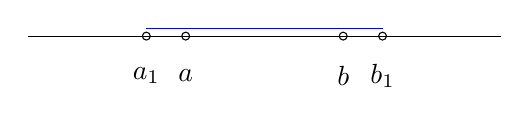
\begin{tikzpicture}
	\draw (-3,0) -- (3,0);
	\draw[blue] (-1.5,0.1) -- (1.5,0.1);
	\draw (-1,0) circle (0.05cm);
	\draw (-1,-0.5) node{$a$};
	\draw (1,0) circle (0.05cm);
	\draw (1,-0.5) node{$b$};

	\draw (-1.5,0) circle (0.05cm);
	\draw (-1.5,-0.5) node{$a_1$};
	\draw (1.5,0) circle (0.05cm);
	\draw (1.5,-0.5) node{$b_1$};
\end{tikzpicture}
\end{center}

		Suppose $b_1 < b$. Clearly, $a < b_1$. And the cover $\mathcal{C}$ must have an open interval containing $b_1$. Otherwise $\mathcal{C}$ is not a cover of $[a,b]$. That is, there exists $(a_2,b_2)$ containing $b_1 \in (a,b)$ such that $a_2 < b_1 < b_2$. If $b_2 > b$, then $\sum_{i=1}^k l(I_k) \ge l(a_1,b_1) + l(a_2,b_2) \ge l(a_1,b_2) \ge b-a$.

\begin{center}
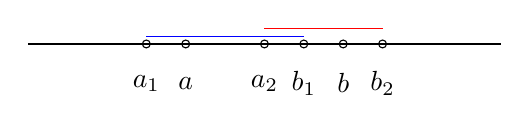
\begin{tikzpicture}
	\draw (-3,0) -- (3,0);
	\draw (-1,0) circle (0.05cm);
	\draw (-1,-0.5) node{$a$};
	\draw (1,0) circle (0.05cm);
	\draw (1,-0.5) node{$b$};

	\draw (-1.5,0) circle (0.05cm);
	\draw (-1.5,-0.5) node{$a_1$};
	\draw (0.5,0) circle (0.05cm);
	\draw (0.5,-0.5) node{$b_1$};
	\draw[blue] (-1.5,0.1) -- (0.5,0.1);

	\draw (0,0) circle (0.05cm);
	\draw (0,-0.5) node{$a_2$};
	\draw (1.5,0) circle (0.05cm);
	\draw (1.5,-0.5) node{$b_2$};
	\draw[red] (0,0.2) -- (1.5,0.2);
\end{tikzpicture}
\end{center}

		Suppose $b_2 < b$. Continuing like this we get, $N$ open intervals in $\mathcal{C}$, $\{ (a_k,b_k) : k = 1,2,\cdots,N \} $ such that $a_1 < a < b_1$ and $a_N < b < b_N$ and $a_k < b_{k-1} < b_k$ for all $k$. The process should terminate in fintie steps as $\mathcal{C}$ is a finite cover of $[a,b]$. Then $\sum_{k=1}^N l(I_k) \ge \sum_{k=1}^N l(a_k,b_k) \ge l(a_1,b_N) \ge b-a$.

\begin{center}
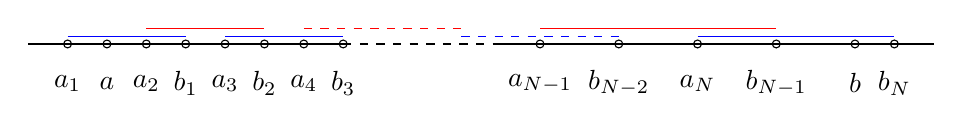
\begin{tikzpicture}
	\draw (-5,0) -- (-1,0);
	\draw[dashed] (-1,0) -- (1,0);
	\draw (1,0) -- (6.5,0);

	\draw (-4,0) circle (0.05cm);
	\draw (-4,-0.5) node{$a$};
	\draw (5.5,0) circle (0.05cm);
	\draw (5.5,-0.5) node{$b$};

	\draw (-4.5,0) circle (0.05cm);
	\draw (-4.5,-0.5) node{$a_1$};
	\draw (-3,0) circle (0.05cm);
	\draw (-3,-0.5) node{$b_1$};
	\draw[blue] (-4.5,0.1) -- (-3,0.1);

	\draw (-3.5,0) circle (0.05cm);
	\draw (-3.5,-0.5) node{$a_2$};
	\draw (-2,0) circle (0.05cm);
	\draw (-2,-0.5) node{$b_2$};
	\draw[red] (-3.5,0.2) -- (-2,0.2);

	\draw (-2.5,0) circle (0.05cm);
	\draw (-2.5,-0.5) node{$a_3$};
	\draw (-1,0) circle (0.05cm);
	\draw (-1,-0.5) node{$b_3$};
	\draw[blue] (-2.5,0.1) -- (-1,0.1);
	
	\draw (-1.5,0) circle (0.05cm);
	\draw (-1.5,-0.5) node{$a_4$};
	\draw[red,dashed] (-1.5,0.2) -- (0.5,0.2);

	\draw (2.5,0) circle (0.05cm);
	\draw (2.5,-0.5) node{$b_{N-2}$};
	\draw[blue,dashed] (0.5,0.1) -- (2.5,0.1);

	\draw (1.5,0) circle (0.05cm);
	\draw (1.5,-0.5) node{$a_{N-1}$};
	\draw (4.5,0) circle (0.05cm);
	\draw (4.5,-0.5) node{$b_{N-1}$};
	\draw[red] (1.5,0.2) -- (4.5,0.2);

	\draw (3.5,0) circle (0.05cm);
	\draw (3.5,-0.5) node{$a_N$};
	\draw (6,0) circle (0.05cm);
	\draw (6,-0.5) node{$b_N$};
	\draw[blue] (3.5,0.1) -- (6,0.1);
\end{tikzpicture}
\end{center}

	Clearly, every open cover of $[a,b]$ contains a finite subcover $\mathcal{C}$, which contains a finite subcover of the form $\{ (a_k,b_k) : k=1,2,\cdots,N \}$ such that $\sum_{k=1}^N l(I_k) \ge b-a$. Thus, for any open cover $\sum_{k=1}^\infty l(I_k) \ge b-a$. And thus,
	\begin{equation}
		m^\ast([a,b]) \ge b-a
	\end{equation}

	\textbf{Case 2 : Unbounded Interval}
	
	\end{proof}
	\item Outer Measure is translation invariant
	\item Outer Measure is countably subadditive
\end{enumerate}

\subsubsection{Outer Measure of Countable Sets}
\subsubsection{Outer Measure of Intervals}
\subsubsection{Outer Measure is translation invariant}
\subsubsection{Outer Measure is countably subadditive}

\subsection{Exercise}


\subsection{$\sigma$-algebra of Lebesgue Measurable Sets}




\part{}
\chapter{ME010301 Advanced Complex Analysis}
%Text Books : \cite{ahlfors}
%Module 1:
%Harmonic Functions - Definitions and Basic Properties, The Mean-Value Property, Poisson's Formula, Schwarz's Theorem, The Reflection Principle. A closer look at Harmonic Functions - Functions with Mean Value Property, Harnack's Principle.
%The Dirichlet's Problem - Subharmonic Functions, Solution of Dirichlet's Problem ( Proof of Dirichlet's Problem and Proofs of Lemma 1 and 2 excluded )
%(Chapter 4 : Section 6: 6.1 - 6.5, Chapter 6 : Section 3 : 3.1 - 3.2 , Section 4 : 4.1 - 4.2)
%Module 2:
%Power Series Expansions - Weierstrass's theorem, The Taylor Series, The Laurent Series Partial Fractions and Factorization - Partial Fractions, Infinite Products, Canonical Products, The Gamma Function. Entire Functions - Jensen's Formula, Hadamard's Theorem ( Hadamard's theorem - proof excluded)
%(Chapter 5 : Section 1 : 1.1 - 1.3, Section 2 : 2.1 - 2.4, Section 3 : 3.1 - 3.2 )
%Module 3:
%The Riemann Zeta Function - The Product Development, The Extension of $\zeta(s)$ to the Whole Plane, The Functional Equation, The Zeroes of the Zeta Function Normal Families - Normality and Compactness, Arzela's Theorem
%(Chapter 5 : Section 4 : 4.1 - 4.4, Section 5 : 5.2 - 5.3)
%Module 4:
%The Riemann Mapping Theorem - Statement and Proof, Boundary Behaviour, Use of the Reflection Principle
%The Weierstrass's Theory - The Weierstrass's $\rho$-function, The functions $\zeta(s)$ and $\sigma(z)$, The Differential Equation
%(Chapter 6 : Section 1: 1.1-1.3, Chapter 7 : Section 3 : 3.1 - 3.3)

\part{ME010301 Advanced Complex Analysis}
%Module 1 - \cite{ahlfors} 4
%Module 2 - \cite{ahlfors} 5
%Module 3 - \cite{ahlfors} 5
%Module 4 - \cite{ahlfors} 6, 7
%Missing - \cite{ahlfors} 8, 9, 10?

\chapter{ME010302 Partial Differential Equations}
%Text Books : \cite{sneddon}
%Module 1: (20 hours)
%Methods of solutions of $dx/P = dy/Q = dz/R$. Orthogonal trajectories of a system of curves on a surface. Pfaffian differential forms and equations. Solution of Pfaffian differential equations in three variables, Partial differential equations. Origins of first order partial differential equation.
%Module 2: (25 hours)
%Linear equations of first order. Integral surfaces passing through a given curve. Surfaces orthogonal to a given system of surfaces. Nonlinear partial differential equation of the first order . Compatible systems of first order equations . Charpits Method. Special types of first order equations. Solutions satisfying given conditions.
%Module 3: (20 hours)
%Jacobi's method The origin of second order equations. Linear partial differential equations with constant coefficients. Equations with variable coefficients.
%Module 4: (25 hours)
%Separation of variables. Non linear equations of the second order . Elementary solutions of Laplace equation. Families of equipotential surfaces. The two dimensional Laplace Equation Relation of the Logarithmic potential to the Theory of Functions.

%Module 1 - \cite{sneddon} 
%Module 2 - \cite{sneddon} 
%Module 3 - \cite{sneddon} 
%Module 4 - \cite{sneddon} 

\chapter{ME010303 Multivariate Calculus \& Integral Transforms}
%Text Books : \cite{apostol}, \cite{rudin}
%Module 1:
%The Weirstrass theorem, other forms of Fourier series, the Fourier integral theorem, the exponential form of the Fourier integral theorem, integral transforms and convolutions, the convolution theorem for Fourier transforms.
%(Chapter 11 Sections 11.15 to 11.21 of \cite{apostol}) (20 hours.)
%Module 2:
%Multivariable Differential Calculus, The directional derivative, directional derivatives and continuity, the total derivative, the total derivative expressed in terms of partial derivatives, An application of complex- valued functions, the matrix of a linear function, the Jacobian matrix, the matrix form of the chain rule. Implicit functions and extremum problems, the mean value theorem for differentiable functions,
%(Chapter 12 Sections. 12.1 to 12.11 of \cite{apostol}) (22 hours.)
%Module 3: 
%A sufficient condition for differentiability, a sufficient condition for equality of mixed partial derivatives, functions with non-zero Jacobian determinant, the inverse function theorem ,the implicit function theorem, extrema of real- valued functions of one variable, extrema of real-valued functions of several variables.
%Chapter 12 Sections-. 12.12 to 12.13 of \cite{apostol} 
%Chapter 13 Sections-. 13.1 to 13.6 of \cite{apostol} (28 hours.)
%Module 4:
%Integration of Differential Forms Integration, primitive mappings, partitions of unity, change of variables, differential forms.
%(Chapter 10 Sections. 10.1 to 10.14 of \cite{rudin}) (20 hours)

\part{ME010303 Multivariate Calculus \& Integral Transforms}
%Module 1 - \cite{apostol} 11
%Module 2 - \cite{apostol} 12
%Module 3 - \cite{apostol} 12, 13
%Module 4 - \cite{rudin} 10

\chapter{ME010304 Functional Analysis}
%Text Books : \cite{kreyszig}
%Module 1:
%Examples, Completeness proofs, Completion of Metric Spaces, Vector Space, Normed Space, Banach space, Further Properties of Normed Spaces, Finite Dimensional Normed spaces and Subspaces, Compactness and Finite Dimension
%(Chapter 1 - Sections 1.5, 1.6; Chapter 2 - Sections 2.1 to 2.5)
%Module 2:
%Linear Operators, Bounded and Continuous Linear Operators, Linear Functionals, Linear Operators and Functionals on Finite dimensional spaces, Normed spaces of operators, Dual space
%(Chapter 2 - Section 2.6 to 2.10)
%Module 3:
%Inner Product Space, Hilbert space, Further properties of Inner Product Space, Orthogonal Complements and Direct Sums, Orthonormal sets and sequences, Series related to Orthonormal sequences and sets, Total Orthonormal sets and sequences, Representation of Functionals on Hilbert Spaces
%(Chapter 3 - Sections 3.1 to 3.6, 3.8)
%Module 4:
%Hilbert-Adjoint Operator, Self-Adjoint, Unitary and Normal Operators, Zorn's lemma, Hahn- Banach theorem, Hahn-Banach theorem for Complex Vector Spaces and Normed Spaces, Adjoint Operators
%(Chapter 3 - Sections 3.9, 3.10; Chapter 4 - Sections 4.1 to 4.3, 4.5)

%Module 1 - \cite{kreyszig} 1
%Module 2 - \cite{kreyszig} 2
%Module 3 - \cite{kreyszig} 3
%Module 4 - \cite{kreyszig} 3, 4

%\chapter 1
\section{Metric Spaces}
The following are a few metric spaces and their distance functions,
\begin{enumerate}
	\item $\mathbb{R}, d(x,y) = |x -y|$
	\item $\mathbb{R}^2, d(x,y) = \left( |\xi_1-\eta_1|^2 + |\xi_2 - \eta_2|^2 \right)^\frac{1}{2} $ where $x = (\xi_1,\xi_2)$
	\item $\mathbb{R}^3, d(x,y) = \left( |\xi_1-\eta_1|^2 + |\xi_2 - \eta_2|^2 + |\xi_3-\eta_3|^2 \right)^\frac{1}{2} $ where $x = (\xi_1,\xi_2,\xi_3)$
	\item Euclidean space, $\displaystyle \mathbb{R}^n, d(x,y) = \left( \sum_{j=1}^n |\xi_j - \eta_j|^2 \right)^\frac{1}{2}$ where $x = (\xi_1,\xi_2,\dots,\xi_n)$
	\item $\mathbb{C}, d(x,y) = |x - y|$ where $x = a+ib$ and $|x| = (a^2+b^2)^\frac{1}{2}$
	\item Unitary space, $\displaystyle \mathbb{C}^n, d(x,y) =  \left( \sum_{j=1}^n |\xi_j - \eta_j|^2 \right)^\frac{1}{2}$ where  $x = (\xi_1,\xi_2)$ and $\xi_j \in \mathbb{C}$.
	\item $\displaystyle C[a,b], d(x,y) = \max_{t \in [a,b]} \left\{ |x(t)-y(t)| \right\}$ where $x$ is a continuous, complex-valued function defined on closed interval $[a,b] \subset \mathbb{R}$.
	\item $\displaystyle B(A), d(x,y) = \sup_{t \in A} \left\{ |x(t)-y(t)| \right\}$ where $x$ is a bounded, complex-valued function defined on $A \subset \mathbb{R}$
	\item $\displaystyle l^p, d(x,y) = \left( \sum_{j = 1}^\infty |\xi_j - \eta_j|^p \right)^\frac{1}{p}$ where $x = \sequence{\xi_j}$ and $\displaystyle \sum_{j=1}^\infty |\xi_j|^p < \infty$. That is, set of all sequences such that the $p$th power series is convergent.
	\item $\displaystyle l^\infty, d(x,y) = \sup_{j \in \mathbb{N}} \{ |\xi_j - \eta_j| \} $ where $x = \sequence{\xi_j}$ and $|\xi_j| \le c$. That is, $l^\infty$ is the space of all bounded sequences of complex numbers.
	\item $\displaystyle c, d(x,y) = \sup_{j \in \mathbb{N}} \{ |\xi_j - \eta_j| \}$ where $\sequence{\xi_j} = \xi_1,\xi_2,\dots$ is the space of all convergent sequences of complex numbers.
	\item $\displaystyle s, d(x,y) = \sum_{j = 1}^\infty \frac{1}{2^j} \frac{|\xi_j - \eta_j|}{1+|\xi_j-\eta_j|}$ where $x = \sequence{\xi_j} = \xi_1,\xi_2,\dots$ is the space of all sequence of complex numbers.
\end{enumerate}
Clearly, $l^p \subset l^\infty \subset s$.
But, $B(A),C[a,b]$ are non-comparable since there exists discontinuous, bounded functions and continuous, unbounded functions.

\begin{definition}[conjugate exponents]
	Real numbers $p,q$ are conjugates, if $p>1,q>1$ and $\frac{1}{p}+\frac{1}{q} = 1$.
\end{definition}
Note : if $p,q$ are conjugates, then $p+q=pq$ and $(p-1)(q-1) = 1$.
Also if $u = t^{p-1}$, then $t = u^{q-1}$.

\begin{theorem}[H\"older\footnote{O.H\"older} Inequality for sums]
	Let $p,q$ be conjugates and $(\xi_j), (\eta_j)$ be two complex sequences. $(\xi_j) \in l^p$ and $(\eta_j) \in l^q$.
	Then
	\begin{equation}
		\sum_{j=1}^\infty |\xi_j\eta_j| \le \left( \sum_{j=1}^\infty |\xi_j|^p \right)^\frac{1}{p} \quad \left( \sum_{j=1}^\infty |\eta_j|^q \right)^\frac{1}{q}
	\end{equation}
\end{theorem}
\begin{corollary}[Cauchy-Schwarz Inequality]
	When $p=2$, we have its conjugate $q=2$.
	Then H\"older inequality reduces to the following
	\begin{equation}
		\sum_{j=1}^\infty |\xi_j\eta_j| \le \left( \sum_{j=1}^\infty |\xi_j|^2 \right)^\frac{1}{2} \quad \left( \sum_{j=1}^\infty |\eta_j|^2 \right)^\frac{1}{2}
	\end{equation}

\end{corollary}
\begin{theorem}[Minkowski\footnote{H. Minkowski} Inequality]
	Let $p,q$ be conjugates and $(\xi_j), (\eta_j)$ be two complex sequences in $l^p$.
	Then
	\begin{equation}
		\left( \sum_{j=1}^\infty |\xi_j + \eta_j|^p \right)^\frac{1}{p} \le \left( \sum_{j=1}^\infty |\xi_j|^p \right)^\frac{1}{p} + \left( \sum_{j=1}^\infty |\eta_j|^q \right)^\frac{1}{q}
	\end{equation}
\end{theorem}
\subsection{A few more Concepts}
\begin{description}
	\item[product of metric spaces]
		Let $(X_1,d_1),(X_2,d_2)$ be two metric spaces.
		Let $x,y \in X_1 \times X_2$ where $x = (\xi_1,\xi_2 )$ and $y = (\eta_1,\eta_2)$.
		Then, $X_1 \times X_2$ is a metric space with following metrics,
		\begin{enumerate}
			\item $\displaystyle d(x,y) = d_1\left(\xi_1,\eta_1\right) + d_2\left(\xi_2,\eta_2\right)$
			\item $\displaystyle d(x,y) = \left( d_1\left( \xi_1,\eta_1 \right)^2 + d_2\left(\xi_2,\eta_2\right)^2 \right)^\frac{1}{2}$
			\item $\displaystyle d(x,y) = \max \{ d_1 \left(\xi_1,\eta_1\right) , d_2\left(\xi_2,\eta_2\right) \}$
		\end{enumerate}
	\item[separable] A space is separable if it has a countable, dense subset.\\
		Examples : $l^\infty$ is not separable. But, $l^p$ spaces are separable $(1 \le p <\infty)$. $\mathbb{R},\mathbb{C}$ are separable. $B[a,b]$ not seprable.
\end{description}
\subsection{Exercises}
\begin{enumerate}
	\item Find a sequence $\sequence{\xi_j}$ which converges to $0$ but does not belong to any $l^p$ space. $(1 \le p < \infty)$.
	\item Find a sequence $\sequence{\xi_j}$ which belong to $l^p$ space with $p>1$ but not in $l^1$.
\end{enumerate}
\setcounter{subsection}{4}
\subsection{Completeness}
Convergent sequences in a metric space are Cauchy sequences. But, Cauchy sequences are not necessarily convergent.
\begin{definition}[complete]
	A metric space is complete if every Cauchy sequence in it is convergent.
\end{definition}
\begin{theorem}
	$\mathbb{R}$ is complete.
\end{theorem}
\begin{proof}
	Let $\sequence{\xi_n}$ be a Cauchy sequence in $\mathbb{R}$.
	Let $M_0 > 0$.
	Then, there exists $N \in \mathbb{N}$ such that $\forall n,m > N,\ d(x_n,x_m) < M_0$.
	Let $M = \max \{M_0,M_1,\dots,M_N \}$ where $\forall n \le N,\ |\xi_j| < M_j$.
	Then $\sequence{\xi_n}$ is bounded by $M$.\\

	By Bolzano Weierstrass\dag\footnote{
		Every sequence has a monotone subsequence.
		And by monotone converges theorem, every monotone bounded sequence has a convergent subsequence.} 
	theorem, every bounded sequence in $\mathbb{R}^n$ has a convergent subsequence.
	Let $x \in \mathbb{R}$ be the limit of a convergent subsequence $\sequence{\xi_{n_k}}$ of $\sequence{\xi_n}$.
	Then $\xi_n \to x$ since $\sequence{\xi_n}$ is a Cauchy sequence.
\end{proof}

\begin{theorem}
	$\mathbb{C}$ is complete.
\end{theorem}
\begin{proof}
	Let $\sequence{\xi_n}$ be a Cauchy sequence in $\mathbb{C}$.
	Then the real, imaginary parts of $\xi_n$ are a Cauchy sequences in $\mathbb{R}$.
	We know that $\mathbb{R}$ is complete.
	Let $\Re(\xi_n) \to a$ and $\Im(\xi_n) \to b$.
	Then $\xi_n \to a+ib$ since $\sequence{\xi_n}$ is a Cauchy sequence.
\end{proof}

\begin{theorem}
	Finite dimensional Euclidean space, $\mathbb{R}^n$ is complete.
\end{theorem}
\begin{proof}
	Let $\sequence{x_k}$ be Cauchy sequence in $\mathbb{R}^n$.
	Let $\varepsilon > 0$.
	There exists $N \in \mathbb{N}$ such that $\forall m,r > N,\ d(x_m,x_r) < \varepsilon$.
	Let $x_m = (\xi_{1,m},\xi_{2,m},\dots,\xi_{n,m})$ and $x_r = (\xi_{1,r},\xi_{2,r},\dots,\xi_{n,r})$.
	\begin{align*}
		d(x_m,x_r) = \left( \sum_{j=1}^n |\xi_{j,m} - \xi_{j,r}|^2 \right)^\frac{1}{2} & <  \varepsilon\\
		\implies \sum_{j=1}^n |\xi_{j,m} - \xi_{j,r}|^2 & <  \varepsilon^2 \\
		\implies |\xi_{j,m} - \xi_{j,r}| & < \varepsilon^2,\ j = 1,2,\dots,n
	\end{align*}
	Therefore, $\sequence{\xi_{j,k}}$'s are Cauchy sequences in $\mathbb{R}$ for $j = 1,2,\dots,n$.
	Since $\mathbb{R}$ is convergent, $\xi_{j,k} \to \xi_j$ for each $j$.
	Let $x = (\xi_1,\xi_2,\dots,\xi_n)$.
	Let $\varepsilon > 0$.
	Then there exists $N_j \in \mathbb{N}$ such that $\forall m > N,\ |\xi_{j,m} - \xi_j|  < \frac{\varepsilon}{n} $.
	Let $N = \max \{ N_1,N_2,\dots,N_n\}$.
	Then $\forall m > N$,
	$$ d(x_m,x) = \left( \sum_{j=1}^n | \xi_{j,m} - \xi_j|^2 \right)^\frac{1}{2} = \left( \sum_{j=1}^n \frac{\varepsilon^2}{n^2} \right)^\frac{1}{2} = \frac{\varepsilon}{\sqrt{n}} < \varepsilon $$
	Therefore, $\sequence{x_n}$ converges to $x$ in $\mathbb{R}^n$.
\end{proof}

\begin{theorem}
	Finite dimensional Unitary space, $\mathbb{C}^n$ is complete.
\end{theorem}
\begin{proof}
	Same proof as above.
\end{proof}

\begin{theorem}
	The complex sequence space of all bounded sequences, $l^\infty$ is complete.
\end{theorem}
\begin{proof}
	Let $\sequence{x_k}$ be a Cauchy sequence in $l^\infty$ where $x_k = \xi_{k,1},\ \xi_{k,2},\ \dots$ are bounded sequences in $\mathbb{C}$ for each $k$.\\
	\textbf{Step 1 : Construct $x$}\\
	Let $\varepsilon > 0$.
	Then there exists $N \in \mathbb{N}$ such that $\forall m,n > N$,
	$$d(x_m,x_n) = \sup_{k \in \mathbb{N}} \left\{ \left|\xi_{m,k} - \xi_{n,k} \right| \right\} < \varepsilon $$
	From the metric, we have $\sequence{\xi_{j,k}}$'s are Cauchy sequences in $\mathbb{C}$ for each $k$.
	\begin{figure}
		$$\begin{matrix}
			x_1 = & \xi_{1,1} & \xi_{1,2} & \xi_{1,3} & \dots \\
			x_2 = & \xi_{2,1} & \xi_{2,2} & \xi_{2,3} & \dots \\
			x_3 = & \xi_{3,1} & \xi_{3,2} & \xi_{3,3} & \dots \\
			\vdots & \vdots & \vdots & \vdots & \vdots \\
			x = & \xi_1 & \xi_2 & \xi_3 & \dots 
		\end{matrix}$$
		\caption{Construction of limit in Sequence spaces}
	\end{figure}
	Thus, $\xi_{j,k} \to \xi_k \in \mathbb{C}$.
	Let $x = \xi_1,\ \xi_2,\ \dots $.
	Now we need to prove that $x_k \to x$ and $x \in l^\infty$.\\
	\textbf{Step 2 : $x \in l^\infty$}\\
	We have, $x_j \in l^\infty \implies |\xi_{m,j}| < c_j, \ \forall m \in \mathbb{N} $.
	Therefore,
	$$ |\xi_j| \le |\xi_j-\xi_{m,j}| + |\xi_{m,j}| \le \varepsilon + c_j, \quad \forall j \in \mathbb{N} $$
	Thus, $x \in l^\infty$.\\
	\textbf{Step 3 : $x_n \to x$}\\
	Since $|\xi_{m,j}-\xi_j| < \varepsilon$ for $m \in \mathbb{N}$,
	$$ d(x_m,x) = \sup_{j \in \mathbb{N}} |\xi_{m,j} - \xi_j| \le \varepsilon $$
\end{proof}

\begin{theorem}
	The complex sequence space of all convergent sequences, $c$ is complete
\end{theorem}
\begin{proof}
	Since every convergent sequence is bounded, $c \subset l^\infty$.
	And the sequence space $c$ is complete if $c$ is a closed subset of the complete space $l^\infty$.
	Therefore, it is sufficient to show that $c = \overline{c}$\\

	Let $x = \sequence{\xi_k} \in \overline{c}$.	
	Then there exists a convergent sequence $\sequence{x_k} = \sequence{\xi_{k,j}}$ in $c$ converging to $x$.
	That is, $\xi_{k,j} \to \xi_j$.\\

	Let $\varepsilon > 0$.
	Then there exists $N \in \mathbb{N}$ such that $\forall n \ge N$ and $\forall j,k \in \mathbb{N}$, we have $\displaystyle d(x_N,x) = \sup_{r \in \mathbb{N}} \{ |\xi_{n,r} - \xi_r| \} < \frac{\varepsilon}{3}$.
	Therefore,
	\begin{equation}
		|\xi_{N,j} - \xi_j| < \frac{\varepsilon}{3} \text{ and } |\xi_{N,k} - \xi_k| < \frac{\varepsilon}{3} 
	\end{equation}
	Every convergent sequence in complete metric space $l^\infty$ is also a Cauchy sequence.
	Since $x_N = \sequence{\xi_{N,k}}$ is a Cauchy sequence, there exists $N_1 \in \mathbb{N}$ and $\forall j,k \ge N_1$,
	\begin{equation}
		|\xi_{N,j} - \xi_{N,k}| < \frac{\varepsilon}{3}
	\end{equation}
	Therefore,
	$$|\xi_j - \xi_k| \le |\xi_j - \xi_{N,j}| + |\xi_{N,j}-\xi_{N,k}| + |\xi_{N,k} - \xi_k| \le \frac{\varepsilon}{3} + \frac{\varepsilon}{3} + \frac{\varepsilon}{3} = \varepsilon $$
	Clearly, $x = \sequence{\xi_k}$ is a Cauchy sequence in $l^\infty$.
	And since $l^\infty$ is complete, every Cauchy sequence in $l^\infty$ is convergent.
	Therefore, $x$ is a convergent sequence and $x \in c$.
	Thus, $c = \overline{c}$ and the induced\dag\footnote{
		Let $(X,d)$ be a complete metric space.
		And $Y$ is a closed subset of $X$.
		Then the induced metric space $(Y,d_{|_Y})$ is complete.}
	metric space $c$ is complete.
\end{proof}

\begin{theorem}
	For any $p \ge 1$, the sequence space $l^p$ is complete.
\end{theorem}
\begin{proof}
	Let $\sequence{x_k}$ be a Cauchy sequence $l^p$ where $x_k = \sequence{\xi_{k,j}}$ and
	$$ \sum_{j = 1}^\infty \left| \xi_{k,j} \right|^p < \infty,\ \forall k \in \mathbb{N} $$
	Since $\sequence{x_k}$ is a Cauchy sequence, for $\varepsilon > 0$ there exists $N \in \mathbb{N}$ such that
	\begin{equation}
		\label{equ:lpcauchy}
		d(x_m,x_n) = \left( \sum_{j=1}^\infty |\xi_{m,j} - \xi_{n,j}|^p \right) ^\frac{1}{p} < \varepsilon,\quad \forall m,n > N \text{ since } x_k \in l^p
	\end{equation}
	Thus, $\forall m,n > N,\ |\xi_{m,j} - \xi_{n,j}| < \varepsilon$ for each $j$.

	\textbf{Step 1 : Construction of $x$}\\
	Define $x = \sequence{\xi_j}$ where $\xi_j$ is an accumulation point of $\sequence{\xi_{k,j}}$.\\% Then $\xi_{k,j} \to \xi_j$ OR $x_k \to x$. \\

	\textbf{Step 2 : $x \in l^p$}\\
	Let $j > N$.
	Then, $\sequence{\xi_{k,j}}$ is a Cauchy sequence of complex numbers.
	Then, $\xi_{k,j} \to \xi_j$.
	Applying limit $n \to \infty$ on equation \ref{equ:lpcauchy}, we get
	\begin{align*}
		\left( \sum_{j=1}^\infty |\xi_{m,j} - \xi_j|^p \right) ^\frac{1}{p} & < \varepsilon,\quad \forall m > N \\
		\implies \sum_{j=1}^\infty |\xi_{m,j} - \xi_j|^p  & < \varepsilon^p
	\end{align*}
	Let $m > N$. Then $x_m - x \in l^p$. By Minkowski inequality, we have
	\begin{equation}
		\sum_{j=1}^\infty |\xi_j|^p  \le \sum_{j=1}^\infty |\xi_{m,j}-\xi_j|^p + \sum_{j=1}^\infty |\xi_{m,j}|^p  < \infty
	\end{equation}
	Thus, $x \in l^p$. \\
	\textbf{Step 3: $x_m \to x$}\\
	Since $\displaystyle \sum_{j=1}^\infty |\xi_{m,j} - \xi_j|^p < \varepsilon^p$, we have $\xi_{k,j} \to \xi_j$.
	Therefore, $x_m \to x$.
\end{proof}

\begin{theorem}
	The function space of all continuous functions defined on closed interval $[a,b]$, $C[a,b]$ is complete.
\end{theorem}
\begin{proof}
	Let $\sequence{x_k}$ be a Cauchy sequence in $C[a,b]$.\\
	Let $\varepsilon > 0$.
	Then there exists $N \in \mathbb{N}$ such that $m,n > N$, 
	$$ d(x_m,x_n) = \max_{t \in [a,b]} \left\{ x_m(t) - x_n(t) \right\} < \varepsilon $$
	Thus, for each $t \in [a,b]$, sequence $\sequence{x_k(t)}$'s are Cauchy sequences.
	We know that $\mathbb{C}$ is complete.
	Thus every Cauchy sequence in $\mathbb{C}$ is convergent.\\

	Define $x : [a,b] \to \mathbb{C}$ defined by $x(t) = $ the limit of the sequence $\sequence{x_k(t)}$.
	As $n \to \infty$, $d(x_m,x_n) \to d(x_m,x)$ and for any $m > N$, $d(x_m,x) < \varepsilon$ uniformly.
	It is evident from the construction that, the convergence $x_k(t) \to x(t)$ is uniform.\\

	Since the function $x_k$'s are continuous and the convergence is uniform, the limit function $x$ is also continuous.
	Therefore $x \in C[a,b]$.
\end{proof}

\begin{definition}[uniform metric]
	Let $(X,d)$ be a metric space in which every convergence $x_k \to x$ is uniform.
	Then the metric $d$ is a uniform metric.
\end{definition}
For example, the metric of $C[a,b]$ is a uniform metric.

\subsubsection{A few examples of incomplete metric spaces}
The following metric spaces are not complete,
\begin{enumerate}
	\item The space of rational numbers, $\mathbb{Q}$ with usual metric $d(x,y) = |x-y|$ is not complete since the rational approximations of $\pi$ is sequence in $\mathbb{Q}$ which doesn't converge in $\mathbb{Q}$.
		$$ 3,\ 3.1,\ 3.14,\ 3.141,\ \dots \to \pi \notin \mathbb{Q}$$
	\item The space of polynomial functions with metric $d(x,y) = \sup \{ x(t) - y(t)|$ is not complete since taylor approximations of $\sin x$ is a sequence of polynomial funcitons which doesn't converge to a polynomial function.
		$$ x,\ x+\frac{-x^3}{3!},\ x+\frac{-x^3}{3!}+\frac{x^5}{5!},\ \dots \to \sin x \notin p $$
	\item The space of continuous function on unit interval $[0,1]$ with a different\dag\footnote{Area under the graph of difference function is well-defined for integrable functions.} metric 
		$$ d(x,y) = \int_0^1 \left| x(t)-y(t) \right| \ dt $$
		is not complete since $\sequence{x_k}$ where $x_k : [0,1] \to \mathbb{R}$ is defined by
		$$x_k(t) = \begin{cases} 0 & t \in \left[0,\frac{1}{2}\right) \\
			(t-\frac{1}{2})k & t \in \left[\frac{1}{2},\frac{1}{2}+\frac{1}{k}\right) \\
		1 & t \in \left[\frac{1}{2}+\frac{1}{k},1\right] \end{cases} $$
		doesn't converge to a continuous polynomial function.
\end{enumerate}
\subsection{Completion of Metric Space}
Let $Y$ be an incomplete metric space.
Completion of $Y$ is a construction of a complete metric space $X$ in which $Y$ is dense.\\

For example, $\mathbb{Q}$ is not complete. However, $\mathbb{R}$ is a complete metric space in which $\mathbb{Q}$ is complete. Therefore, $\mathbb{R}$ is a completion of $\mathbb{Q}$.

\begin{definition}[Isometry]
	Isometric functions are distance preserving functions.
	And two metric spaces are isometric if there exists a bijective isometry between them.
\end{definition}

For example, function $f : X \to Y$ is an isometry if
$$ \forall x,y \in X,\quad \hat{d}(f(x),f(y)) = d(x,y)$$
where $d, \hat{d}$ are metrics in $X,Y$ respectively.
And if  $f$ is a bijection, then $X,Y$ are isometric space.\\

\begin{commentary}
	Two metric spaces are isometric is another way of saying that the spaces are identical (same) from metric point of view.
\end{commentary}

\begin{theorem}[completion]
	Let $(X,d)$ be a metric space.
	Then, there exists a complete metric space, $(\hat{X},\hat{d})$ such that it has a dense subspace $W$ which is isometric with $X$.
	And $\hat{X}$ is unique upto isomerties.
\end{theorem}
\begin{commentary}
	In other words, for any metric space $X$ there exists a unique complete metric space, $\hat{X}$ in which $X$ is dense.
\end{commentary}
\begin{proof}
	\textbf{Step 1 : Construction of $(\hat{X},\hat{d})$}\\
	Let $(X,d)$ be a metric space.
	Let $C$ be the set of all Cauchy sequence in $X$.
	Define relation $\sequence{x_k} \sim \sequence{y_k}$ if and only if $\displaystyle \lim_{k \to \infty} d(x_k,y_k) = 0$.
	This is an equivalence relation.(proof not required)

	\begin{commentary}
		{\footnotesize
		\begin{enumerate}
			\item Reflexive - $\displaystyle \hat{x} \sim \hat{x}$ since $\lim_{k \to \infty} d(x_k,x_k) = 0$. 
			\item Symmetric -  $\displaystyle \hat{x} \sim \hat{y} \implies \lim_{k \to \infty} d(x_k,y_k) = \lim_{k \to \infty} d(y_k,x_k) \implies \hat{y} \sim \hat{x}$.
		\item Transitive - Suppose, $\hat{x} \sim \hat{y}$ and $\hat{y} \sim \hat{z}$.\\
		$\displaystyle \hat{x} \sim \hat{y} \implies \hat{d}(\hat{x},\hat{y}) = \lim_{k \to \infty} d(x_k,y_k) = 0$, $\displaystyle \hat{y} \sim \hat{z} \implies \hat{d}(\hat{y},\hat{z}) = \lim_{k \to \infty} d(y_k,z_k) = 0$.\\
		Then $\displaystyle \hat{d}(\hat{x},\hat{z}) = \lim_{k \to \infty} d(x_n,z_n) \le \lim_{k \to \infty} d(x_n,y_n) + d(y_n,z_n) = \hat{d}(\hat{x},\hat{y}) + \hat{d}(\hat{y},\hat{z}) = 0$.\\
		Therefore $\hat{x} \sim \hat{z}$.
		\end{enumerate}
		}
	\end{commentary}

	Let $\hat{X}$ be the set of all equivalent classes in $C$.
	Define $\hat{d} : \hat{X} \times \hat{X} \to \mathbb{R}$ given by  $\displaystyle \hat{d}(\hat{x},\hat{y}) = \lim_{k \to \infty} d(x_k,y_k)$ where the Cauchy sequences $x_k \in \hat{x}$ and $y_k \in \hat{y}$.
	Then $\hat{d}$ is metric in $\hat{X}$.
	\begin{enumerate}
		\item $\hat{d}$ is well-defined\\
			Suppose $x_k,x_k' \in \hat{x}$ and $y_k,y_k' \in \hat{y}$.
			Then $x_k \sim x_k'$ and $y_k \sim y_k'$.
			In other words, $\displaystyle \lim_{k \to \infty} d(x_k,x_k') = 0$ and $\displaystyle \lim_{k \to \infty} d(y_k,y_k') = 0$.\\

			By triangular inequality, we have
			$$ d(x_k,y_k) \le d(x_k,x_k') + d(x_k',y_k') + d(y_k',y_k) $$
			$$ \implies d(x_k,y_k) - d(x_k',y_k') \le d(x_k,x_k') + d(y_k,y_k')$$
			Similarly,
			$$ d(x_k',y_k') - d(x_k,y_k) \le d(x_k,x_k') + d(y_k,y_k')$$
			Therefore, 
			$$ | d(x_k,y_k) - d(x_k',y_k')| \le d(x_k,x_k') + d(y_k,y_k')$$
			Apply the limit $k \to \infty$ on either sides, we get
			$$ \lim_{k\to \infty} |d(x_k,y_k)-d(x_k',y_k')| \le \lim_{k \to \infty} d(x_k,x_k') + \lim_{k \to \infty} d(y_k,y_k') = 0 $$
			Thus, $\hat{d}(x_k,y_k)$ depends only on the equivalent class $\hat{x},\hat{y}$ to which $x_k,y_k$ belongs and is independent of the representative from these equivalent classes.
			Therefore, $\hat{d} : \hat{X} \times \hat{X} \to \mathbb{R}$ is well-defined.
		\item $\hat{d}(\hat{x},\hat{y}) = 0 \iff \hat{x} = \hat{y}$
			$$ \hat{d}(\hat{x},\hat{y}) = 0 \iff \forall x_k \in \hat{x}, \forall y_k \in \hat{y},\ \lim_{k \to \infty} d(x_k,y_k) = 0 \iff x_k \sim y_k $$
		\item $\hat{d}(\hat{x},\hat{y}) = \hat{d}(\hat{y},\hat{x})$ is trivial since $d(x_k,y_k) = d(y_k,x_k)$.
		\item $\hat{d}(\hat{x},\hat{y}) \le \hat{d}(\hat{x},\hat{z}) + \hat{d}(\hat{z},\hat{y})$
			$$ d(x_k,y_k) \le d(x_k,z_k) + d(z_k,y_k) $$
			Applying limit $k \to \infty$ on either sides, we get
			$$ \hat{d}(\hat{x},\hat{y}) = \lim_{k \to \infty} d(x_k,y_k) \le \lim_{k \to \infty} d(x_k,z_k) + \lim_{k \to \infty} d(z_k,y_k)  = \hat{d}(\hat{x},\hat{z}) + \hat{d}(\hat{z},\hat{y})$$
	\end{enumerate}
	\textbf{Step 2: Construction of Isometry $T : X \to W,\ W \subset \hat{X}$.}\\
	---yet to update---
	\textbf{Step 3: $\hat{X}$ is complete}\\
	\textbf{Step 4: Uniqueness of $\hat{X}$}\\
\end{proof}
%\chapter 2
\section{Banach Spaces}
%\chapter 3
\section{Hilbert Spaces}
%\chapter 4
\section{Fundamental Theorems for Banach Spaces}

\chapter{ME010305 Optimization Technique}
%Text Books : \cite{mital}, \cite{solberg}
%Module 1 : Linear Programming
%Simplex Method, Canonical form of equations, Simplex Method (Numerical Example), Simplex Tableau, Finding the first BFS and artificial variables, Degeneracy, Simplex multipliers, Revised simplex method, Duality in LPP, Duality theorems, Applications of Duality, Dual simplex method, Summery of simplex methods.
%(Chapter 3; sections: 9 - 21 of \cite{mital}) (25 hours)
%Module 2 : Integer Programming
% I. L. P. in two dimensional space, General I.L.P. and M.I.L.P. problems, cutting planes, remarks on cutting plane methods, branch and bound method, examples, general description, the 0-1 variable.
%(Chapter 6; sections: 6.1 - 6.10 of \cite{mital}) (25 hours)
%Module 3 : Goal Programming, Flow and potentials in Networks
%Goal programming. Graphs- definitions and notation, minimum path problem, spanning tree of minimum length, problem of minimum potential difference, scheduling of sequential activities, maximum flow problem, duality in the maximum flow problem, generalized problem of maximum flow.
%(Chapter - 5 & 7 Sections 5.9 & 7.1 to 7.9, 7.15 of \cite{mital}) (15 hours)
%Module 4 : Non-linear Programming
%Basic concepts - Taylor’s series expansion, Fibonacci Search, golden section search, Hooke and Jeeves search algorithm, gradient projection search, Lagrange multipliers, equality constraint optimization, constrained derivatives, non-linear optimization: Kuhn-Tucker conditions, complimentary Pivot algorithms.
%(Chapter 11; Sections: 11.1 - 11.7, 11.9- 11.11 of \cite{solberg}) (25 hours)

%Module 1 - \cite{mital} 3
%Module 2 - \cite{mital} 6
%Module 3 - \cite{mital} 5, 7
%Module 4 - \cite{solberg} 11

%Module 1
\section{Linear Programming}
\begin{definition}[LPP]
Linear Programming Problem (LPP) is the optimization of linear object function under certain linear equality/inequalities constraints.
\end{definition}
\paragraph{General LPP}
A general LPP is of the form,
\begin{align}
	\text{ minimise } & : & f(X) = CX  & \text{ (object function)} \label{eqn:obj} \\
	\text{ subject to } & : & AX = B & \text{ (linear constraints)}\label{eqn:sub} \\
	\text{ such that } & & X \ge 0 & \text{ (non-negativity conditions)}\label{eqn:positive}
\end{align}

	That is,
\begin{align}
\text{ minimise } & : & f = c_1x_1 + c_2x_2 + \dotsb + c_nx_n & \\
\text{ subject to } & : & \begin{pmatrix} a_{11} & a_{12} & \dots & a_{1m} \\ a_{21} & a_{22} & \dots & a_{2m} \\ \vdots & \vdots & \ddots & \vdots \\ a_{m1} & a_{m2} & \dots & a_{mm} \end{pmatrix} \begin{pmatrix} x_1 \\ x_2 \\ \dots \\ x_m \end{pmatrix} & = \begin{pmatrix} b_1 \\ b_2 \\ \vdots \\ b_m \end{pmatrix} \\
\text{ such that } & & X \ge 0 &
\end{align}

	The coefficients of the object function, $c_i$ are the \textbf{cost coefficients}.

\paragraph{Feasible Solution} is a vector $X$ satisfying both constraints and non-negativity constraints. The set of all feasible solutions is denoted by $S_F$. This is a convex set and is often represented graphically by a polytope.

\paragraph{Basic Solution} In an LPP with $m$ constraints and $n$ variables, a \textbf{basic solution} is a vector $X$ in which $n-m$ variables are zero. These variables are the non-basic variables and the remaining $m$ variables are the basic variable. The set of all basic variables is a \textbf{basis}.

\paragraph{Basic Feasible Solution} is a basic solution which is feasible. The \textbf{b.f.s.} are vertices of the polytope $S_F$ (if nonempty).

\paragraph{Optimal Solution} is a vector $X$ which optimizes the object function $f$. For a bounded $S_F$, always there exists a b.f.s which is optimal.

\paragraph{Solving LPP} Due to the presence of inequalities, there is no analytic tool for solving an LPP. There are a few numerical methods for solving an LPP. Simplex is popular among them.

\paragraph{Simplex Algorithm}
	First, we compute a b.f.s. (which is a vertex of the polytope $S_F$). If there is a desirable b.f.s. (an  adjancent vertex) which improves the object function, then we jump to the corresponding b.f.s. (vertex). We continue this process until there is no scope of further improvement.

\paragraph{Canonical Form}
	Consider the LPP (in matrix form)
\begin{align*}
\text{ minimise } & f(X) = CX \\
\text{ subject to } & AX = B \\
\text{ such that } & X \ge 0  
\end{align*}
\begin{commentary}
\begin{align*}
	\intertext{Rearranging the non-basic variable, we get}
	\begin{pmatrix} a_{11} & a_{12} & \dots & a_{1m} \\ a_{21} & a_{22} & \dots & a_{2m} \\ \vdots & \vdots & \ddots & \vdots \\ a_{m1} & a_{m2} & \dots & a_{mm} \end{pmatrix} \begin{pmatrix} x_1 \\ x_2 \\ \vdots \\ x_m \end{pmatrix} & = \begin{pmatrix} b_1 - a_{1,(m+1)} x_{m+1} - a_{1,(m+2)} x_{m+2} - \dotsb - a_{1n}x_n \\ b_2 - a_{2,(m+1)} x_{m+1} - a_{2,(m+2)} x_{m+2} - \dotsb - a_{2,n}x_n \\ \vdots \\ b_m-a_{m,(m+1)}x_{m+1} - a_{m,(m+2)}x_{m+2}-\dotsb-a_{m,n}x_n \end{pmatrix}
\end{align*}
Left multplying with $A^{-1}$ on either sides, we get
\begin{align*}
	\begin{pmatrix} x_1 \\ x_2 \\ \vdots \\ x_m \end{pmatrix} = & \begin{pmatrix} \bar{b}_1 - \bar{a}_{1,(m+1)} x_{m+1} - \bar{a}_{1,(m+2)} x_{m+2} - \dotsb - \bar{a}_{1n}x_n \\ \bar{b}_2 - \bar{a}_{2,(m+1)} x_{m+1} - \bar{a}_{2,(m+2)} x_{m+2} - \dotsb - \bar{a}_{2,n}x_n \\ \vdots \\ \bar{b}_m-\bar{a}_{m,(m+1)}x_{m+1} - \bar{a}_{m,(m+2)}x_{m+2}-\dotsb-\bar{a}_{m,n}x_n \end{pmatrix}\\
		\text{where } & \begin{pmatrix} \\ A^{-1} \\ \hphantom{} \end{pmatrix} \begin{pmatrix} b_1 \\ b_2 \\ \dots \\ b_m \end{pmatrix} = \begin{pmatrix} \bar{b}_1 \\ \bar{b}_2 \\ \vdots \\ \bar{b}_m \end{pmatrix} \text{ and } \begin{pmatrix} \\ A^{-1} \\ \hphantom{} \end{pmatrix} \begin{pmatrix} a_{1,(m+1)} \\ a_{2,(m+1)} \\ \vdots \\ a_{m,(m+1)} \end{pmatrix} = \begin{pmatrix} \bar{a}_{1,(m+1)} \\ \bar{a}_{2,(m+1)} \\ \vdots \\ \bar{a}_{m,(m+1)} \end{pmatrix}
\end{align*}

The constraints \[ \sum_{j=1}^n a_{ij}x_j = b_i, \qquad j = 1,2,\dots,n \] in the form, \[ x_i + \sum_{j=m+1}^n \bar{a}_{i,j} = \bar{b}_i, \qquad i=1,2,\dots,m\] is said to be canonical.
Also we can replace $x_i$'s in object function to get, 
\[ f(X) = \sum_{i=1}^m c_i \left( \bar{b}_i - \sum_{j=m+1}^n \bar{a}_{ij}x_j \right) + \sum_{j=m+1}^n c_jx_j = \sum_{i=1}^m c_i\bar{b}_i + \sum_{i=m+1}^n \bar{c}_jx_j \]
where $\displaystyle \bar{c}_j = c_j - \sum_{i=1}^m c_i \bar{a}_{ij},\ j = m+1,m_2,\dots,n$.
 From the canonical form, we can compute the corresponding b.f.s., $X = (\bar{b}_1,\bar{b}_2,\dots,\bar{b}_m,0,0,\dots,0)$ and object function $\displaystyle f(X) = \sum_{i=1}^m \bar{b}_ic_i $ since $\bar{c}_j$ are zero for $j > m$. These $\bar{c}_j$'s are called the \textbf{relative cost coefficients}.
\end{commentary}

\subsection{Simplex Method}
\begin{align*}
\text{ minimise : } & f(x) = 6x_1 - 2x_2 +4x_3 - 5x_4\\
\text{ subject to : } & 4x_1 - x_2 + 2x_3 - 3x_4 \le 1 \\
& x_2 + 4x_3 - 2x_4 \le 2 \\
& x_1,x_2,x_3,x_4 \ge 0
\end{align*}
\begin{figure}[hbt]
\centering
\begin{tabular}{c|c|c|c|c|c|c|c|c|}\hline
Phase & Basis & B & $P_1$ & $P_2$ & $P_3$ & $P_4$ & $P_5$ & $P_6$ \\ \hline
1 & $x_5$ & 1 & 4 & -1 & 2 & \textcolor{red}{$3$} & 1 & 0  \\ 
  & $x_6$ & 2 & 0 &  1 & 0 & $4$ & 0 & 1 \\ \hline
  & $f$   & 0 & 6 & -2 & 4 & -5 & 0 & 0 \\ \hline
	2 & $x_4$ & $\sfrac{1}{3}$ & $\sfrac{4}{3}$ & $\sfrac{-1}{3}$ & $\sfrac{2}{3}$ & 1 & $\sfrac{1}{3}$ & 0  \\ 
	& $x_6$ & $\sfrac{2}{3}$ & $\sfrac{-16}{3}$ & \textcolor{red}{$\sfrac{7}{3}$} & $\sfrac{-8}{3}$ & 0 & $\sfrac{-4}{3}$ & 1 \\ \hline
	& $f$ & $\sfrac{5}{3}$ & $\sfrac{38}{3}$ & $\sfrac{-11}{3}$ & $\sfrac{22}{3}$ & 0 & $\sfrac{5}{3}$ & 0 \\ \hline
	3 & $x_4$ & $\sfrac{3}{7}$ & $\sfrac{4}{7}$ & 0 & $\frac{2}{7}$ & 1 & \textcolor{red}{$\sfrac{1}{7}$} & $\sfrac{1}{7}$  \\ 
	& $x_2$ & $\sfrac{2}{7}$ & $\sfrac{-16}{7}$ & 1 & $\sfrac{-8}{7}$ & 0 & $\sfrac{-4}{7}$ & $\sfrac{3}{7}$ \\ \hline
	& $f$ & $\sfrac{19}{7}$ & $\sfrac{30}{7}$ & 0 & $\sfrac{22}{7}$ & 0 & $\sfrac{-3}{7}$ & $\sfrac{11}{7}$ \\ \hline
	4 & $x_5$ & 3 & 4 & 0 & 2 & 7 & 1 & 1 \\
	  & $x_2$ & 2 & 0 & 1 & 0 & 4 & 0 & 1 \\ \hline
	  & $f$   & 4 & 6 & 0 & 4 & 3 & 0 & 2 \\ \hline
\end{tabular}
\caption{Simplex Steps}
\end{figure}

\subsection{Unrestricted Variable}
\begin{align*}
\text{ minimise : } & f(x) = 6x_1 - 2x_2 +4x_3 - 5x_4\\
\text{ subject to : } & 4x_1 - x_2 + 2x_3 - 3x_4 \le 1 \\
& x_2 + 4x_3 - 2x_4 \le 2 \\
& x_1,x_2,x_4 \ge 0 \text{ and } x_3 \text{ unrestricted}
\end{align*}
	In above LPP, the variable $x_3$ is unrestricted. Replace $x_3$ with two variables $x_{31}$ and $x_{32}$ such that $x_3 = x_{31}-x_{32},\ x_{31} \ge 0,\ x_{32} \ge 0$. We get,
\begin{align*}
	\text{ minimise : } & f(x) = 6x_1 - 2x_2 +4x_{31}-4x_{32} - 5x_4\\
	\text{ subject to : } & 4x_1 - x_2 + 2x_{31}-2x_{32} - 3x_4 \le 1 \\
	& x_2 + 4x_{31}-4x_{32} - 2x_4 \le 2 \\
	& x_1,x_2,x_{31},x_{32},x_4 \ge 0
\end{align*}

\subsection{Artificial Variable}
\begin{align*}
\text{ minimise : } & f(x) = 6x_1 - 2x_2 +4x_3 - 5x_4\\
\text{ subject to : } & 4x_1 - x_2 + 2x_3 - 3x_4 \le 1 \\
& x_2 - 4x_3 + 2x_4 \le -2 \\
& x_1 - 2x_2 + x_3 \le -5 \\
& x_1,x_2,x_3,x_4 \ge 0
\end{align*}
First, we need to change all right-hand side constants into on-negative.
\begin{align*}
\text{ minimise : } & f(x) = 6x_1 - 2x_2 +4x_3 - 5x_4\\
\text{ subject to : } & 4x_1 - x_2 + 2x_3 - 3x_4 \le 1 \\
& -x_2 + 4x_3 - 2x_4 \ge 2 \\
& -x_1 + 2x_2 - x_3 \ge 5 \\
& x_1,x_2,x_3,x_4 \ge 0
\end{align*}
Now we need to introduce three slack variables $x_5,x_6,x_7$,
\begin{align*}
\text{ minimise : } & f(x) = 6x_1 - 2x_2 +4x_3 - 5x_4\\
\text{ subject to : } & 4x_1 - x_2 + 2x_3 - 3x_4 + x_5 = 1 \\
& -x_2 + 4x_3 - 2x_4 - x_6 = 2 \\
& -x_1 + 2x_2 - x_3 - x_7 = 5 \\
& x_1,x_2,x_3,x_4,x_5,x_6,x_7 \ge  0
\end{align*}

\subsubsection{Two Phase Method}
First phase we compute a basic feasible solution (b.f.s.) for the first iteration the simplex method from an auxiliary problem with the artificial variables $x_8,x_9$ each introduced into '$\ge$' constraints. In second phase, original problem is optimized using simplex method.\\

	If the auxiliary problem does not have a feasible solution in which every artificial variables are zero, then original LPP has no feasible solution.\\

Phase I: Auxiliary Problem
\begin{align*}
	\text{ minimise : } & g(x) = x_8 + x_9 \\
\text{ subject to : } & 4x_1 - x_2 + 2x_3 - 3x_4 + x_5 = 1 \\
& -x_2 + 4x_3 - 2x_4 - x_6 + x_8 = 2 \\
& -x_1 + 2x_2 - x_3 - x_7 + x_9 = 5 \\
& x_1,x_2,x_3,x_4,x_5,x_6,x_7,x_8,x_9 \ge  0
\end{align*}

Phase II: Origial Problem with an initial b.f.s. 
---to be corrected---
\begin{align*}
	\text{ minimise : } & f(x) = 6x_1 - 2x_2 +4x_3 - 5x_4 \\
\text{ subject to : } & 4x_1 - x_2 + 2x_3 - 3x_4 + x_5 = 1 \\
& -x_2 + 4x_3 - 2x_4 - x_6 + x_8 = 2 \\
& -x_1 + 2x_2 - x_3 - x_7 + x_9 = 5 \\
& x_1,x_2,x_3,x_4,x_5,x_6,x_7,x_8,x_9 \ge  0
\end{align*}

\subsubsection{Big M Method}
In Big M method, arbitrarily large multiples of artificial variables are added to the object function. If the optimal solution of the modified problem has any artificial variables with nonzero value, then it has no feasible solution.
\begin{align*}
	\text{ minimise : } & f(x) = 6x_1 - 2x_2 +4x_3 - 5x_4 + 100x_8 + 100x_9 \\
\text{ subject to : } & 4x_1 - x_2 + 2x_3 - 3x_4 + x_5 = 1 \\
& -x_2 + 4x_3 - 2x_4 - x_6 + x_8 = 2 \\
& -x_1 + 2x_2 - x_3 - x_7 + x_9 = 5 \\
& x_1,x_2,x_3,x_4,x_5,x_6,x_7,x_8,x_9 \ge  0
\end{align*}

%Module 2
\section{Integer Programming}
\begin{definition}
	Integer Linear Programming Problem(ILPP) is the integral conditioning of an optimization of a linear object function under certain linear equality/inequality constraints.
\end{definition}

\paragraph{General ILPP}
A general ILPP is of the form,
\begin{align}
	\text{ minimise } & : & f(X) = & CX  \text{ (object function)} \label{eqn:obj} \\
	\text{ subject to } & : & AX = & B \text{ (constraints)}\label{eqn:sub} \\
	\text{ such that } & & X \ge & 0 \text{ (non-negativity conditions)}\label{eqn:positive} \\
	and & & X \text{ is an integer vector}. & \text{ (integer condition) }
\end{align}

\begin{remark}
	Let $T_F$ be the set of all integer solutions.
	Let $[T_F]$ be the convex hull of $T_F$.
	Let $S_F$ be the set of all real solutions.
	Then, $T_F \subset [T_F] \subset S_F$.\\
	
	Finding optimal solution from $T_F$ is a much more difficult than finding optimal solution from $[T_F]$. Using Simplex method on $[T_F]$, we can find the optimal integer solutions.
\end{remark}
\pagebreak

%Module 3
\section{Networks}
\subsection{Introduction}
	Networks finds its applications in electrical circuits, transportation/logistics, communication systems.

\subsection{Graphs : Definition, Notation}
\begin{commentary}
	You don't have to learn the exact definition. But should know the differences. Definition of $\Omega^+, \Omega^-$ are important.
\end{commentary}

\begin{description}
	\item[Graph] $G(V,U)$ or $G$ is a set $V$ of elements $v_1,v_2,\dots,v_n$ represented by points and a set $U$ of pairs $(v_j,v_k),\ v_j,v_k \in V$ represented by arcs joining points of $V$.
	\item[Vertices] are the elements of $V$ in graph $G(V,U)$.
	\item[Arcs] are the elements of $U$ in graph $G(V,U)$.
	\item[Directed Arcs] An arc is directed if the pair $(v_j,v_k)$ is an ordered pair. Directed arcs are represented by arcs with a direction. 
	\item[Directed Graph] is the graph with directed arcs.
	\item[Subgraph] $G_1(V_1,U_1)$ of a graph $G(U,V)$ is a graph $G_1(V_1,U_1)$ such that $V_1 \subset V$ and $U_1$ contains \textcolor{red}{all arcs} of $G$ between the vertices of $G$.
	\item[Partial Graph] $G_1(V_1,U_1)$ of a graph $G(U,V)$ is a graph $G_1(V_1,U_1)$ such that $V_1 \subset V$ and $U_1 \subset U$.
	\item[$\Omega^+(v_k)$] is the set of all vertices incident to $v_k$.
	\item[$\Omega^-(v_k)$] is the set of all vertices incident from $v_k$.
	\item[Chain] is a sequence of arcs $u_1,u_2,\dots,u_q$ in which every intermediate arc $u_k$ has one vertex common with both previous $u_{k-1}$ and next $u_{k+1}$ vertices.
	\item[Cycle] is a chain in which no arc is used twice and first and last vertices have a common vertex.
	\item[Path] is a chain in which all arcs are directed in the same sense such that terminal vertex of preceeding arc is the initial vertex of the succeeding arc.
	\item[Circuit] is a cycle in which all arcs are directed in the same sense. 
	\item[Connected] A graph is connected if every pair of vertices have a chain connecting them. 
	\item[Component] is the set a vertex $v_a$ of all other vertices connetced to $v_a$ by chains.
	\item[Strongly Connected] A graph is strongly connected if there is a path connecting every pair of vertices in it.
	\item[Tree] is a connected graph with at least two verties and no cycles.
	\item[Centre] is a vertex which is connected to every other vertex of the graph by a path.
	\item[Arborescence] is a tree with a centre.
\end{description}

\subsection{Minimum Path Problem}
\begin{definition}[Minimum Path Problem]
	Let $x_{jk}$ be the real numbers associated to each arc $(v_j,v_k$. Let $v_a, v_b$ be two vertices of $G$. The length of a path from $v_a$ to $v_b$ is $\sum x_{jk}$ where the summation is over sequence of all arcs forming the path. The minimum path problem is to find the path of the smallest length among various path from $v_a$ to $v_b$.
\end{definition}

\begin{remark}
In general, $x_{jk}$ is unrestricted in sign.
\end{remark}

\subsubsection{All arc lengths are nonnegative}
\begin{commentary}
	The problem solved using an algorithm which is similar to proof by mathematical induction. 
	Initial step is trivial $V_0 = \{ v_a \}$. Hypothesis is that problem is solved for every vertex in $V_p$ for $p = k$. Our task is to find $V_{k+1}$ using $V_k$. The process is repeated till $v_b \in V_p$.
\end{commentary}

	Let $f_j$ be the length of the minimum path from $v_a$ to $v_j$. Then $f_a = 0$. And our goal is to find $f_b$.

\begin{commentary}
	Here, $p$ represents the stage. $V_p$ is the set of all vertices for which $f_j$ is known for every $v_j \in V_p$.
\end{commentary}

	$V_p$ is the set of all vertices for which minimum path problem is solved. The problem is solved when $v_b \in V_p$ for some $p$.

\begin{commentary}
	In each step, we find the vertex $v_s \notin V_p$ such that out of all the arcs leaving $V_p$, a particular arc incident on $v_s$ forms the minimum length path.
\end{commentary}

	$\Omega^-(V_p)$ is the set of all arcs going out a vertex in $V_p$ and let 
$$ f_r + x_{rs} = \min_{\Omega^-(V_p)} f_j + x_{jk} $$

\begin{commentary}
	This means that, we have found vertices $v_r \in V_p$, $v_s \notin V_p$ such that the arc $(v_r,v_s)$ forms the minimum length path leaving out of $V_p$ when it is combined with minimum length path to $v_r$ which is already known.
\end{commentary}

	Then, we repeat the process with $V_p = V_p \cup \{ v_s \}$ as $f_s = f_r + x_{rs}$ is the length of minimum path from $v_a$ to $v_s$.

	We start with $p = 0$, $V_0 = \{v_a\}$ and $f_a = 0$. Repeating the process we will get a sequence of sets $V_1,V_2,\dots$ if there is a set $V_k$ containing $v_b$ then minimum path length $f_b$ is found. If there is not such set in that sequence, then there is no path from $v_a$ to $v_b$.

\begin{example}
	Question : Find minimum path from $v_0$ to $v_8$ in the graph shown in figure \ref{dia:minPath1}. The number along the a directed arc denotes its length.

\begin{figure}
\centering
\begin{tikzpicture}
	\tikzset{arc/.style={postaction={decorate}, decoration={markings,mark=at position #1  with {\arrow{latex}}, }}}
	\begin{scope}
	\tikzstyle every node=[draw,circle]
	\draw (0,0) node(v0){$0$};
	\draw (2,2) node(v1){$1$};
	\draw (2,0) node(v2){$2$};
	\draw (2,-2) node(v3){$3$};
	\draw (6,2) node(v4){$4$};
	\draw (4,0) node(v5){$5$};
	\draw (6,-2) node(v6){$6$};
	\draw (8,1) node(v7){$7$};
	\draw (10,-1) node(v8){$8$};
	\end{scope}
	\draw[arc=0.5] (v0)--(v1) node (l1)[midway,label=above:$2$]{};
	\draw[arc=0.5] (v0)--(v2) node (l2)[midway,label=above:$6$]{};
	\draw[arc=0.5] (v0)--(v3) node (l3)[midway,label=above:$8$]{};
	\draw[arc=0.5] (v1)--(v4) node (l4)[midway,label=above:$10$]{};
	\draw[arc=0.5] (v1)--(v5) node (l5)[midway,label=above:$8$]{};
	\draw[arc=0.5] (v2)--(v5) node (l6)[midway,label=above:$1$]{};
	\draw[arc=0.5] (v3)--(v5) node (l7)[midway,label=above:$2$]{};
	\draw[arc=0.5] (v3)--(v6) node (l8)[midway,label=above:$4$]{};
	\draw[arc=0.5] (v4.30) to[out=20,in=100] (v7.90);
	\path (v4)--(v7) node(l9)[midway,label=above:$3$]{};
	\draw[arc=0.5] (v7.150) to[out=180,in=300] (v4.330);
	\path (v7)--(v4) node(l10)[midway,label=right:$2$]{};
	\draw[arc=0.5] (v5)--(v4) node (l11)[midway,label=above:$1$]{};
	\draw[arc=0.5] (v5)--(v7) node (l12)[midway,label=above:$5$]{};
	\draw[arc=0.5] (v6)--(v5) node (l13)[midway,label=above:$4$]{};
	\draw[arc=0.5] (v6.90) to[out=100,in=200] (v7.210);
	\path (v6)--(v7) node(l14)[midway,label=left:$6$]{};
	\draw[arc=0.5] (v7.270) to[out=280,in=20] (v6.30);
	\path (v7)--(v6) node(l15)[midway,label=right:$1$]{};
	\draw[arc=0.5] (v6)--(v8) node (l16)[midway,label=above:$7$]{};
	\draw[arc=0.5] (v7)--(v8) node (l17)[midway,label=above:$10$]{};
\end{tikzpicture}
\caption{Minimum Path Problem : Non-negative Arc Length}
\label{dia:minPath1}
\end{figure}

\begin{center}
\begin{tabular}{*{8}{c}}
	$p$ & $V_p$ & $f$ & $\Omega^-(V_p)$ & $x$ & $f+x$ & $f_s$ & $v_s$ \\ \hline
	0 & 0 & 0 & (0,1) & 2 & 2 & 2 & 1 \\
	& & & (0,2) & 6 & 6 & & \\
	& & & (0,3) & 8 & 8 & & \\ \hline
\end{tabular}
\end{center}

\begin{commentary}
	In Step 0, $p = 0$ and $V_p = \{ v_0 \}$. In column $V_p$, we wrote $0$ instead of $v_0$. And we know that, $f_0 = 0$. The arc incidents out of $v_0$ are $(0,1), (0,2), (0,3)$. These arcs are listed in column $\Omega^-(V_p)$. The arc length of $(0,1)$ is $x_{01} = 2$ which is wrote under the column $x$. In the first row, $f_j + x_{jk} = f_0 + x_{01}$, the sum is wrote under the column $f+x$.

	After completing all these columns, the least sum in column $f+x$ is seleted and wrote in the same row in column $f_s$ and the respective vertex is available in $\Omega^-(V_p)$ column in the same row as the second vertex of the arc. Here, it is $(0,1)$ and thus $v_s = 1$. Now Step 0 is complete and $V_p = \{ 0,1 \}$ as $v_s$ added to $V_p$. But, problem is not solved as $v_8 \notin V_p$. Thus we proceed to Step 1.
\end{commentary}

\begin{center}
\begin{tabular}{*{8}{c}}
	$p$ & $V_p$ & $f$ & $\Omega^-(V_p)$ & $x$ & $f+x$ & $f_s$ & $v_s$ \\ \hline
	1 & 0 & 0 & (0,2) & 6 & 6 & & \\
	& & & (0,3) & 8 & 8 & & \\
	& 1 & 2 & (1,2) & 3 & 5 & 5 & 2 \\
	& & & (1,4) & 10 & 12 & & \\
	& & & (1,5) & 8 & 10 & & \\ \hline
\end{tabular}
\end{center}

\begin{commentary}
	In Step 1, $p = 1$ and $V_p = \{v_0,v_1\}$. Each row of the table corresponds to each arc going out of $V_p$. There are two arcs incident from $v_0$ and three arcs incident from $v_1$.Thus there are two row for $v_0$ and three rows for $v_1$. Note that the arc $(0,1)$ is not considered as it has both end vertices in $V_p$.
	
	Then length of the arcs are wrote. It is added to the value in column $f$ and wrote in column $f+x$. The minimum value in column $f+x$ is selected. It corresponds to the arc $(1,2)$. Thus the vertex is $v_2$ and the length of minimum path from $v_0$ to $v_2$ is $5$.
\end{commentary}

Repeating the process a few more times, you will find that the minimum length path from $v_0$ to $v_8$ is $0,1,2,6,8$ and its length is $17$.(do it yourself)
\end{example}

\subsubsection{Arc lengths unrestricted in sign}
\pagebreak

%Module 4
\section{Non-linear Programming}



\part{}
\chapter{ME010401 Spectral Theory}
%Text Books : \cite{kreyszig}
%Module 1:
%Reflexive Spaces, Category theorem(statement only), Uniform Boundedness theorem ( applications excluded), Strong and Weak Convergence, Convergence of Sequences of Operators and Functionals, Open Mapping Theorem, Closed Linear Operators, Closed Graph Theorem
%(Chapter 4 - Sections 4.6 to 4.9, 4.12, 4.13) (20 Hours)
%Module 2:
%Banach Fixed point theorem, Spectral theory in Finite Dimensional Normed Spaces, Basic Concepts, Spectral Properties of Bounded Linear Operators, Further Properties of Resolvent and Spectrum, Use of Complex Analysis in Spectral Theory
%(Chapter5 – Section 5.1; Chapter 7 - Sections 7.1 to 7.5) (25 Hours)
%Module 3:
%Banach Algebras, Further Properties of Banach Algebras, Compact Linear Operators on Normed spaces, Further Properties of Compact Linear Operators, Spectral Properties of compact Linear Operators on Normed spaces, Further Spectral Properties of Compact Linear Operators 
%(Chapter 7 - Sections 7.6, 7.7; Chapter 8 - Sections 8.1 to 8.4) ( 25 Hours)
%Module 4:
%Spectral Properties of Bounded Self adjoint linear operators, Further Spectral Properties of Bounded Self Adjoint Linear Operators, Positive Operators, Projection Operators, Further Properties of Projections
%(Chapter 9 - Sections 9.1 to 9.3, 9.5, 9.6) (20 Hours)

%Module 1 - \cite{kreyszig} 4.6,7,8,9,12,13
%\chapter 1
\setcounter{section}{3}
{\Large Module 1}
\section{Normed and Banach Spaces}
\setcounter{subsection}{5}
\subsection{Reflexive Spaces}
\begin{commentary}
\begin{description}
	\item[Algebraically Reflexive]
		A vector space $X$ is algebraically reflexive if the canoical mapping $C : X \to X^{\ast\ast}$ defined by $C(x) = g_x \in X^{\ast\ast}$ is surjective where $X^\ast, X^{\ast\ast}$ are the first and second algebraic dual spaces of $X$ and $\forall f \in X^\ast,\ g_x(f) = f(x)$.\cite[\S2.8]{Kreyszig}\\

	\item Finite dimensional vector spaces are algebraically reflexive.\cite[\S2.9.3]{Kreyszig}
\end{description}
\end{commentary}

\begin{commentary}
\paragraph{Summary}
\begin{enumerate}
	\item Reflexive $\implies$ Completeness
	\item Completeness $\nimplies$ Reflexive
	\item Finite Dimensional $\implies$ Reflexive
	\item Hilbert Space $\implies$ Reflexive
	\item Separable space with non-separable dual space is non-reflexive
	\item $X^\prime$ separable $\implies X$ separable
\end{enumerate}
\end{commentary}

\begin{lemma}
	For every fixed $x \in X$, the funcitonal $g_x : X^\prime \to X$ defined by $g_x(f) = f(x)$ is a bounded linear functional on $X'$ so that $g_x \in X^{\prime\prime}$, and has the norm
	\[ \|g_x\| = \|x\| \]
\end{lemma}
\begin{proof}
	From Hahn-Banach theorem for normed spaces, we know that for any $x \in X$
	\begin{equation}
		\|x\|  = \sup_{\substack{f \in X'\\ f \ne 0}} \frac{|f(x)|}{\|f\|}  =  \sup_{\substack{f \in X' \\ f \ne 0}} \frac{|g_x(f)|}{\|f\|} = \|g_x\| 
	\end{equation}
	Clearly, $g_x$ is bounded, $g_x \in X^{\prime\prime}$ and $\|g_x\| = \|x\|$.
\end{proof}

\begin{lemma}
	The Canonical mapping $C : X \to X^{\prime\prime}$ given by $C(x) = g_x$ such that $\forall f \in X^\prime,\ g_x(f) = f(x)$ is an isomorphism of $X$ onto $\mathscr{R}(C)$.
\end{lemma}
\begin{proof}
	\textbf{Step 1 : $C$ is linear}
	\begin{equation}
	g_{\alpha x + \beta y} = f(\alpha x + \beta y) = \alpha f(x) + \beta f(y) = \alpha g_x(f) + \beta g_y(f)
	\end{equation}
	\indent Therefore, $C$ is linear.\\

	\textbf{Step 2 : $C$ is injective}\\
	\indent We have, $C$ is linear.
	Thus, $g_{x-y} = g_x - g_y$.
	Then,
	\begin{equation}	
		\| C(x) - C(y) \| = \| g_x - g_y \| = \|g_{x-y}\| = \|x-y\|
	\end{equation}
	\indent Thus, $C$ is an isometry.
	Therefore, $C$ is injective.\\

	Therefore, $C$ is an isomorphism from $X$ onto $\mathscr{R}(C)$.
\end{proof}

\begin{definition}[Reflexive]
	A normed space $X$ is reflexive if the canonical mapping $C : X \to X^{\prime\prime}$ defined by $C(x) = g_x$ such that $\forall f \in X^\prime,\ g_x(f) = f(x)$ is surjective where $X^\prime, X^{\prime\prime}$ are the first and second dual spaces of $X$.
\end{definition}

Example, $\mathbb{R}^n$ is reflexive since ${\mathbb{R}^n}^{\prime\prime} = {\mathbb{R}^n}^\prime = \mathbb{R}^n$.

\begin{theorem}
	Reflexive $\implies$ Completeness
\end{theorem}
\begin{proof}
	Let $X$ be a reflexive normed space.
	Then $C : X \to X^{\prime\prime}$ is surjective and $X \simeq X^{\prime\prime}$.
	We know that, $X^{\prime\prime}$ is a dual space of $X^\prime$.
	Thus, $X^{\prime\prime}$ is complete since $B(X^\prime,K)$ is a Banach space.
	Therefore, $X$ is complete.
\end{proof}

\begin{theorem}
	Finite dimensional $\implies$ reflexive
\end{theorem}
\begin{proof}
	Let $X$ be a finite dimensional normed space.
	Then every linear operator $T : X \to K$ is bounded.
	Thus, $X^\prime = X^\ast$ and $dim\ X = dim\ X^\ast$.
	Thus, $X^{\prime\prime} = X^{\ast\ast}$.
	We know that, finite dimensional normed spaces are algebraically reflexive.
	Thus, $\mathscr{R}(C) = X^{\ast\ast} = X^{\prime\prime}$.
	Therefore, $X$ is reflexive.
\end{proof}
\subsection{Category Theory}
\subsection{Strong and Weak Convergence}
\subsection{Convergence of Sequences of Operators and Functionals}
%\subsection{Application to Summability of Sequences}
%\subsection{Numerical Integration and Weak\ast Convergence}
\setcounter{subsection}{11}
\subsection{Open Mapping Theorem}
\subsection{Closed Linear Operators}
\pagebreak

%Module 2 - \cite{kreyszig} 5.1, 7.1,2,3,4,5
{\Large Module 2}
\section{Linear Operators}
\subsection{Bananch Fixed Point Theorem}
%\subsection{Application of Bananch Theorem to Linear Equations}
\setcounter{section}{6}
\section{Spectral Theory of Linear Operators in Normed Spaces}
\subsection{Spectral Theory in Finite Dimensional Normed Spaces}
\subsection{Basic Concepts}
\subsection{Spectral Properties of Bounded Linear Operators}
\subsection{Further Properties of Resolvant and Spectrum}
\subsection{Use of Complex Analysis in Spectral Theory}
\pagebreak

%Module 3 - \cite{kreyszig} 7.6,7, 8.1,2,3,4
{\Large Module 3}
\subsection{Banach Algebra}
\subsection{Further Properties of Banach Algebra}

\section{Compact Linear Operators}
\subsection{Compact Linear Operators on Normed Spaces}
\subsection{Further Properties of Compact Linear Operators}
\subsection{Spectral Properties of Compact Linear Operators on Normed Spaces}
\subsection{Further Spectral Properties of Compact Linear Operators}
\pagebreak

%Module 4 - \cite{kreyszig} 9.1,2,3,5,6
{\Large Module 4}
\section{Bounded, Self-Adjoint Linear Operators}
\subsection{Spectral Properties of Bounded Self-Adjoint Linear Operators}
\subsection{Further Spectral Properties of Bounded Self-Adjoint Linear Operators}
\subsection{Positive Operators}
%\subsection{Square Roots of a Positive Operator}
\setcounter{subsection}{4}
\subsection{Projection Operators}
\subsection{Further Properties of Projections}
%Missing - Chapter 6, 10

\chapter{ME010402 Analytic Number Theory}
%Text Books : \cite{apostol2}
%Module 1:
%Arithmetic Functions, Dirichlet Multiplication and Averages of Arithmetical functions Arithmetic Functions, Dirichlet Multiplication : Introduction, The M\"{o}bius function $\mu(n)$, The Euler totient function $\phi(n)$, a relation connecting $\mu$ and $\phi$, a product formula for $\phi(n)$, The Dirichlet product of arithmetical functions, Dirichlet inverses and the M\"{o}bius inversion formula, The Mangoldt function $\wedge(n)$, Multiplicative functions, Multiplicative functions and Dirichlet Multiplication, The inverse of a completely multiplicative function, The Liouville's function $\lambda(n)$, The divisor function $\sigma_\alpha(n)$, Generalized convolutions.
%Averages of Arithmetical functions : Introduction, The big-oh notation, Asymptotic equality of functions, Eulers summation formula, Some elementary asymptotic formulas, The average order of $d(n)$,The average order of the divisor functions $\sigma_\alpha(n)$, The average order of $\phi(n)$, An application to the distribution of lattice points visible from the origin, The average order of $\mu(n)$ and of $\wedge(n)$, The partial sums of a Dirichlet product, Applications to $\mu(n)$ and of $\wedge(n)$.
%(Chapter 2: sections 2.1 to 2.14, Chapter 3:3.1 to 3.11)  (30 hours)
%Module 2:
%Some Elementary Theorems on the Distribution of Prime Numbers Introduction, Chebyshev's functions $\psi(x)$ and $\theta(x)$, Relation connecting $\theta(x)$ and $\pi(x)$, Some equivalent forms of the prime number theorem, Inequalities for $\pi(n)$ and $P_n$, Shapiro's tauberian theorem, Applications of Shapiro's theorem, An asymptotic formula for the partial sum $\sum_{p \le x} 1/p$.
%(Chapter 4: sections 4.1 to 4.8) (15 hours)
%Module 3:
%Congruences:  Definitions and basic properties of congruences, Residue classes and complete residue system, Linear congruences, Reduced residue systems and Euler-Fermat theorem, Polynomial congruences modulo p, Lagrange's theorem, Applications of Lagrange's theorem, Simultaneous linear congruences, The Chinese remainder theorem, Applications of the Chinese remainder theorem.
%(chapter 5: 5.1 to 5.8) (25 hours)
%Module 4:
%Quadratic Residues, The Quadratic Reciprocity Law and Primitive Roots, Quadratic Residues, The Quadratic Reciprocity Law : Quadratic residues, Legendre's symbol and its properties, evaluation of $(-1/p)$ and $(2/p)$, Gauss' Lemma, The quadratic reciprocity law, Applications of the reciprocity law.
%Primitive Roots : The exponent of a number $\mod m$, Primitive roots, Primitive roots and reduced residue systems, The nonexistence of primitive roots $\mod 2^\alpha$ for $\alpha \ge 3$, The existence of primitive root $\mod p$ for odd primes $p$, Primitive roots and quadratic residues.
%(Chapter 9; 9.1 to 9.6)
%(Chapter 10: 10.1 to 10.5) (20 hours)

\part{ME010402 Analytic Number Theory}
%Module 1 - \cite{apostol2} 2
%Module 2 - \cite{apostol2} 4
%Module 3 - \cite{apostol2} 5
%Module 4 - \cite{apostol2} 9, 10


\chapter{ME800401 Differential Geometry}
%ME800401
%Module 1:
%Graphs and level sets, vector fields, the tangent space, surfaces, vector fields on surfaces, orientation.
%(Chapters 1 to 5 of \cite{thorpe}) (20 hours)
%Module 2:
%The Gauss map, geodesics, Parallel transport,
%(Chapters 6, 7 & 8 of \cite{thorpe}) (20 hours)
%Module 3:
%The Weingarten map, curvature of plane curves, Arc length and line integrals
%(Chapters 9, 10 & 11 of \cite{thorpe}) (25 hours)
%Module 4:
%Curvature of surfaces and Parametrized surfaces
%(Chapters 12 & 14 of \cite{thorpe}) (25 hours)

%Module 1 - \cite{thorpe} 1, 2, 3, 4, 5
%Module 2 - \cite{thorpe} 6, 7, 8
%Module 3 - \cite{thorpe} 9, 10, 11
%Module 4 - \cite{thorpe} 12, 14
%Missing - 13, 15, 16?

%\chapter{Graphs and Level Sets}
\section{Graphs and Level Set}
\begin{definition}
	Let function $f : U \to \mathbb{R}$ where $U \subset \mathbb{R}^{n+1}$.
	Let $c$ be a real number.
	Then the \textbf{Level set} of $f$ at height $c$ is the set of all points in $U$ with image $c$.
	\begin{equation}
		f^{-1}(c) = \{ (x_1,x_2,\cdots,x_{n+1}) \in U : f(x_1,x_2,\cdots,x_{n+1}) = c \}
	\end{equation} 
\end{definition}

\begin{definition}
	Let function $f : U \to \mathbb{R}$ where $U \subset \mathbb{R}^{n+1}$.
	Then,
\begin{equation}
	graph(f) = \{ (x_1,x_2,\cdots,x_{n+2}) \in \mathbb{R}^{n+2} : f(x_1,x_2,\cdots,x_{n+1}) = x_{n+2} \}
\end{equation}
\end{definition}

\begin{figure}[h]
	\centering
	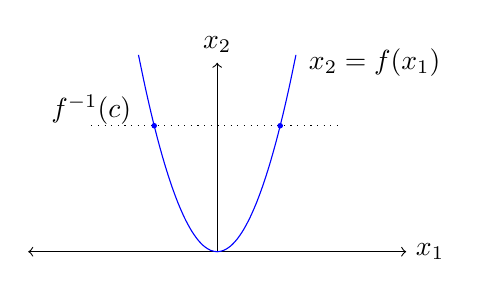
\begin{tikzpicture}[scale=0.8]
		\draw[<->] (-3, 0) -- (3, 0) node[right] {$x_1$};
  		\draw[->] (0, 0) -- (0, 3) node[above] {$x_2$};
  		\draw[scale=0.5, domain=-2.5:2.5, smooth, variable=\x, blue] plot ({\x}, {\x*\x});
		\draw[dotted,thin,black] (-2,2) -- (2,2);
		\draw (-2,2.25) node{$f^{-1}(c)$};
		\draw (2.5,3) node{$x_2 = f(x_1)$};
		\node[circle,fill=blue,inner sep=0pt, minimum size=2pt] at (1,2){};
		\node[circle,fill=blue,inner sep=0pt, minimum size=2pt] at (-1,2){};
\end{tikzpicture}
	\caption{Graph of $f(x_1)=x_1^2$ and Level set $f^{-1}(c)$}
\end{figure}

%\chapter{Vector Fields}
\section{Vector Fields}
\begin{definition}
	A vector $\mathbf{v}$ at a point $p \in \mathbb{R}^{n+1}$ is a pair $\mathbf{v} = (p,v)$ where $v \in \mathbb{R}^{n+1}$.
\end{definition}
\begin{description}
	\item[vector addition] $\mathbf{v} + \mathbf{w} = (p,v) + (p,w) = (p,v+w)$.
	\item[scalar multiplication] Let $c \in \mathbb{R}$, then $c \mathbf{v} =  c(p,v) = (p,cv)$.
	\item[dot product] $\mathbf{v}\cdot \mathbf{w} = (p,v)\cdot(p,w) = v \cdot w$
	\item[cross product] $\mathbf{v}\times \mathbf{w} = (p,v)\times(p,w) = (p,v \times w)$
\end{description}
\begin{remark}
	Angle $\theta$ between $\mathbf{v}$ and $\mathbf{w}$ is given by,
	\begin{equation}
		\cos \theta = \mathbf{v}\cdot\mathbf{w} = (p,v)\cdot(p,w) = v.w
	\end{equation}
	And the length of a vector $\mathbf{v}$ is given by,
	\begin{equation}
		\|\mathbf{v}\| = \mathbf{v}\cdot\mathbf{v} = (p,v)\cdot(p,v) = v\cdot v = \| v \|
	\end{equation}
\end{remark}

\begin{remark}
	Let $c \in \mathbb{R}$ and $p \in \mathbb{R}^{n+1}$. Let $\mathbf{v}, \mathbf{w}$ be two vectors at $p$. That is, $\mathbf{v} = (p,v)$ and $\mathbf{w} = (p,w)$ for some $v,w \in \mathbb{R}^{n+1}$. Then the set of all vectors at $p$ is a vector space with vector addition $\mathbf{v}+\mathbf{w} = (p,v+w)$ and scalar multiplication $c\mathbf{v} = (p,cv)$. This vector space is denoted by $\mathbb{R}_p^{n+1}$.
\end{remark}

\begin{figure}[h]
	\centering
	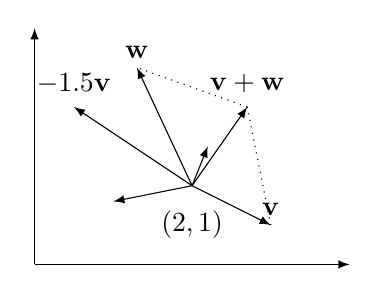
\begin{tikzpicture}
		\draw[-latex] (0,0) -- (0,3);
		\draw[-latex] (0,0) -- (4,0);

		\draw[-latex] (2,1) -- (1,0.8);
		\draw[-latex] (2,1) -- (2.2,1.5);
		%\draw[-latex] (2,1) -- (3,1.25);
		\draw[-latex] (2,1) -- (1.3,2.5); %w
		\draw[-latex] (2,1) -- (3,0.5); %v
		\draw[-latex] (2,1) -- (2.7,2); %v+w
		\draw[-latex] (2,1) -- (0.5,2); %1.5v
		\draw[dotted,thin] (3,0.5) -- (2.7,2);
		\draw[dotted,thin] (2.7,2)-- (1.3,2.5);

		\draw (2,0.5) node{$(2,1)$};
		\draw (3,0.7) node{$\mathbf{v}$};
		\draw (1.3,2.7) node{$\mathbf{w}$};
		\draw (2.7,2.3) node{$\mathbf{v+w}$};
		\draw (0.5,2.3) node{$-1.5\mathbf{v}$};
	\end{tikzpicture}
	\caption{The vector space of all vectors at $(2,1)$, $\mathbb{R}_{(2,1)}^2$}
\end{figure}

\begin{definition}
	The vector field $\mathbf{X}$ on $\mathbb{R}^{n+1}$ is a function which assigns to each point of $\mathbb{R}^{n+1}$ a vector at that point.
	That is, $\mathbf{X}(p) = (p,X(p))$.
\end{definition}

For example, $\mathbf{X}(p) = (p,X(p))$ where the associated function of the vector field, $X : \mathbb{R}^2 \to \mathbb{R}^2$ defined by $X(p) = (1,2)$ assigns a constant vector $(1,2)$ at every vector in $\mathbb{R}^2$.

\begin{figure}[h]
	\centering
	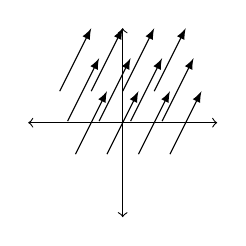
\begin{tikzpicture}[scale=0.4]
		\draw[<->] (-3,0) -- (3,0);
		\draw[<->] (0,-3) -- (0,3);

		\draw[-latex] (1,1) -- (2,3);
		\draw[-latex] (0,1) -- (1,3);
		\draw[-latex] (-1,1) -- (0,3);
		\draw[-latex] (-2,1) -- (-1,3);

		\draw[-latex] (1.25,0.05) -- (2.25,2.05);
		\draw[-latex] (0.25,0.05) -- (1.25,2.05);
		\draw[-latex] (-0.75,0.05) -- (0.25,2.05);
		\draw[-latex] (-1.75,0.05) -- (-0.75,2.05);

		\draw[-latex] (1.5,-1) -- (2.5,1);
		\draw[-latex] (0.5,-1) -- (1.5,1);
		\draw[-latex] (-0.5,-1) -- (0.5,1);
		\draw[-latex] (-1.5,-1) -- (-0.5,1);

	\end{tikzpicture}
	\caption{Vector field with associated function $X(p) = (1,2)$}
\end{figure}

\begin{definition}[smooth]
	A function $f : \mathbb{R} \to \mathbb{R}$ is smooth if its partial derivatives of all orders exists and are continuous.
	A function $f : \mathbb{R}^{n+1} \to \mathbb{R}$ is smooth if its component functions $f = (f_1, f_2, \cdots, f_{n+1})$ are smooth.
	A vector field $\mathbf{X}$ is smooth if the associated function $X(p)$ is smooth.
\end{definition}

\begin{definition}
	Let $f : \mathbb{R}^{n+1} \to \mathbb{R}$. Then the gradient of $f$ at $p$ is,
	\begin{equation}
		\nabla f(p) = \left(p,\frac{\partial f}{\partial x_1}(p),\frac{\partial f}{\partial x_2}(p),\cdots,\frac{\partial f}{\partial x_{n+1}}(p)\right)
	\end{equation}
\end{definition}

\begin{remark}
	If $f$ is a smooth function, then the gradient of $f$ at $p$ is a smooth vector field.
\end{remark}
	For example, $f : \mathbb{R}^2 \to \mathbb{R}$ defined by $f(x_1,x_2) = 2x_1x_2$ is a smooth function. We have, $\frac{\partial f}{\partial x_1} = 2x_2$ and $\frac{\partial f}{\partial x_2} = 2x_1$. And gradient of $f$ at $(x_1,x_2)$ is $(x_1,x_2,2x_2,2x_1)$. That is, $(2x_2,2x_1)$ at $(x_1,x_2)$.

Calculations : \\
\begin{tabular}{|c|c|c|c|c|c|c|} \hline
	$p$    & $(x_1,x_2)$   & $(0,0)$ & $(1,0)$ & $(0,1)$ & $(-1,0)$ & $(0,-1)$ \\ \hline
	$X(p)$ & $(2x_2,2x_1)$ & $(0,0)$ & $(0,2)$ & $(2,0)$ & $(0,-2)$ & $(-2,0)$ \\ \hline
\end{tabular}

\begin{figure}[h]
	\centering
	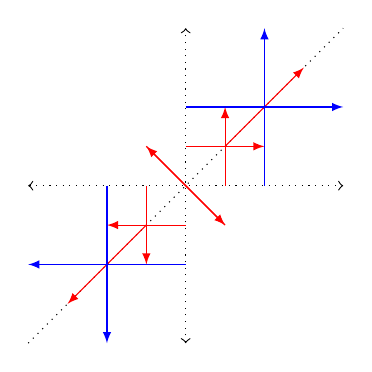
\begin{tikzpicture}[scale=0.5]
		\draw[<->,dotted] (0,-4) -- (0,4);
		\draw[<->,dotted] (-4,0) -- (4,0);
		\draw[dotted] (-4,-4) -- (4,4);

		\draw[-latex,color=red] (1,1) -- (3,3);
		\draw[-latex,color=red] (-1,1) -- (1,-1);
		\draw[-latex,color=red] (1,-1) -- (-1,1);
		\draw[-latex,color=red] (-1,-1) -- (-3,-3);
		\draw[-latex,color=red] (0,1) -- (2,1);
		\draw[-latex,color=red] (0,-1) -- (-2,-1);
		\draw[-latex,color=red] (1,0) -- (1,2);
		\draw[-latex,color=red] (-1,0) -- (-1,-2);

		%\draw[-latex] (-1,2) -- (3,0);
		%\draw[-latex] (2,-1) -- (0,3);
		%\draw[-latex] (1,-2) -- (-3,0);
		%\draw[-latex] (-2,1) -- (0,-3);

		\draw[-latex,color=blue] (0,2) -- (4,2);
		\draw[-latex,color=blue] (2,0) -- (2,4);
		\draw[-latex,color=blue] (-2,0) -- (-2,-4);
		\draw[-latex,color=blue] (0,-2) -- (-4,-2);

		%\draw[-latex] (1,0.5) -- (2,2.5);
		%\draw[-latex] (0.5,1) -- (2.5,2);
		%\draw[-latex] (-1,0.5) -- (0,-1.5);
		%\draw[-latex] (0.5,-1) -- (-1.5,0);
		%\draw[-latex] (1,-0.5) -- (0,1.5);
		%\draw[-latex] (-0.5,1) -- (1.5,0);
		%\draw[-latex] (-1,-0.5) -- (-2,-2.5);
		%\draw[-latex] (-0.5,-1) -- (-2.5,-2);
	\end{tikzpicture}
	\caption{The gradient of $f(x_1,x_2) = 2x_1x_2$}
\end{figure}

\begin{definition}
	A parameterised curve is a function, $\alpha : I \to \mathbb{R}^{n+1}$ where $I$ is some open interval in $\mathbb{R}$.
	The velocity vector of a parameterised curve $\alpha : I \to \mathbb{R}^{n+1}$ at a point $\alpha(t)$ is the tangent to the curve at that point.
	\begin{equation}
		\dot{\mathbf{\alpha}}(t) = \left(\alpha(t),\frac{d \alpha}{dt} (t)\right)
	\end{equation}
\end{definition}

For example, $\alpha : I \to \mathbb{R}^2$ defined by $\alpha(t) = (2t,t^2)$ is a parameterised curve. We have, $\frac{d\alpha}{dt} = (\frac{dx_1}{dt}(t),\frac{dx_2}{dt}(t)) = (2,2t)$ where $\alpha(t) = (x_1(t),x_2(t))$. The velocity vector at $t = 3$ is $\dot{\alpha}(3) = (\alpha(t),\frac{d\alpha}{dt}) = (6,9,2,6)$.

\begin{definition}
	Let $\mathbf{X}$ be a vector field and let $U$ be an open subet of $\mathbb{R}^{n+1}$.
	An integral curve $\alpha$ on $U$ is a parameterised curve, $\alpha : I \to \mathbb{R}^{n+1}$ such that for each $\alpha(t) = p \in U$, the velocity vector $\dot{\alpha}(t)$ is the associated vector $\mathbf{X}(p)$ of the vector field $\mathbf{X}$ at that point. Thus, for each $t \in I$, $\dot{\alpha}(t) = \mathbf{X}(\alpha(t))$.
	\begin{equation}
		\left(\alpha(t),\frac{d \alpha}{dt}(t)\right) = \left(\alpha(t),X(\alpha(t))\right)
	\end{equation}
	Let $X(p) = \left(X_1(p),X_2(p),\cdots,X_{n+1}(p)\right)$ and $\alpha(t) = \left(x_1(t),x_2(t),\cdots,x_{n+1}(t)\right)$. Then, comparing components of the vector at $\alpha(t)$ we get the following system of equations,
	\begin{equation}
		\frac{d x_j}{dt}(t) = X_j(\alpha(t)),\ j = 1,2,\cdots,(n+1)
	\end{equation}
\end{definition}

For example, Consider $\alpha : (2,3) \to \mathbb{R}^2$ defined by $\alpha(t) = (t,t^2)$. Then $\alpha$ is a parameterised curve in vector field, $\mathbf{X}$ which has the associated function $X(x_1,x_2) = (1,2x_1)$. Then, $\mathbf{X}(x_1,x_2) = (x_1,x_2,1,2x_1)$. And
\[ \dot{\alpha}(t) = \left( \alpha(t),\frac{d\alpha}{dt}(t) \right) = \left( x_1(t),x_2(t),\frac{dx_1}{dt}(t), \frac{dx_2}{dt}(t) \right) = (t,t^2,1,2t) \]
Clearly, $\alpha$ is an integral curve of $\mathbf{X}$ as $\dot{\alpha}(t) = X(\alpha(t))$ for every $t \in (2,3)$.

Calculations:\\
\begin{tabular}{|c|c|c|c|c|c|c|c|c|c|} \hline
	$p$    & $(0,0)$ & $(1,0)$ & $(0,1)$ & $(1,1)$ & $(-1,0)$ & $(0,-1)$ & $(-1,1)$ & $(1,-1)$ & $(-1,-1)$ \\ \hline
	$X(p)$ & $(1,0)$ & $(2,2)$ & $(1,1)$ & $(2,3)$ & $(0,-2)$ & $(1, 1)$ & $(0,-1)$ & $(2, 1)$ & $( 0,-3)$ \\ \hline
\end{tabular}

\begin{figure}[h]
	\centering
	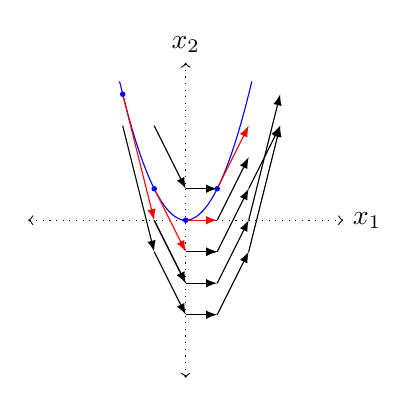
\begin{tikzpicture}[scale=0.4]
		\draw[<->,dotted] (-5, 0) -- (5, 0) node[right] {$x_1$};
  		\draw[<->,dotted] (0,-5) -- (0, 5) node[above] {$x_2$};
  		\draw[domain=-2.1:2.1, smooth, variable=\x, blue] plot ({\x}, {\x*\x});

		\draw[-latex,color=red] (0,0) -- (1,0);

		\draw[-latex] (0,1) -- (1,1);
		\draw[-latex] (1,0) -- (2,2);
		\draw[-latex] (-1,3) -- (0,1);

		\draw[-latex,color=red] (-2,4) -- (-1,0);
		\draw[-latex,color=red] (1,1) -- (2,3);

		\draw[-latex] (0,-1) -- (1,-1);
		\draw[-latex,color=red] (-1,1) -- (0,-1);

		\draw[-latex] (-1,0) -- (0,-2);
		\draw[-latex] (0,-2) -- (1,-2);
		\draw[-latex] (1,-2) -- (2,0);
		\draw[-latex] (2,0) -- (3,4);

		\draw[-latex] (0,-1) -- (1,-1);
		\draw[-latex] (-1,0) -- (0,-2);

		\draw[-latex] (-2,3) -- (-1,-1);
		\draw[-latex] (-1,-1) -- (0,-3);
		\draw[-latex] (0,-3) -- (1,-3);
		\draw[-latex] (1,-3) -- (2,-1);
		\draw[-latex] (2,-1) -- (3,3);

		\draw[-latex] (0,-1) -- (1,-1);
		\draw[-latex] (1,-1) -- (2,1);
		\draw[-latex] (2,1) -- (3,3);

		\node[circle,fill=blue,inner sep=0pt, minimum size=2pt] at (1,1){};
		\node[circle,fill=blue,inner sep=0pt, minimum size=2pt] at (0,0){};
		\node[circle,fill=blue,inner sep=0pt, minimum size=2pt] at (-1,1){};
		\node[circle,fill=blue,inner sep=0pt, minimum size=2pt] at (-2,4){};
\end{tikzpicture}
	\caption{Integral Curve $\alpha(t) = (t,t^2)$ in $\mathbf{X}$ with $X(x_1,x_2) = (1,2x_1)$}
\end{figure}

\begin{theorem}
	Let $\mathbf{X}$ be a smooth vector field on an open set $U \subset \mathbb{R}^{n+1}$ and let $p \in U$.
	Then there exists an open interval $I$ containing $0$ and an integral curve $\alpha : I \to U$ such that
	\begin{enumerate}
		\item $\alpha(0) = p$
		\item If $\beta : \tilde{I} \to U$ is any other integral curve with $\beta(0) = p$, then $\tilde{I} \subset I$ and $\beta(t) = \alpha(t)$, for all $t \in \tilde{I}$.
	\end{enumerate}
\end{theorem}
\begin{proof}
	Let $\mathbf{X}$ be a smooth vector field.
	Suppose $\alpha$ be an integral curve in $\mathbf{X}$.
	Then, $\dot{\alpha}(t) = \mathbf{X}(\alpha(t))$.
	Let $x_j(t)$ be the components of $\alpha(t)$ and $X_j(p)$ be the components of $X(p)$.
	\begin{align*}
		\dot{\alpha}(t) & = \left(\alpha(t),\frac{d \alpha}{dt}(t)\right) \\
		& = \left(x_1(t),\cdots,x_{n+1}(t),\frac{dx_1}{dt}(t),\cdots,\frac{dx_{n+1}}{dt}(t)\right)\\
		\mathbf{X}(\alpha(t)) & = (\alpha(t),X(\alpha(t))) \\
		& = \left( x_1(t),\cdots,x_{n+1}(t),X_1(\alpha(t)),\cdots,X_{n+1}(\alpha(t))\right)
	\end{align*}
	Thus, we a system of $n+1$ first order differential equations in $n+1$ unknowns satisfying the initial condition $\alpha(0) = p$.
	\begin{align*}
		\frac{dx_1}{dt}(t) & = X_1(\alpha(t)) \\
		\frac{dx_2}{dt}(t) & = X_2(\alpha(t)) \\
		& \vdots \\
		\frac{dx_{n+1}}{dt}(t) & = X_{n+1}(\alpha(t))
	\end{align*}
\end{proof}
	By the theorem on solution of systems of first order ordinary differential equations, there exists an interval $I$ containing $0$ and a solution --- a family of functions $\{ x_1(t), x_2(t), \cdots,x_{n+1}(t)\}$ satisfying the above system of equations satisfying the initial condition $\alpha(0) = p$.

	Define $\alpha : I \to U$ using the component functions of $\alpha$ as $x_j$s in the above solution. Then, we have a integral curve of the vector field $\mathbf{X}$ satifying the initial condition $\alpha(0) = p$.

	Let $\beta : \tilde{I} \to U$ be another integral curve with $\beta(0) = p$. Then by the uniqueness of the solution for the system of first order ordinary differential equations with an initial condition, $\beta(t) = \alpha(t)$ for every $ t \in I \cup \tilde{I}$.

	Let $\{\beta_1,\beta_2,\cdots\}$ be the family of integral curves with $\beta_j : I_j \to U$ satisfying $\beta_j(0) = p$. Consider $I = \bigcup\limits_{j \in \mathbb{N}} I_j$.

	Define $\alpha : I \to U$ by $\alpha(t) = \beta_j(t)$ where $t \in I_j$ for some $j \in \mathbb{N}$. Then $\alpha$ is well-defined and is a maximal integral curve in $\mathbf{X}$ such that $\alpha(0) = p$.

\begin{definition}
	A smooth vector field $\mathbf{X}$ on $U \subset \mathbb{R}^{n+1}$ is \textbf{complete} if for every $p \in U$, the maximal integral curve through $p$ has domain equal to $\mathbb{R}$.
\end{definition}

\begin{definition}
	The \textbf{divergence} of a smooth vector field $\mathbf{X}$ on $U \subset \mathbb{R}^{n+1}$ is the function $div\ \mathbf{X} : U \to \mathbb{R}$ defined by
	\[ div\ X(x_1,x_2,\cdots,x_{n+1}) = \sum_{i=1}^{n+1} \frac{\partial X_i}{\partial x_i} \]
	where $X_i$ are the component function of the associated function $X$ of the vector field $\mathbf{X}$.
\end{definition}

For example, Consider $\mathbf{X}$ with associated function $X : \mathbb{R}^2 \to \mathbb{R}^2$ defined by $X(x_1,x_2) = (2x_1,x_1x_2)$. Then $div\ \mathbf{X}(x_1,x_2) = \frac{\partial X_1}{\partial x_1} + \frac{\partial X_2}{\partial x_2} = 2 + x_1$.

%\chapter{The Tangent Space}
\section{The Tangent Space}

%\chapter{Surfaces}
\section{Surfaces}

%\chapter{Vector Fields on Surfaces; Orientation}
\section{Vector Fields on Surfaces; Orientation}

%\chapter{The Gauss Map}
\section{The Gauss Map}
	Suppose $S$ is an $n$-surface. From the definition of an $n$-surface, there exists a smooth function $f : U \to \mathbb{R}$ where $U$ is an open subset of $\mathbb{R}^{n+1}$ such that $S = f^{-1}(c)$ for some real value $c \in \mathbb{R}$ and every point on $S$ is a regular point of $f$. That is $\nabla f(p) \ne \mathbf{0}$ for every point $p$ on the surface $S$.\\

	We have proved that every $n$-surface has exactly two orientations $\mathbf{N}_1$ and $\mathbf{N}_2$. These orientations are $\frac{\nabla f}{\| \nabla f\|}$ and $\frac{-\nabla f}{\| \nabla f\|}$. Given an orientation $\mathbf{N}$ (either $\mathbf{N}_1$ or $\mathbf{N}_2$), the surface together with that orientation is collectively referred as an oriented $n$-surface.\\

	\textbf{Since orientation $\mathbf{N}$ is a smooth, unit normal vector field. The vector field $\mathbf{N}$ has an associated function $N : U \to \mathbb{R}^{n+1}$. That is $\mathbf{N}(p) = (p,N(p))$ where $N : U \to \mathbb{R}^{n+1}$. And we already have, $\mathbf{N}(p) = (p,N(p)) = (p, \frac{\pm \nabla f}{\| \nabla f\|})$. This associated function restricted to the $n$-surface $S$ is the \textbf{Gauss Map}. That is, $N : S \to \mathbb{R}^{n+1}$.}\\

	From the definition of orientation, we know that this function is actually assigning direction to each point on that surface $S$. If you don't remember, the directions are vector in $\mathbb{R}^{n+1}$ of unit length. That is $\|v\| = 1$. Thus, the range of Gauss Map is a subset of the set of all directions. And unit sphere $S^n$ is $\mathbb{R}^{n+1}$ is the set of all directions in $\mathbb{R}^{n+1}$.\\

	Thus, we may write Gauss Map, $N : S \to S^n$
\subsection{Spherical Image}
	We already saw that, the Gauss Map $N : S \to S^n$ is a function which maps directions/unit vectors to each point on that oriented surface $S$.\\

	Do we need an oriented surface ? Yes. The Gauss Map is defined by this orientation. If we are provided with an oriented $n$ Surface $S$, then we have a unit vector/orientation assigned to each point $p$ on that surface. And Gauss Map assigns this unit vector to the point $p$ on surface $S$.\\

	We already saw that the range of the Gauss Map is a subset of the unit $n$ Sphere $S^n$. In other words, the Gauss Map assigns each point on the oriented $n$-surface $S$ into a subset of the unit $n$ sphere $S^n$. Thus, \textbf{range of the Gauss Map is referred as the spherical image of the oriented $n$-surface $S$}.
	\begin{equation}
	N(S) = \{ q \in S^n : q = N(p),\ p \in S \}
	\end{equation}

\subsection{Compact, connected, oriented $n$ Surface}
	Suppose we have a compact, connected, oriented $n$-surface $S$. The compact subsets in Euclidean spaces are closed and bounded subsets. And connected subsets in Euclidean Spaces are path connected.\\

\begin{theorem}[Spherical Image of Compact, Connected, Oriented Surface]
	The Gauss map of a compact, connected, oriented $n$-surface is surjective.
\end{theorem}
\begin{proof}
	Let $v \in S^n$ be a direction in $\mathbb{R}^{n+1}$. Let $S$ be a compact, connected, oriented $n$-surface with orientation $N$ such that $S = f^{-1}(c)$ and every point $p \in S$ are regulr points of the smooth function $f : U \to \mathbb{R}$ where $U$ is an open subset of $\mathbb{R}^{n+1}$. Thus, we have the Gauss Map $N: S \to S^n$ defined by the orientation on $S$.\\
	
	Since $v$ is arbitary, it is enough to prove that $v \in N(S)$. Suppose there exists $v \in S^n$ such that $v \notin N(S)$, then the Gauss Map is not surjective. In other words, $N$ is surjective if for every $v \in S^n,\ v \in N(S)$ OR for every $v \in S^n$, there exists $p \in S$ such that $v = N(p)$\\

	Let $g : \mathbb{R}^{n+1} \to \mathbb{R}$ defined by $g(p) = p \cdot v$. Then $g$ is a smooth function since first order partial derivatives are constant functions and all other partial derivatives of higher orders vanishes.\\

	Since $S$ is compact, $g$ restricted to $S$ is a continuous function defined on a compact interval. And thus it attains maximum and minimum values, say $p$ and $q$. The maximum and minimum values of the dot product $p \cdot v$ are $\pm v$.\\
	
	By Lagrange's multiplier theorem, $\nabla g(p) = \lambda \nabla f(p)$ and $\nabla g(q) = \lambda \nabla f(q)$. From the definition of the Gauss Map, we have $\nabla g(p) = \lambda \nabla f(p) = \lambda \| \nabla f(p) \| \mathbf{N}(p) = \lambda \| \nabla f(p) \| (p,v)$. Thus, $v$ and $N(p)$ are multiples of one another. Similarly, $\nabla g(q) = \lambda \| \nabla f(q) \| \mathbf{N}(q)$. Therefore $N(p) = \pm v$ and $N(q) = \pm v$.\\
	
	It remains to show that $N(p) \ne N(q)$. Suppose $N(p) = N(q)$. If there exists continuous function $\alpha$ such that $\alpha : [0,1] \to \mathbb{R}^{n+1}$, $\alpha(0) = p$, $\alpha(1) = q$, $\dot{\alpha}(0) = (p,v)$ and $\dot{\alpha}(1) = (q,v)$. And $\alpha$ maps the interior, the open interval $(0,1)$ outside the surface $S$. Then by intermediate value theorem, we arrive at a contradiction. And thus $N(p) \ne N(q)$.\\

	Let $\alpha_1 : [0,x] \to \mathbb{R}^{n+1}$ defined by $\alpha_1(t) = p+tv$. Let $\alpha_2 : [y,1] \to \mathbb{R}^{n+1}$ defined by $\alpha_2(t) = q+(t-1)v$. Let $\alpha_3 : [x,y] \to S_1$ where $S_1$ is an $n$ sphere properly containing $S$. Such an $n$ sphere exists, since $S$ is compact (bounded). And there exists such a function $\alpha_3$, the image of which is a compact subset of $S_1$.\\
	
	Now consider $\alpha : [0,1] \to \mathbb{R}^{n+1}$ defined by
	\begin{equation}
		\alpha(t) = \begin{cases} \alpha_1(t) & t \in [0,x) \\ \alpha_3(t) & t \in [x,y] \\ \alpha_2(t) & t \in (y,1] \end{cases}
	\end{equation}

\begin{figure}[hbt]
	\centering
	\begin{tikzpicture}[scale=0.6]

	\draw (2,2.5) node{$p$};
	\draw (-0.5,-1.55) node{$q$};
	\draw plot [smooth cycle, tension=1] coordinates {(1,1) (2,3) (4,0) (2,-0.5) (0,-2) (-2,-1)};

	\draw (0,0.7) node{$S$};
	\draw (0,5.5) node{$S_1$};
	\draw[thick,blue] (1.8,3.05) -- (1.8,4.85);
	\draw (2.5,3.8) node{$\alpha_1$};

	\draw[thick,brown] (-0.5,-2.05) -- (-0.5,-3.9);
	\draw (0,-2.7) node{$\alpha_2$};

	\draw (-4,2.5) node{$\alpha_3$};
	\begin{scope}
		\clip (1.8,0) rectangle (-6,6);
		\draw[thick,color=red] (0.5,0.5) circle (4.5cm);
	\end{scope}
	\begin{scope}
		\clip (-0.5,-5) rectangle (-6,0);
		\draw[thick,color=red] (0.5,0.5) circle (4.5cm);
	\end{scope}
\end{tikzpicture}
	\caption{Construction of $\alpha$}
\end{figure}

	Clearly, $\alpha$ is a smooth function with $\alpha(t) \notin S,\ t \in (0,1)$ and 
	\begin{align*}
		\alpha(0) & = \alpha_1(0) = p+0v = p \\
		\alpha(1) & = \alpha_2(1) = q + (1-1)v = q\\
		\dot{\alpha}(0) & = \dfrac{d\alpha_1}{dt}(0) = \dfrac{d (p+tv)}{dt}(0) = v\\
		\dot{\alpha}(1) & = \dfrac{d\alpha_2}{dt}(1) = \dfrac{d (q+(t-1)v}{dt} = v
	\end{align*}

	We have, $f(\alpha(0)) = f(0) = c$ since $p \in S = f^{-1}(c)$. Similarly, $f(\alpha(1)) = c$. And $(f \circ \alpha)'(0) = \nabla f \circ \alpha(0) \dot \dot{\alpha}(0) = \nabla f(p) \cdot \dot{\alpha}(0) = \| \nabla f(p) \| N(p) \cdot v$. Similarly, $(f \circ \alpha)'(1) = \| \nabla f(q) \| N(q) \cdot v$. We have assumed that $N(p) = N(q)$. Then, $f \circ \alpha$ is either increasing at both $0$ and $1$ OR decreasing at both $0$ and $1$.\\

	Without Loss of Generality, Suppose that $f \circ \alpha$ is increasing at either points. Then, there exists a sufficiently small $\epsilon > 0$ such that $f(\alpha(\epsilon)) > c$ and $f(\alpha(1-\epsilon)) < c$. Since, $f \circ \alpha$ must have a value greater than $c$ immediately after $0$ and should have a value less than $c$ just before reaching $1$ as the function is increasing at either points (and in some small neighbourhood of those points).\\

	By Intermediate Value theorem, the exists $t \in (0,1)$ such that $f \circ \alpha(t) = c$ since the composition of smooth functions $f$ and $\alpha$ is also smooth. But, it is clear from the construction that $\alpha(t)$ doesn't belong to the surface $S$. And therefore, $\alpha(t) \ne c \implies f(\alpha(t)) \ne c$ for any $t \in (0,1)$. Thus by contradiction, $N(p) \ne N(q)$. And if $N$ achieves $v$ at $p$. Then it achieves $-v$ at $q$. And since $v \in S^n$ is arbitrary, $N(S) = S^n$ and the spherical image is the entire $n$ sphere OR the Gauss map is surjective.
\end{proof}

	\textbf{Given a compact, connected oriented, $n$-surface $S$, the Gauss Map on $S$ is surjective. In other words, the spherical image of such a surface is the unit $n$ sphere $S^n$ itself.}\\

	Connectedness is not that critical(in my opinion). For a compact, orientated $n$-surface with multiple components, the above observation is valid for each connected component. And thus for any compact, oriented surface. Again, $n$-surfaces are always closed. Thus, the restriction practically reduces to boundedness of the $n$-surface.

%\chapter{Geodesics}
\section{Geodesics}
	We already know that our earth is not flat. Still, we feel like we move in straight lines. And our `straight lines' are curved for an observer who is not on earth. Geodesics are straightlines on an $n$-surface $S$.

\begin{description}
	\item[vector field along $\alpha$] is function which assigns $X(t)$ at $\alpha(t)$ for each $t \in I$.
		The defintion of vector field doesn't allow you to assign multiple vectors at a point. But, vector field along $\alpha$ allows you to assign vectors to points on a parametrised curve depending on the value of parameter $t$.
	\item[function along $\alpha$] is function with the same domain $I$ as $\alpha$.
	\item[derivative of vector field $\mathbf{X}$ along $\alpha$] is a vector field along $\alpha$ given by $\dot{\mathbf{X}}(t) = \left( \alpha(t), \dfrac{dX}{dt}(t) \right)$ where $\mathbf{X}(t) = \left( \alpha(t), X(t) \right)$.
	\item[velocity of $\alpha$] is a vector field along $\alpha$ defined by $\dot{\boldsymbol{\alpha}}(t)= \left( \alpha(t), \dfrac{d\alpha}{dt}(t) \right)$.\\
		Suppose $\alpha : I \to \mathbb{R}^2$ is defined by $\alpha(t) = (3t,t^2)$.\\
		Then velocity of $\alpha$ is $\dot{\boldsymbol{\alpha}}(t) = \left( \alpha(t),\dfrac{d\alpha}{dt}(t) \right) = (3t,t^2,3,2t)$.
	\item[speed of $\alpha$] is $\| \dot{\boldsymbol{\alpha}}(t) \|$.\\
		Speed of $\alpha$ is $\| \dot{\boldsymbol{\alpha}}(t) \| = \sqrt{9+4t^2}$.
	\item[acceleration $\alpha$] is a vector field along $\alpha$ defined by $\ddot{\boldsymbol{\alpha}}(t) = \left( \alpha(t), \dfrac{d^2\alpha}{dt^2}(t) \right)$.\\
		Acceleration of $\alpha$ is $\ddot{\boldsymbol{\alpha}}(t) = (3t,t^2,0,2)$
\end{description}

\subsection{Properties of differentiation}
Let $\mathbf{X},\mathbf{Y}$ be smooth vector fields along parametrised curve $\alpha : I \to \mathbb{R}^{n+1}$.
\begin{itemize}
	\item $\dot{(\mathbf{X}+\mathbf{Y})} = \dot{\mathbf{X}} + \dot{\mathbf{Y}}$
	\begin{align*}
		(\mathbf{X}+\mathbf{Y})(t) = & (\alpha(t), X(t)) + (\alpha(t), Y(t)) = \left( \alpha(t), X(t)+Y(t) \right) \\
		\dot{(\mathbf{X}+\mathbf{Y})}(t) = & \left( \alpha(t), \dfrac{d}{dt} X(t)+Y(t) \right) \\
		= & \left( \alpha(t), \dfrac{d}{dt}X(t)\right) + \left( \alpha(t), \dfrac{d}{dt}Y(t) \right) \\
		= & \dot{\mathbf{X}}(t) + \dot{\mathbf{Y}}(t)
	\end{align*}
	\item $\dot{(f\mathbf{X})} = f'\mathbf{X} + f\dot{\mathbf{X}}$
	\begin{align*}
		f\mathbf{X}(t) = & f(t)(\alpha(t), X(t)) = (\alpha(t), f(t)X(t)) \\
		\dot{(f\mathbf{X})}(t) = & \left( \alpha(t),\dfrac{d}{dt}f(t)X(t) \right) \\
		= & \left( \alpha(t), f'(t)X(t) + f(t)\dfrac{d}{dt}X(t) \right) \\
		= & \left( \alpha(t), f'(t)X(t) \right) + \left( \alpha(t), f(t)\dfrac{d}{dt}X(t) \right)\\
		= & f'(t) \left( \alpha(t),X(t) \right) + f(t) \left( \alpha(t),\dfrac{d}{dt} X(t) \right)\\
		= & f'\mathbf{X}(t) + f\dot{\mathbf{X}}(t)
	\end{align*}
	\item $(\mathbf{X} \cdot \mathbf{Y})' = \dot{\mathbf{X}} \cdot \mathbf{Y} + \mathbf{X} \cdot \dot{\mathbf{Y}}$
	\begin{align*}
		(\mathbf{X} \cdot \mathbf{Y}) = & (\alpha(t), X(t)) \cdot (\alpha(t),Y(t)) = \sum_{k = 1}^{n+1} X_k(t)Y_k(t) \\
		(\mathbf{X} \cdot \mathbf{Y})' = & \dfrac{d}{dt} \sum_{k = 1}^{n+1} X_k(t)Y_k(t) \\
		= & \sum_{k = 1}^{n+1} \dfrac{d}{dt}X_k(t)Y_k(t)\\
		= & \sum_{k = 1}^{n+1} X_k'(t)Y_k(t) + X_k(t)Y_k'(t)
	\end{align*}
	$$\dot{\mathbf{X}}(t) \cdot \mathbf{Y}(t) =  \left( \alpha(t), \dfrac{d}{dt}X(t) \right) \cdot \left( \alpha(t), Y(t) \right) =  \sum_{k=1}^{n+1} X_k'(t)Y_k(t)$$
		$$\mathbf{X}(t) \cdot \dot{\mathbf{Y}}(t) =  \left( \alpha(t), X(t) \right) \cdot \left( \alpha(t), \dfrac{d}{dt}Y(t) \right) =  \sum_{k=1}^{n+1} X_k(t)Y_k'(t)$$
\end{itemize}

\begin{definition}[geodesic]
	Let $S$ be an $n$-surface. A Geodesic on $S$ is a parametrised curve $\alpha : I \to S$ whose acceleration is orthogonal to $S$ everywhere.
\begin{equation}
	\ddot{\alpha}(t) \in S_{\alpha(t)}^\perp
\end{equation}
\end{definition}

\subsection{An illustrative example}
We know that $S^1$ given by $x_1^2+x_2^2 = 1$ is a $1$-surface in $\mathbb{R}^2$. Consider the cylinder $C$ over $S^1$, $x_1^2 + x_2^2 = 1$. Clearly, $C$ is a $2$ surface in $\mathbb{R}^3$. Also, $f : \mathbb{R}^3 \to \mathbb{R}$ defined by  $f(x_1,x_2,x_3) = x_1^2+x_2^2$ is a smooth function such that $C = f^{-1}(1)$ and $\nabla f(x_1,x_2,x_3) = (x_1,x_2,x_3,2x_1,2x_2,0) \ne \mathbf{0}$.\\

Clearly, every vector orthogonal to the surface in a scalar multiple of $\nabla f$ at that point. Therefore, vectors orthogonal to the surface $C$ at $\alpha(t)$ is of the form $(x_1,x_2,x_3,kx_1,kx_2,0)$ where $k \in \mathbb{R}$.\\

If there exists a geodesic $\alpha$ in $C$, then $\ddot{\alpha}(t) \in  S_{\alpha(t)}^\perp$. That is, $\ddot{\alpha}(t) = (x_1,x_2,x_3,kx_1,kx_2,0)$. Thus, we need component functions $x_1(t),x_2(t),x_3(t)$ satisfying
\begin{align}
	\dfrac{d^2}{dt^2}x_1(t) = & kx_1(t) \\
	\dfrac{d^2}{dt^2}x_2(t) = & kx_2(t) \\
	\dfrac{d^2}{dt^2}x_3(t) = & 0
\end{align}

We have, $\dfrac{d^2}{dt} \cos t = - \cos t$ and $\dfrac{d^2}{dt^2} \sin t = - \sin t$. Thus, the parametrised curve $\alpha : I \to \mathbb{R}^3$ defined by $\alpha(t) = (\cos t, \sin t, t)$ is a geodesic in $C$ since $\ddot{\alpha}(t) = (\cos t,\sin t, t, -\cos t,-\sin t,0)$.

\subsection{Maximal Geodesic}
	The conditions $\alpha(0) = p$, $\dot{\alpha}(0) = \mathbf{v}$ says that parametric curves are unique except for linear transformations on the parameter. That is, Suppose there exists another parametrised curve $\beta$ in $S$ through $p$ with initial velocity $\mathbf{v}$ with $\beta(t_0) = p$ and $\dot{\beta}(t_0) = \mathbf{v}$. Then, there exists a real number $\kappa$ such that $\alpha(t) = \beta(\kappa t+t_0)$.\\
	
	In other words, both $\alpha$ and $\beta$ passes through the same points and the vectors assigned at each point is the same. And the difference between such two parametrised curves doesn't have any impact on the properties we are interested in.\\

	The condition, {\color{blue}if $\beta : \tilde{I} \to S$ is any other geodesic in $S$ with $\beta(0) = p$ and $\dot{\beta}(0) = \mathbf{v}$, then $\tilde{I} \subset I$ and $\beta(t) = \alpha(t),\ \forall t \in \tilde{I}$.} is another way of saying that $\alpha$ is maximal and uniquely defined.\\

	In essence, the following theorem says that if you are standing on an $n$-surface $S$ at a point, say $p$. You can move on that surface in straightline from $p$, with any initial velocity, $\mathbf{v}$. Note that the velocity allows you to choose both direction and speed.

\begin{theorem}[maximal geodesic]
	Let $S$ be an $n$-surface in $\mathbb{R}^{n+1}$. Let $p \in S$ and $\mathbf{v} \in S_p$. Then there exists a unique, maximal geodesic $\alpha : I \to S$ in $S$ through $p$ with initial velocity $\mathbf{v}$.
\end{theorem}
\begin{proof}
	Let $S$ be an $n$-surface, then there exists a smooth function $f : U \to \mathbb{R}$ where $U$ is an open subset of $\mathbb{R}^{n+1}$. And every points on that surface is regular with respect to $f$. That is, $\nabla f(p) \ne 0,\ \forall p \in S$. WLOG assume that every points in $U$ is regular.\\
	
	Define $N = \frac{\nabla f}{\|\nabla f\|}$. A parametrised curve $\alpha$ in $S$ is a geodesic if it satisfies $\ddot{\alpha}(t) \in S_{\alpha(t)}^\perp$. Therefore,
	\begin{equation}
		\ddot{\alpha}(t) = g(t)\mathbf{N}(\alpha(t))
		\label{eq:acceleration}
	\end{equation}

	Why don't we write $\ddot{\boldsymbol{\alpha}}(t) = \kappa \mathbf{N}(\alpha(t))$ ? The vectors $\kappa \mathbf{N}(\alpha(t))$ are orthogonal to $S$. However, the coverse is not true. For a geodesic it is not necessary that $\ddot{\boldsymbol{\alpha}}(t) =  \kappa \mathbf{N}(\alpha(t))$. The acceleration could be any vector in $S_{\alpha(t)}^\perp$. Since $S_{\alpha(t)}^\perp$ is spanned by $\mathbf{N}(\alpha(t))$, at each point on $\alpha(t)$ the scalars may be different. We overcome this with the help of a real valued function $g : I \to \mathbb{R}$ along $\alpha$.\\

	We have $\ddot{\boldsymbol{\alpha}} = g(\mathbf{N}\circ \alpha)$. Thus $\ddot{\boldsymbol{\alpha}} \cdot (\mathbf{N}\circ\alpha) = g \| \mathbf{N}\circ \alpha \|^2 = g$ since orientation $\mathbf{N}$ assigns directions (vectors of unit length) to each point of that surface.\\

	$\left[\dot{\boldsymbol{\alpha}} \cdot (\mathbf{N} \circ \alpha)\right]' = \ddot{\boldsymbol{\alpha}} \cdot (\mathbf{N} \circ \alpha) + \dot{\boldsymbol{\alpha}} \cdot \dot{(\mathbf{N} \circ \alpha)}$	since $(\mathbf{X} \cdot \mathbf{Y})' = \dot{\mathbf{X}} \cdot \mathbf{Y} + \mathbf{X} \cdot \dot{\mathbf{Y}}$.

	Thus, $\ddot{\boldsymbol{\alpha}} \cdot (\mathbf{N} \circ \alpha) = \left[ \dot{\boldsymbol{\alpha}} \cdot (\mathbf{N} \circ \alpha) \right]' - \dot{\boldsymbol{\alpha}} \cdot \dot{(\mathbf{N} \circ \alpha)} = -\dot{\boldsymbol{\alpha}} \cdot \dot{(\mathbf{N} \circ \alpha)}$ since $\dot{\boldsymbol{\alpha}} \cdot (\mathbf{N} \circ \alpha) = 0$ as $\dot{\boldsymbol{\alpha}} \in S_{\alpha(t)}$, $\mathbf{N} \circ \alpha \in S_{\alpha(t)}^\perp$ and $\dot{\boldsymbol{\alpha}} \perp (\mathbf{N} \circ \alpha)$. That is, velocity vectors always belongs to the tangent space and $(\mathbf{N} \circ \alpha)$ is an orientation which is orthogonal to all the tangent vectors.\\

	Substituting the value of $g$ in equation(\ref{eq:acceleration}). We get 
	\begin{equation}
		\ddot{\boldsymbol{\alpha}} + \left[ \dot{\boldsymbol{\alpha}} \cdot \dot{(\mathbf{N} \circ \alpha)}\right] (\mathbf{N} \circ \alpha) = \mathbf{0}
		\label{eq:substitute}
	\end{equation}

	We have,
	\begin{equation}
		\dfrac{dN_1}{dt} = \dfrac{\partial N_1}{\partial x_1} \dfrac{dx_1}{dt} +  \dfrac{\partial N_1}{\partial x_2} \dfrac{dx_2}{dt} + \cdots + \dfrac{\partial N_1}{\partial x_{n+1}} \dfrac{dx_{n+1}}{dt} = \sum_{k=1}^{n+1} \dfrac{\partial N_1}{\partial x_k} \dfrac{dx_k}{dt}
	\end{equation}

	Thus,
	\begin{equation}
		\dot{(\mathbf{N} \circ \alpha)} = \left( \alpha(t), \sum_{k=1}^{n+1} \dfrac{\partial N_1}{\partial x_k} \dfrac{dx_k}{dt}, \sum_{k=1}^{n+1} \dfrac{\partial N_2}{\partial x_k} \dfrac{dx_k}{dt}, \cdots, \sum_{k=1}^{n+1} \dfrac{\partial N_{n+1}}{\partial x_k} \dfrac{dx_k}{dt} \right)
	\end{equation}

	Equating the components on either sides of the equation(\ref{eq:substitute}), we get a system of $n+1$ second order differential equations,
	\begin{equation}
		\dfrac{d^2}{dt^2}x_{\color{red}i}(t) + \left[ \sum_{j,k=1}^{n+1} \dfrac{\partial N_j}{\partial x_k} \dfrac{dx_k}{dt}\dfrac{dx_j}{dt}\right] N_i \circ \alpha = 0
	\end{equation}

	By the existence theorem for solution of such system of second order differential equations, there exists an open interval $I$ containing $0$ and $(n+1)$ functions $x_k : I \to \mathbb{R}$ satisfying the above system. Then $\beta : I \to S$ defined by $\beta(t) = \left( x_1(t),x_2(t),\cdots,x_{n+1}(t) \right)$\\

	By the uniqueness theorem for solution of such system of second order differential equations, if there exists another open interval $\tilde{I}$ containing $0$ and $\beta_1 : I_1 \to U$. Then $\beta(t) = \beta(t)$ for every $t \in I \cap I_1$.\\

	Let $\beta_1,\beta_2,\cdots$ be geodesics through $p$ with inintial velocity $\mathbf{v}$ with parameter domain $I_1,I_2,\cdots$. Let $I = \cup_k I_k$ and $\alpha : I \to U$ defined by $\alpha(t) = \beta_k(t),\ t \in I_k$. Clearly, $\alpha$ is unique and maximal.\\

	Now it is enough to prove that $\alpha$ is parametrised curve in $S$. We have $(f \circ \alpha)'(t) = \nabla f(\alpha(t)) \cdot \dot{\boldsymbol{\alpha}}(t) = \| \nabla f(\alpha(t)) \| \mathbf{N}(\alpha(t)) \cdot \dot{\boldsymbol{\alpha}}(t) = 0$ since $\dot{\boldsymbol{\alpha}} \perp \mathbf{N} \circ \alpha$. Therefore, $f \circ \alpha : I \to \mathbf{R}$ is constant. Also, $f(\alpha(0)) = f(p) = c$ since $p \in S$ and $S = f^{-1}(c)$. Thus, $f \circ \alpha = c \implies \alpha \subset f^{-1}(c)$. Thus, $\alpha$ is a parametrised curve in $n$-surface $S$.
\end{proof}

\subsection{Properites of Geodesics}
\begin{enumerate}
	\item $\dot{\boldsymbol{\alpha}} \perp \ddot{\boldsymbol{\alpha}}$ since $\dot{\boldsymbol{\alpha}} \in S_{\alpha(t)}$ and $\ddot{\boldsymbol{\alpha}} \in S_{\alpha(t)}^\perp$\\
		In other words, the acceleration is orthogonal to the velocity vector.
	\item Constant Speed, $\| \mathbf{v} \|$\\
		We have, $(\dot{\boldsymbol{\alpha}} \cdot \dot{\boldsymbol{\alpha}})' =  \ddot{\boldsymbol{\alpha}} \cdot \dot{\boldsymbol{\alpha}} + \dot{\boldsymbol{\alpha}} \cdot \ddot{\boldsymbol{\alpha}} = 2\dot{\boldsymbol{\alpha}} \cdot \ddot{\boldsymbol{\alpha}} = 0$\\
		Clearly, $\dfrac{d}{dt} \|\dot{\boldsymbol{\alpha}} \|^2 =  \left( \dot{\boldsymbol{\alpha}} \cdot \dot{\boldsymbol{\alpha}} \right)' = 0$. Therefore, $\alpha$ has constant speed. \\

\end{enumerate} 

Remark :  Geodesics in cylinder over $S^1$ are horizontal circles, vertical lines, helix or a constant. 
%If $\alpha(t) = (\cos (at+b), ct+d )$, then $\ddot{\boldsymbol{\alpha}}(t) = (\cos (at+b), ct+d, -a^2\cos (at+b),0)$ is horizontal circle. If $\alpha(t) = (at+b, \cos (ct+d))$, then $\ddot{\boldsymbol{\alpha}} = (at+b,\cos (ct+d),0,-c^2\cos (ct+d))$ is a vertical line. 

%\chapter{Parallel Transport}
\section{Parallel Transport}
\begin{description}
	\item[covariant derivative] Covariant derivative of $\mathbf{X}$ is the vector field $\mathbf{X}'$ tangent to $S$ along $\alpha$ given by $\mathbf{X}'(t) = \dot{\mathbf{X}}(t) - [\dot{\mathbf{X}}(t) \cdot \mathbf{N}(\alpha(t))]\mathbf{N}(\alpha(t))$. And it is independent of the choie of the orientation.
	\item[covariant acceleration] Let $\alpha : I \to S$ be a parametrised curve in $S$. Then covariant acceleration of $\alpha$ is $(\dot{\boldsymbol{\alpha}})' = \ddot{\boldsymbol{\alpha}} - \left[ \ddot{\boldsymbol{\alpha}} \cdot (\mathbf{N} \circ \alpha) \right] (\mathbf{N} \circ \alpha)$ along $\alpha$.
\end{description}
\subsection{Properties of Covariant Derivative}
Let $\mathbf{X},\mathbf{Y}$ be smooth vector fields tangent to $S$ along $\alpha$. Then, $\mathbf{X} \cdot \mathbf{N} \circ \alpha = \mathbf{0}$.
\begin{enumerate}
	\item $(\mathbf{X}+\mathbf{Y})' = \mathbf{X}'+\mathbf{Y}'$\\
	\begin{align*}
		(\mathbf{X} + \mathbf{Y})' = & \dot{(\mathbf{X}+\mathbf{Y})} - [\dot{(\mathbf{X}+\mathbf{Y})} \cdot (\mathbf{N} \circ \alpha)] \mathbf{N} \circ \alpha \\
		= & (\dot{\mathbf{X}} + \dot{\mathbf{Y}}) - [(\dot{\mathbf{X}} + \dot{\mathbf{Y}}) \cdot (\mathbf{N} \circ \alpha)] \mathbf{N} \circ \alpha \\
		= & \left( \dot{\mathbf{X}} - \left[ \dot{\mathbf{X}} \cdot (\mathbf{N} \circ \alpha) \right] (\mathbf{N} \circ \alpha) \right) + \left( \dot{\mathbf{Y}} - \left[ \dot{\mathbf{Y}} \cdot (\mathbf{N} \circ \alpha) \right] (\mathbf{N} \circ \alpha) \right)\\
		= & \mathbf{X}' + \mathbf{Y}'
	\end{align*}
	\item $(f\mathbf{X})' = f'\mathbf{X} + f\mathbf{X}'$\\
	\begin{align*}
		(f\mathbf{X})' = & \dot{(f\mathbf{X})} - \left[ \dot{(f\mathbf{X})} \cdot (\mathbf{N} \circ \alpha) \right] (\mathbf{N} \circ \alpha) \\
		= & \left( f'\mathbf{X} + f\dot{\mathbf{X}} \right) - \left[ (f'\mathbf{X} + f\dot{\mathbf{X}}) \cdot (\mathbf{N}\circ\alpha) \right] \mathbf{N} \circ \alpha \\
		= & f'\left( \mathbf{X}-\left[ \mathbf{X} \cdot \mathbf{N} \circ \alpha \right] \mathbf{N} \circ \alpha \right) + f\left( \dot{\mathbf{X}} - \left[ \dot{\mathbf{X}} \cdot (\mathbf{N} \circ \alpha) \right] \mathbf{N} \circ \alpha \right) \\
		= & f'\mathbf{X} + f \dot{\mathbf{X}} \text{ since } \mathbf{X} \cdot \mathbf{N} \circ \alpha = \mathbf{0}
	\end{align*}
	\item $(\mathbf{X} \cdot \mathbf{Y})' = \mathbf{X}' \cdot \mathbf{Y} + \mathbf{X} \cdot \mathbf{Y}'$\\
	\begin{align*}
		(\mathbf{X} \cdot \mathbf{Y})' = & \dot{\mathbf{X}} \cdot \mathbf{Y} + \mathbf{X} \cdot \dot{\mathbf{Y}}\\
		= & \dot{\mathbf{X}} \cdot \mathbf{Y} - \left[ \dot{\mathbf{X}} \cdot (\mathbf{N} \circ \alpha) \right]\mathbf{0} + \mathbf{X} \cdot \dot{\mathbf{Y}} - \left[ \dot{\mathbf{Y}} \cdot (\mathbf{N} \circ \alpha) \right]\mathbf{0}
		\intertext{Substituting $\mathbf{X} \cdot (\mathbf{N} \circ \alpha ) = \mathbf{0}$ and $\mathbf{Y} \cdot (\mathbf{N} \circ \alpha) = \mathbf{0}$, we get}
		= & \dot{\mathbf{X}} \cdot \mathbf{Y} - \left[ \dot{\mathbf{X}} \cdot (\mathbf{N} \circ \alpha) \right] \left[ (\mathbf{N} \circ \alpha) \cdot \mathbf{Y} \right] + \mathbf{X} \cdot \dot{\mathbf{Y}} - \left[ \dot{\mathbf{Y}} \cdot (\mathbf{N} \circ \alpha) \right] \left[ \mathbf{X} \cdot (\mathbf{N} \circ \alpha) \right] \\
		= & \left( \dot{\mathbf{X}} - \left[ \dot{\mathbf{X}} \cdot (\mathbf{N} \circ \alpha) \right] (\mathbf{N} \circ \alpha) \right) \cdot \mathbf{Y} + \mathbf{X} \cdot \left( \dot{\mathbf{Y}} - \left[ \dot{\mathbf{Y}} \cdot (\mathbf{N} \circ \alpha) \right](\mathbf{N} \circ \alpha) \right) \\
		= & \mathbf{X}' \cdot \mathbf{Y} + \mathbf{X} \cdot \mathbf{Y}'
	\end{align*}
\end{enumerate}


\subsection{Parallelism}
	We have seen earlier that, lines that look straight on a surface (geodesics) is not necessarily straight from outside. The same way, two vectors that look \textit{parallel on a surface} (Levi-Civita parallel) is not necessarily parallel.
\begin{description}
	\item[Euclidean parallel] $(p,v)$ and $(q,w)$ are Euclidean parallel if $v = w$.\\
		Let $\alpha : I \to \mathbb{R}^{n+1}$ be a parametrised curve. A vector field $\mathbf{X}$ is Euclidean parallel along $\alpha$ if the associated function $X$ is constant say, $v$.
		Then, $\dot{\mathbf{X}} = \left( \alpha(t),\dfrac{d}{dt}X(t) \right) = \left( \alpha(t), \dfrac{dv}{dt} \right) = \left( \alpha(t), 0 \right) = \mathbf{0}$
	\item[Levi-Civita parallel] A vector field $\mathbf{X}$ tangent to the surface $S$ along $\alpha$ is (Levi-Civita) parallel if $\mathbf{X}$ is a constant vector field along $\alpha$ with respect to the surface $S$. That is, $\mathbf{X}' = \mathbf{0}$.
\end{description}

\subsubsection{Properties of Levi-Civita parallel}
Applying the properties of covariant derivative, we get
\begin{enumerate}
	\item If $\mathbf{X}$ is parallel along $\alpha$, then $\mathbf{X}$ has constant length. That is, $\|\mathbf{X}\|' = 0$.
		$$\dfrac{d}{dt} \|\mathbf{X}\|^2 = \dfrac{d}{dt} \mathbf{X} \cdot \mathbf{X} = 2 \mathbf{X}' \cdot \mathbf{X} = 2(\mathbf{0} \cdot \mathbf{X}) = 0 $$ 
	\item If $\mathbf{X},\mathbf{Y}$ are parallel along $\alpha$, then $\mathbf{X} \cdot \mathbf{Y}$  is constant along $\alpha$.
		$$ (\mathbf{X} \cdot \mathbf{Y})' = \mathbf{X}' \cdot \mathbf{Y} + \mathbf{X} \cdot \mathbf{Y}' = \mathbf{0} \cdot \mathbf{Y} + \mathbf{X} \cdot \mathbf{0} = 0$$
	\item If $\mathbf{X},\mathbf{Y}$ are parallel along $\alpha$, then angle between them is constant along $\alpha$.
		$$\theta = \cos^{-1} \frac{\mathbf{X} \cdot \mathbf{Y}}{\|\mathbf{X}\|\ \|\mathbf{Y}\|} = \cos^{-1} \kappa, \text{ since } \|\mathbf{X} \|, \| \mathbf{Y}\|, \mathbf{X} \cdot \mathbf{Y} \text{ are constant} $$
	\item If $\mathbf{X}, \mathbf{Y}$ are parallel along $\alpha$, then $\mathbf{X}+\mathbf{Y}, c\mathbf{X}$ are parallel along $\alpha$.
		$$(\mathbf{X}+\mathbf{Y})' = \mathbf{X}' + \mathbf{Y}' = \mathbf{0} + \mathbf{0} = \mathbf{0}$$
		$$(c\mathbf{X})' = c\mathbf{X}' = c\mathbf{0} = \mathbf{0} $$
	\item The velocity vector field along a parametrised curve $\alpha$ in $S$ is parallel if and only if $\alpha$ is a geodesic.
		$$(\dot{\boldsymbol{\alpha}})' = \ddot{\boldsymbol{\alpha}} - \left[ \ddot{\boldsymbol{\alpha}} \cdot (\mathbf{N} \circ \alpha) \right] (\mathbf{N} \circ \alpha) = \mathbf{0} \iff \ddot{\boldsymbol{\alpha}} \in S_{\alpha(t)}^\perp$$

		Parametrised curve $\alpha$ is geodesic in $S$ if and only if covariant acceleration $(\dot{\boldsymbol{\alpha}})'$ is zero along $\alpha$ since $\ddot{\boldsymbol{\alpha}} \in S_{\alpha(t)}^\perp$ and  $\left[ \ddot{\boldsymbol{\alpha}} \cdot (\mathbf{N} \circ \alpha) \right] (\mathbf{N} \circ \alpha) = \ddot{\boldsymbol{\alpha}}$.
\end{enumerate}

	We have, the notation $f'$ and $\mathbf{X}'$. You should keep a note of the fundamental differences. $f'$ refers to the derivative of a function along $\alpha$ with respect to the parameter $t$. And $\mathbf{X}'$ refers to the covariant derivative of a vector field tangent to $S$ along $\alpha$. You should always check whether it is real value OR vector at a point to understand what they really mean.\\
	
	For example, $\|\mathbf{X}\|'$ is a derivative of a real valued function (derivative of the length of the vectors assigned at different points of a parametrised curve). And it has nothing to do with the covariant derivative $\mathbf{X}'$.

\begin{theorem}
	Let $S$ be an $n$-surface and $\alpha : I \to S$ be a parametrised curve in $S$. Let $t_0 \in I$ and $\mathbf{v} \in S_{\alpha(t_0)}$. Then there exists a unique vector field $\mathbf{V}$ tangent to $S$ along $\alpha$ which is parallel and has $\mathbf{V}(t_0) = \mathbf{v}$.
\end{theorem}
\begin{proof}
	Let $S$ be an $n$-surface with orientation $\mathbf{N}$. Suppose $\mathbf{V}$ is a vector field tangent to $S$ along $\alpha$ and is parallel. That is,$\mathbf{V}(t) \in S_{\alpha(t)}$ and $\mathbf{V}' = \mathbf{0}$.
\begin{align*}
	\mathbf{V}' = & \dot{\mathbf{V}} - \left[ \dot{\mathbf{V}} \cdot (\mathbf{N} \circ \alpha \right] (\mathbf{N} \circ \alpha) \\
	= & \dot{\mathbf{V}} - \left[ \left(\mathbf{V} \cdot (\mathbf{N} \circ \alpha) \right)' - \mathbf{V} \cdot \dot{(\mathbf{N} \circ \alpha)} \right] (\mathbf{N} \circ \alpha) \\
	= & \dot{\mathbf{V}} + \left[ \mathbf{V} \cdot \dot{(\mathbf{N} \circ \alpha)} \right] (\mathbf{N} \circ \alpha) \text{ since } \mathbf{V} \perp \mathbf{N}
\end{align*}

\begin{equation}
	\dot{\mathbf{V}} + \left[ \mathbf{V} \cdot \dot{(\mathbf{N} \circ \alpha)} \right] (\mathbf{N} \circ \alpha) = \mathbf{0}
	\label{eq:parallelVectorField}
\end{equation}

	Equating the components on either sides of the equation(\ref{eq:parallelVectorField}), we get the following system of $n+1$ first order differential equations,
\begin{equation}
	\dfrac{dV_i}{dt} + \sum_{j = 1}^{n+1} \left[ V_j(\mathbf{N}_j \circ \alpha)' \right](\mathbf{N}_i \circ \alpha) = 0,\ \forall i
\end{equation}
	
	By the existence and uniqueness theorem for first order differential equations, there exists $V_1(t), V_2(t), \cdots, V_{n+1}(t)$ satisfying the sytem of equations with initial condition $\mathbf{V}(t_0) = \left( \alpha(t_0), V_1(t_0), V_2(t_0),\cdots,V_{n+1}(t_0) \right) = \mathbf{v}$.\\

	It remains to prove that $\mathbf{V}$ is tangent to $S$ along $\alpha$. By taking dot product with $\mathbf{N} \circ \alpha$ on either sides of equation(\ref{eq:parallelVectorField}), we get
\begin{equation}
	(\mathbf{V} \cdot \mathbf{N} \circ \alpha)'= \dot{\mathbf{V}} \cdot \mathbf{N} \circ \alpha + \mathbf{V} \cdot \dot{(\mathbf{N} \circ \alpha)} = \mathbf{0}
\end{equation}

	Thus, $\mathbf{V} \cdot \mathbf{N} \circ \alpha = \kappa$ is constant along $\alpha$. However, $\mathbf{V}(t_0) \cdot \mathbf{N} \circ \alpha(t_0) = \mathbf{v} \cdot N(\alpha(t_0)) = 0$ since $\mathbf{v} \in S_{\alpha(t)}$ is a tangent vector and $\mathbf{v} \perp \mathbf{N}$. Therefore, $\mathbf{V} \cdot \mathbf{N} \circ \alpha = 0$. And since $\mathbf{V}$ satisfies equation(\ref{eq:parallelVectorField}), this vector field is tangent to $S$ along $\alpha$ and is parallel.
\end{proof}

%	We claim that this \textbf{vector field $\mathbf{V}$ is well-defined on $I$.} \\
%	Suppose the maximal interval on which $\mathbf{V}$ is defined in $\tilde{I} \subset I$, then the end points of $\tilde{I}$ are in $I$. Let $\{t_k\}$ be a sequence converging to an end point of $\tilde{I}$ say $b$. Then the sequence $\{V(t_k)\}$ is a bounded sequence and has a convergent subsequence as $I$ is compact. \dots to be updated

\begin{corollary}
	Let $S$ be a $2$-surface in $\mathbb{R}^3$ and let $\alpha : I \to S$ be a parametrised curve in $S$ with $\dot{\boldsymbol{\alpha}} \ne \mathbf{0}$. Then the vector field $\mathbf{X}$ tangent to $S$ along $\alpha$ is parallel along $\alpha$ if and only if both $\|\mathbf{X}\|$ and the angle between $\mathbf{X}$ and $\dot{\boldsymbol{\alpha}}$ are constant along $\alpha$.
\end{corollary}
\begin{proof}
	\textbf{Sufficient Part : } Let $\mathbf{X}$ be a tangent vector field tangent to $S$ along $\alpha$. And $\alpha$ is a geodesic in $S$. Then $\mathbf{X}$ is parallel along $\alpha$. Also, we have $\dot{\boldsymbol{\alpha}}$ is also parallel along $\alpha$ since $(\dot{\boldsymbol{\alpha}})' = \mathbf{0}$. Thus $\|\mathbf{X}\|$ is constant and the angle between $\mathbf{X}$ and $\dot{\boldsymbol{\alpha}}$ is constant by properties Levi-Civita parallelism.\\

	\textbf{Necessary Part : } Let $\mathbf{X}$ be a vector field tangent to $S$ along $\alpha$ and $\alpha$ is a geodesic in $S$. Then $\|\dot{\boldsymbol{\alpha}}\|$ is constant. Suppose $\|\mathbf{X}\|$ and the angle $\theta$ between $\mathbf{X}$ and $\dot{\boldsymbol{\alpha}}$ are constant. Since $S$ is a $2$-surface, the tangent space $S_{\alpha(t)}$ is spanned by two tangent vectors $\mathbf{v}$ and $\dot{\boldsymbol{\alpha}}(t)$ such that $\mathbf{v} \perp \dot{\boldsymbol{\alpha}}(t)$ and $\|\mathbf{v}\| = 1$.\\
	
	Let $\mathbf{V}$ be the unique vector field tangent to $S$ along $\alpha$ which is parallel, $\mathbf{V} \cdot \dot{\boldsymbol{\alpha}} = 0$ and $\|V\| = 1$. Then, any vector field $\mathbf{X}$ tangent to $S$ along $\alpha$ can be written as linear combination of $\mathbf{V}$ and $\dot{\boldsymbol{\alpha}}$. That is, $\mathbf{X} = f\dot{\boldsymbol{\alpha}} + g\mathbf{V}$

	$$ \cos \theta = \frac{\mathbf{X} \cdot \dot{\boldsymbol{\alpha}}}{\| \mathbf{X}\|\ \|\dot{\boldsymbol{\alpha}}\|} = \frac{(f\dot{\boldsymbol{\alpha}}+g\mathbf{V}) \cdot \dot{\boldsymbol{\alpha}}}{\|\mathbf{X}\|\ \|\dot{\boldsymbol{\alpha}}\|} = \frac{f \|\dot{\boldsymbol{\alpha}}\|}{\|\mathbf{X}\|} \implies f \text{ is constant}$$ 

	$$\|\mathbf{X}\|^2 = (f\dot{\boldsymbol{\alpha}}+g\mathbf{V}) \cdot (f\dot{\boldsymbol{\alpha}}+g\mathbf{V}) = f^2\|\dot{\boldsymbol{\alpha}} \| + g^2 \implies g \text{ is constant } $$

	Since $\mathbf{V}$ and $\dot{\boldsymbol{\alpha}}$ are parallel along $\alpha$, their linear combination $\mathbf{X}$ is also parallel along $\alpha$ by linearity property (\#4) of Levi-Civita parallelism.
\end{proof}

\subsection{Transporting tangent vectors using parallelism}
	Suppose you are standing on an $n$-surface with you hand stretched out as in a pledge. Then you can move on that surface along any smooth road (without sharp turns, bumps or potholes) from one point to another keeping your hand in the same position. This is what a parallel transport does to tangent vectors. And we can calculate the direction you will be pointing, at each point of your journey.

\begin{definition}[Parallel transport]
	Let $S$ be an $n$-surface. Let $p,q \in S$, and let $\alpha : [a,b] \to S$ be a (smooth) parametrised curve in $S$ from $p$ to $q$. \textbf{Parallel transport} is the function $P_\alpha : S_p \to S_q$ defined by $P_\alpha(\mathbf{v}) = \mathbf{V}(b)$ where $\mathbf{v} \in S_p$ and $\mathbf{V}$ is the unique vector field tangent to $S$ along $\alpha$ which is parallel and $\mathbf{V}(a) = \mathbf{v}$.
\end{definition}

The following theorem says that, \textit{Parallel transports along piecewise smooth parametrised curves are vector space isomorphisms preserving dot products.}

\begin{theorem}
	Let $S$ be an $n$-surface in $\mathbb{R}^{n+1}$. Let $p,q \in S$ and let $\alpha$ be a piecewise smooth parametrised curve from $p$ to $q$. Then parallel transport $P_\alpha : S_p \to S_q$ along $\alpha$ is a vector space isomorphism which preserves dot products.
\end{theorem}
\begin{proof}
	Let $S$ be an $n$-surface and $p,q \in S$. Let $\alpha : [a,b] \to S$ be a piecewise smooth parametrised curve from $p$ to $q$. Let $P_\alpha : S_p \to S_q$ be a parallel transport and $\mathbf{v},\mathbf{w} \in S_p$. Clearly, $\mathbf{v}+\mathbf{w}, c\mathbf{v} \in S_p$\\

	To prove that $P_\alpha$ is a vector space isomorphism preserving dot products, we need to prove the following
\begin{enumerate}
	\item $P_\alpha$ is linear, 
		$P_\alpha(\mathbf{v}+\mathbf{w}) = P_\alpha(\mathbf{v}) + P_\alpha(\mathbf{w})$ and $P_\alpha(c\mathbf{v}) = cP_\alpha(\mathbf{v})$
		$$P_\alpha(\mathbf{v}+\mathbf{w}) = \left( \mathbf{V}+\mathbf{W} \right)(b) = \mathbf{V}(b) + \mathbf{W}(b) = P_\alpha(\mathbf{v}) + P_\alpha(\mathbf{w})$$
		$$P_\alpha(c\mathbf{v}) = \left( c\mathbf{V} \right)(b) = c\mathbf{V}(b) = cP_\alpha(\mathbf{v})$$
	\item $P_\alpha$ is bijective
		$$\| P_\alpha(\mathbf{v}) \|= \|\mathbf{V}(b)\| = 0 \implies \| \mathbf{v} \| = 0 \implies \ker(P_\alpha) = \{ \mathbf{0} \}$$
	Thus $P_\alpha$ is a linear map from $n$-dimensional vector space $S_p$ into another $n$-dimensional vector space $S_q$. Thus, $P_\alpha$ is onto.	
	\item $P_\alpha$ preserves dot products, 
		$P_\alpha(\mathbf{v}) \cdot P_\alpha(\mathbf{w}) = \mathbf{v} \cdot \mathbf{w},\ \forall \mathbf{v},\mathbf{w} \in S_p$\\
		We have, $\mathbf{V}$ and $\mathbf{W}$ are parallel along $\alpha$. Then $\mathbf{V} \cdot \mathbf{W}$ is constant.\\
		That is, $\mathbf{V}(t) \cdot \mathbf{W}(t) = \kappa$ for every $t \in [a,b]$.
		$$P_\alpha(\mathbf{v}) \cdot P_\alpha(\mathbf{w}) = \mathbf{V}(b) \cdot \mathbf{W}(b) = \kappa =  \mathbf{V}(a) \cdot \mathbf{W}(a) = \mathbf{v} \cdot \mathbf{w} $$
\end{enumerate}
\end{proof}

%\chapter{The Weingarten Map}
\section{The Weingarten Map}
	The Weingarten map $L_p$ gives information about the shape of a surface $S$ at a point $p \in S$.
\begin{description}
	\item[$\nabla_v f$] is the derivative of a function $f : U \to \mathbb{R}$ with respect to a vector tangent to $S$, say $\mathbf{v} = (p,v)$ where $U$ is an open subset of $\mathbb{R}^{n+1}$, $p \in U$ and $\alpha : I \to S$ is any parametrised curve in $S$ with $\dot{\boldsymbol{\alpha}}(t_0) = \mathbf{v}$ and $\alpha(t_0) = p$. And $\nabla_v f$ is given by,
	$$ \nabla_v f = (f \circ \alpha)'(t_0) = \nabla f(\alpha(t_0)) \cdot \dot{\boldsymbol{\alpha}}(t_0) = \nabla f(p) \cdot \mathbf{v}$$
	For example : if $f(x_1,x_2) = x_1^2 - x_2^2$ and $\mathbf{v} = (1,1,\cos \theta, \sin \theta)$ Then, $p = (1,1)$, $v = (\cos \theta, \sin \theta)$ and $\nabla f = (x_1,x_2,2x_1,-2x_2)$. Therefore, $\nabla_v f = \nabla f(p) \cdot \mathbf{v} = (1,1,2,-2) \cdot (1,1,\cos \theta, \sin \theta) = 2\cos \theta -2 \sin \theta $.\\

	Note : $\nabla_v f$ is independent of the choice of $\alpha$.

\item[$\nabla_v \mathbf{X}$] is the derivative of a smooth vector field $\mathbf{X}$ on open subset $U$ of $\mathbb{R}^{n+1}$ with respect to $\mathbf{v} \in S_{\alpha(t)}$. And $\nabla_v \mathbf{X}$ is given by
	$$\nabla_v \mathbf{X} = \left(\alpha(t),\nabla_v X_1, \nabla_v X_2,\cdots, \nabla_v X_{n+1} \right) $$
	For example, if $\mathbf{X}(x_1,x_2) = (x_1,x_2,x_1x_2,x_2^2)$ and $\mathbf{v} = (1,0,0,1)$. Then $p = (1,0)$ and the component functions of the associated function $X$ are $X_1(x_1,x_2) = x_1x_2$ and $X_2(x_1,x_2) = x_2^2$.\\
		
	We have, $\nabla X_1(x_1,x_2) = (x_1,x_2,x_2,x_1)$, $\nabla X_2(x_1,x_2) = (x_1,x_2,0,2x_2)$. Thus, $\nabla_v X_1 = \nabla X_1(1,0) \cdot \mathbf{v} = (1,0,0,1) \cdot (1,0,0,1) = 1$ and\\ $\nabla_v X_2 = \nabla X_2(1,0) \cdot \mathbf{v} = (1,0,0,0) \cdot (1,0,0,1) = 0$. Therefore,\\ $\nabla_v \mathbf{X} = \left( 1,0,\nabla_v X_1,\nabla_v X_2 \right) = \left( 1,0,1,0 \right)$

\item[$D_v \mathbf{X}$] is the covariant derivative of the smooth vector field $\mathbf{X}$ with respect to $\mathbf{v} \in S_{\alpha(t)}$, where $\mathbf{X}$ is tangent to $S$ along $\alpha$. And $D_v \mathbf{X}$ is given by,
	$$D_v \mathbf{X} = \nabla_v \mathbf{X} - \left[ \nabla_v \mathbf{X} \cdot (\mathbf{N} \circ \alpha)\right] (\mathbf{N} \circ \alpha)$$
	It is the component of the derivative $\nabla_v \mathbf{X}$ in the tangent space $S_p$.
\end{description}

\subsection{Properties of differentiation, $\nabla_v f$}
We have, $\nabla_v f : \mathbb{R}^{n+1} \to \mathbb{R}$ is a linear map.
\begin{enumerate}
	\item $\nabla_{v+w} f = \nabla_v f + \nabla_w f$
		$$ \nabla_{v+w} f = \nabla f(p) \cdot (\mathbf{v} + \mathbf{w}) = \nabla f(p) \cdot \mathbf{v} + \nabla f(p) \cdot \mathbf{w}$$
	\item $\nabla_{cv} f = c\nabla_v f$
		$$ \nabla_{cv} f = \nabla f(p) \cdot c\mathbf{v} = c\left( \nabla f(p) \cdot \mathbf{v} \right) = c\nabla_v f$$
\end{enumerate}
Clearly, we have $\nabla_v (f+g) = \nabla_v f + \nabla_v g$ and $\nabla_v cf = c\nabla_v f$.

\subsection{Properties of differentiation, $\nabla_v \mathbf{X}$}
\begin{enumerate}
	\item $\nabla_v (\mathbf{X} + \mathbf{Y}) = \nabla_v \mathbf{X} + \nabla_v \mathbf{Y}$
	\begin{align*}
		\nabla_v (\mathbf{X}+\mathbf{Y}) = & \left( \alpha(t),\nabla_v(X_1+Y_1),\nabla_v (X_2+Y_2),\cdots,\nabla_v(X_{n+1}+Y_{n+1}) \right) \\
		= & \left( \alpha(t), \nabla_v X_1 + \nabla_v Y_1, \nabla_v X_1 + \nabla_v Y_2, \cdots, \nabla_v X_{n+1} + \nabla_v Y_{n+1} \right) \\
		= & \left( \alpha(t), \nabla_v X_1, \nabla_v X_2, \cdots, \nabla_v X_{n+1} \right) + \left( \alpha(t), \nabla_v Y_1, \nabla_v Y_2, \cdots, \nabla_v Y_{n+1} \right)\\
		= & \nabla_v \mathbf{X} + \nabla_v \mathbf{Y}
	\end{align*}
	\item $\nabla_v (f\mathbf{X}) = (\nabla_v f)\mathbf{X}(p) + f(p) \nabla_v \mathbf{X}$ 
	\begin{align*}
		\nabla_v (f\mathbf{X}) = & \left( \alpha(t), \nabla_v fX_1, \nabla_v fX_2, \cdots, \nabla_v fX_{n+1} \right) \\
		= & \left( \alpha(t), (\nabla_v f) X_1  + f\nabla_v X_1, (\nabla_v f)X_2 + f\nabla_v X_2,\cdots,(\nabla_v f)X_{n+1} + f\nabla_v X_{n+1} \right) \\
		= & \left( \alpha(t), (\nabla_v f)X_1,(\nabla_v f)X_2,\cdots,(\nabla_v f)X_{n+1} \right)\\
		& + \left( \alpha(t), f\nabla_v X_1, f\nabla_v X_2,\cdots, f\nabla_v X_{n+1} \right)\\
		= & \nabla_v f (\alpha(t),X_1,X_2,\cdots,X_{n+1}) + f(\alpha(t),\nabla_v X_1,\nabla_v X_2,\cdots,\nabla_v X_{n+1})\\
		=& (\nabla_v f)\mathbf{X} + f\nabla_v \mathbf{X}
	\end{align*}
	\item $\nabla_v (\mathbf{X} \cdot \mathbf{Y}) = \nabla_v \mathbf{X} \cdot \mathbf{Y}(p) + \mathbf{X}(p) \cdot \nabla_v \mathbf{Y} $
	\begin{align*}
		\nabla_v(\mathbf{X} \cdot \mathbf{Y}) = & \nabla_v (X_1Y_1 + X_2Y_2 + \cdots + X_{n+1}Y_{n+1}) \\
		= & (\nabla_v X_1)Y_1 + X_1\nabla_v Y_1 + (\nabla_v X_2) Y_2 + X_2\nabla_v Y_2\\
		& + \cdots + (\nabla_v X_{n+1})Y_{n+1} + X_{n+1}\nabla_v Y_{n+1}\\
		= & (\nabla_v X_1)Y_1 + (\nabla_v X_2)Y_2 + \cdots + (\nabla_v X_{n+1})Y_{n+1} \\
		& + X_1\nabla_v Y_1 +X_2\nabla_v Y_2 + \cdots + X_{n+1} \nabla_v Y_{n+1}\\
		= & (\alpha(t),\nabla_v X_1,\nabla_v X_2,\cdots,\nabla_v X_{n+1}) \cdot (\alpha(t),Y_1,Y_2,\cdots,Y_{n+1})\\
		& + (\alpha(t),X_1,X_2,\cdots,X_{n+1}) \cdot (\alpha(t),\nabla_v Y_1,\nabla_v Y_2,\cdots,\nabla_v Y_{n+1}) \\
		= & \nabla_v \mathbf{X} \cdot \mathbf{Y} + \mathbf{X} \cdot \nabla_v \mathbf{Y}
	\end{align*}
\end{enumerate}

\subsection{Properties of covariant differentiation, $D_v \mathbf{X}$}
% In the text, the author states that $D_v$ have the same properties as $\nabla_v$. And we may change $\nabla$ to $D$. However, there is no reason for $\nabla_v f$ to have a covariante variant $D_v f$ as the $\nabla_v f$ is a real value which does't have components. Or you may write $\nabla_v f = D_v f$ since $\nabla_v f$ is a scalar/real value. I would prefer against $D_v f$ as it doesn't have a meaning. --- Check Exercise 9.5
\begin{enumerate}
	\item $D_v (\mathbf{X} + \mathbf{Y}) = D_v \mathbf{X} + D_v \mathbf{Y}$
	\begin{align*}
		D_v (\mathbf{X} + \mathbf{Y}) = & \nabla_v (\mathbf{X} + \mathbf{Y}) - \left[ \nabla_v (\mathbf{X}+\mathbf{Y}) \cdot (\mathbf{N} \circ \alpha) \right] (\mathbf{N} \circ \alpha) \\
		= & \nabla_v \mathbf{X} + \nabla_v \mathbf{Y} - \left[ (\nabla_v \mathbf{X} + \nabla_v \mathbf{Y}) \cdot (\mathbf{N} \circ \alpha) \right] (\mathbf{N} \circ \alpha) \\
		= & \nabla_v \mathbf{X} - \left[ \nabla_v \mathbf{X} \cdot (\mathbf{N} \circ \alpha) \right] (\mathbf{N} \circ \alpha) +  \nabla_v \mathbf{Y} - \left[ \nabla_v \mathbf{Y} \cdot (\mathbf{N} \circ \alpha) \right] (\mathbf{N} \circ \alpha)  \\
		= & D_v \mathbf{X} + D_v \mathbf{Y}
	\end{align*}
	\item $D_v (f\mathbf{X}) = (\nabla_v f)\mathbf{X}(p) + f(p) D_v \mathbf{X}$ 
	\begin{align*}
		D_v(f\mathbf{X}) = & \nabla_v (f\mathbf{X}) - \left[ \nabla_v (f\mathbf{X}) \cdot (\mathbf{N} \circ \alpha) \right] (\mathbf{N}\circ \alpha) \\
		= & (\nabla_v f) \mathbf{X} + f\nabla_v \mathbf{X} - \left[ ((\nabla_v f) \mathbf{X} + f\nabla_v \mathbf{X}) \cdot \mathbf{N} \circ \alpha) \right] (\mathbf{N} \circ \alpha) \\
		= & (\nabla_v f) \mathbf{X} - \left[ (\nabla_v f)\mathbf{X} \cdot \mathbf{N} \circ \alpha \right] \mathbf{N} \circ \alpha + f\nabla_v \mathbf{X} - \left[ f\nabla_v\mathbf{X} \cdot \mathbf{N} \circ \alpha \right] \mathbf{N} \circ \alpha \\
		= & \nabla_v f \mathbf{X} + f D_v \mathbf{X}
	\end{align*}
	\item $\nabla_v (\mathbf{X} \cdot \mathbf{Y}) = D_v \mathbf{X} \cdot \mathbf{Y}(p) + \mathbf{X}(p) \cdot D_v \mathbf{Y} $
	\begin{align*}
		\nabla_v(\mathbf{X} \cdot \mathbf{Y}) = & \nabla_v (X_1Y_1) + \nabla_v (X_2Y_2) + \cdots + \nabla_v (X_{n+1}Y_{n+1}) \\
		= & (\nabla_v X_1)Y_1 + X_1\nabla_v Y_1 + (\nabla_v X_2)Y_2 + X_2\nabla_v Y_2 \\ 
		& + \cdots + (\nabla_v X_{n+1})Y_{n+1} + X_{n+1}\nabla_v Y_{n+1} \\
		= & (\nabla_v X_1)Y_1 + (\nabla_v X_2)Y_2+ \cdots + (\nabla_v X_{n+1})Y_{n+1} \\
		& + X_1\nabla_v Y_1 + X_2 \nabla_v Y_2 + \cdots + X_{n+1} \nabla_v Y_{n+1} \\
		= &  (\nabla_v \mathbf{X}) \cdot \mathbf{Y} + \mathbf{X} \cdot \nabla_v \mathbf{Y} \\
		= & D_v \mathbf{X} \cdot \mathbf{Y} + \mathbf{X} \cdot D_v \mathbf{Y} \text{ since } \mathbf{X},\mathbf{Y} \perp \mathbf{N}
	\end{align*}
\end{enumerate}

\subsection{Weingarten Map, $L_p$}
	In the case of covariant derivatives along $\alpha$, we came across a linear map -- the parallel transport $P_\alpha$. Here in the case of covariant derivative with respect to a vector, we have another linear map -- the  Weingarten map $L_p$ given by

\begin{equation}
	L_p(\mathbf{v}) = -\nabla_v \mathbf{N}
\end{equation}
	
	Weingarten map tells us how much the tangent space turns/tilts as we move through $p$ along $\alpha$ on an $n$-surface $S$. It gives the information about the shape of $S$. And is the \textbf{shape operator} of $S$ at $p$.

\subsection{Properties of Weingarten Map, $L_p$}
\begin{enumerate}
	\item The normal component of acceleration is same for all parametrised curves in $S$ passing through $p$ with velocity $\mathbf{v}$, 
	$\ddot{\boldsymbol{\alpha}}(t_0) \cdot \mathbf{N}(p) = L_p(\mathbf{v}) \cdot \mathbf{v} $

	\begin{align*}
		0 = & \dot{\boldsymbol{\alpha}} \cdot (\mathbf{N} \circ \alpha) \text{ since } \dot{\boldsymbol{\alpha}} \perp \mathbf{N} \\
		0 = & \left[\dot{\boldsymbol{\alpha}} \cdot (\mathbf{N} \circ \alpha)\right]' \\
		= & \ddot{\boldsymbol{\alpha}} \cdot (\mathbf{N} \circ \alpha) + \dot{\boldsymbol{\alpha}} \cdot \dot{(\mathbf{N} \circ \alpha)} 
		\intertext{Rearranging the terms and evaluating at $t = t_0$, we get}
		\ddot{\boldsymbol{\alpha}}(t_0) \cdot (\mathbf{N} \circ \alpha(t_0)) = & -\dot{\boldsymbol{\alpha}}(t_0) \cdot \dot{(\mathbf{N} \circ \alpha)}(t_0)\\
		\ddot{\alpha}(t_0) \cdot \mathbf{N}(p) = & \mathbf{v} \cdot L_p(\mathbf{v}) \text{ since } \dot{(\mathbf{N} \circ \alpha)}(t_0) = \nabla_v \mathbf{N} = -L_p(\mathbf{v})
	\end{align*}
	\item Weingarten map is self adjoint, $L_p(\mathbf{v}) \cdot \mathbf{w} = \mathbf{v} \cdot L_p(\mathbf{w})$\\
	Clearly, we have $\mathbf{v},\mathbf{w} \in S_{\alpha(t)}$ and $\nabla f \in S_{\alpha(t)}^\perp$. Also note that 
	\begin{align*}
		\nabla f(p) = & \left( p,\dfrac{\partial f}{\partial x_1}(p),\dfrac{\partial f}{\partial x_2}(p),\cdots,\dfrac{\partial f}{\partial x_{n+1}}(p) \right) \\
		\nabla_v (\nabla f(p)) = & \left( p, \nabla_v \dfrac{\partial f}{\partial x_1}(p),\nabla_v \dfrac{\partial f}{\partial x_2}(p),\cdots, \nabla_v \dfrac{\partial f}{\partial x_{n+1}}(p) \right) \\
		= & \left( p, \nabla\left(\dfrac{\partial f}{\partial x_1}\right)(p) \cdot \mathbf{v}, \nabla\left(\dfrac{\partial f}{\partial x_2}\right)(p) \cdot \mathbf{v}, \cdots, \nabla\left(\dfrac{\partial f}{\partial x_{n+1}}\right)(p) \cdot \mathbf{v} \right)\\
		= & \left(p, \sum_{j=1}^{n+1} \dfrac{\partial^2 f}{\partial x_j \partial x_1}(p)v_j,\sum_{j=1}^{n+1} \dfrac{\partial^2 f}{\partial x_j \partial x_2}(p)v_j, \cdots, \sum_{j=1}^{n+1} \dfrac{\partial^2 f}{\partial x_j \partial x_{n+1}}(p)v_j \right)
	\end{align*}
	\begin{align*}
		L_p(\mathbf{v}) \cdot \mathbf{w} = & -\nabla_v \mathbf{N} \cdot \mathbf{w} \\
		= & -\nabla_v \left(\frac{\nabla f}{\|\nabla f\|}\right) \cdot \mathbf{w} \\
		= & \left[ \left(-\nabla_v \frac{1}{\|\nabla f\|}\right) \nabla f - \frac{1}{\| \nabla f \|} \nabla_v (\nabla f) \right] \cdot \mathbf{w} \\
		= & \left[ - \frac{1}{\| \nabla f \|} \nabla_v (\nabla f) \right] \cdot \mathbf{w}  \text{ since } \nabla f \perp \mathbf{w}\\
		= & - \frac{1}{\| \nabla f \|} \left[ \sum_{k=1}^{n+1} \left( \sum_{j=1}^{n+1} \dfrac{\partial^2 f}{\partial x_j \partial x_k}(p)v_j \right) w_k \right] \\
		= & - \frac{1}{\| \nabla f \|} \sum_{j,k=1}^{n+1} \dfrac{\partial^2 f}{\partial x_j \partial x_k}(p)v_j w_k 
		\intertext{Similarly,}
		L_p(\mathbf{w}) \cdot \mathbf{v} = & - \frac{1}{\| \nabla f \|} \sum_{j,k=1}^{n+1} \dfrac{\partial^2 f}{\partial x_j \partial x_k}(p)w_j v_k \\
		\intertext{ Since $\dfrac{\partial^2 f}{\partial x_j \partial x_k}(p) = \dfrac {\partial^2 f}{\partial x_k \partial x_j}(p)$, both the sums are equal }
		L_p(\mathbf{v}) \cdot \mathbf{w} = & \mathbf{v} \cdot L_p(\mathbf{w})
	\end{align*}
\end{enumerate}

%\chapter{The Curvature of Plane Curves}
\section{The Curvature of Plane Curves}

%\chapter{Arc Length and Line Integrals}
\section{Arc Length and Line Integrals}

%\chapter{Curvature of Surfaces}
\section{Curvature of Surfaces}

%\chapter{Convex Surfaces}
\setcounter{section}{13}
%\chapter{Parameterized Surfaces}
\section{Parameterized Surfaces}

%\chapter{Local Equivalence of Surfaces and Parameterized Surfaces}
%\chapter{Focal Points}
%\chapter{Surface Area and Volume}
%\chapter{Minimal Surfaces}
%\chapter{The Exponential Map}
%\chapter{Surfaces with Boundary}
%\chapter{The Gauss-Bonnet Theorem}
%\chapter{Rigid Motions and Congruence}
%\chapter{Isometries}
%\chapter{Riemannian Metrics}

\chapter{ME800402 Algorithmic Graph Theory}
%Text Books : \cite{chartrand}
%Module 1 : Introduction to Graphs and Algorithms
%What is graph? The degree of a vertex, isomorphic graphs, subgraphs, degree sequences, connected graphs, cutvertices and blocks, special graphs, digraphs, algorithmic complexity, Search algorithms, sorting algorithms, greedy algorithms,, representing graphs in a computer.
%( Chapter 1 Sections 1.1 to 1.9, Chapter 2 Sections 2.1, 2.2 , 2.3, 2.5 and 2.6 of \cite{chartrand} ) (24 hours)
%Module 2 : Trees, paths and distances
%Properties of trees, rooted trees, Depth-first search, breadth-first search, the minimum spanning tree problem
%Distance in a graphs, distance in weighted graphs, the centre and median of a graph, Activity digraphs and critical paths.
%(Chapter 3 sections 3.1 to 3.3, 3.4 and 3.5 , Chapter 4 of \cite{chartrand} ) (22 hours)
%Module 3 : Networks
%An introduction to networks, the max-flow min-cut theorem, the max-flow min-cut algorithm, Connectivity and edge connectivity, Mengers theorem.
%( Chapter 5 sections 5.1 , 5.2 , 5.3 and 5.5 of \cite{chartrand} ) (22 hours)
%Module 4 : Matchings and Factorizations
%An introduction to matchings, maximum matchings in a bipartite graph, Factorizations, Block Designs.
%(Chapter 6 sections 6.1 , 6.2 , 6.4 and 6.5 of \cite{chartrand} ) (22 hours)

%Need to get a copy of this book !!
%List of Algorithms
%Module 1 - \cite{chartrand} 1, 2
%Module 2 - \cite{chartrand} 3, 4
%Module 3 - \cite{chartrand} 5
%Module 4 - \cite{chartrand} 6
%Missing - 7, 8?

%\chapter{An Introduction to Graphs}
\section{What is a Graph ?}
\begin{definition}[graph]
	A graph $G$ is a finite nonempty set $V(G)$ and a family $E(G)$ of 2-element subsets of $V(G)$.
\end{definition}

\begin{remark}
	Elements of $V(G)$ are called \textbf{vertices} and elements of $E(G)$ are called \textbf{edges} of the graph $G$.
	Suppose $\{u,v\}$ be an edge of a graph $G$. We may represent this edge by $uv$.\\

	Two vertices $u,v$ are \textbf{adjacent} if there exists an edge $e = uv$ joining them.
\end{remark}

\begin{definition}[multigraph]
	A graph with parallel edges is called a multigraph.
\end{definition}
\begin{definition}[psueudograph]
	A graph with parallel egdes and loops is called a psuedograph.
\end{definition}

\begin{definition}
	The number of vertices in graph $G$ is the order of the graph $G$.
	The number of edge in graph $G$ is the size of the graph $G$.
\end{definition}
\begin{remark}
	A graph $G$ of order $p$ and size $q$ is called a $(p,q)$ graph.
\end{remark}

\section{The Degree of a Vertex}
\begin{definition}[neighbourhood]
	Let $v$ be a vertex of graph $G$.
	The neighbourhood of $v$, $N(v)$ is the set of all vertices adjacent to it.
	$$ N(v) = \{ u \in V(G) : uv \in E(G) \} $$
\end{definition}
\begin{remark}
	The \textbf{degree} of a vertex $v$ is the cardinality of the neighbourhood of $v$ in graph $G$.
	$$ deg\ v = |N(v)| $$
	An edge of zero degree is called an \textbf{isolated vertex}.
	An edge of odd(even) degree is called an \textbf{odd(even) edge}.
\end{remark}

\begin{remark}
	Let $e=uv$ be an edge of a graph $G$.
	Then $e$ is \textbf{incident} on both $u$ and $v$.
\end{remark}

\begin{theorem}[First Theorem]
	Let $G$ be a graph of order $p$ and size $q$ with vertex set $V(G) = \{ v_1,v_2,\dots,v_p \}$.
	Then,
	$$ \sum_{i=1}^p deg\ v_i = 2q $$
\end{theorem}
\begin{proof}
	Since degrees of vertices are counted, every edge is counted twice (from both ends). Thus the sum of degrees is twice the size of the graph.
\end{proof}

\begin{corollary}
	Every graph has even number of odd vertices.
\end{corollary}
\begin{proof}
	By first theorem of graph theory, the sum of degree is an even integer.
	Suppose there are odd number of odd vertices.
	Then the sum of degrees is odd which is a contradiction.
	Therefore, there are even number of odd vertices in any graph $G$.
\end{proof}

\begin{definition}[regular]
	A graph $G$ is $r$-regular if every vertex of $G$ has degree $r$.
\end{definition}

\begin{definition}[complement]
	Let $G$ be a graph. The complement $\bar{G}$ is the graph with vertex set $V(G) = V(\bar{G})$ and $uv$ is an edge of $\bar{G}$ if $uv$ is not an edge of $G$.
\end{definition}

\section*{Problem Set 1.2}
\begin{enumerate}
	\item Prove that every graph of order $n \ge 2$ has at least two vertices of the same degree.
	\begin{proof}
		Let $G$ be a graph of order $p$. Suppose every vertex is of different degree. Then there exists a vertex of degree $0$ and a vertex of degree $p-1$. This is a contradiction as the vertex of degree $0$ is not adjacent to any other vertex and the vertex of degree $p-1$ is adjacent to every other vertex.
	\end{proof}
		\setcounter{enumi}{6}
	\item
	\begin{enumerate}
	\item Construct an $r$-regular graph of order $8$ for each $r$, $0 \le r < 8$.\\
		(See Figure \ref{dia:regularOrder8})
	\begin{figure}[hbt]
	\centering
	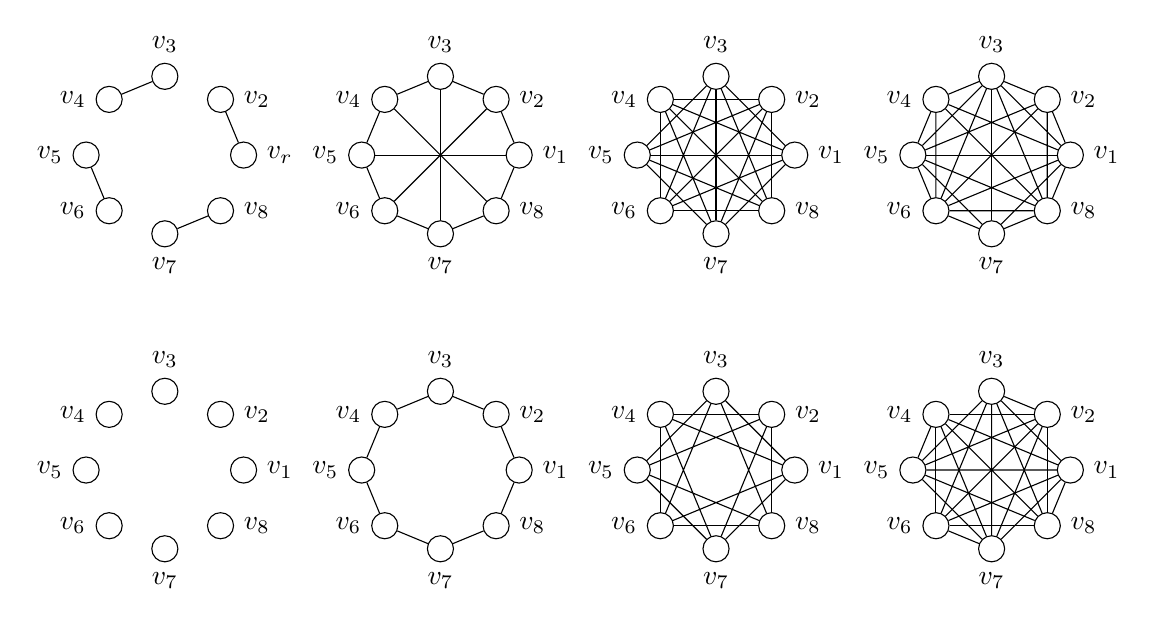
\begin{tikzpicture}[scale=0.5]
		\draw (0,0) node (a)[circle]{};
		\draw (a) ++(0:2) node (a1)[draw,circle,label=right:$v_1$]{};
		\draw (a) ++(45:2) node (a2)[draw,circle,label=right:$v_2$]{};
		\draw (a) ++(90:2) node (a3)[draw,circle,label=above:$v_3$]{};
		\draw (a) ++(135:2) node (a4)[draw,circle,label=left:$v_4$]{};
		\draw (a) ++(180:2) node (a5)[draw,circle,label=left:$v_5$]{};
		\draw (a) ++(225:2) node (a6)[draw,circle,label=left:$v_6$]{};
		\draw (a) ++(-90:2) node (a7)[draw,circle,label=below:$v_7$]{};
		\draw (a) ++(-45:2) node (a8)[draw,circle,label=right:$v_8$]{};

		\draw (0,8) node (b)[circle]{};
		\draw (b) ++(0:2) node (b1)[draw,circle,label=right:$v_r$]{};
		\draw (b) ++(45:2) node (b2)[draw,circle,label=right:$v_2$]{};
		\draw (b) ++(90:2) node (b3)[draw,circle,label=above:$v_3$]{};
		\draw (b) ++(135:2) node (b4)[draw,circle,label=left:$v_4$]{};
		\draw (b) ++(180:2) node (b5)[draw,circle,label=left:$v_5$]{};
		\draw (b) ++(225:2) node (b6)[draw,circle,label=left:$v_6$]{};
		\draw (b) ++(-90:2) node (b7)[draw,circle,label=below:$v_7$]{};
		\draw (b) ++(-45:2) node (b8)[draw,circle,label=right:$v_8$]{};
		\draw (b1)--(b2);
		\draw (b3)--(b4);
		\draw (b5)--(b6);
		\draw (b7)--(b8);

		\draw (7,0) node (c)[circle]{};
		\draw (c) ++(0:2) node (c1)[draw,circle,label=right:$v_1$]{};
		\draw (c) ++(45:2) node (c2)[draw,circle,label=right:$v_2$]{};
		\draw (c) ++(90:2) node (c3)[draw,circle,label=above:$v_3$]{};
		\draw (c) ++(135:2) node (c4)[draw,circle,label=left:$v_4$]{};
		\draw (c) ++(180:2) node (c5)[draw,circle,label=left:$v_5$]{};
		\draw (c) ++(225:2) node (c6)[draw,circle,label=left:$v_6$]{};
		\draw (c) ++(-90:2) node (c7)[draw,circle,label=below:$v_7$]{};
		\draw (c) ++(-45:2) node (c8)[draw,circle,label=right:$v_8$]{};
		\draw (c1)--(c2)--(c3)--(c4)--(c5)--(c6)--(c7)--(c8)--(c1);

		\draw (7,8) node (d)[circle]{};
		\draw (d) ++(0:2) node (d1)[draw,circle,label=right:$v_1$]{};
		\draw (d) ++(45:2) node (d2)[draw,circle,label=right:$v_2$]{};
		\draw (d) ++(90:2) node (d3)[draw,circle,label=above:$v_3$]{};
		\draw (d) ++(135:2) node (d4)[draw,circle,label=left:$v_4$]{};
		\draw (d) ++(180:2) node (d5)[draw,circle,label=left:$v_5$]{};
		\draw (d) ++(225:2) node (d6)[draw,circle,label=left:$v_6$]{};
		\draw (d) ++(-90:2) node (d7)[draw,circle,label=below:$v_7$]{};
		\draw (d) ++(-45:2) node (d8)[draw,circle,label=right:$v_8$]{};
		\draw (d1)--(d2)--(d3)--(d4)--(d5)--(d6)--(d7)--(d8)--(d1);
		\draw (d1)--(d5);
		\draw (d2)--(d6);
		\draw (d3)--(d7);
		\draw (d4)--(d8);

		\draw (14,0) node (e)[circle]{};
		\draw (e) ++(0:2) node (e1)[draw,circle,label=right:$v_1$]{};
		\draw (e) ++(45:2) node (e2)[draw,circle,label=right:$v_2$]{};
		\draw (e) ++(90:2) node (e3)[draw,circle,label=above:$v_3$]{};
		\draw (e) ++(135:2) node (e4)[draw,circle,label=left:$v_4$]{};
		\draw (e) ++(180:2) node (e5)[draw,circle,label=left:$v_5$]{};
		\draw (e) ++(225:2) node (e6)[draw,circle,label=left:$v_6$]{};
		\draw (e) ++(-90:2) node (e7)[draw,circle,label=below:$v_7$]{};
		\draw (e) ++(-45:2) node (e8)[draw,circle,label=right:$v_8$]{};
		%\draw (e1)--(e2)--(e3)--(e4)--(e5)--(e6)--(e7)--(e8)--(e1);
		\draw (e1)--(e3)--(e5)--(e7)--(e1);
		\draw (e2)--(e4)--(e6)--(e8)--(e2);
		\draw (e1)--(e4)--(e7)--(e2)--(e5)--(e8)--(e3)--(e6)--(e1);

		\draw (14,8) node (f)[circle]{};
		\draw (f) ++(0:2) node (f1)[draw,circle,label=right:$v_1$]{};
		\draw (f) ++(45:2) node (f2)[draw,circle,label=right:$v_2$]{};
		\draw (f) ++(90:2) node (f3)[draw,circle,label=above:$v_3$]{};
		\draw (f) ++(135:2) node (f4)[draw,circle,label=left:$v_4$]{};
		\draw (f) ++(180:2) node (f5)[draw,circle,label=left:$v_5$]{};
		\draw (f) ++(225:2) node (f6)[draw,circle,label=left:$v_6$]{};
		\draw (f) ++(-90:2) node (f7)[draw,circle,label=below:$v_7$]{};
		\draw (f) ++(-45:2) node (f8)[draw,circle,label=right:$v_8$]{};
		\draw (f1)--(f3)--(f5)--(f7)--(f1);
		\draw (f2)--(f4)--(f6)--(f8)--(f2);
		\draw (f1)--(f4)--(f7)--(f2)--(f5)--(f8)--(f3)--(f6)--(f1);
		\draw (f1)--(f5);
		\draw (f2)--(f6);
		\draw (f3)--(f7);
		\draw (f4)--(f8);

		\draw (21,0) node (g)[circle]{};
		\draw (g) ++(0:2) node (g1)[draw,circle,label=right:$v_1$]{};
		\draw (g) ++(45:2) node (g2)[draw,circle,label=right:$v_2$]{};
		\draw (g) ++(90:2) node (g3)[draw,circle,label=above:$v_3$]{};
		\draw (g) ++(135:2) node (g4)[draw,circle,label=left:$v_4$]{};
		\draw (g) ++(180:2) node (g5)[draw,circle,label=left:$v_5$]{};
		\draw (g) ++(225:2) node (g6)[draw,circle,label=left:$v_6$]{};
		\draw (g) ++(-90:2) node (g7)[draw,circle,label=below:$v_7$]{};
		\draw (g) ++(-45:2) node (g8)[draw,circle,label=right:$v_8$]{};
		\draw (g1)--(g3)--(g5)--(g7)--(g1);
		\draw (g2)--(g4)--(g6)--(g8)--(g2);
		\draw (g1)--(g4)--(g7)--(g2)--(g5)--(g8)--(g3)--(g6)--(g1);
		\draw (g1)--(g5)--(g4)--(g8)--(g1);
		\draw (g2)--(g3)--(g7)--(g6)--(g2);

		\draw (21,8) node (h)[circle]{};
		\draw (h) ++(0:2) node (h1)[draw,circle,label=right:$v_1$]{};
		\draw (h) ++(45:2) node (h2)[draw,circle,label=right:$v_2$]{};
		\draw (h) ++(90:2) node (h3)[draw,circle,label=above:$v_3$]{};
		\draw (h) ++(135:2) node (h4)[draw,circle,label=left:$v_4$]{};
		\draw (h) ++(180:2) node (h5)[draw,circle,label=left:$v_5$]{};
		\draw (h) ++(225:2) node (h6)[draw,circle,label=left:$v_6$]{};
		\draw (h) ++(-90:2) node (h7)[draw,circle,label=below:$v_7$]{};
		\draw (h) ++(-45:2) node (h8)[draw,circle,label=right:$v_8$]{};
		\draw (h1)--(h2)--(h3)--(h4)--(h5)--(h6)--(h7)--(h8)--(h1);
		\draw (h1)--(h3)--(h5)--(h7)--(h1)--(h4)--(h6)--(h8)--(h2)--(h5)--(h8)--(h3)--(h6)--(h1);
		\draw (h1)--(h5);
		\draw (h2)--(h6);
		\draw (h3)--(h7);
		\draw (h4)--(h8);
	\end{tikzpicture}
	\caption{$r$-regular graph of order $8$}
	\label{dia:regularOrder8}
	\end{figure}
\item Determine the complement of each graph constructed in (a).\\
	(complements are already there in the list)
	\item Prove that if $G$ is a regular graph. Then $\bar{G}$ is regular.
	\begin{proof}
	Let $G$ be an $r$-regular graph of order $p$. Let $v \in V(G)$. Then $deg\ v = r$. Thus, there are $r$ vertices adjacent to $v$ in graph $G$. In other words, there are $p-r-1$ vertices non-adjacent to $v$ in $G$. Therefore, $deg\ v$ is the complement graph $\bar{G}$ is $p-r-1$. Since $v \in V(G)$ is arbitrary, $\bar{G}$ is $p-r-1$-regular graph.
	\end{proof}
\end{enumerate}
\end{enumerate}

\section{Isomorphic Graphs}
\begin{definition}[isomorphism]
	Two graphs $G_1,G_2$ are isomorphic if there exists a bijection $$\phi : V(G_1) \to V(G_2) \text{ such that }uv \in E(G_1) \iff \phi(u)\phi(v) \in E(G_2)$$
\end{definition}
\begin{remark}
	Two graphs $G_1,G_2$ are equal if $V(G_1) = V(G_2)$ and $E(G_1) = E(G_2)$. Clearly, equal graphs are isomorphic. However, isomorphic graphs are not equal.
\end{remark}

\subsection*{Problem Set 1.3}
\begin{enumerate}
	\item Find two non-isomorphic $3$-regualr graphs of order $6$ and size $9$.\\
		There are exactly two non-isomorphic $3$-regular graphs of order $6$. By first theorem of graph theory, the size of such a graph is always $9$.(see Figure \ref{dia:3r6o}.
	\begin{figure}[hbt]
		\centering
		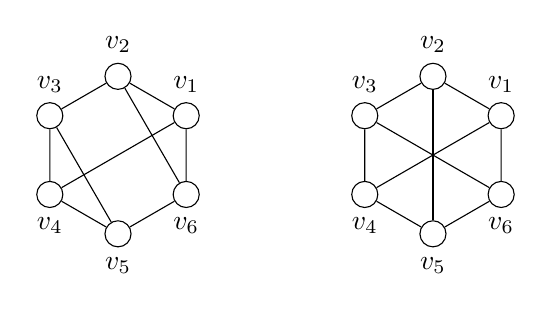
\begin{tikzpicture}[scale=0.5]
			\draw (8,0) node (v){};
			\draw (v) ++(30:2) node (v1)[draw,circle,label=above:$v_1$]{};
			\draw (v) ++(90:2) node (v2)[draw,circle,label=above:$v_2$]{};
			\draw (v) ++(150:2) node (v3)[draw,circle,label=above:$v_3$]{};
			\draw (v) ++(-150:2) node (v4)[draw,circle,label=below:$v_4$]{};
			\draw (v) ++(-90:2) node (v5)[draw,circle,label=below:$v_5$]{};
			\draw (v) ++(-30:2) node (v6)[draw,circle,label=below:$v_6$]{};
			\draw (v1)--(v2)--(v3)--(v4)--(v5)--(v6)--(v1);
			\draw (v1)--(v4);
			\draw (v2)--(v5);
			\draw (v3)--(v6);

			\draw (0,0) node (u){};
			\draw (u) ++(30:2) node (u1)[draw,circle,label=above:$v_1$]{};
			\draw (u) ++(90:2) node (u2)[draw,circle,label=above:$v_2$]{};
			\draw (u) ++(150:2) node (u3)[draw,circle,label=above:$v_3$]{};
			\draw (u) ++(-150:2) node (u4)[draw,circle,label=below:$v_4$]{};
			\draw (u) ++(-90:2) node (u5)[draw,circle,label=below:$v_5$]{};
			\draw (u) ++(-30:2) node (u6)[draw,circle,label=below:$v_6$]{};
			\draw (u1)--(u2)--(u3)--(u4)--(u5)--(u6)--(u1);
			\draw (u1)--(u4);
			\draw (u2)--(u6);
			\draw (u3)--(u5);
		\end{tikzpicture}
		\caption{$3$-regular graph of order $6$}
		\label{dia:3r6o}
	\end{figure}
	\item
	\begin{enumerate}
	\item Draw all eleven nonisomorphic graphs of order $4$\\
		$P_4,C_4,\bar{C_4},K_4,\bar{K_4},K_4-e,K_2+2K_1,K_{1,3},\bar{K}_{1,3},P_2+K_1,C_3+e$
	\item Let $S$ be a set of $23$ graphs of order $4$, then $S$ has at least three graphs that are pairwise isomorphic.
	\begin{proof}
		There are at most eleven non-isomorphic graphs of order $r$.
		By pigeonhole principle, in a family of $23$ graphs of order $4$ at least three graphs are pairwise isomorphic.
	\end{proof}
	\end{enumerate}
	\item Give an example of a graph $G$ of order $5$ such that $G \cong \bar{G}$.\\
		There are only two such graphs upto isomorphism.(see Figure \ref{dia:sc5})
	\begin{figure}[hbt]
	\centering
	\begin{tikzpicture}
		\draw (0,0) node (u){};
		\draw (u) ++(36:2) node (u1)[draw,circle,label=right:$v_1$]{};
		\draw (u) ++(108:2) node (u2)[draw,circle,label=above:$v_2$]{};
		\draw (u) ++(180:2) node (u3)[draw,circle,label=left:$v_3$]{};
		\draw (u) ++(-108:2) node (u4)[draw,circle,label=above:$v_4$]{};
		\draw (u) ++(-36:2) node (u5)[draw,circle,label=right:$v_5$]{};
		\draw (u1)--(u2)--(u3)--(u4)--(u5);
		\draw (u2)--(u4);

		\draw (6,0) node (v){};
		\draw (v) ++(36:2) node (v1)[draw,circle,label=right:$v_1$]{};
		\draw (v) ++(108:2) node (v2)[draw,circle,label=above:$v_2$]{};
		\draw (v) ++(180:2) node (v3)[draw,circle,label=left:$v_3$]{};
		\draw (v) ++(-108:2) node (v4)[draw,circle,label=above:$v_4$]{};
		\draw (v) ++(-36:2) node (v5)[draw,circle,label=right:$v_5$]{};
		\draw (v1)--(v2)--(v3)--(v4)--(v5)--(v1);
	\end{tikzpicture}
	\caption{Self-complementary graphs of order $5$}
	\label{dia:sc5}
	\end{figure}
	\item There are three regular graphs of order $5$, and eight regular graphs of order $6$. Draw all of them\\
		Three regular graphs of order $5$ are $C_5,K_5$ and $\bar{K}_5$.\\
		Eight regular graphs of order $6$ are $3K_2,C_6,2K_3,K_6$ and complements.
	\item Prove that two graph $G_1$ and $G_2$ are isomorphic if and only if their complements are isomorphic.
	\begin{proof}
	\begin{align*}
	G_1 \cong G_2 
		& \iff \phi : G_1 \to G_2,\ \left[uv \in E(G_1) \iff  \phi(u)\phi(v) \in E(G_2)\right] \\
		& \iff \phi : G_1 \to G_2,\ \left[uv \notin E(G_1) \iff \phi(u)\phi(v) \notin E(G_2)\right] \\
		& \iff \bar{G}_1 \cong \bar{G}_2
	\end{align*}
	\end{proof}
	\item Draw all nonisomorphic $4$-regular graphs of order $7$.\\
		There are only two distinct $2$-regular graphs of order $7$ upto isomorphism. The graphs are $C_7$ and $C_3+C_4$. Every $4$-regular graphs of order $7$ is complement of some $2$-regular graph of order $7$. Thus there are only two $4$-regular graphs of order $7$. The graphs are $\bar{C}_7$ and $\overline{C_3+C_4}$.

\begin{commentary}
	There are two trivial regular graphs $K_p$ and $\bar{K}_p$. In order to count regular graphs of order $p$, it is always easier to count $r$-regular graphs for $0 \le r \le \lfloor (p-1)/2 \rfloor$.\\

	For example, $p=8$. We need to construct all nonisomorphic $r$-regular graphs of order $8$ for $r=0,1,2,3$. There are one graph each for $r=0,1$. The $2$-regular graphs are always disjoint union of cycles. Thus, the only possibilities are $C_3+C_5, 2C_4$ and $C_8$. Finding $3$-regular graphs of order $8$ is the hard part.\\

	You may find various classifications of all small graphs (upto order $13$) at \href{https://www.graphclasses.org/smallgraphs.html}{graphclasses.org}. And there is a combinatorial result on number of regular graphs of order $p$ available at \href{https://oeis.org/A051031}{oeis.org}.\\

	As per OEIS there are six nonisomorphic $3$ regular graph of order $8$. Thus, there are twenty two nonisomophic regular graphs of order $8$.
\end{commentary}
	\setcounter{enumi}{8}
	\item Show that the relation `is isomorphic to' is an equivalence relation on the set of all graphs.
	\begin{proof}
		Trivially $G \cong G$ as $G$ is equal to itself and equal graphs are always isomorphic.\\

		Suppose $G_1 \cong G_2$. Then there exists a bijection $\phi : V(G_1) \to V(G_2)$ such that $uv \in E(G_1) \iff \phi(u)\phi(v) \in E(G_2)$. Clearly, $\phi^{-1} : V(G_2) \to V(G_1)$ is an isomorphism. Thus, $G_2 \cong G_1$.\\

		Suppose $G_1 \cong G_2$ and $G_2 \cong G_3$.
		Then there exist bijection $\phi : V(G_1) \to V(G_2)$ such that $uv \in E(G_1) \iff \phi(u)\phi(v) \in E(G_2)$ and bijection $\psi : V(G_2) \to V(G_3)$ such that
		$$\phi(u)\phi(v) \in E(G_2) \iff \psi(\phi(u))\psi(\phi(v)) \in E(G_3)$$
		Clearly, $\psi \circ \phi : V(G_1) \to V(G_3)$ is a bijection such that
		$$ uv \in E(G_1) \iff \psi \circ \phi(u) \psi\circ\phi(v) \in E(G_3) $$
		Therefore, $G_1 \cong G_3$.
	\end{proof}
\end{enumerate}
\section{Subgraphs}
---to continue-- (pp. 12)
\section{Degree Sequences}
\section{Connected Graphs}
\section{Cut-Vertices and Bridges}
\section{Special Graphs}
\section{Digraphs}

%\chapter{An Introduction to Algorithms}
\section{Algorithmic Complexity}
\section{Serach Algorithms}
\section{Sorting Algorithms}
%\section{Introducing NP-Completeness*}
\setcounter{section}{4}
\section{Greedy Algorithms}
\section{Representing Graphs in a Computer}

%Module 2
%\chapter{Trees}
\section{Properties of Trees}
\section{Rooted Trees}
\section{Depth-First Search}
\section{Depth-First Search : A Tool for Finding Blocks}
\section{Breadth-First Search}
\section{The Minimum Spanning Tree Problem}

%\chapter{Paths and Distance in Graphs}
\section{Distance in Graphs}
\section{Distance in Weighted Graphs}
\section{The Center and Median of a Graph}
\section{Activity Digraphs and Critical Paths}
%\section{Error Correcting Codes$^\ast$}

%Module 3
\section{Networks}
\subsection{An Introduction to Networks}
\begin{definition}
	A \textbf{network} $N$ is a digraph $D$ with two special vertices source $s$ and sink $t$ together with a capacity function $c : E(D) \to \mathbb{Z}$ such that for every arc $a = (u,v)$ of the digraph, $c(u,v)$ is non-negative.
\end{definition}

\begin{remark} Mathematical Modeling using Network,
	\begin{enumerate}
		\item There is no restriction on indegree/outdegree of source/sink vertices of the digraph $D$ of a network $N$.
		\item Applications of Network : Transportation problem.
	\end{enumerate}
\end{remark}

\begin{description}
	\item[$c(u,v)$] is the capacity of the arc $(u,v)$ of $D$
	\item[$N^+(x)$] $= \{ y \in V(D) : (x,y) \in E(D)\}$ is the out-neighbourhood of $x$.
	\item[$N^-(x)$] $= \{ y \in V(D) : (y,x) \in E(D)\}$ is the in-neighbourhood of $x$.
\end{description}

\begin{definition}
	A \textbf{flow f in a network N} is function $f : E(D) \to \mathbb{Z}$ such that
	\begin{enumerate*}
		\item each edge satisfies capacity constraint and
		\item each vertex except source and sink satisfies conservation equation.
	\end{enumerate*}
\end{definition}

\begin{description}
	\item[capacity constraint] 
		\begin{equation}
		0 \le f(a) \le c(a) \text{ for every arc }a \in V(D)
		\end{equation}
	\item[conservation equation] 
		\begin{equation}
			\sum_{y \in N^+(x)} f(x,y) = \sum_{y \in N^-(x)} f(y,x),\ \forall \text{vertex } x \in V(D)-\{s,t\}
		\label{equ:conservation}
		\end{equation}
	\item[net flow out of $x$]
		\[ \sum_{y \in N^+(x)} f(x,y) - \sum_{y \in N^-(x)} f(y,x) \]
	\item[net flow into $x$]
		\[ \sum_{y \in N^-(x)} f(y,x) - \sum_{y \in N^+(x)} f(x,y) \]
\end{description}

\begin{definition}
	The \textbf{flow f in a network N} is the net flow out of source $s$.
\end{definition}

\begin{remark}
	\begin{enumerate}
		\item net flow out of/into $x \in V(D)-\{s,t\}$ is zero.
		\item Without loss of generality\footnote{If underlying digraph of a network is symmetric, then by replacing an arc $(u,v)$ with a new vertex $w$ and two arcs $(u,w),(w,v)$ gives an assymetric digraph.\cite{chartrand}pp.131}, underlying digraph is always assymetric.
	\end{enumerate}
\end{remark}

\begin{description}
	\item[$(X,Y)$] $=\{ (x,y) \in E(D) : x \in X,\ y \in Y \}$.\\
		Let $X,Y$ be non-empty subsets of $V(D)$ such that $X,Y$ are disjoint.
		Then $(X,Y)$ is the set of all arcs from $X$ to $Y$.
	\item[flow from $X$ to $Y$] is the sum of flow on each arc in $(X,Y)$
		\begin{equation}
		f(X,Y) = \sum_{(x,y) \in (X,Y)} f(x,y)
		\end{equation}
	\item[capacity of the partition $(X,Y)$] is the total capacity of arcs in $(X,Y)$
		\begin{equation}
		c(X,Y) = \sum_{(x,y) \in (X,Y)} c(x,y)
		\end{equation}
	\item[cut] Let $P \subset V(D)$ such that $s \in P$ and $t \notin P$ and $\bar{P} = V(D)-P$, then $(P,\bar{P})$ is a cut.
	\item[flow from $P$ to $\bar{P}$] is the sum of flow on each arc in $(P,\bar{P})$.
		\begin{equation}
		f(P,\bar{P}) = \sum_{(x,y) \in (P,\bar{P})} f(x,y)
		\end{equation}
	\item[flow from $\bar{P}$ to $P$] is the sum of flow on each arc in $(\bar{P},P)$
		\begin{equation}
		f(\bar{P},P) = \sum_{(x,y) \in (\bar{P},P)} f(x,y)
		\end{equation}
	\item[capacity of the cut $(P,\bar{P})$] is the total capacity of the arcs in $(P,\bar{P})$
		\begin{equation}
		c(P,\bar{P}) = \sum_{(x,y) \in (P,\bar{P})} c(x,y)
		\end{equation}
\end{description}

\begin{theorem}
	For any cut $(P,\bar{P})$, the flow in $N$ is $f(N) = f(P,\bar{P}) - f(\bar{P},P)$.
\end{theorem}
\begin{synopsis}
	The net flow out of source $s$ is the flow $f(N)$ in the network $N$.
	Let $(P,\bar{P})$ be a cut of $N$, then $s \in P$ and $t \notin P$.
	Suppose $P = \{ s\}$, then the theorem is true.
	Suppose $P$ is not singleton, then for each vertex $x \in P,\ x \ne s$, the net flow out of $x$ is zero by flow conservation equation.
	And flow between vertices in $P$ cancels out each other.
	Thus adding net flow out of each vertex in $P$, will be same as the net flow out of source which is the flow in the network, $f(N)$.
\end{synopsis}
\begin{proof}
	\begin{equation}
		\text{Flow, }f = \sum_{y \in N^+(s)} f(s,y) - \sum_{y \in N^-(s)} f(y,s)
	\end{equation}
	By conservation equation, we have $\forall x \in P,\ x \ne s$,
	\begin{equation}
		\sum_{y \in N^+(x)} f(x,y) - \sum_{y \in N^-(x)} f(y,x) = 0
	\end{equation}
	By above equations,
	\begin{align}
		\text{Flow, } f & = \sum_{x \in P} \sum_{y \in N^+(x)} f(x,y) - \sum_{x \in P} \sum_{y \in N^-(x)} f(y,x) \nonumber\\
				& = \sum_{(x,y) \in (P,\bar{P})} f(x,y) - \sum_{(y,x) \in (\bar{P},P)} f(y,x) 
	\end{align}
\end{proof}

\begin{corollary}
	Flow cannot exceed the capacity of any cut $(P,\bar{P})$.
	Further, $f(N) \le \min c(P,\bar{P})$.
\end{corollary}
\begin{synopsis}
	Let $(P,\bar{P})$ be a cut in network $N$, then by theorem the flow $f(N) =$  flow from $P$ to $\bar{P}$ - flow from $\bar{P}$ to $P$.
	Since the flow from $\bar{P}$ to $P$ is non-negative, $f(N) \le$ flow from $P$ to $\bar{P}$.
	Clearly, $f(x,y) \le c(x,y)$ by the capacity constaint.
	Thus $f(N) \le f(P,\bar{P}) \le c(P,\bar{P}) \le \min c(P,\bar{P})$.
\end{synopsis}
\begin{proof}
	\begin{align*}
		f(N) 	& = \sum_{(x,y) \in (P,\bar{P})} f(x,y) - \sum_{(y,x) \in (\bar{P},P)} f(y,x) \\
			& \le \sum_{(x,y) \in (P,\bar{P})} f(x,y) = f(P,\bar{P})\\ 
			& \le \sum_{(x,y) \in (P,\bar{P})} c(x,y) = c(P,\bar{P}),\quad \because \forall x,y \in V(D),\ f(x,y) \le c(x,y) \\
			& \le \min c(P,\bar{P})
	\end{align*}
\end{proof}

\begin{corollary}
	In a network $N$ flow is the net flow into the sink of $N$.
\end{corollary}
\begin{synopsis}
	Let $\bar{P} = \{ t \}$, then by theorem $f(N)$ is the net flow into the sink.
\end{synopsis}
\begin{proof}
	Suppose $P = V(D)-\{t\}$.
	Then by theorem, we have
	\begin{align*}
		f(N) 	& = \sum_{(x,y) \in (P,\bar{P})} f(x,y) - \sum_{(y,x) \in (\bar{P},P)} f(y,x) \\
			& = \sum_{x \in N^-(t)} f(x,t) - \sum_{x \in N^+(t)} f(t,x)
	\end{align*}
\end{proof}

\begin{remark}Exercise 5.1
	\begin{enumerate}
		\setcounter{enumi}{3}
		\item Let $N$ be a network with underlying digraph $D$ which has a vertex $v \in V(D) - \{ s,t \}$ with zero indegree.
			Clearly the flow into $v$ is zero.
			Thus flow out of $v$ is also zero by flow conservation equation.
			Let $N'$ be the network obtained from $N$ by deleting the vertex $v$.
			Then $f(N) = f(N')$.
	\end{enumerate}
\end{remark}

\subsection{The Max-Flow Min-Cut Theorem}
\begin{description}
	\item[maximum flow] A flow $f$ in network $N$ is maximum flow in $N$, if $f(N) \ge f'(N)$ for each flow $f'$ in $N$.
	\item[minimum cut] A cut $(P,\bar{P})$ in network $N$ is minimum cut of $N$,\\ if $c(P,\bar{P}) \le c(X,\bar{X})$ for each cut $(X,\bar{X})$ in $N$.
	\item[$f$-unsaturated] Let $f$ be a flow in network $N$ with underlying digraph $D$, and $Q = u_0,a_1,u_1,a_2,\cdots,u_{n-1},a_n,u_n$ be a semipath in $D$ such that every forward arc $a_i = (u_{i-1},u_i)$ has flow not upto its capacity, $f(a_i) < c(a_i)$ and every reverse arc $a_i = (u_i,u_{i-1})$ has some positive flow in it, $f(a_i) > 0$
	\item[f-augmenting semipath] Let $f$ be a flow in a network $N$ with underlying digraph $D$.
		Suppose semipath $Q = s,a_1,u_1,a_2,\cdots,u_{n-1},a_n,t$ (from source to sink) is $f$-unsaturated, then $Q$ is an $f$-augmenting semipath.
\end{description}

\begin{theorem}
	Let $f$ be a flow in a network $N$ with underlying digraph $D$.
	The flow $f$ is maximum in $N$ iff there is no $f$-augmenting semipath in $D$.
\end{theorem}
\begin{synopsis}
	Suppose $Q$ is an $f$-augmenting semipath in $D$, then there exists a flow $f^*$ in $N$ such that $f(N)+\Delta = f^*(N)$.
	Therefore, $f$ is not a maximum flow in $N$.
	Suppose there is no $f$-augmenting semipath in $D$, then there exists a cut $(P,\bar{P})$ such that $f(a) = c(a)\ \forall a \in (P,\bar{P})$ and $f(a) = 0\ \forall a \in (\bar{P},P)$.
	Suppose $f^*$ in a maximum flow in $N$, then $f(N) \le f^*(N) \le c(P,\bar{P}) = f(N)$.
\end{synopsis}
\begin{proof}
	Let $f$ be a flow in a network $N$ with underlying digraph $D$ and $Q = s, a_1, u_1, a_2, u_2, \cdots, u_{n-1}, a_n, t$ be an $f$-augmenting semipath in $D$.
	\[\text{define } \Delta_i = \begin{cases}
		c(a_i) - f(a_i) \text{ for every forward arc } a_i \in Q, \\
		f(a_i) \text{ for every reverse arc } a_i \in Q,
	\end{cases} \]
	Define $\Delta = \min \{ \Delta_i \}$.
	Also define $f^* : E(D) \to \mathbb{Z}$ such that 
	\[ f^*(a_i) = \begin{cases} f(a) + \Delta \text{, for every forward arc } a_i \in Q, \\
	f(a) - \Delta \text{, for every reverse arc } a_i \in Q, \\
	f(a_i) \text{, for every arc of } D \text{ which are not in }Q.
	\end{cases} \]
		Since $Q$ is an $f$-augmenting semipath in $D$, $\Delta > 0$ and $f(N) + \Delta = f^*(N)$.\\

	Clearly $f(N) < f^*(N)$, and it is enough to show that $f^*$ is a flow in $N$.
$f^*$ is a flow if it satisfies \begin{enumerate*} \item capacity constraint and \item conservation equation \end{enumerate*}.
			For any arc $a_i \notin Q$, $f^*(a_i) = f(a_i) \le c(a_i)$.
			Suppose $a_i \in Q$.
			If $a_i = (u_{i-1},u_i)$, $a_i$ is a forward arc and we have $f^*(a_i) = f(a_i) + \Delta \le f(a_i) + \Delta_i = f(a_i) + c(a_i) - f(a_i) = c(a_i)$.
			If $a_i = (u_i,u_{i-1})$, then $a_i$ is a reverse arc and we have $f^*(a_i) = \Delta \le \min \{ \Delta_i \} = \Delta_i = c(a_i)$.
			Thus $f^*$ satisfies capactity constraint on every arc of $D$.\\

	Let $x \in V(D)-\{s,t\}$.
	Suppose $x \notin Q$,
	\begin{align*}
		\text{Net flow out of } x
		& = \sum_{y \in N^+(x)} f^*(x,y) - \sum_{y \in N^-(x)} f^*(y,x) \\
		& = \sum_{y \in N^+(x)} f(x,y) - \sum_{y \in N^-(x)} f(y,x) \\
		& = 0
	\end{align*}
	
	Suppose $x = u_i \in Q$, then $Q$ has two arc having vertex $x$ say, $a_{i-1}$, and $a_i$.
	There are four possibilities for these two arcs,
	\begin{enumerate}
		\item Both $a_{i-1},\ a_i$ are forward arcs.
		\item Arc $a_{i-1}$ is forward, but arc $a_i$ is reverse.
		\item Arc $a_{i-1}$ is reverse, but arc $a_i$ is forward.
		\item Both $a_{i-1},\ a_i$ are reverse arcs.
	\end{enumerate}
	
	\paragraph{Case 1} $a_{i-1} = (u_{i-1},u_i)$ and $a_i = (u_i, u_{i+1})$.
	\begin{align*}
		\text{ Net flow out of } x
		& = \sum_{y \in N^+(x)} f^*(x,y) - \sum_{y \in N^-(x)} f^*(y,x)\\
		& = \sum_{\frac{y \in N^+(x)}{y \ne u_{i+1}}} f^*(x,y) + f^*(u_i,u_{i+1}) - \left( \sum_{\frac{y \in N^-(x)}{y \ne u_{i-1}}} f^*(y,x) + f^*(u_{i-1},u_i) \right)\\
		& = \sum_{\frac{y \in N^+(x)}{y \ne u_{i+1}}} f(x,y) + f(u_i,u_{i+1}) + \Delta - \left( \sum_{\frac{y \in N^-(x)}{y \ne u_{i-1}}} f(y,x) + f(u_{i-1},u_i) \right) - \Delta \\
		& = \sum_{y \in N^+(x)} f(x,y) - \sum_{y \in N^-(x)} f(y,x) \\
		& = 0
	\end{align*}

	\paragraph{Case 2} $a_{i-1} = (u_{i-1},u_i)$ and $a_i = (u_{i+1},u_i)$.
	\begin{align*}
		\text{ Net flow out of } x
		& = \sum_{y \in N^+(x)} f^*(x,y) - \sum_{y \in N^-(x)} f^*(y,x) \\
		& = \sum_{\frac{y \in N^+(x)}{y \ne u_{i+1}, u_{i-1}}} f^*(x,y) + f^*(u_i,u_{i+1}) + f^*(u_i,u_{i-1}) - \sum_{y \in N^-(x)} f^*(y,x) \\
		& = \sum_{\frac{y \in N^+(x)}{y \ne u_{i+1}, u_{i-1}}} f(x,y) + f(u_i,u_{i+1}) + \Delta + f(u_i,u_{i-1}) - \Delta - \sum_{y \in N^-(x)} f(y,x) \\
		& = \sum_{y \in N^+(x)} f(x,y) - \sum_{y \in N^-(x)} f(y,x) \\
		& = 0
	\end{align*}

	\paragraph{Case 3} $a_{i-1} = (u_i, u_{i-1})$ and $a_i = (u_i,u_{i+1})$.
	\begin{align*}
		\text{ Net flow out of } x
		& = \sum_{y \in N^+(x)} f^*(x,y) - \sum_{y \in N^-(x)} f^*(y,x) \\
		& = \sum_{y \in N^+(x)} f^*(x,y) - \left( \sum_{\frac{y \in N^-(x)}{y \ne u_{i-1}, u_{i+1}}} f^*(y,x) + f^*(u_{i-1},u_i) + f^*(u_{i+1},u_i) \right)\\
		& = \sum_{y \in N^+(x)} f^*(x,y) - \left( \sum_{\frac{y \in N^-(x)}{y \ne u_{i-1}, u_{i+1}}} f(y,x) + f(u_{i-1},u_i) + \Delta + f(u_{i+1},u_i) - \Delta \right)\\
		& = \sum_{y \in N^+(x)} f(x,y) - \sum_{y \in N^-(x)} f(y,x) \\
		& = 0
	\end{align*}

	\paragraph{Case 4} $a_{i-1} = (u_i,u_{i-1})$ and $a_i = (u_{i+1},u_i)$.
	\begin{align*}
		\text{ Net flow out of } x
		& = \sum_{y \in N^+(x)} f^*(x,y) - \sum_{y \in N^-(x)} f^*(y,x) \\
		& = \sum_{\frac{y \in N^+(x)}{y \ne u_{i-1}}} f^*(x,y) + f^*(u_i,u_{i-1}) - \left( \sum_{\frac{y \in N^-(x)}{y \ne u_{i+1}}} f^*(y,x) + f^*(u_{i+1},u_i) \right)\\
		& = \sum_{\frac{y \in N^+(x)}{y \ne u_{i-1}}} f(x,y) + f(u_i,u_{i-1}) - \Delta - \left( \sum_{\frac{y \in N^-(x)}{y \ne u_{i+1}}} f(y,x) + f(u_{i+1},u_i) \right) + \Delta \\
		& = \sum_{y \in N^+(x)} f(x,y) - \sum_{y \in N^-(x)} f(y,x) \\
		& = 0
	\end{align*}
	Therefore, $f^*$ is a flow on $N$.
	We have $f(N) < f^*(N)$.
	Thus $f$ is not maximum flow in $N$ due to the existence of an $f$-augmenting semipath in $D$.

	\paragraph{}Conversely, assume that there is no $f$-augmenting semipath in $D$.
	Now, we construct a cut $(P,\bar{P})$ of $N$.
	Let $P$ be the set of all vertices $x \in V(D)$ such that there is an $f$-unsaturated $s-x$ semipath in $D$.
	Trivially, $s \in P$.
	And $t \notin P$ since there are no $f$-augmenting semipath in $D$.
	\footnote{An $f$-augmenting semipath is an $f$-unsaturated $s-t$ semipath in $D$.}
	Clearly, $(P,\bar{P})$ is a cut of the network $N$.\\


	We claim that $c(P,\bar{P}) = f(N)$.
	Suppose there is a forward arc $(x,y) \in (P,\bar{P})$, then flow in it is saturated.
	If $f(x,y) < c(x,y)$, then there is an $f$-unsaturated $s-y$ semipath in $D$.
	ie, $s-x$ semipath + arc $(x,y)$.
	Thus every forward arc $(x,y) \in (P,\bar{P})$ is saturated.
	Suppose there is a reverse arc $(y,x) \in (\bar{P},P)$, then there is no flow in it(saturated reversed arc).
	If $f(y,x) > 0$, then there is an $f$-unsaturated $s-y$ semipath in $D$.
	ie, $s-x$ semipath + arc $(y,x)$.
	Thus every reverse arc $(y,x) \in (\bar{P},P)$ is saturated.
	And we have,
	\begin{align*}
		\sum_{(x,y) \in (P,\bar{P})} f(x,y) & = \sum_{(x,y) \in (P,\bar{P})} c(x,y) \\
		\sum_{(y,x) \in (\bar{P},P)} f(y,x) & = 0 \\
		f(N) & = \sum_{(x,y) \in (P,\bar{P})} f(x,y) - \sum_{(y,x) \in (\bar{P},P)} f(y,x) \\
		& = \sum_{(x,y) \in (P,\bar{P})} c(x,y) \\
		& = c(P,\bar{P})
	\end{align*}

	Suppose $f^*$ is maximum flow in network $N$ and $(X,\bar{X})$ is minimum cut of $N$.
	Then $f(N) \le f^*(N)$.
	Thus we have, $f(N) \le f^*(N) \le c(X,\bar{X}) \le c(P,\bar{P}) = f(N)$.
	Therefore, $f(N) = f^*(N)$.
	ie, the flow $f$ is maximum in network $N$ if there are no $f$-augmenting semipaths in $D$.
\end{proof}

\begin{theorem}[maximum-flow, min-cut]
	In every network, the value of maximum flow equals capacity of minimum cut.
\end{theorem}
\begin{proof}
	Suppose flow $f$ in network $N$ in maximum, then by previous theorem there is no $f$-augmenting semipath in $D$.
	And $f(N) \le c(X,\bar{X})$ for any cut $(X,\bar{X})$ in $N$.
	We can construct a cut $(P,\bar{P})$ in $N$ such that $f(N) = c(P,\bar{P})$.
	Let $P$ be the set of all vertices $x$ in $D$ such that there is an $f$-unsaturated $s-x$ semipath in $D$.
	Clearly $s \in P$ and $t \notin P$.
	Also $f(P,\bar{P}) = c(P,\bar{P})$ and $f(\bar{P},P) = 0$.
	Then the cut $(P,\bar{P})$ is minimum cut of $N$.
	Suppose there is a cut $(X,\bar{X})$ such that $c(X,\bar{X}) < c(P,\bar{P})$.
	Then $f(N) = f(P,\bar{P}) - f(\bar{P},P) = c(P,\bar{P}) < c(X,\bar{X})$ which is a contradiction.
	Therefore, the value of maximum flow equals capacity of minimum cut.
\end{proof}

\begin{remark}Exercise 5.2
	\begin{enumerate}
		\item Suppose $(X,\bar{X})$ is a cut of $N$ such that $f(a) = c(a),\ \forall a \in (X,\bar{X})$ and $f(a) = 0,\ \forall a \in (\bar{X},X)$.
		By the definition of cut, $s \in X$ and $t \in \bar{X}$.
	Thus there is no $f$-augmenting semipath in $D$.
Suppose there is an $f$-augmenting semipath $Q$ in $D$, then there is either \begin{enumerate*} \item a forward arc $(x,y) \in (X,\bar{X})$ such that $f(x,y) < c(x,y)$ or \item a reverse arc $(y,x) \in (\bar{X},X)$ such that $f(y,x) > 0$ \end{enumerate*} which is a contradition.
			Therefore, the flow $f(N)$ is maximum and the given cut $(X,\bar{X})$ is minimum as shown in the proof of the maximum-flow min-cut theorem.
		\setcounter{enumi}{2}
	\item The algorithm suggested in the hint of this exercise won't work if two subnetworks have a common arc such that the direction of flow in which is not consistent.
		Suppose, the generalized network is not supposed to have any common arcs.
			Then construct subnetworks for each pair $(s,t)$ with all those arcs which are on some $s-t$ semipath.
			Define subnetwork capacity function $c'(a) = c(a)$ for every arc in $N'$.\\

	Let $N$ be a generalized network with set of sources $S$ and set of sinks $T$.
			A flow in $N$ is maximum if there is not $f$-augmenting $s-t$ semipath for each pair $(s,t) \in S \times T$.
%	Does there exists a generalised network where max-flow min-cut algorithm is inconsistent ? $\star$
	\end{enumerate}
\end{remark}

\subsection{A max-flow min-cut algorithm}
\begin{theorem}
	Let $N$ be a network with underlying digraph $D$, source $s$, sink $t$, capacity function $c$ and flow $f$.
	Let $D'$ be the digraph with same vertex set as $D$ and arc set defined by $E(D') = \{ (x,y) : (x,y) \in E(D),\ c(x,y) > f(x,y) \text{ or } (y,x) \in E(D),\ f(y,x) > 0 \}$.
	ie, $D'$ has only the unsaturated arcs of $D$.
	Then $D'$ has an $s-t$ directed path iff $D$ has an $f$-augmenting semipath.
	Moreover, shortest $s-t$ path in $D'$ has the same length as shortest $f$-augmenting semipath in $D$.
\end{theorem}
\begin{synopsis}
	Each directed $s-t$ path in $D'$ has respective $f$-augmenting semipath in $D$ and vice versa.
	Clearly, they have the same length.
\end{synopsis}
\begin{proof}
	Let $N$ be a network with underlying digraph $D$, capacity $c$ and flow $f$.
	Let $D'$ be the digraph with vertex set $V(D') = V(D)$ and arc set $E(D') = \{ (x,y) : \text{either }(x,y) \text{ or } (y,x) \text{ is unsaturated in } N \}$.\\


	Suppose $D'$ has a directed $s-t$ path $Q' : s,u_1,u_2,\cdots,u_{n-1},t$.
	Then by the construction of $D'$, for each $u_i \in Q$, there exists an $f$ unsaturated arc $a_i$ in $D$.
	ie, either forward arc $a_i = (u_{k-1},u_k)$ such that $f(u_{k-1},u_k) < c(u_{k-1},u_k)$ or reverse arc $a_i = (u_k,u_{k-1})$ such that $f(u_k,u_{k-1}) > 0$.
	Therefore, we have an $s-t$ semipath $Q : s,a_1,u_1,a_2,\cdots,u_{n-1},a_n,t$ in $D$ such that $Q$ is an $f$-augmenting semipath since every arc in $Q$ is $f$-unsaturated.
	Clearly, $Q,Q'$ are of the same length.\\


	Conversely, suppose that the digraph $D$ has an $f$-augmenting semipath $Q : s,a_1,u_1,a_2,\cdots,u_{n-1},a_n,t$.
	Then each arc $a_i \in Q$ are $f$-unsaturated and by the construction of $D'$, there exists a directed $s-t$ path $Q' = s,u_1,u_2,\cdots,u_{n-1},t$ in $D'$.
	And $Q,Q'$ are of the same length.\\


	There is a one-one correspondence betweeen the directed $s-t$ paths in $D'$ and $f$-augmenting semipaths in $D$.
	Clearly, they have the same length.
	Thus shortest directed $s-t$ path in $D$ and shortest $f$-augmenting semipath in $D'$ are of the same length.
\end{proof}

\begin{description}
	\item[saturation arc] of $N$ with respect to the flow $f$ is an arc $a_j$ in an $f$-augmenting semipath $Q$ with $\Delta_j = \Delta$.
	\item[augmentation path] is an $f$-augmenting semipath $Q$ in $D$.
\end{description}

\begin{algorithm}[max-flow min-cut]
	An algorithm to find maximum flow and minimum cut of a network $N$ with underlying digraph $D$, source $s$, sink $t$, capacity function $c$ and initial flow $f$.
	\begin{enumerate}
		\item Construct digraph $D'$ with vertex set $V(D') = V(D)$ and arc set $E(D') = \{ (x,y) : (x,y) \in E(D) \&  f(x,y) < c(x,y) \text{ or } (y,x) \in E(D) \& f(y,x) > 0 \}$
		\item Find (shortest) $s-t$ directed path in $D'$ using Moore's breadth first search(BFS) algorithm.
			If $D'$ doesn't have an $s-t$ path, then proceed to step 5.
			Otherwise, let $Q' : s,u_1,u_2,\cdots,u_{n-1},t$ be a (shortest) $s-t$ path in $D'$.
		\item Let $Q : s,a_1,u_1,a_2,\cdots,u_{n-1},a_n,t$ be the respective semipath in $D$ such that $f(a_j) < c(a_j)$ for forward arcs and $f(a_i) > 0$ for reverse arcs.
			Let $\Delta_j = c(a_j) - f(a_j)$ for forward arcs and $\Delta_j = f(a_j)$ for reverse arcs.
			And let $\Delta = \min \{ \Delta_j \}$.
			And augment flow $f$ by $\Delta$ ie, $f(a_j) \leftarrow f(a_j) + \Delta$ for forward arcs and $f(a_j) \leftarrow f(a_j)-\Delta$ for reverse arcs.
		\item Goto step 1 (Proceed with new flow $f$ and find whether there are any directed $s-t$ paths in $D'$.
			If any, augment the flow along the new augmentation path $Q$ by saturating the flow along the saturation arc.)
		\item There is no $s-t$ directed path in $D'$.
			Thus there is no $f$-augmenting semipath in $D$.
			Therefore the flow $f$ in $N$ is maximum.
			Let $P$ be the set of all vertices in $D'$ with non-zero breadth first index(bfi) from Moore's BFS algorithm applied in step 2.
			$(P,\bar{P})$ is minimum cut of $N$.
	\end{enumerate}
\end{algorithm}

\begin{remark}
	Validity of the algorithm is proved in the previous theorem.
\end{remark}

%\begin{remark}Exercises 5.3
%	\begin{enumerate}
%		\item
%		\item 
%		\item
%		\item
%	\end{enumerate}
%\end{remark}

%\section{The Complexity of the Max-Flow Min-Cut Theorem*}
\setcounter{subsection}{4}

\subsection{Connectivity and Edge-Connectivity}

\begin{description}
	\item[edge cutset] is the set $U$ subset of $E(G)$ such that $G-U$ is disconnected.
	\item[vertex cutset] is the set $S$ subset of $V(G)$ such that $G-S$ is disconnected.
	\item[edge connectivity] $\lambda(G)$ is the minimum cardinality of all edge cutsets of $G$.
	\item[connectivity] $\kappa(G)$ is the minimum cardinality of all vertex cutsets of $G$.
\end{description}

\begin{theorem}
	For every graph $G$, $\kappa(G) \le \lambda(G) \le \delta(G)$
\end{theorem}
\begin{proof}
	Suppose graph $G$ is disconnected then $\kappa(G) = \lambda(G) = \delta(G) = 0$.
	Let $G$ be a connected graph.
	Then $G$ has at least one vertex $v$ with degree $\delta(G)$.
	Therefore $\lambda(G) \le \delta(G)$ since edges incident with $v$ form an edge cutset of $G$ and $\lambda(G)$ is the cardinality of all edge cutsets.\\


	Let $G$ be a graph with edge connectivity $\lambda(G) = c$.
	Let $U$ be a edge cutset with cardinality $c$ and let edge $uv \in U$.
	Construct a set of vertices $S \subset V(G)$ such that ($S$ is of minimal cardinality and) for each edge in $U$ other $uv$, $S$ has a vertex incident with it.
	Cardinality of $S$ is atmost $c-1$, since we can select one vertex each for each edge in $U$ other than $u, v$.
	If $G-S$ is a disconnected graph, then $\kappa(G) < \lambda(G)$.
	Suppose $G-S$ is a connected graph, then delete a non-pendent vertex $u$ or $v$ from $G-S$, say $v$.
	Since $G-S$ is a connected graph with a singleton edge cutset, $\{ uv \}$.
	We have a vertex cutset $S \cup \{ v\}$ of $G$.
	Therefore, $\kappa(G) \le c = \lambda(G)$.
\end{proof}

\begin{theorem}
	If $G$ is a graph of diameter $2$, then $\lambda(G) = \delta(G)$
\end{theorem}
%\begin{proof}
%	Clearly $\lambda(G) \le \delta(G)$.
%	Therefore it is sufficient to prove that for a graph of diameter $2$, $\lambda(G) \not< \delta(G)$.
%	ie, for every non-trivial partition $X,Y$ of the vertex set $V(G)$, there are at least $\delta(G)$ edges between $X$ and $Y$.$\star$
%\end{proof}

\begin{description}
	\item[$n$-edge connected] $G$ is $n$-edge connected if $\lambda(G) \ge n$.
	\item[$n$ connected] $G$ is $n$-connected if $\kappa(G) \ge n$.
\end{description}

\begin{theorem}
	Let $G$ be a graph of order $p$ and $n$ be an integer such that $1 \le n \le p-1$.
	If $\delta(G) \ge \frac{p+n-2}{2}$, then $G$ is $n$-connected.
\end{theorem}
%\begin{proof}

%\end{proof}

\begin{description}
	\item[connection number] $c(G)$ is the smallest integer such that $2 \le c(G) \le p$ and every subgraph of order $n$ in $G$ is connected.
	\item[$l$-connectivity] $\kappa_l(G)$ is minimum number of vertices whose removal will produce a disconnected graph with at least $l$ components or a graph with fewer than $l$ vertices.
	\item[$(n,l)$-connected] A graph $G$ is $(n,l)$-connected if $\kappa_l(G) \ge n$.
\end{description}

\begin{remark}Exercises 5.5
	\begin{enumerate}
		\item $\lambda(K_{m,n}) = \kappa(K_{m,n}) = m$
		\setcounter{enumi}{7}
		\item $c(K_p) = 2$, $c(K_{m,n}) = n+1$, $c(C_p) = p-1$\\
			Every two vertices of complete graph of order $p$ are adjacent.
			For complete bi-partitie graph $K_{m,n}$ such that $1 \le m \le n$, there exists a totally disconnected subgraph of order $n$.
			Therefore $c(K_{m,n}) \ge n+1$.
			And with $n+1$ vertices, both partitions have at least two vertices each and therefore the graph is connected and $c(K_{m,n}) \le n+1$.
			For cycle $C_p$, any subgraph is disconnected if two non-adjacent vertices are deleted.
			Therefore $c(C_p) \ge p-1$.
			And $C_p$ remains connected even after deletion of any vertex, therefore $c(C_p) \le p-1$.
		\item
			\[ \delta(G) \ge \frac{p+(l-1)(n-2)}{l} \implies \kappa_l(G) \ge n \]
	\end{enumerate}
\end{remark}

\subsection{Menger's Theorem}
\begin{theorem}
	For a non-trivial graph $G$, $\lambda(u,v) = M'(u,v)$ for every pair $(u,v)$ of vertices of $G$.
\end{theorem}
\begin{corollary}
	Graph $G$ is $n$-edge connected iff every two vertices of $G$ are connected by at least $n$ edge disjoint paths.
\end{corollary}

\begin{theorem}
	For every pair of non-adjacent vertices $u,v$ in graph $G$, $\kappa(u,v) = M(u,v)$.
\end{theorem}
\begin{corollary}
	Graph $G$ is $n$-connected iff every pair of vertices of $G$ are connected by at least $n$ internally disjoint paths.
\end{corollary}

\begin{algorithm}[connectivity $\kappa(G)$].
	\begin{enumerate}
		\item If degree of every vertex is $p-1$, then output $\kappa = p-1$ and stop.
			Otherwise, continue.
		\item If $G$ is disconnected, output $\kappa = 0$ and stop.
			Otherwise, continue.
		\item $\kappa \leftarrow p$
		\item $i \leftarrow 0$
		\item If $i \le \kappa$, then $i \leftarrow i+1$ and continue.
			Otherwise, output $\kappa$ and stop.
		\item $j \leftarrow i+1$
		\item 
			\begin{enumerate}[label=(\arabic*)]
				\item If $j = p+1$, then return to step 5.
					Otherwise continue.
				\item If $v_iv_j \notin E(G)$, construct network $N$ with digraph $D$ as follows : for each vertex $ v \in V(G)$, there are two vertices $v',v'' \in V(D)$ and an arc $(v',v'') \in E(D)$.
					And for each edge $uv \in E(G)$, there are two arcs $(u'',v),(v'',u) \in E(D)$.
					The capacity function is given by, $c(v',v'') = 1$ for every $v \in V(G)$ and $c(a) = \infty$ for every other arc in $D$.
					Set source $s = v_i''$ and sink $t = v_j'$ and find maximum flow in $N$ using max-flow min-cut algorithm.
					Otherwise proceed to step 7d
				\item If $f(N) < \kappa$, then $\kappa \leftarrow f(N)$.
					Otherwise, continue.
				\item $j \leftarrow j+1$ and return to step 7a
			\end{enumerate}
	\end{enumerate}
\end{algorithm}

\section{Matchings and Factorizations}
\subsection{An Introduction to Matching}
\begin{description}
	\item[Marriage Problem] Given a collection of men and women, where each womon knows some of the men.
		Can every women marry a man she knows ?
	\item[Assignment Problem] Given several job openings and applicants for one or more of these positions.
		Find an assignment so that maximum positions are filled ?
	\item[Optimal Assignment Problem] Given several job openings and applicants for one or more of these positions.
		The benefits of employing these applicants on those positions are also given.
		Find an assignment of maximum benefit to the company ?
\end{description}

\begin{description}
	\item[matching] in $G$ is a $1$-regular
		\footnote{
			A graph $G$ is $k$-regular, if every vertex of $G$ has degree $k$.
			} subgraph of $G$.
	\item[maximum matching] in $G$ is a matching of $G$ with maximum cardinality.
	\item[perfect matching] in $G$ is a matching of cardinality $p/2$.
		ie, $p/2$ edges.
	\item[maximum weight matching] in a weighted graph $G$ is a matching with maximum weight.
\end{description}

\begin{definition}
	Let $M$ be a matching in a graph $G$,
	\begin{description}
		\item[matched edge] is an edge in subgraph $M$ of $G$.
		\item[unmatched edge] is an edge of $G$ that doesn't belong to $M$.
		\item[matched vertex] with respect to $M$ is a vertex incident with an edge of $M$.
		\item[single vertex] is a vertex that is not incident with any edge of $M$.
		\item[alternating path] in $G$ is a path with edges alternately matched and unmatched.
		\item[augmenting path] in $G$ is a non-trivial alternating path with single vertices as end vertices.
	\end{description}
\end{definition}

\begin{theorem}
	Let $M_1,M_2$ be two matchings in $G$ such that there is a spanning subgraph $H$ of $G$ with edges that are either in $M_1$ or $M_2$, but not both.
Then the components of $H$ are either
\begin{enumerate*}
	\item isolated vertex
	\item even cycle with edge alternately from $M_1$ and $M_2$
	\item a non-trivial path with edges alternately from $M_1$ and $M_2$ such that each end vertex is single with respect to either $M_1$ or $M_2$, but not both.
\end{enumerate*}
\end{theorem}
\begin{synopsis}
	$\Delta(H) \le 2$ by Pigeonhole principle.
	Any component of $H$ is either a path or a cycle.
	A cycle with edge alternately from $M_1$ and $M_2$ is even.
	If an end vertex of a non-trivial path is matched with respect to $M_1$(WLOG), then it is there in $M_1-M_2$ ie, it is not there in $M_2$.
	If there is another edge in $M_2$ incident with it, then it has to be in $H$ and it will cease to be an end vertex of path component.
	Therefore, it is unmatched with respect to $M_2$.
\end{synopsis}

\begin{theorem}
	A matching $M$ in a graph $G$ is maximum iff there is no augmenting path with respect to $M$ in $G$.
\end{theorem}
\begin{synopsis}
	If $M$ is maximum matching and $P$ an $M$-augmenting path.
	Since both end-vertices are single, length of $P$ is odd.
	Let $M',M''$ be edges of $P$ which are in $M$ and not in $M$ respectively.
	Then $M - M' + M''$ is a matching of cardinality one greater than that of $M$ which is a contradiction since $M$ is maximum.\\


	Conversely, suppose $M$ be a matching such that there no $M$-augmenting paths in $G$.
	Let $M'$ be a maximum matching in $G$.
	Then a nontrivial path component of the graph induced by $M \Delta M'$ is of even length otherwise both end-vertices are matched with respect to one of the matching $M$ or $M'$ which is a contradiction.
	Again every cycle components are even.
	Therefore $|M| = |M'|$, since $M \Delta M'$ doesn't have a nontrivial component of another kind.
\end{synopsis}

\begin{definition}
	Let $U_1,U_2$ be two nonempty, disjoint, subsets of the vertex set of a graph $G$.
	Then \textbf{$U_1$ is matched to $U_2$} if there exists a matching $M$ in $G$ such that every edge in $M$ incident with a vertex in $U_1$ and a vertex in $U_2$.
	And every vertex of $U_1$ (or $U_2$) is incident with some edge in $M$.
	Suppose $M^*$ be a matching such that $M \subset M^*$, then \textbf{$U_1$ is matched under $M^*$ to $U_2$}.
\end{definition}

\begin{definition}
	Let $U$ be a nonempty set of vertices of a graph $G$.
	$U$ is \textbf{nondeficient},\footnote{N(S) is the neighbourhood set of all vertices adjacent to some vertex in S} if $|N(S)| \ge |S|$ for every nonempty subset $S$ of $U$.
\end{definition}

\begin{theorem}
	Let $G$ be a bipartite graph with partite sets $V_1,V_2$.
	The set $V_1$ can be matched to a subset of $V_2$ iff $V_1$ is nondeficient.
\end{theorem}
\begin{corollary}
	Every $r$-regular bipartite multigraph has a perfect matching.
\end{corollary}

\begin{theorem}
	A collection $S_1,S_2,\cdots,S_n$ of finite non-empty sets has a system of distinct representatives iff for each $k,\ 0 \le k \le n$, the union of any $k$ of these sets contains at least $k$ elements.
\end{theorem}

\begin{remark}[Hall's Marriage Theorem]
	Suppose there are $n$ women.
	Then every women can marry a man she knows iff each subset of $k$ women $(1 \le k \le n)$ colletively knows atleast $k$ men. 
\end{remark}

\begin{remark}
	Let $W$ be a set of $n$ women.
	Then there are $2^n-1$ nonempty subset for $W$.
	Thus, Hall's Marriage Theorem suggests that we ensure $|N(S)| \ge |S|$ for every nonempty subset $S$ of $W$.
	This method has complexity $O(2^n)$.
\end{remark}

\subsection{Maximum Matching in Bipartite Graphs}

\begin{definition}
	Let $M$ be a matching in a graph $G$ and $P$ is an augmenting path with respect to $M$.
	Let $M'$ be set of edge in $P$ and $M$.
	And $M''$ be the set of edges in $P$ and not in $M$.
	Then $M_1 = (M-M') \cup M''$ is the \textbf{matching obtained by augmenting M along path P}.
\end{definition}

\begin{remark}
	$|M_1| = |M|+1$
\end{remark}

\begin{theorem}
	Let $M$ be a a matching of a graph $G$ that is not maximum, and let $v$ be a single vertex with respect to $M$.
	Let $M_1$ denote the mathing obtained by augmenting $M$ along some augmenting path.
	If $G$ contains an augmenting path with respect to $M_1$ that has $v$ and an end-vertex, then $G$ contains an augmenting path with respect to $M$ that has $v$ as an end-vertex
\end{theorem}
%\begin{proof}
%\end{proof}
\begin{corollary}
	Let $M$ be a matching of a graph $G$.
	Suppose that $M = M_1,M_2,\cdots,M_k$ is a finite sequence of matchings of $G$ such that $M_i$ $(2 \le i \le k)$ is obtained by augmenting $M_{i-1}$ along some augmenting path.
	Suppose $v$ is a single vertex with respect to $M$ for which there exists no augmenting path starting at $v$.
	Then $G$ does not contain an augmenting path with respect to $M_i$ $(2 \le i \le k)$ that has $v$ as an end-vertex.
\end{corollary}

\begin{definition}
	An \textbf{alternating tree} with respect to a matching $M$ is a tree such that every path from it's root are alternating path with respect to $M$.
\end{definition}

\begin{algorithm}[Maximum Matching Algorithm for Bipartite Graphs].
	\begin{enumerate}
		\item $ i \leftarrow 1$ and $M \leftarrow M_1$
		\item If $i < p$, then continue; otherwise stop.
		\item If $v_i$ is matched, then $i \leftarrow i+1$ and return to Step 2;\\
			otherwise, $v \leftarrow v_i$ and $Q$ is initialized to contain $v$ only.
		\item 
			\begin{enumerate}[label=(\arabic*)]
				\item For $j = 1,2,\cdots,p$ and $j \ne i$, let $TREE(v_j) \leftarrow F$.\\
					Also, $TREE(v_j) \leftarrow T$.
				\item If $Q = \phi$, then $i \leftarrow i+1$ and return to Step 2;\\
					otherwise, delete a vertex $x$ from $Q$ and continue.
				\item 
					\begin{enumerate}[label=(\arabic*)]
						\item Suppose that $N(x) = \{y_1,y_2,\cdots,y_k\}$.
							Let $j \leftarrow 1$.
						\item If $j \le k$, then $y \leftarrow y_j$; otherwise return to Step 4.2
						\item If $TREE(y) = T$, then $j \leftarrow j+1$ and return to Step 4.3.2. Otherwise, continue.
						\item If $y$ is incident with a matching edge $yz$, then $TREE(y) \leftarrow T$, $TREE(z) \leftarrow T$, $PARENT(y) \leftarrow x$, $PARENT(z) \leftarrow y$ and add $z$ to $Q$, $j \leftarrow j+1$ and return to Step 4.3.2. Otherwise, $y$ is a single vertex and continue.
						\item Use $PARENT$ to determine the alternating $v-x$ path $P'$ in the alternating tree.
							Let $P$ be the augmenting path obtained from $P'$ by adding the path $x,y$.
							Proceed to Step 5
					\end{enumerate}
			\end{enumerate}
		\item Augment $M$ along $P$ to obtain a new matching $M'$.
			Let $M \leftarrow M'$, $i \leftarrow i+1$, and return to Step 2.
	\end{enumerate}
	\label{alg:maxmatching}
\end{algorithm}

\begin{definition}
	Let $G$ be a weighted complete bipartite graph with partite sets $V_1$ and $V_2$.
	A \textbf{feasible vertex labeling} is a real function $l : V(G) \to \mathbb{R}$ on vertex set of $G$ such that $l(v) + l(u) \ge w(vu)$ where $v \in V_1$ and $u \in V_2$.
\end{definition}

\begin{definition} Consider the function $l : V(G) \to \mathbb{R}$ such that \\
	$\forall v \in V_1,\ l(v) = \max \{ w(vu) : u \in V_2\}$ and $\forall u \in V_2,\ l(u) = 0$.
	Then $l$ is a feasible vertex labeling on $V(G)$.
	And,
	\begin{description}
		\item[$E_l$] is the set of all edge of the weighted complete bipartite graph $G$ such that $l(v)+l(u) = w(vu)$.
		\item[$H_l$] is the spanning subgraph of $G$ induced by the edge set $E_l$.
	\end{description}
\end{definition}

\begin{theorem}
	Let $l$ be a feasible vertex labeling of a weighted complete bipartite graph $G$.
	If $H_l$ contains a perfect matching $M'$, then $M'$ is a maximum weight matching of $G$.
\end{theorem}

\begin{algorithm}[Kuhn-Munkres].
	\begin{enumerate}
		\item 
			\begin{enumerate}[label=(\arabic*)]
				\item For each $v \in V_1$, let $l(v) \leftarrow \max \{w(uv) : v \in V_2\}$.
				\item For each $u \in V_2$, let $l(u) \leftarrow 0$.
				\item Let $H_l$ be the spanning subgraph of $G$ with edge set $E_l$.
				\item Let $G_l$ be the underlying graph of $H_l$.
			\end{enumerate}
		\item Apply Algorithm \ref{alg:maxmatching} to determine a maximum matching $M$ in $G_l$.
		\item 
			\begin{enumerate}[label=(\arabic*)]
				\item If every vertex $v$ of $V_1$ is matching with respect to $M$, output $M$ and stop.
					Otherwise, continue.
				\item Let $x$ be the first single vertex of $V_1$.
				\item Construct an alternating tree with respect to $M$ that is rooted at $x$.
					If an augmenting path $P$ is discovered, then augmenting $M$ along $P$ and return to Step 3.1.
					Otherwise, let $T$ be the alternating tree with respect to $M$ and rooted at $x$ that cannot be expanded further in $G_l$.
			\end{enumerate}
		\item Compute $m_l \leftarrow \min\{l(v)+l(u)-w(vu) : v \in V_1 \cap V(T), u \in V_2-V(T) \}$.
			Let
			\[ l'(v) = \begin{cases} l(v) - m_l \text{ for } v \in V_1 \cap V(T) \\ l(v) + m_l \text{ for } v \in V_2 \cap V(T) \\ l(v) \text{ otherwise } \end{cases} \]
		\item Let $l \leftarrow l'$, construct $G_l$ and return to Step 3.3.
	\end{enumerate}
	\label{alg:maxweightmatching}
\end{algorithm}

%\section{Maximum Matching in General Graphs*}
\setcounter{subsection}{3}
\subsection{Factorizations}
\begin{definition}
	A \textbf{factor} of a graph $G$ is a spanning\footnote{Spanning subgraph of a graph $G$ has every vertex of $G$} subgraph of $G$.
\end{definition}

\begin{definition}
	Let $G_1, G_2, \cdots, G_n$ be edge-disjoint factors of $G$ such that $E(G) = \cup_{i = 1}^n E(G_i)$.
	Then $G$ is \textbf{factorable} and $G = G_1 \oplus G_2 \oplus \cdots \oplus G_n$.
\end{definition}

\begin{definition}
	An $r$-regular factor of $G$ is an \textbf{r-factor} of $G$.
\end{definition}

\begin{definition}
	If $G$ has a factorisation to $r$-factors, then $G$ is \textbf{r-factorable}.
\end{definition}

\begin{remark}
	$K_{3,3}$ is 1-factorable.
	$K_5$ is 2-factorable.
\end{remark}

\begin{definition}
	An \textbf{odd component of G} is a component of $G$ with odd number of vertices.
	And an \textbf{even component of G} is a component of G of with even number of vertices.
\end{definition}

\begin{theorem}[Tutte]
	A nontrivial graph G has a $1$-factor iff for every proper subset S of $V(G)$, the number of odd components of $G-S$ does not exceed $|S|$.
\end{theorem}

\begin{remark}
	There exist cubic graphs that doesn't have a $1$-factor.
\end{remark}

\begin{theorem}[Petersen]
	Every bridgeless cubic graph contains a $1$-factor.
\end{theorem}

\begin{remark}
	Every brideless cubic graphs has a 1-factor.
	Let $G$ be a bridgeless cubic graph.
	Consider every pair of factors $G_1, G_2$ such that $G = G_1 \oplus G_2$ where $G_1$ is a $1$-factor and $G_2$ is a $2$-factor.
	$G$ is not 1-factorable only if every such $G_2$ doesn't have a $1$-factor.
\end{remark}

\begin{theorem}
	Petersen graph is not 1-factorable.
\end{theorem}

\begin{theorem}
	Every r-regular bipartite multigraph $(r \ge 1)$ is 1-factorable.
\end{theorem}

\begin{remark}[Application of 1-factorisation]
	For even number $p$, a 1-factorisation of $K_p$ corresponds to the schedule of a round of the round robin tournament among $p$ teams.
	If $p$ is odd, consider $K_{p+1}$ where $v_{p+1}$ is an imaginary team called bye team.
	A game with bye team is a bye.
\end{remark}

\begin{definition}
	A \textbf{hamiltonian cycle} is a spanning cycle.
	And, \textbf{Hamiltonian graph} is a graph containing a hamiltonian cycle.
\end{definition}

\begin{theorem}
	Complete graph $K_{2n+1}$ can be factored into n hamiltonian cycles.
\end{theorem}

\begin{remark}
	For $n=3$, $K_7$ can be factored into three hamiltonian cycles.
\end{remark}

\begin{theorem}
	Let $0 \le r < p$.
	Then there exists an r-regular graph of order p iff pr is even.
\end{theorem}

\begin{definition}
	Let $\{E_1, E_2, \cdots, E_n \}$ be partition of $E(G)$.
	And let $H_i$ be subgraph of $G$ induced by the edge set $E_i$.
	A \textbf{decomposition} of a graph $G$ is a colletion of these subgraphs $H_1, H_2, \cdots, H_n$.
	And $G = H_1 \oplus H_2 \oplus \cdots \oplus H_n$.
\end{definition}

\begin{definition}
	Let $G = H_1 \oplus H_2 \oplus \cdots \oplus H_n$ be a decomposition of $G$ such that $H \cong H_i$.
	Then $G$ is $H$-decomposible.
\end{definition}

\begin{remark}
	$K_{3,3}$ is $3K_2$-decomposible.
	$K_5$ is $C_5$-decomposible.
	$K_{2n}$ is $nK_2$-decomposible.
	$K_{2n+1}$ is $C_{2n+1}$-decomposible.\\
	Every graph is $K_2$-decomposible.
	Every complete bipartite graph $K_{m,n}$ is $K_{1,m}$-decomposible and $K_{1,n}$-decomposible.
\end{remark}

%\begin{remark}The following observations are not yet proved.
%	\begin{description}
%		\item[Ascending subgraph Conjecture] Every graph of size $\binom{n}{2}$ has an ascending subgraph decomposition. 
%		\item[Perfect Tree Conjecture] Every $K_{n+1}$ can be decomposed into n distinct trees of size $1, 2, \cdots, n$ respectively.
%		\item[Ringel Conjecture] Every $K_{2n+1}$ is $T$-decomposible for every tree of size n.
%	\end{description}
%\end{remark}

\subsection{Block Designs}
\begin{definition}
	A block design on a set $V$ is a collection of $k$-element subsets of $V$ such that each element of $V$ appears exactly in $r$ subsets.
\end{definition}

\begin{description}
	\item[variety] The elements of $V$ are called varieties.
	\item[block] $k$-element subsets of $V$ are called blocks.
	\item[balanced design] If each variety appears in exactly r blocks and each pair of varieties appears in exactly $\lambda$ blocks.
	\item[incomplete design] If blocks are proper subsets of $V$. ie, $k < v$.
\end{description}

\begin{definition}
	A balanced incomplete block design of $v$ varities in b blocks of cardinality k such that each variety appears in exactly r blocks and each pair of varities appears in exactly $\lambda$ blocks is a $(b,v,r,k,\lambda)$-design.
\end{definition}

\begin{theorem}
	$bk = vr$
\end{theorem}

\begin{theorem}
	$\lambda(v-1) = r(k-1)$
\end{theorem}
\begin{corollary}
	$\lambda < r$
\end{corollary}

\begin{theorem}[Fisher's Inequality]
	$ b \ge v$
\end{theorem}

\begin{description}
	\item[symmetric design] If $b = v$
\end{description}

\begin{theorem}
	In a symmetric $(b,v,r,k,\lambda)$-design with even $v$, $r-\lambda$ is a perfect square.
\end{theorem}

\begin{description}
	\item[steiner triple system] $(b,v,r,k,\lambda)$-design with $k=3$, $\lambda=1$.
\end{description}

\begin{remark}
	$(b,v,r,k,\lambda)$-designs are incomplete.
	However, a complete block design (ie, $v = 3$) is also included as a Steiner triple system.
\end{remark}

\begin{theorem}
	Steiner triple system with v varieties exists iff $v = 6n+1$ or $v= 6n+3$ or $v = 3$.
\end{theorem}

\begin{definition}[Kirkman's Schoolgirls Problem]
	A class of 15 girls.
	Parade 15 girls in five rows (3 girls in a row).
	Is it possible to plan 7 days parade so that two girls are together in a row exactly once ?
\end{definition}

\begin{description}
	\item[kirkman triple system] Steiner triple system with $v = 6n+3$. 
\end{description}

\begin{remark}
	It is proved that kirkman triple system exists with $v = 6n+3$ for every $n \ge 0$.
\end{remark}

\begin{theorem}
	The code consisting of the rows of the incidence matrix of a $(b,v,r,k,\lambda)$-design (b = v, r=k) is t-error correcting, where $t = k-\lambda-1$.
\end{theorem}

%\chapter{Eulerian Graphs*}
%\section{An Introduction to Eulerian Graphs}
%\section{Characterizing Eulerian Graphs Again}
%\section{The Chinese Postman Problem}
%\section{Eulerian Digraph}

%\chapter{Hamiltonian Graphs*}
%\section{An Introduction to Hamiltonian Graphs}
%\section{Which Graphs are Hamiltonian ?}
%\section{The Traveling Salesman Problem}

%\chapter{Planar Graphs*}
%\section{Properties of Planar Graphs}
%\section{A Planarity-Testing Algorithm}
%\section{The Crossing Number and the Thickness of a Graph}
%\section{The Genus of a Graph}
%\section{Graph Minors}

%\chapter{Coloring Graphs*}
%\section{Vertex Colorings}
%\section{Chromatic Polynomials}
%\section{Edge Colorings}
%\section{The Four Color Problem}

%\chapter{Digraphs*}
%\section{Strong Digraphs}
%\section{Depth-First Search in Digraphs}
%\section{Strongly Connected Components}
%\section{Tournaments}

%\chapter{Extremal Graph Theory*}
%\section{Turan's Theorem}
%\section{Ramsey Numbers}
%\section{Generalised Ramsey Numbers}

\chapter{ME800403 Combinatorics}
%Text Books : \cite{chen}
%Module 1:
%Permutations and combinations: Two basic counting principles, Permutations, Circular permutations, Combinations, The injection and bijection principles, Arrangements and selections with repetitions, Distribution Problems
%(Chapter 1 Sections 1.1 – 1.7) (22 hours)
%Module 2:
%The Pigeonhole Principle and Ramsey numbers: Introduction, The Pigeonhole principle, More examples, Ramsey Type problems and Ramsey numbers, Bounds for Ramsey numbers
%(Chapter 3 Sections 3.1 - 3.5) (18 hours)
%Module 3:
%The Principle of Inclusion and Exclusion: Introduction, The principle, A generalization , Integer solutions and shortest routes, Surjective mappings and Stirling Numbers of second kind, Derangements and A Generalization.
%(Chapter 4 Sections 4.1 – 4.6) (25 hours)
%Module IV
%Generating Functions \& Recurrence relations: Generating Functions: Ordinary generating functions, Some modeling Problems, Partition of Integers, Exponential generating functions Recurrence Relations: Introduction, Two examples, Linear homogeneous recurrence relations, General Linear recurrence relations.
%(Chapter 5, Chapter 6 Sections 6.1- 6.4) (25 hours)

\part{ME800403 Combinatorics}
%Module 1 - \cite{chen} 1
%Module 2 - \cite{chen} 3
%Module 3 - \cite{chen} 4
%Module 4 - \cite{chen} 5, 6
%Misisng - \cite{chen} 2, 7, 8?

%Introduce basic concepts
%Addition, Multiplication, Injection, Bijection, Complement Principles
%Permutation, Combination, Circular Permutation
%Pigeonhole, Inclusion \& Exclusion, Derangements - Generalizations
%Generating Function \& Recurrence

%``Who decides when to add/multiply numbers ?''


\chapter{Probability Theory}
\input{46probability_theory.tex}
\chapter{Operational Research}
\input{47operational_research.tex}
\chapter{Coding Theory}
\input{48coding_theory.tex}

\chapter{Commutative Algebra}
\input{49commutative_algebra.tex}
\chapter{Ordinary Differential Equations}
\input{4Aordinary_differential_equations.tex}
\chapter{Classical Mechanics}
\input{4Bclassical_mechanics.tex}

%\bibliographystyle{ieeetr}
\bibliographystyle{apalike}
\bibliography{reference}

\end{document}
